%%%%% FORMAT THE PAPER %%%%%%%%%%%%%%%%%%%%%%%%%%%%%%%%%%%%%%%%%%%%%%%%%%%%%%%%%

%\documentclass[final, 12pt]{thesis}  % this looks okay. (AAK, 8/2/08)
%\documentclass[final,10pt,oneside]{thesis}
%\documentclass[compact,10pt]{thesis}  % this looks like shit. (AAK, 8/2/08)
%\documentclass[compact,12pt,twoside]{thesis} % this is shit.(AAK, 8/2/08)
\documentclass[final,12pt,oneside]{thesis}
%\documentclass[final,12pt,twoside]{thesis}
%\documentclass[draft,12pt]{thesis}
        % Curly brackets: Specify the "thesis" class file (thesis.cls).
        %   It assumes the existence of a few other style (*.sty) files.
        %   See the thesis.cls file for details.
        % Square brackets, specify the options you want to use.
        %   Allowed options are 10pt, 11pt, 12pt,
        %   oneside, twoside, draft, compact, and final.
        %   See the "thesis.cls" file for descriptions.

%%%%% INCLUDE PACKAGES %%%%%%%%%%%%%%%%%%%%%%%%%%%%%%%%%%%%%%%%%%%%%%%%%%%%%%%%%

% NOTE: If you want your figure captions, table captions, and bibliography
% items single-spaced (this is permissible for UW theses!), you can use
% the "\fixspacing" command in each of these environments.  This command
% will choose the appropriate spacing, whether you use the "final" or
% "draft" modes.  See the "thesis.cls" class file for details.
% CLARIFICATION: The \fixspacing command has to go inside EACH of your
%     \tablenotetext blocks to be effective

%\usepackage[showframe,pass]{geometry} % Shows borders on the page.
\usepackage{graphicx}
\usepackage{amssymb}		% AMS symbols
%\usepackage{threeparttable}
\usepackage{latexsym}
\usepackage{lscape} 
\usepackage{natbib}
\usepackage{chapterbib}
\usepackage{amsmath,amssymb}		% package to get fancy math stuff
\usepackage[usenames,dvipsnames]{color}
\usepackage{subfigure}
\usepackage{caption}
%\usepackage{deluxetable}
\usepackage{longtable}

%\usepackage{subfig}
%\usepackage[draft]{hyperref}
\usepackage{hyperref}
\hypersetup{
    pdftex,
    pdftitle={The Circumgalactic Medium of Nearby Galaxies},
    pdfauthor={French}
}
%\usepackage{tabularx}
%\usepackage[FIGTOPCAP]{subfigure}
%\usepackage{upgreek}
%\usepackage{multirow}
%\usepackage{longtable}
%\usepackage{tabularx}
%\usepackage{siunitx}

%\usepackage{etoolbox}
%\appto\TPTnoteSettings{\footnotesize}
%\usepackage{lscape}		% package for landscape-style pages
% You can use this to create a landscape table in a \begin{landscape}--
% \end{landscape} environment.  Note that the rotated table will probably *not*
% show up in Xdvi, but *will* show up in the PostScript version (e.g., can be
% seen with gv).

%\usepackage{nomencl}	% For creating lists of abbreviations and symbols

%\makenomenclature
%\makeindex

%\makeatletter
%\g@addto@macro\TPT@defaults{\footnotesize}
%\makeatother

\citestyle{aa}

%\newcommand{\red}[1]{{\color{red} #1}}
%\newcommand{\green}[1]{{\color{green} #1}}
%\newcommand{\blue}[1]{{\color{blue} #1}}

\newcommand{\degrees}{\ensuremath{^{\circ}}}
\newcommand{\NII}{[\ion{N}{ii}]}
\newcommand{\SII}{[\ion{S}{ii}]}
\newcommand{\Halpha}{H\ensuremath{\alpha}}
\newcommand{\Hbeta}{H\ensuremath{\beta}}
\newcommand{\Lyalpha}{Ly\ensuremath{\alpha}}

\newcommand{\OonH}{\ensuremath{12+\log(\mathrm{O/H})}}

%\newcommand{\Lstar}{$L^{\**}$}
\newcommand{\Lstar}{$L^*$}


\newcommand{\kms}{$\rm km\, s^{-1}$}
\newcommand{\HI}{\mbox{H\,{\sc i}} }
\newcommand{\I}{\,{\sc i}}
\newcommand{\II}{\,{\sc ii}}
\newcommand{\III}{\,{\sc iii}}
\newcommand{\IV}{\,{\sc iv}}
\newcommand{\V}{\,{\sc v}}
\newcommand{\VI}{\,{\sc vi}}


\newcommand{\f}{\emph{f}/}

	% Read in list of user-defined LaTeX commands

%%%%% SELECTIVE COMPILATION %%%%%%%%%%%%%%%%%%%%%%%%%%%%%%%%%%%%%%%%%%%%%%%%%%%%

% Uncomment to prevent the creation of new *.toc *.lot, and *.lof
%   files.  Do this if you need to edit these files for the final
%   version of the paper.  For example, if you have multi-page
%   figures or tables but you want the lists of figures & tables
%   to have only one line for these, you will need to delete the
%   extra lines in the *.lof and *.lot files and re-run LaTeX.
%\nofiles

% Use \includeonly{} if you are just working on one \include{}'d
% section.  This prevents LaTeX from re-processing the unneeded
% chapters, but preserves references and page/fig/table numbers.
% Try it.  You'll like it.
%\includeonly{Abstract}
%\includeonly{Introduction/Introduction}
%\includeonly{Chap2/chap2}
%\includeonly{Conclusion/Conclusion}

%%%%% BEGIN THE DOCUMENT %%%%%%%%%%%%%%%%%%%%%%%%%%%%%%%%%%%%%%%%%%%%%%%%%%%%%%%

\begin{document}        % BEGIN THE DOCUMENT TEXT

% Force some caption formatting
%\captionsetup[table]{justification=centering,font=rm,labelsep=none}
%\captionsetup[figure]{font=rm,labelsep=none}

%%%%% TITLE PAGE %%%%%%%%%%%%%%%%%%%%%%%%%%%%%%%%%%%%%%%%%%%%%%%%%%%%%%%%%%%%%%%
\title{The Circumgalactic Medium of Nearby Galaxies}

\author{David M. French}
\year{2018}

% These two aren't really needed except for the UMI abstract
\adviser{Dr.\ Bart Wakker}
\adviserrank{Senior Scientist}

\oralexamdate{6 August 2018}
\committeeone{Dr. Bart Wakker, Senior Scientist, Astronomy}
\committeetwo{Dr. Elena D'Onghia, Assistant Professor, Astronomy}
\committeethree{Dr. Christy Tremonti, Associate Professor, Astronomy}
\committeefour{Dr. Peter Timbie, Professor, Physics}
\committeefive{Dr. Robert Benjamin, Professor, Physics}

\ttlpage                % This command produces the title page.  Nifty!
%\cpypage                % This produces the copyright page.  Also nifty!
                        % Reminder: it costs money to register copyright
                        % (but you *have it* without doing anything!)

\cleardoublepage

%%%%% FRONT MATTER: ABSTRACT, DEDICATION, ACKNOWLEDGMENTS, CONTENTS %%%%%%%%%%%%

\frontmatter            % Choose roman-type numbers; reset page numbers to 1.

\pagestyle{thesis}      % Set the page style to "thesis"
                        %   (page numbers at the top right)

\chapter*{Abstract}
\addcontentsline{toc}{section}{Abstract}

The abstract!      % *.tex file for abstract
\cleardoublepage

%\include{sponsor}       % *.tex file for "sponsorship" page

\chapter*{}
\addcontentsline{toc}{section}{Dedication} % add contents line for Acknowledgments


% Dedication goes here! An example is commented out below.

%\begin{center}
%{\it To my parents}
%\end{center}
      % *.tex file for dedication
\cleardoublepage

\chapter*{Acknowledgments}
\addcontentsline{toc}{section}{Acknowledgments} % add contents line for Acknowledgments

Acknowledgements!        % *.tex file for acknowledgements
\cleardoublepage

%\include{quotes}        % *.tex file for quotations
%\clearpage

\setcounter{tocdepth}{3}
\tableofcontents        % *.toc file with table of contents
\cleardoublepage

\listoftables           % *.lot file with list of tables
\clearpage

\listoffigures          % *.lof file with list of figures
\cleardoublepage

     % Note that the \listoftables does not play well with the
     % deluxetable environment.  You will probably have to do some
     % hand-tweaking of the master.lot file if you have multi-page
     % tables.

%\renewcommand{\nomlabel}[1]{\hfil #1\hfil}	% Center symbols in list
%\renewcommand{\nomname}{List of Abbreviations and Symbols}

%\clearpage
%\addcontentsline{toc}{section}{List of Abbreviations and Symbols} % add contents line; does not use default given by nomencl package also usually puts in the wrong page number, change it in master.toc

%{\fixspacing \small
%\printnomenclature[1in]	% *.nls file with list of symbols
%}



\cleardoublepage


%%%%% MAIN TEXT OF THE THESIS %%%%%%%%%%%%%%%%%%%%%%%%%%%%%%%%%%%%%%%%%%%%%%%%%%
%manually widening the vertical spacing between text
%\renewcommand{\baselinestretch}{1.4}

\mainmatter

% I don't have any tables, so table column separation is not of concern.
%\setlength{\tabcolsep}{0.035in}

\chapter[Introduction]{Introduction}
\label{chap:intro}

% Leave space between title and quote or publication note.  This has often been
% 10cm for a quote and 8 cm for a reference, but this is really up to you.
%\vspace{8cm}

\graphicspath{{Introduction/figures/}}

%\vfil\eject\clearpage
\clearpage


Galaxies must accrete gas from the intergalactic medium (IGM) in order to sustain star formation at observed levels. In order to understand this complex process, and how it influences galaxy evolution globally, it is necessary to understand the physical conditions and distribution of the gas around galaxies, known as the circumgalactic medium (CGM). This thesis aims to address these questions through the largest-to-date survey of low column density $\rm Ly\alpha$ absorption detected in the spectra of background QSOs taken by the Cosmic Origins Spectrograph (COS) on the \emph{Hubble Space Telescope} ($HST$). By correlating the positions of detected absorption lines with the galaxies in their proximity, I aim to gain insights to the complex relationship between intergalactic gas and the galaxies which feed on it. This introduction provides some historical and astrophysical perspective, as well as an overview of the methods and history of QSO absorption line spectroscopy.


\section{Overview of the Circumgalactic Medium}

The majority ($\sim 90\%$) of the baryons in the universe are found \emph{outside} of galaxies, in the diffuse intergalactic and circumgalactic media (IGM/CGM). We define the CGM as the gas for which a nearby galaxy's gravity dominates, which generally extends to approximately a virial radius (see, e.g., \citealt{shull2014}). The IGM, CGM and the galaxies that reside in it are tightly linked by processes such as feedback and accretion. In order to sustain the level of star formation observed, galaxies must accrete gas throughout their lifetimes (e.g., \citealt{oort1966, oort1969, oort1970, tinsley1978, tinsley1980, wakker1999, erb2008, prochaska2009}). At the same time, ongoing star formation and active galactic nuclei (AGN) activity produce feedback that drives gas back into the IGM. This life cycle of gas is complex, and difficult to constrain observationally. Understanding the properties of the IGM, such as its densities, temperatures, motions, and its relationship to the galaxies embedded within it is \emph{essential} for explaining the evolution of galaxies and the star formation history of the Universe. 

The properties of the vast reservoir of material in the IGM can be understood by analyzing lines of sight toward background quasi-stellar objects (QSOs). Individual concentrations of gas along a given sightline imprint a `forest' of absorption lines on the spectrum in the direction of the QSO target. The metal lines trace the star formation history within the intervening gas, and neutral hydrogen lines ($\rm Ly\alpha$ is one of the most commonly and easily observed) indicate both the location and velocities of outflowing gas, as well as the presence of fuel for future star formation. Figure \ref{cgm_artist} shows an artists impression of a galaxy complete with a CGM halo with arrows indicating outflowing and recycling material, and an illustration of a HST sightline detecting halo gas absorption. The relationship between the galaxies and the IGM is usually studied by looking for galaxies that lie at similar redshifts as detected absorption lines. This approach has value but is incomplete; it does not allow for an unbiased understanding of the distribution of the gas around galaxies, which requires looking for both detections and non-detections of gas, both near as well as far away from galaxies.

\begin{figure}[ht!]
        \centering
        \vspace{0pt}
        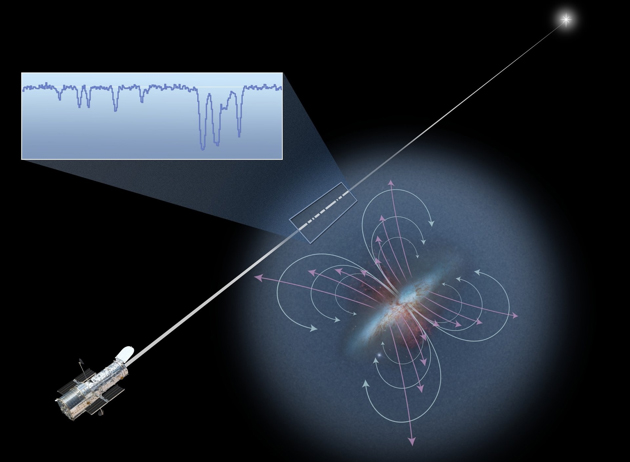
\includegraphics[width=0.95\textwidth]{Introduction/figures/hubble_cgm.jpg}
        \caption{\small{An artist's impression of the CGM of a galaxy. Image credit: NASA/STScI/Ann Field.}}
        \vspace{5pt}
        \label{cgm_artist}
\end{figure}

The current standard model of structure formation is given by Lambda Cold-Dark-Matter ($\Lambda$CDM) cosmology, which predicts the hierarchical growth of large scale structures seeded by initial fluctuations in the dark matter background. In this picture, both galaxies and the IGM should follow the same underlying density profile (e.g., \citealt{fukugita2006, frieman2008} and references therein). Some observational evidence of this large-scale relationship has appeared recently, such as \cite{wakker2015}, who showed that $\rm Ly\alpha$ absorption strength (equivalent width; EW) traces the overall distribution of galaxies in a Cosmic Web filament. Figure \ref{wakker_filament} shows their plot of the EW of $\rm Ly\alpha$ absorbers as a function of distance to the center of a galaxy filament, with the enhanced absorption strength evident close to the filament center. In addition, numerous studies have shown that $\rm Ly\alpha$ absorbers also trace individual galaxy halos (e.g., \citealt{lanzetta1995, chen1998, chen2001a,  tripp1998, bowen2002, cote2005, wakker2009, steidel2010, prochaska2011, thom2012, stocke2013, tumlinson2013, liang2014, danforth2016}). 


\begin{figure}[ht!]
        \centering
        \vspace{0pt}
        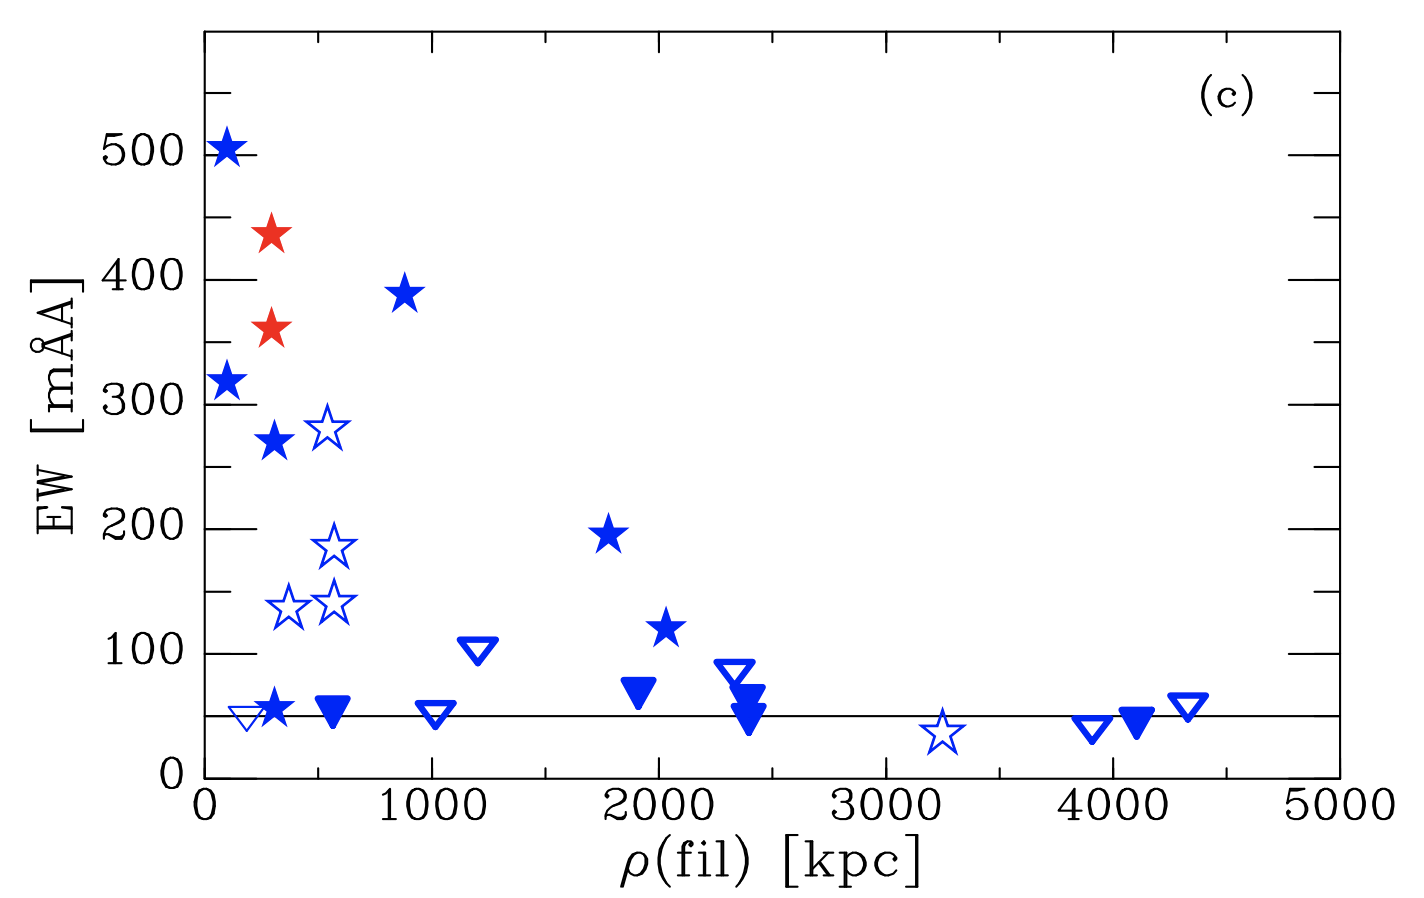
\includegraphics[width=0.8\textwidth]{Introduction/figures/Wakker2015_filament_EW.png}
        \caption{\small{The EW of $\rm Ly\alpha$ absorbers as a function of distance to the center of a galaxy filament. Blue downward tracing triangles indicate upper limits for non-detection, and all stars indicate detections with red stars for detections within a galaxy's virial radius and blue for those far from any known galaxy. See \cite{wakker2015}.}}
        \vspace{5pt}
        \label{wakker_filament}
\end{figure}

\begin{figure}[ht!]
        \centering
        \vspace{0pt}
        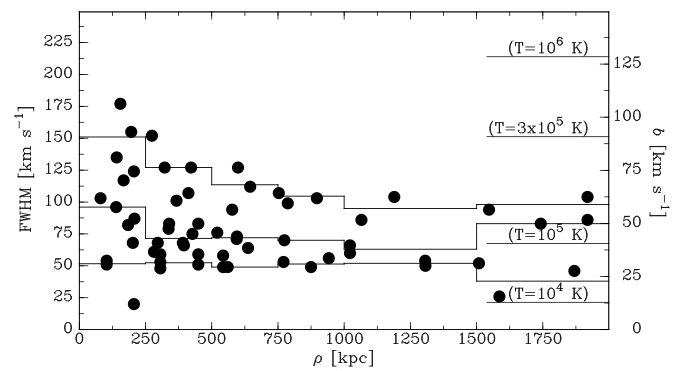
\includegraphics[width=0.8\textwidth]{Introduction/figures/bart_moneyplot.png}
        \caption{\small{The linewidth (or Doppler $b$-parameter) and FWHM of $\rm Ly\alpha$ absorbers as a function of physical impact parameter to the nearest galaxy. Histograms show the 10th, 50th, and 90th percentiles of the distribution.  See \cite{wakker2009}.}}
        \vspace{5pt}
        \label{wakker2009_linewidth}
\end{figure}

The majority of these studies have reported tentative evidence for enhanced $\rm Ly\alpha$ absorption strength with increasing galaxy proximity. The studies of \cite{cote2005} and \cite{prochaska2006} found that about half of $\rm Ly\alpha$ absorbers lie within galaxy halos, at impact parameters $\rho \lesssim 350$ kpc. In addition, \cite{wakker2009} found that for 90\% of $L > 0.1 L^{\**}$ galaxies an absorber can be found within 400 kpc and 400 \kms~, and all galaxies have a $\rm Ly\alpha$ absorber within 1.5 Mpc. Higher redshift studies, such as \cite{rudie2012a} at $2 < z < 3$, find evidence for an elevated density of absorbers up to 2 Mpc from galaxies. \cite{wakker2009} also confirmed a previously suggested correlation between $\rm Ly\alpha$ absorption linewidth (also called Doppler $b$-parameter) and impact parameter ($\rho$), observing that the broadest lines (FWHM $>150$ \kms) are only seen within 350 kpc of a galaxy, while only narrower lines (FWHM $<75$ \kms) are found at $\rho > 1$ Mpc (see Figure \ref{wakker2009_linewidth}). The more recent COS-Halos survey (\citealt{tumlinson2013} and references therein) studied both the \HI~and low-to-medium ionization state metals CGM around $\sim L^{\**}$ galaxies, and found that \HI~is detected nearly ubiquitously within $\sim150$ kpc of both star-forming and passive galaxies, with metal absorption lines also detected in the majority of cases but with a stronger dependence on galaxy type (e.g., \citealt{tumlinson2011b, werk2013}). 


In addition, studying the enrichment of galaxy halos is necessary for constraining outflow models and informing stellar feedback prescriptions. Directly measuring the velocity field and column densities of absorbers as a function of impact parameter and orientation around galaxies would provide the clearest evidence of inflow or outflow activity, but results are few and uncertain. \cite{kacprzak2011_inclination} claim to find that Mg\II~ equivalent widths correlate with galaxy inclination but \cite{mathes2014} find no such correlation for $\rm Ly\alpha$ and O\VI~absorbers. Furthermore, we should expect outflowing gas to be more highly enriched and trace the metallicity of the associated galaxy, with inflowing gas instead appearing only in \HI. Both \cite{stocke2013} and \cite{liang2014} find an ``edge" to heavy ion absorption at $\sim 0.5 R_{\rm vir}$, but with $\rm Ly\alpha$ covering fractions of $\sim 0.75 - 1$ continuing out to $R_{\rm vir}$. However, \cite{mathes2014} measure O\VI~absorption out to $\sim 3 R_{\rm vir}$.


All these previous studies have suffered from small sample sizes (most with fewer than 50 systems), and incompleteness due to their higher mean redshifts where it is increasingly difficult to detect faint galaxies surrounding absorption systems. This thesis aims to address some of these issues by compiling the largest-yet survey of $\rm Ly\alpha$ absorbers spread across a range of environments, and both near and far from galaxies. The installation of the Cosmic Origins Spectrograph (COS; \citealt{green2012}) on the \emph{Hubble Space Telescope} ($HST$) has opened up a new era for studying intergalactic gas via UV QSO-absorption lines, as COS is able to observe fainter targets than ever before with high signal to noise and velocity resolution. Over 700 QSOs have now been observed with COS, most of which have good quality data covering the $\rm Ly\alpha$ transition in the nearby Universe ($cz \leq 10,000$ \kms), where the existing galaxy data is also good and relatively complete to $\sim 0.1 L^{\**}$ on average. 

This project aims to take advantage of all this existing data to study the $\rm Ly\alpha$ traced CGM in the local universe with a survey of unprecedented size. In Chapter 1 I describe the compilation of a new nearby galaxy catalog to take advantage of the existing galaxy data. This catalog is then correlated with the over 700 archival QSO targets observed by the Cosmic Origins Spectrograph (COS) on the Hubble Space Telescope (HST) to produce a sample of galaxy-absorption line systems including a range of galaxy environments, orientations, and types. In the following section I summarize the 3 major questions this thesis aims to tackle with the resulting dataset.

%The CGM is commonly split into a two gas phases: a hot, mostly collisionally ionized phase with gas temperatures near $T\gtrsim 10^6$ K, and a cool, mostly photoionzied phase with gas temperatures near $T \lesssim 10^4$ K.

%\cite{lanzetta1995, bowen1996, chen2008, steidel2010, prochaska2011b, wakker2009}



\section{Science Goals}
While there are numerous open questions concerning the interactions of galaxies and the gas that surrounds them, this thesis focuses on the following:

%1. \emph{Do the physical properties of absorbers depend on their location and orientation with respect to galaxies?}
%2.
%3.
%4.

\subsection{Galaxy Proximity}
\emph{How strongly is intergalactic gas concentrated near galaxies, and does the presence of galaxies affect the physical properties of absorbers?} Recent studies find that half of all $\rm Ly\alpha$ absorbers lie within galaxy halos, at impact parameters of $\rho <350$ kpc and within $400$ \kms~of a galaxy (e.g., \citealt{cote2005, prochaska2006, wakker2009}). Furthermore, \cite{sorini2018} find that the ``sphere of influence" of galaxy can extend all the way to $\sim 2$ Mpc, far more distant than the $\sim150$ kpc or $\sim 1 R_{\rm vir}$ often used as the search radius for CGM studies. However, this may just be an effect of galaxies being embedded in filaments, and not necessarily evidence of the influence of the galaxies themselves. The properties of the lines also appear to change with impact parameter. For example, it has been known for some time that higher column density absorption is found closer to galaxies, and there is good evidence that the same is true for absorption linewidth (e.g., \citealt{wakker2009, prochaska2011}). However, it remains unclear which physical process is responsible; increased turbulence, temperature, ionizing radiation field, or an effect of velocity gradients or blending of multiple cloudlets along the line of sight. Studying this phenomenon as a function of environment with good understanding of the properties, morphologies, and group memberships of the nearby galaxies is the clearest way forward on this question, and a larger statistical sample then previously employed will be required.


\subsection{Galaxy Orientation}
\emph{Do the physical properties of absorbers depend on their orientation with respect to nearby galaxies?} Recent results suggest that absorbing systems have a preferred orientation with respect to the major and minor axes of the galaxies they are near to (e.g., \citealt{kacprzak2011_inclination, kacprzak2012}). This could be evidence of inflows and outflows, an effect of the global structure of galaxy halos, or a signature of a preferred orientation of galaxy halos within Cosmic Web filaments. Unfortunately the statistics are not yet good enough to distinguish between these possible scenarios. Additionally, very few authors (see, e.g., \citealt{mathes2014, bordoloi2014}) have investigated the dependence of absorber properties on nearby galaxy \emph{inclination}, the results of which could have important implications for galaxy halo shape and the spatial dependence of halo gas covering fractions. A large-scale study into the inclination and azimuth angle dependence of absorption is the clearest path forward here.

%\cite{mathes2014} and \cite {bordoloi2011} find little evidence for inclination dependence for O\VI and Mg\II absorbers, but the models of \cite{bordoloi2014} predict 

\subsection{Galaxy Rotation}
\emph{Does intergalactic gas ``know" about the rotation of the galaxies embedded within it?} In particular we would like to know how far out (or to what impact parameter) the rotational curves of galaxies extend, or in other words what angular momentum information is retained by galaxy halos. Galaxy disks are built via accretion of material from the IGM, which caries with it angular momentum. This angular momentum must eventually contribute to the disk rotation, so it is reasonable to expect the overall rotation signature of halo gas to trace that of the more readily measured disk gas rotation. Indeed, the simulations of \cite{stewart2011a, stewart2011b, stewart2013} predict that \HI gas out to at least $1 R_{\rm vir}$ should co-rotate with galaxies, and furthermore that absorption lines in QSO sightlines should be able to accurately trace this (see Figure \ref{stewart_rotation}; a simulated galaxy halo showing coherent halo gas rotation from \citealt{stewart2011a}). Previous studies (e.g., \citealt{steidel2002, cote2005, wakker2009, kacprzak2011_kinematics}) were unable to find a clear correlation between the rotation of galaxy disks and the kinematics of nearby absorbers. However, none of these previous studies have been able to produce a sample of more than a handful of systems, and have only considered the possibility of an extended, warped stellar disk in their analysis. A targeted observational campaign for easily observed galaxies in the local Universe could make substantial progress here.


\begin{figure}[t!]
        \centering
        \vspace{0pt}
        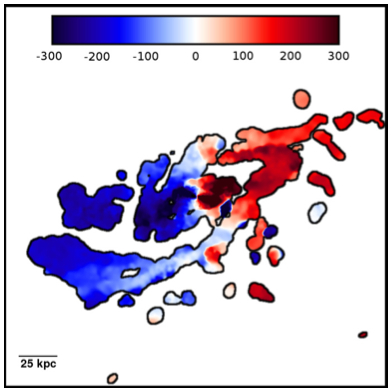
\includegraphics[width=0.7\textwidth]{Introduction/figures/stewart2011_comoving_gas.jpg}
        \caption{\small{A simulated galaxy halo showing the coherent co-rotation of halo gas out at least 100 kpc from the inner disk (the galaxy disk is seen in dark blue and red at the image center; see \cite{stewart2011a}).}}
        \vspace{5pt}
        \label{stewart_rotation}
\end{figure}




\section{Summary of Thesis}
In the following chapters I describe a program to observationally explore the connections between low column density $\rm Ly\alpha$ absorption and the galaxy environment in the local Universe. This program focuses mainly on archival QSO observations taken by the Cosmic Origins Spectrograph (COS) on the Hubble Space Telescope (HST), and correlations between the locations of detected $\rm Ly\alpha$ absorption and of galaxies larger than $\sim 0.1 L^{\**}$. By restricting our study to low-redshifts ($cz \leq 10,000$ \kms) we are able to compile a dataset of unparalleled size while remaining highly complete to galaxies of all types, sizes, and distances from absorption detections. The results of this thesis are presented as follows:

\begin{enumerate}

\item{In Chapter 1 I present a new nearby galaxy catalog. In order to study the CGM-galaxy connection on a large, all-sky scale, we rely heavily on archival, publicly available data for the positions and properties of the galaxies. We describe the retrieval, handling, homogenization and completeness of these data, as well as detailed descriptions of each included galaxy property (i.e., the catalog columns).}

 
\item{In Chapter 2 I present the results of a pilot study with 33 QSO sightlines chosen for their proximity to large galaxies ($D \ge 25$ kpc). We introduce a new method for absorber-galaxy matching called the likelihood-method, which will make it possible to algorithmically study our large final data set. Using this likelihood-method we match 48 $\rm Ly\alpha$ absorption lines with nearby large galaxies, and study the absorption strength (EW) as a function of velocity and spatial separation, azimuth angle and inclination. We find that the strongest absorbers are all found within $100$ \kms~of a galaxy, and that there exists an overabundance of detections near highly inclined galaxies ($inc \gtrsim 50^{\circ}$). We attribute this overabundance to the effect of flattened, non-spherical galaxy halos on the detection probability as a function of impact parameter.}


\item{In Chapter 3 I present the results of a study of the kinematic connection between galaxy disks and $\rm Ly\alpha$-traced halo gas. We have compiled a sample of 29 galaxies with known rotation curves both from the literature and from new observations with the Southern African Large Telescope (SALT) which also appear within $3 R_{\rm vir}$ of a COS QSO sightline. We compare the galaxy disk kinematics to the velocities of $\rm Ly\alpha$ absorption lines detected in 19 nearby QSO sightlines with the help of custom cylindrical and NFW-based halo rotation models \citep{navarro1996, navarro1997}. We find that the co-rotation fraction of absorbers declines as a function of galaxy luminosity, which we attribute to the effect of cold-mode accretion dominating in lower-mass galaxy halos.}


\item{In Chapter 4 I present the results of our full CGM survey, which includes 1135 $\rm Ly\alpha$ absorbers detected in the spectra of 264 QSO spectra. We explore the effect of different normalizations to our likelihood-method for absorber-galaxy matching, and use this technique to split absorber-galaxy systems into 5 different bins based on their galaxy environments. We find that both absorption strength (EW) and linewidth (Doppler $b$-parameter) are enhanced with proximity to a single galaxy, and further enhanced by proximity to multiple galaxies. We also detect a bimodal azimuth distribution, with $\rm Ly\alpha$ absorbers preferentially found slightly offset from both the minor and major galaxy axes. We confirm the inclination results first suggested in Chapter 2.}

\item{ In Chapter 5 I summarize the results of this thesis, and place these results in the broader context of the circumgalactic medium and it's implications for global galaxy evolution.}

\end{enumerate}

%\nocite{*}
%\bibliography{/Users/frenchd/Research/bib}{}
\bibliographystyle{thesis}
\bibliography{/Users/clairemurray/Desktop/DMF_thesis/bib}{}



\chapter[A Catalogue of Nearby ($cz \leq 10,000$ \kms) Galaxies]{A Catalogue of Nearby ($cz \leq 10,000$ \kms) Galaxies} 
\label{chap:chap2}

% Leave space between title and quote or publication note.  This has often been
% 10cm for a quote and 8 cm for a reference, but this is really up to you.
%\vspace{8cm}

\vfill

\begin{flushright}
  \fixspacing % Single spacing
  \textit{To be submitted to the \emph{Astrophysical Journal}} \\
%  \vspace{1ex} Tofflemire, et al.\ 2017, \apj, 835, 8
\end{flushright}

\vspace*{1in} % Leave a 1-in space at the bottom.

\cleardoublepage

%\nocite{*}

%%\documentclass[iop]{emulateapj-rtx4}
%
%\documentclass[twocolumn,tighten]{aastex62}
%
% \shortauthors{French $\&$ Wakker}
%\usepackage{graphicx}
%\usepackage{subfigure}
%\usepackage{amsmath}
%
%
%%\usepackage{graphicx}
%%\usepackage{amssymb}
%%\usepackage{wrapfig}
%%\usepackage{setspace}
%%\usepackage{subfigure}
%%\usepackage{mathtools}
%%\usepackage{hyperref}
%
%
%\newcommand{\kms}{$\rm km\, s^{-1}$}
%
%\graphicspath{{figures//}}
%
%\frenchspacing
%
%\begin{document}
%
%
%\title{A Catalogue of Nearby ($cz \leq 10,000$ \kms) Galaxies}
%
%\author{David M. French, Bart P. Wakker}
%
%\affil{Department of Astronomy, University of Wisconsin - Madison}


\begin{chabstract}
We present an all-sky catalogue of galaxies with recession velocity $cz \leq 10,000$ \kms. We used published data available through the NASA Extragalactic Database (NED), the NASA/IPAC Infrared Science Archive (IRSA), the Third Reference Catalogue of Bright Galaxies (RC3), and the \cite{tully2015} 2MASS galaxy group catalogue. We homogenized the combined dataset by converting diameter measurements to 2MASS values, and employing outlier rejection to choose representative values for position angle, inclination, redshift-independent distance, and $B$-band magnitude. We use these values to estimate galaxy $B$-band luminosities.

%\citep[][]{tully2015}
%\cite[][]{tully2015}

\end{chabstract}

\cleardoublepage

%\keywords{IGM, CGM, galaxies}


\section{Introduction}

Galaxy catalogues form the basis for all studies of the nearby universe, as they are needed to create representative samples, study the distribution of galaxies, among many other things. The ideal solution of an all-sky and all-object online database containing homogenized information has not been completely realized, even as the NASA Extragalactic Database (NED)\footnote{https://ned.ipac.caltech.edu/}, Vizier\footnote{http://vizier.u-strasbg.fr/}, SIMBAD\footnote{http://simbad.u-strasbg.fr/simbad/} and others approach some of these requirements. Each of these databases offer slightly different sets of information on their objects, and there is often no straightforward way for extracting all the parameters needed. Moreover, these aggregation sites typically contain all published parameters with no judgment of their quality. For example, there is no way to return the diameters of all known galaxies in a particular redshift range. Furthermore, comparing and choosing between disparate measurements of common galaxy parameters (e.g., diameter, inclination, magnitude, distance, etc.) is not trivial when a large sample is required. The need for a simple, highly complete easy-lookup nearby galaxy catalogue remains.

For our studies of the circumgalactic medium (CGM) around galaxies in the nearby universe we required just such a galaxy dataset, with a high degree of completeness and homogeneity. Therefore we have constructed a catalogue of galaxies within the redshift range $cz \leq 10,000$ \kms. All of the data included here is publicly available through the NASA Extragalactic Database (NED), the NASA/IPAC Infrared Science Archive (IRSA), the Third Reference Catalogue of Bright Galaxies (RC3; \citealt{RC3}), and the \cite{tully2015} 2MASS Galaxy Group Catalog. We have endeavored in various ways to create a single, homogeneous catalogue. The largest effort on this front revolved around deriving consistent linear and angular galaxy diameters. While we originally began compiling this data base as a tool to aid in the matching of galaxies to absorption detected in background QSO spectra,  we hope that it can prove useful to the community at large. 

In Section 2 we discuss our data retrieval methods and handling of distance and velocity measurements. In Section 3, we provide explanation and details for each galaxy attribute included in the catalogue (i.e., the data columns). We discuss caveats and limitations in Section 4. Throughout this catalogue we have adopted the cosmology $H_{\rm 0}$ = 71 \kms ~$\rm Mpc^{-1}$, $\rm \Omega_m$ = 0.27, and $\rm \Omega_{\Lambda}$=0.73 when converting recession velocities into distances.

\section{Data}

\subsection{Data Retrieval}

All data contained in this catalogue \emph{except} for extinction, RC3 parameters, and group membership were retrieved from NED. Our criterion for including a galaxy in this dataset is only a published redshift which places the galaxy in the $cz \leq 10,000$ \kms~velocity range.  These data were retrieved from NED in a two-step process. First, we used the NED ``Search By Parameters" service to retrieve all objects with classification type ``Galaxies (G)" and heliocentric velocity $\leq 10,000$ \kms. Because of a 10,000 object retrieval cap imposed by NED, this step was completed in 14 separate redshift steps. Next, we used the retrieved list of object names to query NED for more detailed information than is available through the initial search. We completed this query using a suite of custom Python scripts which retrieve the object's XML VOTable, which contains \emph{all} object information and measurements contained in NED. 

We then retrieved the Galactic dust extinction ($E(B-V)$) estimates produced by \cite{schlafly2011} toward each object from the Galactic Dust Reddening and Extinction service hosted by the NASA/IPAC Infrared Science Archive (IRSA) \footnote{http://irsa.ipac.caltech.edu/applications/DUST/}. Again, this took several steps because of the 20,000 row limit imposed by the Table Upload mode offered by IRSA. Group information (membership; \S \ref{group_num}, number of members; \S \ref{group_mem}, and group distance; \S \ref{group_dist}) for each galaxy was taken from the 2MASS Galaxy Group Catalogue \cite{tully2015}. Finally, we also include the galaxy type (\S \ref{RC3_type}), position angle (\S \ref{RC3_pa}), apparent major isophotal diameter (\S \ref{RC3_d25}), and major-to-minor axis ratio (\S \ref{RC3_r25}) from the Third Reference Catalogue of Bright Galaxies (RC3; \S \citealt{RC3}) for the 18,601 galaxies in this catalogue.

\subsection{Completeness} \label{completeness}

\begin{figure}[ht!]
        \centering
        \vspace{0pt}
        \includegraphics[width=0.8\textwidth]{Chap2/figures/Lstar_histogram_4bins_final_0-10000_v3_vert_flag0.pdf}
        \caption{\small{Distribution of $L/$\Lstar values  for all galaxies in the dataset. Black vertical lines highlight 1, 0.5, 0.1, 0.05 and 0.01 \Lstar. The turnoff in the distribution for each region reveals the corresponding completeness. We are highly complete to 0.01\Lstar out to 2500 \kms~, 0.05\Lstar between $2500 \leq cz \leq 5000$ \kms, 0.1\Lstar between $6000 \leq cz \leq 8000$ \kms, and 0.3\Lstar $8000 \leq cz \leq 10000$ \kms. See \S \ref{completeness} for a discussion of these limits.}}
        \vspace{5pt}
        \label{completeness_plot}
\end{figure} 

\begin{figure}[ht!]
        \centering
        \vspace{0pt}
        \includegraphics[width=0.99\textwidth]{Chap2/figures/hist_by_survey8_filtered_0only.pdf}
        \caption{\small{Number of objects included from the major sources 2MASS (solid-black), SDSS (dashed-red), 2dF (solid-gold-crosses), 6dF (dot-dashed-green), RC3 (dotted-diamond-blue) and all other sources (solid-grey) plotted as a function of heliocentric velocity. The peak for ``other sources" between $2500 \lesssim v_{\rm hel} \lesssim 3100$ \kms~is due to the small (1.3 square degrees) ultra-deep Suburu/XMM-Newton Deep Sky Survey (SXDS), which reaches a $B$-band magnitude limit of $B=28.2$.}}
        \vspace{5pt}
        \label{source_histograms}
\end{figure} 


%\begin{figure}[htb]
%        \centering
%        \vspace{0pt}
%        \includegraphics[width=0.999\textwidth, angle=90]{Chap2/figures/all_sky.pdf} \label{a}
%        \includegraphics[width=0.99\textwidth, angle=90]{Chap2/figures/all_sky_6h.pdf} \label{b}
%        \includegraphics[width=0.99\textwidth, angle=90]{Chap2/figures/all_sky_12h.pdf} \label{c}
%        \caption{\small{The positions of all galaxies with $flag=0$ (see \ref{flag} below) plotted in Aitoff projection and colored according to heliocentric velocity. We include 3 maps, centered at \textbf{Top:} R.A. = 0h, \textbf{Center:} R.A. = 6h, and \textbf{Bottom:} R.A. = 12h. }}
%%        \vspace{5pt}
%        \label{allskyvhel}
%\end{figure}


\begin{figure}[htb!]
        \centering
        \vspace{0pt}
        \includegraphics[width=0.55\textwidth, angle=0]{Chap2/figures/all_sky.pdf} \label{a}
        \caption{\small{The positions of all galaxies with $flag=0$ (see \ref{flag} below) plotted in Aitoff projection and colored according to heliocentric velocity. We include 3 maps, centered here at R.A. = 0h. See below for R.A. = 6h and R.A. = 12h centered maps.}}
%        \vspace{5pt}
        \label{allskyvhel}
\end{figure}
\begin{figure}[htb!]\ContinuedFloat
        \centering
        \vspace{0pt}      
        \includegraphics[width=0.55\textwidth, angle=0]{Chap2/figures/all_sky_6h.pdf} \label{b}
        \caption{\small{The positions of all galaxies with $flag=0$ (see \ref{flag} below) plotted in Aitoff projection and colored according to heliocentric velocity. We include 3 maps, centered here at R.A. = 6h. See above and below for R.A. = 0h and R.A. = 12h centered maps.}}
%        \vspace{5pt}
        \label{allskyvhel}
\end{figure}
\begin{figure}[htb!]\ContinuedFloat
        \centering
        \vspace{0pt}
        \includegraphics[width=0.55\textwidth, angle=0]{Chap2/figures/all_sky_12h.pdf} \label{c}
        \caption{\small{The positions of all galaxies with $flag=0$ (see \ref{flag} below) plotted in Aitoff projection and colored according to heliocentric velocity. We include 3 maps, centered here at R.A. = 12h. See above for R.A. = 0h and R.A. = 6h centered maps.}}
%        \vspace{5pt}
        \label{allskyvhel}
\end{figure}



The galaxy dataset contains 130,819  objects, and includes data from SDSS, 2MASS, 2dF, 6dF, RC3, and many other, smaller surveys. Figure \ref{completeness_plot} shows the number of objects as a function of luminosity in four bins of heliocentric velocity, and Figure \ref{source_histograms} shows the number of objects coming from each of the major included surveys as a function of heliocentric velocity.\footnote{The peak for ``other sources" between $2500 \lesssim v_{\rm hel} \lesssim 3100$ \kms~in Figure \ref{source_histograms} is due to the small (1.3 square degrees) ultra-deep Suburu/XMM-Newton Deep Sky Survey (SXDS), which reaches a $B$-band magnitude limit of $B=28.2$. See https://www.naoj.org/Science/SubaruProject/SXDS/} Our restricted velocity range of $cz \leq 10,000$ \kms~leads to a completeness limit of $B \lesssim 18.7$ mag, or $\sim0.2$\Lstar, at $cz = 10,000$ \kms, and progressively better towards lower velocities (see Figure \ref{completeness_plot}). This limit will vary depending on which major surveys include a particular region of the sky. The major contributor is whether or not SDSS data is available, which begins around $cz = 5,000$ \kms. Figure \ref{completeness_plot} is split into 4 velocity bins to illustrate this. Our data has a high degree of completeness down to $\sim0.01$\Lstar in the first bin, $0 \leq cz \leq 2,500$ \kms. At slightly higher velocity, $2500 \leq cz \leq 6000$ \kms, the completeness falls a bit, but is still rather complete to $\sim0.05$\Lstar as we move past the near and well studied galaxies, but have yet to reach the footprint of deep all sky surveys. SDSS data becomes available in the last two bins, spanning $6000 \leq cz \leq 10,000$ \kms, and correspondingly completeness remains high down to the SDSS limits of $B \lesssim 18.7$ mag, or $\sim0.2$\Lstar at $cz = 10,000$ \kms. 


Additionally, we note the presence of a long super-faint tail to the distribution in the low velocity bin ($0 \leq cz \leq 2,500$ \kms. This is due to a number of pointed, ultra-deep surveys which have picked up faint dwarfs in the very local universe, which then quickly exit the observability window past $v_{\rm hel} \sim 2500$ \kms. All luminosities are calculated as described below in \S \ref{Lstar_med}.




\section{The Catalogue}
The following section describes the contents of each column in the order it appears in the catalogue. Null values are marked in one of three ways. Columns containing strings have the null value of 'x', those containing integers have null value '-99', and those containing floating point entries have null value '-99.99'. The following subsection numbers correspond to the column numbers in the catalogue (i.e., \S \ref{Name} is the first data column, \S \ref{NEDname} is the second, etc.).

\subsection{Name} \label{Name}
Our preferred name for the galaxy. If the galaxy is in one of the following base catalogues we adopt that name, in the order of preference given below. If the galaxy is not in one of these catalogues, we use the NED-preferred name (\S \ref{NEDname}).

Name preferences: NGC, IC, UGC, UGCA, Mrk, SBS, Fairall, TOLOLO, Ton, ESO, Holm, MCG, CGCG, IRAS, IRASF, KISS, KISSR, Kaz, IZw, IIZw, IIIZw, IVZw, VZw, VIZw, VIIZw, SDSS, 3C, PG, HE, HS, PKS, FCC, FGC, HCG, VCC, KUG, PGC, 2MASS, 2dF, 6dF.

%Name preferences: NGC, IC, Mrk, UGC, UGCA, PHL, 3C, SBS, MCG, ESO, TON, TONS, PGC, PG, PB, FGC, HS, HE, KUG, IRAS, RX, CGCG, KAZ, FCC, FAIRALL, HOLM, IZw, IIZw, IIIZw, IVZw, VZw, VIZw, VIIZw, VIIIZw, IRAS, IRASF, KISS, KISSR, FBQS, LBQS, PKS, SDSS, VCC, 2MASS, 2DF, 6DF, HIPASS, 2MASX.

%NGC, MRK, UGC, PHL, 3C, IC, SBS, MCG, ISO, TON, PGC, PG, PB, FGC, HS, HE, KUG, IRAS, RX, CGCG, FBQS, LBQS, SDSS, VCC, 2MASS, 2DF, 6DF, HIPASS, 2MASX, MESSIER. 

\subsection{NEDname} \label{NEDname}
The preferred name for the galaxy in the NED database.

\subsection{z} \label{z}
The NED-preferred redshift for the galaxy. 

\subsection{RAdeg} \label{RAdeg}
Equatorial right ascension coordinate in degrees (J2000.0 epoch).

\subsection{DEdeg} \label{DEdeg}
Equatorial declination coordinate in degrees (J2000.0 epoch).

\subsection{RAh} \label{RAh}
Equatorial right ascension hour coordinate (J2000.0 epoch).

\subsection{RAm} \label{RAm}
Equatorial right ascension minute coordinate (J2000.0 epoch).

\subsection{RAs} \label{RAs}
Equatorial right ascension second coordinate (J2000.0 epoch).

\subsection{DE-} \label{DE-}
Equatorial declination coordinate sign (J2000.0 epoch).

\subsection{DEd} \label{DEd}
Equatorial declination degree coordinate (J2000.0 epoch).

\subsection{DEm} \label{DEm}
Equatorial declination minute coordinate (J2000.0 epoch).

\subsection{DEs} \label{DEs}
Equatorial declination second coordinate (J2000.0 epoch).

\subsection{GLON} \label{GLON}
Galactic longitude coordinate.

\subsection{GLAT} \label{GLAT}
Galactic latitude coordinate.

\subsection{Vhel} \label{Vhel}
Heliocentric radial velocity in \kms~units. As done by NED, we do not make any relativistic correction to these velocities.

\subsection{vcorr} \label{vcorr}
Virgocentric flow-corrected velocity. Following \cite{huchra1982, geller1983}, this is calculated as
\begin{gather*}
	vcorr = v_{\rm hel} + 300*[\sin(decl) \sin(12^{\circ}.9333) \\
	+ \\
	\cos(decl) \cos(12^{\circ}.9333) \cos(R.A. - 186^{\circ}.7833),
\end{gather*}

\noindent which corresponds to a velocity of 300 \kms~ toward $R.A. = 186^{\circ}.7833$, $decl. = 12^{\circ}.9333$.

%\begin{eqnarray}
%\begin{centering}
%	\nonumber
%	vcorr = v_{\rm hel} + 300*[\sin(decl) \sin(12^{\circ}.9333) \\
%	\nonumber
%	+ \\
%	\cos(decl) \cos(12^{\circ}.9333) \cos(R.A. - 186^{\circ}.7833)]
%\end{centering}
%\end{eqnarray}


\subsection{distvcorr} \label{distvcorr}
Distance calculated from $vcorr$ with a Hubble constant of $H_0 = 71$ \kms $~\rm Mpc^{-1}$.

\subsection{RID\_mean} \label{RID_mean}
Mean redshift-independent distance from the NED-D catalogue \citep{tully2009}. This is the arithmetic mean of the available measurements and therefore does not correspond to any single measurement in particular.

\subsection{RID\_median} \label{RID_median}
Median redshift-independent distance from the NED-D catalogue. This is not the arithmetic median of the set, but rather the published distance value \emph{closest} to the median. The method used for this distance estimate is given by \emph{distIndicator} (\S \ref{distIndicator}).

\subsection{RID\_std} \label{RID_std}
Standard deviation of all redshift-independent distance measurements.

\subsection{RID\_min} \label{RID_min}
Minimum published redshift-independent distance.

\subsection{RID\_max} \label{RID_max}
Maximum published redshift-independent distance.

\subsection{bestDist} \label{bestDist}
Our chosen best distance estimate. This is equal to $RID\_median$ when a redshift-independent distance is available, and otherwise defaults to $distvcorr$. A redshift-independent distance estimate is available for 17,361 objects, which corresponds to 13.3\% of all objects in the catalogue. For these objects $bestDist$ is set to the median of all available redshift-independent distance estimates, and $e\_bestDist$ (\S \ref{e_bestDist}) is set to the published observational error for this median value. If no error is available, $e\_bestDist$ is instead set to the standard deviation of all available redshift-independent distance measurements. When only a redshift is available, we set $bestDist$ equal to $distvcorr$ (\S \ref{distvcorr}), which is the the Hubble law distance as calculated with $H_{\rm 0} = 71$ \kms~$\rm Mpc^{-1}$ and a Virgocentric flow-corrected velocity ($vcorr$; \S \ref{vcorr}). The associated error, $e\_bestDist$, is then set to 10\% of the resulting distance estimate. At very low redshift, the uncertainty in this estimate is dominated by deviations from the Hubble Flow due to, e.g., the Local Group, and at larger distances the uncertainty in $H_{\rm 0}$ becomes dominant. The distance error for any particular galaxy is difficult to ascertain, but a 10\% error should contain the true $1\sigma$ error across our full redshift range. All galaxies with zero or negative $Vhel$ have $bestDist$ set to 1 Mpc, and $e\_bestDist$ to 0.5 Mpc (unless a redshift-independent distance is available). 

\subsection{e\_bestDist} \label{e_bestDist}
The error on $bestDist$. $e\_bestDist$ is equal to $RID\_std$ when a redshift-independent distance is available. Otherwise, $e\_bestDist$ is set to 10\% of $distvcorr$ when $vcorr \geq 0$, and 50\% of $distvcorr$ if $vcorr < 0$.


\subsection{distIndicator} \label{distIndicator}
A key indicating which method was used to measure the redshift-independent distance for this galaxy. Table \ref{distIndicators} shows the keys and their corresponding full names as compiled in the NED-D distance catalogue. This key corresponds \textit{only} to the $RID\_median$ value.


%\startlongtable
\begin{deluxetable}{llll}
\tablewidth{0pt}
\tabletypesize{\footnotesize}
\tablecaption{Distance Indicator Keys\label{distIndicators}}
\tablehead{
\colhead{Key}  	&  \colhead{Distance Indicator} 	&  \colhead{Key}	&  \colhead{Distance Indicator} }
\startdata
    AGB	&	AGB					&	MagEn    	&	Magnetic energy    	\\
    AGNtl	&	AGN time lag    		&	Mag    	&	Magnitude    	\\
    Bstar	&	B Stars				&	Maser    	&	Maser    	\\
    BCG	&	BCG					&	MassM    	&	Mass Model    	\\
    BH	&	Black Hole			&	Miras   	&	Miras    	\\
    BLLum	&	BL Lac Luminosity		&	Novae    	&	Novae    	\\
    BSG    	&	Blue Supergiant		&	OBstr    	&	OB Stars    	\\
    Brstr    	&	Brightest Stars    		&	OrMec    	&	Orbital Mech.    	\\
    Cstar    	&	Carbon Stars    			&	PAGB    	&	PAGB Stars    	\\
    Ceph    	&	Cepheids				&	PNLF    	&	PNLF    	\\
    CMD    	&	CMD					&	propM    	&	Proper Motion    	\\
    dCO    	&	CO ring diameter		&	QS    	&	Quasar spectrum    	\\
    Dsigm	&	D-Sigma				&	Radio    	&	Radio Brightness    	\\
    Scuti	&	Delta Scuti    			&	RClum    	&	Red Clump    	\\
    Diam	&	Diameter				&	DRing    	&	Ring Diameter    	\\
    dwEll	&	Dwarf Ellipticals    		&	RRLyr    	&	RR Lyrae    	\\
    Dwarf	&	Dwarf Galaxy Diameter	&	RSV    	&	RSV Stars    	\\
    EclBi	&	Eclipsing Binary		&	RV    	&	RV Stars    	\\
    FJ		&	Faber-Jackson			&	SDorS    	&	S Doradus Stars    	\\
    FGLR	&	FGLR				&	SBF    	&	SBF    	\\
    GLens	&	G Lens				&	SGRB    	&	SGRB    	\\
    GCFP	&	GC FP				&	SNIa    	&	SNIa    	\\
    GCKJK	&	GC K vs. (J-K)			&	SNIIo    	&	SNII optical    	\\
    GCrad	&	GC radius				&	SNIIr    	&	SNII radio    	\\
    GCLF	&	GCLF				&	SNIas    	&	SNIa SDSS    	\\
    GCSBF	&	GC SBF				&	Stat    	&	Statistical    	\\
    gamma	&	GeV TeV ratio			&	Sosie    	&	Sosies    	\\
    GSGD	&	Grav. Stability Gas. Disk 	&	subDw    	&	Subdwarf fitting    	\\
    GRB	&	GRB					&	SXPS	&	SX Phe Stars    	\\
    HIod	&	H I + optical distribution	&	SZ    	&	SZ effect    	\\
    HIILF	&	HII LF				&	Terti		&	Tertiary    	\\
    dHII	&	HII region diameter		&	TRGB    	&	TRGB    	\\
    HB	&	Horizontal Branch    		&	TFest    	&	Tully est    	\\
    IRAS	&	IRAS    				&	TF		&	Tully-Fisher    	\\
    Jet	&	Jet Proper Motion    		&	CepII    	&	Type II Cepheids    	\\
    LHbs	&	L(H $\beta$)-$\sigma$	&	WD    	&	White Dwarfs    	\\
    LSB	&	LSB galaxies			&	WR    	&	Wolf-Rayet    	\\
    Mstar	&	M Stars				&			&				\\
\enddata 
\tablecomments{Distance indicators and associated keys. Full descriptions can be found at \url{https://ned.ipac.caltech.edu/Library/Distances/distintro.html}}
\vspace{-5pt}
\end{deluxetable}


%\begin{center}
%\begin{longtable}{llll}
%  \caption[Short caption]{Long captions for the long table.} \label{tab:long1} \\
%  % First head
%  \hline
%  % The table
%    AGB	&	AGB					&	MagEn    	&	Magnetic energy    	\\
%    AGNtl	&	AGN time lag    		&	Mag    	&	Magnitude    	\\
%    Bstar	&	B Stars				&	Maser    	&	Maser    	\\
%    BCG	&	BCG					&	MassM    	&	Mass Model    	\\
%    BH	&	Black Hole			&	Miras   	&	Miras    	\\
%    BLLum	&	BL Lac Luminosity		&	Novae    	&	Novae    	\\
%    BSG    	&	Blue Supergiant		&	OBstr    	&	OB Stars    	\\
%    Brstr    	&	Brightest Stars    		&	OrMec    	&	Orbital Mech.    	\\
%    Cstar    	&	Carbon Stars    			&	PAGB    	&	PAGB Stars    	\\
%    Ceph    	&	Cepheids				&	PNLF    	&	PNLF    	\\
%    CMD    	&	CMD					&	propM    	&	Proper Motion    	\\
%    dCO    	&	CO ring diameter		&	QS    	&	Quasar spectrum    	\\
%    Dsigm	&	D-Sigma				&	Radio    	&	Radio Brightness    	\\
%    Scuti	&	Delta Scuti    			&	RClum    	&	Red Clump    	\\
%    Diam	&	Diameter				&	DRing    	&	Ring Diameter    	\\
%    dwEll	&	Dwarf Ellipticals    		&	RRLyr    	&	RR Lyrae    	\\
%    Dwarf	&	Dwarf Galaxy Diameter	&	RSV    	&	RSV Stars    	\\
%    EclBi	&	Eclipsing Binary		&	RV    	&	RV Stars    	\\
%    FJ		&	Faber-Jackson			&	SDorS    	&	S Doradus Stars    	\\
%    FGLR	&	FGLR				&	SBF    	&	SBF    	\\
%    GLens	&	G Lens				&	SGRB    	&	SGRB    	\\
%    GCFP	&	GC FP				&	SNIa    	&	SNIa    	\\
%    GCKJK	&	GC K vs. (J-K)			&	SNIIo    	&	SNII optical    	\\
%    GCrad	&	GC radius				&	SNIIr    	&	SNII radio    	\\
%    GCLF	&	GCLF				&	SNIas    	&	SNIa SDSS    	\\
%    GCSBF	&	GC SBF				&	Stat    	&	Statistical    	\\
%    gamma	&	GeV TeV ratio			&	Sosie    	&	Sosies    	\\
%    GSGD	&	Grav. Stability Gas. Disk 	&	subDw    	&	Subdwarf fitting    	\\
%    GRB	&	GRB					&	SXPS	&	SX Phe Stars    	\\
%    HIod	&	H I + optical distribution	&	SZ    	&	SZ effect    	\\
%    HIILF	&	HII LF				&	Terti		&	Tertiary    	\\
%    dHII	&	HII region diameter		&	TRGB    	&	TRGB    	\\
%    HB	&	Horizontal Branch    		&	TFest    	&	Tully est    	\\
%    IRAS	&	IRAS    				&	TF		&	Tully-Fisher    	\\
%    Jet	&	Jet Proper Motion    		&	CepII    	&	Type II Cepheids    	\\
%    LHbs	&	L(H $\beta$)-$\sigma$	&	WD    	&	White Dwarfs    	\\
%    LSB	&	LSB galaxies			&	WR    	&	Wolf-Rayet    	\\
%    Mstar	&	M Stars				&			&				\\
%\end{longtable}
%\end{center}




%\begin{center}
%\begin{longtable}{llll}
%%Here is the caption, the stuff in [] is the table of contents entry,
%%the stuff in {} is the title that will appear on the first page of the
%%table.
%\caption[Distance Indicator Keys]{Distance Indicator Keys} \label{distIndicators} \\
%
%%This is the header for the first page of the table...
%\hline \hline \\[-2ex]
%   \multicolumn{1}{c}{Key} &
%   \multicolumn{1}{c}{Distance Indicator} &
%   \multicolumn{1}{c}{Key} &
%   \multicolumn{1}{c}{Distance Indicator} \\[0.5ex] \hline
%   \\[-1.8ex]
%\endfirsthead
%
%%This is the header for the remaining page(s) of the table...
%\multicolumn{4}{c}{{\tablename} \thetable{} -- Continued} \\[0.5ex]
%  \hline \hline \\[-2ex]
%   \multicolumn{1}{c}{Key} &
%   \multicolumn{1}{c}{Distance Indicator} &
%   \multicolumn{1}{c}{Key} &
%   \multicolumn{1}{c}{Distance Indicator} \\[0.5ex] \hline
%  \\[-1.8ex]
%\endhead
%
%%This is the footer for all pages except the last page of the table...
%  \multicolumn{4}{l}{{Continued on Next Page\ldots}} \\
%\endfoot
%
%%This is the footer for the last page of the table...
%  \\[-1.8ex] \hline \hline
%\endlastfoot
%
%%Now the data...
%    AGB	&	AGB					&	MagEn    	&	Magnetic energy    	\\
%    AGNtl	&	AGN time lag    		&	Mag    	&	Magnitude    	\\
%    Bstar	&	B Stars				&	Maser    	&	Maser    	\\
%    BCG	&	BCG					&	MassM    	&	Mass Model    	\\
%    BH	&	Black Hole			&	Miras   	&	Miras    	\\
%    BLLum	&	BL Lac Luminosity		&	Novae    	&	Novae    	\\
%    BSG    	&	Blue Supergiant		&	OBstr    	&	OB Stars    	\\
%    Brstr    	&	Brightest Stars    		&	OrMec    	&	Orbital Mech.    	\\
%    Cstar    	&	Carbon Stars    			&	PAGB    	&	PAGB Stars    	\\
%    Ceph    	&	Cepheids				&	PNLF    	&	PNLF    	\\
%    CMD    	&	CMD					&	propM    	&	Proper Motion    	\\
%    dCO    	&	CO ring diameter		&	QS    	&	Quasar spectrum    	\\
%    Dsigm	&	D-Sigma				&	Radio    	&	Radio Brightness    	\\
%    Scuti	&	Delta Scuti    			&	RClum    	&	Red Clump    	\\
%    Diam	&	Diameter				&	DRing    	&	Ring Diameter    	\\
%    dwEll	&	Dwarf Ellipticals    		&	RRLyr    	&	RR Lyrae    	\\
%    Dwarf	&	Dwarf Galaxy Diameter	&	RSV    	&	RSV Stars    	\\
%    EclBi	&	Eclipsing Binary		&	RV    	&	RV Stars    	\\
%    FJ		&	Faber-Jackson			&	SDorS    	&	S Doradus Stars    	\\
%    FGLR	&	FGLR				&	SBF    	&	SBF    	\\
%    GLens	&	G Lens				&	SGRB    	&	SGRB    	\\
%    GCFP	&	GC FP				&	SNIa    	&	SNIa    	\\
%    GCKJK	&	GC K vs. (J-K)			&	SNIIo    	&	SNII optical    	\\
%    GCrad	&	GC radius				&	SNIIr    	&	SNII radio    	\\
%    GCLF	&	GCLF				&	SNIas    	&	SNIa SDSS    	\\
%    GCSBF	&	GC SBF				&	Stat    	&	Statistical    	\\
%    gamma	&	GeV TeV ratio			&	Sosie    	&	Sosies    	\\
%    GSGD	&	Grav. Stability Gas. Disk 	&	subDw    	&	Subdwarf fitting    	\\
%    GRB	&	GRB					&	SXPS	&	SX Phe Stars    	\\
%    HIod	&	H I + optical distribution	&	SZ    	&	SZ effect    	\\
%    HIILF	&	HII LF				&	Terti		&	Tertiary    	\\
%    dHII	&	HII region diameter		&	TRGB    	&	TRGB    	\\
%    HB	&	Horizontal Branch    		&	TFest    	&	Tully est    	\\
%    IRAS	&	IRAS    				&	TF		&	Tully-Fisher    	\\
%    Jet	&	Jet Proper Motion    		&	CepII    	&	Type II Cepheids    	\\
%    LHbs	&	L(H $\beta$)-$\sigma$	&	WD    	&	White Dwarfs    	\\
%    LSB	&	LSB galaxies			&	WR    	&	Wolf-Rayet    	\\
%    Mstar	&	M Stars				&			&				\\
%\tablecomments{Distance indicators and associated keys. Full descriptions can be found at \url{https://ned.ipac.caltech.edu/Library/Distances/distintro.html}}
%\end{longtable}
%\end{center}







\subsection{MajDiam\_ang} \label{diameters}
Major axis diameter in units of arcsec. We have homogenized the galaxy data beyond the steps taken by NED by normalizing diameter measurements to 2MASS $K$-band values. Most galaxies in NED have measures of inclination, position angle and diameter available in several different bands, so in order to make more meaningful comparisons we choose one band for all measurements. We chose 2MASS values for this because it is an all-sky survey, and represents a large fraction of available galaxy data. Physical galaxy diameters are derived from 2MASS $K_s$ ``total" angular diameter measurements and galaxy distances. 2MASS $K_s$ ``total" diameter estimates are surface brightness extrapolation measurements and were derived by the 2MASS team as 

\begin{equation}
r_{tot} = r' + a(ln(148)^b,
\end{equation}

\noindent where $r_{tot}$ is defined as the point where the surface brightness extends to 5 disk scale lengths, $r'$ is the starting point radius ($>5" - 10"$ beyond the nucleus, or core influence), and $a$ and $b$ are Sersic exponential function scale length parameters ($f = f_0 \exp{(-r/a)}^{(1/b)}$, see \citealt{jarrett2003} for a full description). Approximately $50\%$ of all the galaxies have this 2MASS $K_s$ ``total" diameter. Of the remainder, $20\%$ have SDSS diameters, $3\%$ have diameters from other surveys, and $27\%$ have no published diameter. 

For galaxies with multiple published measurements from different facilities, we have derived linear fits in order to convert between them. The orthogonal distance regression (ODR) algorithm as implemented by the Fortran code ODRPACK (and the Python wrapped version included in the Scipy package) was used to derive these best fits and their associated errors. ODR, compared to the more common linear regression algorithm, assumes errors in both x- and y-coordinates and thus minimizes the orthogonal distance between both dependent and independent data and the fit. We then ranked the available surveys in order of goodness of fit to 2MASS values. The fits for each survey are listed in Table \ref{diameter_fits}. 

A significant fraction of galaxies have irregular, incomplete, or otherwise suspect diameter data as published in NED. For example, some have 2MASS $K_s$ ``total" diameters available, but the published axis ratio (i.e., the ratio of minor to major axis) is either greater than 1, or otherwise significantly deviates from that found in other surveys. Furthermore, often our highest ranking diameter survey has incomplete data (such as a missing axis ratio or position angle measurement). For our purposes we want to choose a single, representative value for each parameter. Our method for choosing this value is as follows: 1) we choose the highest ranking diameter measurement available, and choose the largest major-axis diameter value when multiple are available from the same facility, 2) we choose the highest ranking axes ratio, preferentially selecting the value from the measurement chosen in (1), but rejecting a ratio = 1 when the average ratio of all measurements is less than 1, 3) we choose the highest ranking position angle measurement, again preferentially selecting the value included in (1).

Finally, we check to see if our initial choices are outliers using a version of the Iglewicz-Hoaglin Method, a median absolute deviation algorithm \citep{iglewicz1993}. This works by calculating the so-called ``modified z-score" for each value, $M_i$, as follows:

\begin{equation}
M_{i} = \frac{0.6745 (x_i - \tilde{x})}{MAD},
\end{equation}
\noindent where $\tilde{x}$ is the median of the dataset, and MAD is the median absolute deviation. This modified z-score is then compared to a threshold to determine if $x_i$ is an outlier or not. Through trial-and-error we set our outlier thresholds at 14.0 for major axis diameters, 3.5 for position angles, and 2.0 for axis ratios. Smaller threshold values indicate a stricter outlier rejection. If our initial choice of any of these values is flagged as an outlier, we choose the next highest-ranking, non-outlier value. The decision of diameter, ratio and position angle for each galaxy is included in the $diameter\_key$ (\ref{diameter_key}), $ratio\_key$ (\ref{ratio_key}), and $pa\_key$ (\ref{pa_key}) columns.


%Finally, we also compute an estimate of the virial radius of each galaxy as $log R_{vir} = 0.69 log D + 1.24$. This follows the parametrization of Stocke et al. (2013) relating a galaxy's luminosity to its virial radius, and the Wakker $\&$ Savage (2009) empirical relation between diameter and luminosity (see Wakker et al. 2015 and references therein for further details). Errors are propagated from the original published magnitude errors.



\begin{deluxetable}{l c c c c c c}
\tablewidth{0pt}
\setlength{\tabcolsep}{0.04in} 
\tabletypesize{\footnotesize}
\rotate
\tablecaption{Summary of Diameter, Ratio, and P.A. Sources and Fits\label{diameter_fits}}
\tablehead{
\colhead{Source of Data}  			&  \colhead{Table Key} &  \colhead{m}  		&  \colhead{b}			& \colhead{Diameter Total} &  \colhead{Ratio Total} &  \colhead{P.A. Total}}
%\colnumbers
\startdata
K\_s (2MASS ``Total")			& K\_2mass\_tot	& $N/A$				& $N/A$				&	62945		& 53778		& 57990	\\
K\_s (LGA/2MASS "total")			& K\_lga2mass\_tot	& $N/A$				& $N/A$				&	593			& 497		& 553	\\
K\_s (2MASS isophotal)			& K\_2mass\_iso	& $1.765 \pm 0.003$		& $1.31 \pm 0.06$		&	371			& 0			& 0		\\
POSS1 103a-O					& poss\_103a-O	& $0.87 \pm  0.01$		& $17.60 \pm 0.35$		&      3466			& 5151		& 1513	\\
POSS1 103a-E					& poss\_103a-E	& $1.05 \pm 0.04$		& $26.22 \pm 1.98$		&	121			& 341		& 1		\\
ESO-LV ``Quick Blue" IIa-O		& eso-lv			& $0.81 \pm 0.02$		& $-9.73 \pm 1.37$		&	1442			& 4858		& 3167	\\
r (SDSS Isophotal)				& r\_sdss\_iso		& $1.03 \pm 0.01$		& $0.84 \pm 0.17$		&	26802		& 19726		& 25004	\\
RC3 D\_0 (blue)				& rc3\_d0			& $1.04 \pm 0.01$		& $-1.29 \pm 0.58$		&	277			& 0			& 0		\\
RC3 D\_25, R\_25 (blue)			& rc3\_dr\_25		& $1.11 \pm 0.01$		& $-3.09 \pm 0.60$		&	1			& 278		& 139	\\
r (SDSS Petrosian)				& r\_sdss\_pet		& $4.73 \pm 0.03$		& $3.38 \pm 0.21$		&	869			& 0			& 0		\\
%r (SDSS deVaucouleurs)			& $3.49 \pm 0.04$		& $14.45 \pm 0.21$		&	XXX			\\
r (SDSS de Vaucouleurs)			& r\_sdss\_dev		& $2.70 \pm 0.04$		& $15.64 \pm 0.22$		&	51			& 12302		& 7107	\\
%RC3 A\_e (Johnson B)			& $2.25 \pm 0.06$		& $19.20 \pm 1.78$		&	XXX			\\
%r (SDSS Exponential)			& r\_sdss\_exp		& $8.24 \pm 0.06$		& $7.73 \pm 0.20$		&	0			& 0			& 0		\\
%B (Johnson)					&				& $1.24 \pm 0.09$		& $-25.31 \pm 9.73$		&	0			\\
R (Kron-Cousins)				& R\_kron\_cousins	& $1.47 \pm 0.14$		& $-35.89 \pm 14.41$	&	0			& 0			& 3		\\
ESO-Uppsala ``Quick Blue" IIa-O	& eso\_upp		& $1.06 \pm 0.02$		& $-13.39 \pm 1.38$		&	181			& 180		& 132	\\
%ESO-LV IIIa-F					& $4.65 \pm 0.13$		& $23.02 \pm 0.92$		&	XXX			\\
\enddata
%\tablenotetext{a}{Total exposure time and S/N ratio is given for multi-orbit exposures.}
\tablecomments{Diameter fits in order of preference. (1) The source name of the data given by NED. (2) The corresponding source key given in the catalogue. (3), (4) The slope and y-intercept of the ODR best fit with errors. (5), (6), (7) The total number of diameters, diameter ratios, and position angles coming from each source.}
\end{deluxetable}




%\begin{table*}[ht]\footnotesize
%\begin{center}
%\begin{tabular}{l c c c c c c}
% \hline \hline
% Survey Name                			& Table Key		& m   				& b					& Diameter Total 	& Ratio Total	& P.A. Total	\\
%  \hline \hline 
%K\_s (2MASS ``Total")			& K\_2mass\_tot	& $N/A$				& $N/A$				&	62945		& 53778		& 57990	\\
%K\_s (LGA/2MASS "total")			& K\_lga2mass\_tot	& $N/A$				& $N/A$				&	593			& 497		& 553	\\
%K\_s (2MASS isophotal)			& K\_2mass\_iso	& $1.765 \pm 0.003$		& $1.31 \pm 0.06$		&	371			& 0			& 0		\\
%POSS1 103a-O					& poss\_103a-O	& $0.87 \pm  0.01$		& $17.60 \pm 0.35$		&      3466			& 5151		& 1513	\\
%POSS1 103a-E					& poss\_103a-E	& $1.05 \pm 0.04$		& $26.22 \pm 1.98$		&	121			& 341		& 1		\\
%ESO-LV ``Quick Blue" IIa-O		& eso-lv			& $0.81 \pm 0.02$		& $-9.73 \pm 1.37$		&	1442			& 4858		& 3167	\\
%r (SDSS Isophotal)				& r\_sdss\_iso		& $1.03 \pm 0.01$		& $0.84 \pm 0.17$		&	26802		& 19726		& 25004	\\
%RC3 D\_0 (blue)				& rc3\_d0			& $1.04 \pm 0.01$		& $-1.29 \pm 0.58$		&	277			& 0			& 0		\\
%RC3 D\_25, R\_25 (blue)			& rc3\_dr\_25		& $1.11 \pm 0.01$		& $-3.09 \pm 0.60$		&	1			& 278		& 139	\\
%r (SDSS Petrosian)				& r\_sdss\_pet		& $4.73 \pm 0.03$		& $3.38 \pm 0.21$		&	869			& 0			& 0		\\
%%r (SDSS deVaucouleurs)			& $3.49 \pm 0.04$		& $14.45 \pm 0.21$		&	XXX			\\
%r (SDSS de Vaucouleurs)			& r\_sdss\_dev		& $2.70 \pm 0.04$		& $15.64 \pm 0.22$		&	51			& 12302		& 7107	\\
%%RC3 A\_e (Johnson B)			& $2.25 \pm 0.06$		& $19.20 \pm 1.78$		&	XXX			\\
%%r (SDSS Exponential)			& r\_sdss\_exp		& $8.24 \pm 0.06$		& $7.73 \pm 0.20$		&	0			& 0			& 0		\\
%%B (Johnson)					&				& $1.24 \pm 0.09$		& $-25.31 \pm 9.73$		&	0			\\
%R (Kron-Cousins)				& R\_kron\_cousins	& $1.47 \pm 0.14$		& $-35.89 \pm 14.41$	&	0			& 0			& 3		\\
%ESO-Uppsala ``Quick Blue" IIa-O	& eso\_upp		& $1.06 \pm 0.02$		& $-13.39 \pm 1.38$		&	181			& 180		& 132	\\
%%ESO-LV IIIa-F					& $4.65 \pm 0.13$		& $23.02 \pm 0.92$		&	XXX			\\
%\hline
%\end{tabular}
%\end{center}
%  \caption{\small{Diameter fits in order of preference. }}
%  \label{diameter_fits}
%\end{table*}


\begin{figure}[ht!]
        \centering
        \vspace{0pt}
        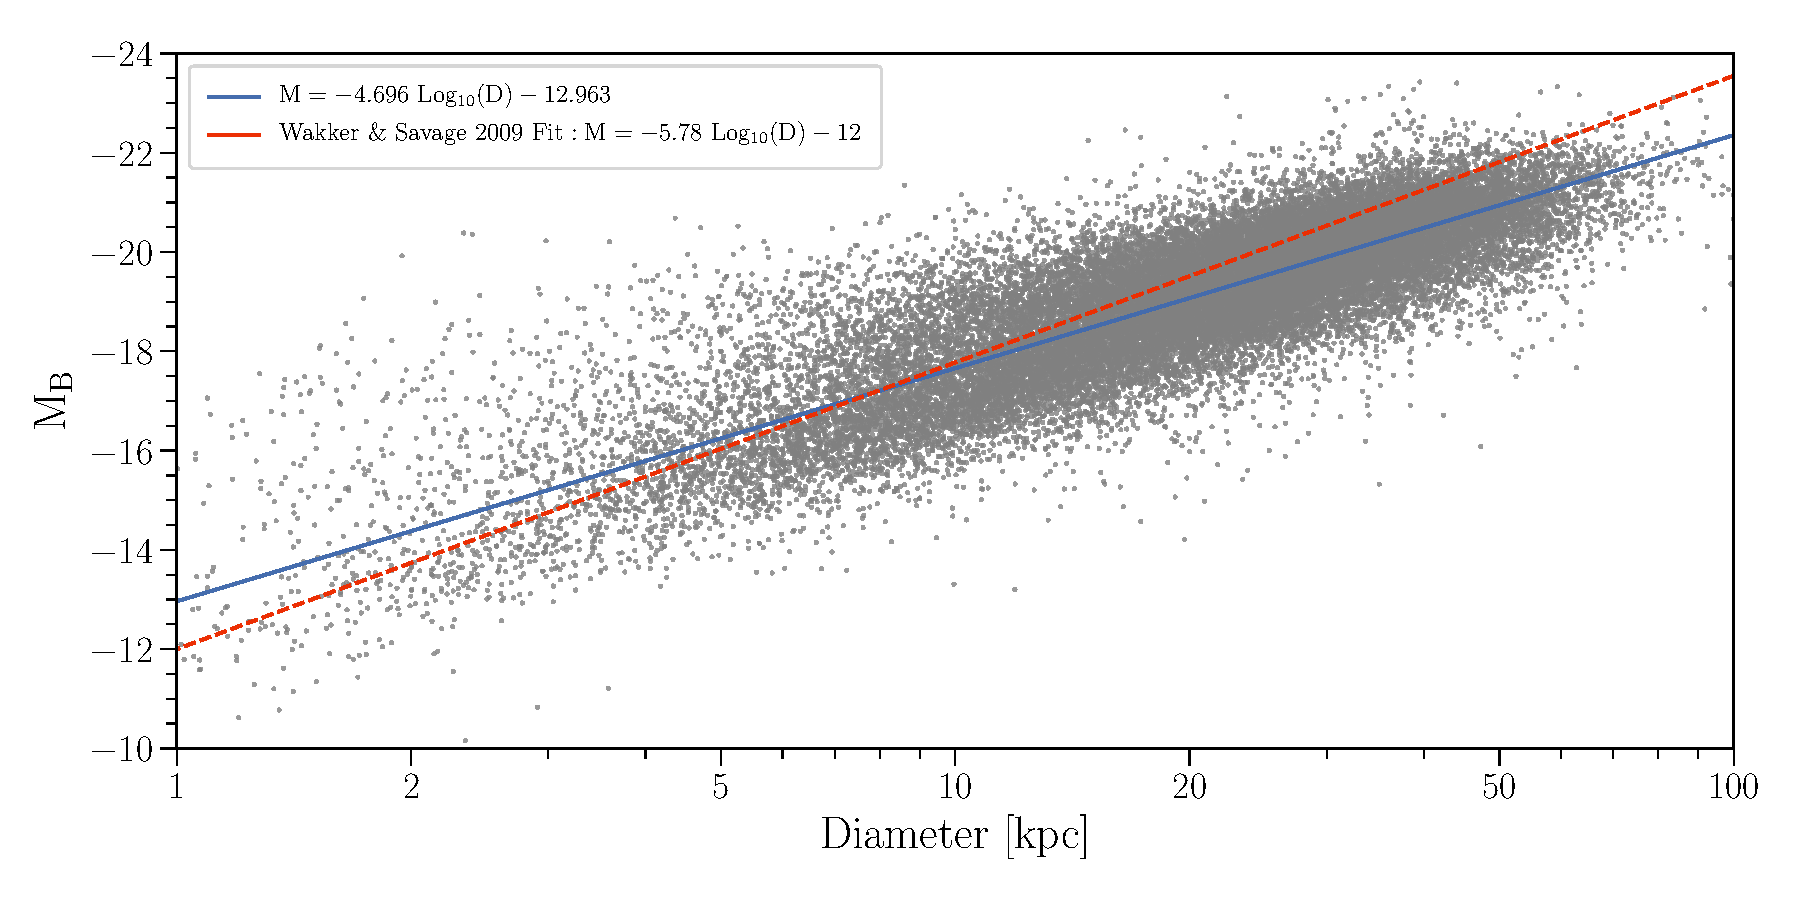
\includegraphics[width=0.99\textwidth]{Chap2/figures/mag_v_diam_fit2.pdf}
        \caption{\small{Relationship between absolute $B$-band magnitude and physical diameter for all galaxies with available data. Data are in grey, and a least-squares fit is shown in blue. The function form of this fit is $M ~=~ a ~ log_{10}(D) + b$, with fit parameters $a = -4.696 \pm 0.01$ and $b = -12.963 \pm 0.01$. We also include the fit derived by \cite{wakker2009} in dashed-red.}}
%        \vspace{-5pt}
        \label{magvdiam}
\end{figure}


\subsection{MinDiam\_ang} \label{MinDiam_ang}
Minor axis diameter in units of arcsec. See \ref{diameters} for a complete discussion.

\subsection{e\_MajDiam\_ang} \label{e_MinDiam_ang}
Major axis diameter error. This error is purely a result of the $1\sigma$ fit error to K\_s (2MASS) values, and thus does not take into account any observational errors.

\subsection{e\_MinDiam\_ang} \label{e_MinDiam_ang}
Minor axis diameter error. This error is purely a result of the $1\sigma$ fit error to K\_s (2MASS) values, and thus does not take into account any observational errors.

\subsection{MajDiam} \label{MajDiam}
Linear major axis diameter in units of kpc, calculated using $bestDist$. See \ref{diameters} for a complete discussion.

\subsection{MinDiam} \label{MinDiam}
Linear minor axis diameter in units of kpc, calculated using $bestDist$. See \ref{diameters} for a complete discussion.

\subsection{e\_MajDiam} \label{e_MajDiam}
Linear major axis diameter error. This error is purely a result of the $1\sigma$ fit error to K\_s (2MASS) values, and thus does not take into account any observational errors.

\subsection{e\_MinDiam} \label{e_MinDiam}
Linear minor axis diameter error. This error is purely a result of the $1\sigma$ fit error to K\_s (2MASS) values, and thus does not take into account any observational errors.

\subsection{R\_vir} \label{R_vir}
Virial radius estimate calculated as

\begin{equation}
log R_{vir} = 0.69 log D + 1.24.
\end{equation}

\noindent This follows the parametrization of \cite{stocke2013} relating a galaxy's luminosity to its virial radius, combined with the \cite{wakker2009} empirical relation between diameter and luminosity (see \citealt{wakker2015} and references therein for further details).

\subsection{inc} \label{inc}
Galaxy inclination calculated simply as $inc = \cos^{-1} (MinDiam / MajDiam)$ in units of degrees.

\subsection{adjustedInc} \label{adjustedInc}
Galaxy inclination calculated assuming a finite disk thickness following \cite{heidmann1972}:

\begin{equation}
	\cos(i) = \sqrt{\frac{q^2 - q_0^2}{1 - q_0^2}},
	\label{incEq}
\end{equation}

\noindent where $q$ is the ratio of minor to major axes and $q_0$ is the minimum disk thickness. We set $q_0 = 0.2$ for all galaxies. This value is a compromise, as some galaxies (e.g., Sc type) will have intrinsic $q_0$ closer to $\sim 0.13$, while highly bulged galaxies will have larger $q_0$ (e.g., see \citealt{heidmann1972c}). However, as morphologies are only available for a subset of galaxies, a generic inclination correction fits our need for homogeneity. The result is that very thin galaxies will be slightly biased towards higher inclination and vice-versa with thicker galaxies.

\subsection{e\_inc} \label{e_inc}
Inclination error derived from the error in major and minor axes fits (see \ref{diameters}). Measurement errors for diameters, axis-ratios, and position angles are inconsistently reported in NED, so this value only captures the additional error introduced by converting non-2MASS diameters. For consistency, we set 2MASS diameter errors uniformly at 5\%.

\subsection{PA} \label{PA}
Position angle in units of degrees. When multiple PA measurements are available for a given target, we choose the highest ranking measurement as outlined in \ref{diameters}.

\subsection{diam\_key} \label{diameter_key}
The chosen source of our diameter value. Published diameters are converted to an equivalent 2MASS $K_s$ ``total" value following the fits given in Table \ref{diameter_fits}.

\subsection{ratio\_key} \label{ratio_key}
The chosen source of our diameter axis-ratio value. This is used to calculate the minor axis diameters and inclinations (see Table \ref{diameter_fits}).

\subsection{pa\_key} \label{pa_key}
The chosen source of our position angle value (see Table \ref{diameter_fits}).

\subsection{RC3\_type} \label{RC3_type}
Galaxy morphology as published in the Third Reference Catalogue of Bright Galaxies (RC3; see Table 2 in Section 3.3.a, page 15, of the printed RC3; \citealt{RC3}). Galaxies not included in RC3 are marked `x'.

\subsection{RC3\_d25} \label{RC3_d25}
The RC3 apparent major isophotal diameter measured at the 25th magnitude surface-brightness level, in units of B-mag per arcsecond (see Section 3.4.a, page 21, of Volume I of the printed RC3; \citealt{RC3}).

\subsection{RC3\_r25} \label{RC3_r25}
The RC3 ratio of the major to minor axis isophotal diameter, converted from decimal logarithm to a straight ratio in order to match the units of $ratio\_key$ (see Section 3.4.b, page 26, of Volume I of the printed RC3; \citealt{RC3}).

\subsection{RC3\_pa} \label{RC3_pa}
The RC3 position angle in units of degrees (see Section 3.5.a, page 30, of Volume I of the printed RC3; \citealt{RC3}).

\subsection{group\_num} \label{group_num}
Group designation number taken from the \cite{tully2015} group catalogue.

\subsection{group\_mem} \label{group_mem}
Number of members in this galaxy group taken from the \cite{tully2015} group catalogue.

\subsection{group\_dist} \label{group_dist}
Distance to the galaxy group, taken from the \cite{tully2015} group catalogue.

\subsection{MType} \label{MType}
Morphological type as homogenized by NED. We have removed extraneous space characters, and then replaced the individual spaces with underscore characters.

\subsection{flag} \label{flag}
A flag to help identify suspected issues with a galaxy. For most objects $flag=0$. If, however, we suspect an object to be a star we set $flag=1$. Our criteria for this is as follows: 1) if an object has $Vhel < 500$ \kms, no diameter measurement, and no $MType$ available, 2) if $MType$ is found to match any of our exclude morphologies. Our full exclude list is the following: [`:', `0.9', `0.92', `14.247', `14.632', `14.728', `14.818', `14.998', `14', `15.159', `15.171', `15.242', `15.341', `15.458', `15.79', `15.819', `16.281', `16.309', `16.348', `16.394', `16.556', `16.736', `16.764', `16.783', `16.981', `16', `17.012', `17.039', `17.441', `17.597', `2\_compacts', `2\_or\_3?\_spirals', `2\_S0\_galaxies', `2\_S0\_pec\_galaxies', `2\_SB0?\_pec\_galaxies', `2\_Spec?', `2\_spirals', `2\_symm.sp.arms', `2E', `2MASS\_Extended\_Ver.2', `3\_S0\_galaxies', `A-star', `A', `A0', `A3\_HII', `AGN:', `AGN?', `AGN', `AGN+SF', `AGN1', `AGN2', `ALG', `Amorphous', `B...', `B', `bright\_near*', `Cand.\_glob.\_cluster', `Candidate\_AGN', `Candidate\_PN', `Carbon', `D', `DA-star', `DA:', `DA', `DA\_auto', `DA+M:;\_Cand.\_QSO', `DA+M:', `DA+M', `DANS?', `DANS?\_Sbrst', `DANS', `DANS\_WR?', `DBA', `DC:', `DGTO', `DISRPTD', `DISTRBD', `DQ;\_Cand.\_QSO', `DQ:', `DSa', `F', `F2', \\ `F6-F8;Candidate\_WD', `High\_vel.\_cloud', `K\_Star', `K1', `K4-K5;Candidate\_WD', `M', `M\_star', `M\_Star', `M0', `M0V', `M1', `M3-M4', `O', `Opt.var.', `Planetary, `Planetary?', `Planetary\_nebula', `PN:', `PN?', `Point\_Src\_[SDSS]', `Possible\_*Cl', `Possible\_star', `star:', `star??', `star?', `stellar-like', `stellar:', `stellar',\_or\_galaxy', `M-star']

%[`M-star', `M star', `Opt.var.', `K4-K5;Candidate WD', `F6-F8;Candidate WD', `A', `Candidate AGN', `M1', `star??', `O', `K Star', `PN?', `K1', `M0', `M0V', `A0', `DA-star', `High vel. cloud', `O', `Carbon', `Point Src [SDSS]', `Possible star', `Planetary nebula', `M3-M4', `F2', `A-star', `PN:', `Cand. glob. cluster', `Candidate PN', `F'].

Secondly, we set $flag = 2$ if the velocity implied by $RID\_median$ (i.e., $RID\_median$ * $H_{\rm 0}$) differs from $Vhel$ by more than 1500 \kms. If $flag = 2$, it may be wise to use $distvcorr$ instead of $bestDist$. There is no overlap between flag types, so no possible stars ($flag=1$) objects have a redshift-independent distance available.


\subsection{lumClass} \label{lumClass}
Luminosity class as assigned by NED. Roman numerals between I, II, III, IV, and V designate galaxies in order of decreasing luminosity in an analogous fashion to the standard stellar luminosity classes.

\subsection{E(B-V)} \label{E(B-V)}
Galactic mean dust extinction in the direction of each galaxy from \cite{schlafly2011}.\footnote{See \url{https://irsa.ipac.caltech.edu/applications/DUST/}}
%Schlafly and Finkbeiner (2011)


\subsection{Bmag} \label{Bmag}
The median B-band magnitude. For each galaxy we retrieved all $B$-band and SDSS $g$, $r$, and $z$ measurements. Direct $B$-band measurements are available for $\sim 30\%$ of galaxies, and a large fraction of the remaining objects have SDSS magnitudes. We convert SDSS magnitudes to $B$-band via $B = g + 0.39 (g-r) + 0.21$ \citep{jester2005}. Per SDSS DR12 guidelines, we preferentially selected SDSS $petrosian$ magnitudes when available, followed by $model$ and $cmodel$ values if $petrosian$ was not available. We then selected the min, max and median $B$-band values when more than one was available for inclusion in the final data product. SDSS-converted $B$-band values are included as a separate estimate ($Bmag\_sdss$; \S \ref{Bmag_sdss}). 

\subsection{Bmag\_key} \label{Bmag_key}
The name of the source or catalog responsible for producing our chosen value of $Bmag$.

\subsection{Bmag\_max}
The brightest B-band magnitude available in NED for this object. See \ref{Bmag} for details.

\subsection{Bmag\_max\_key}
The name of the source or catalog responsible for producing $Bmag\_max$.

\subsection{Bmag\_min}
The dimmest B-band magnitude available in NED for this object. See \ref{Bmag} for details.

\subsection{Bmag\_min\_key}
The name of the source or catalog responsible for producing $Bmag\_min$.

\subsection{Bmag\_sdss} \label{Bmag_sdss}
SDSS $g$ and $r$-band measurements converted to $B$-band via $B = g + 0.39 (g-r) + 0.21$ \citep{jester2005}. See \ref{Bmag} for details.

\subsection{gmag\_sdss}
SDSS $g$-band magnitude. This value is used in the $Bmag\_sdss$ calculation (see \S \ref{Bmag}).

\subsection{rmag\_sdss}
SDSS $r$-band magnitude. This value is used in the $Bmag\_sdss$ calculation (see \S \ref{Bmag}).

\subsection{zmag\_sdss}
SDSS $z$-band magnitude (see \S \ref{Bmag}).

\subsection{Lstar\_med} \label{Lstar_med}
The $L / $\Lstar ratio calculated using $Bmag$ and $bestDist$. We compute luminosity in units of \Lstar for each of the min, median, max and SDSS $B$-band values as follows:

\begin{equation}
	\frac{L}{L^*} = 10^{-0.4 (M_{\rm B} - M_{\rm B^{*}})},
	\label{lstar}
\end{equation}

\noindent where $M_{\rm B}$ is the galaxy absolute magnitude, calculated using the $bestDist$ distance estimate as described above. We adopted the CfA galaxy luminosity function by \citep{marzke1994}, which sets $B^{*} $ = -19.57. 


\subsection{e\_Lstar\_med} \label{e_Lstar_med}
$Lstar\_med$ error calculated with $e\_Bmag$ and $e\_bestDist$. Combining these errors leads to the following error formula:

\begin{equation}
	e\_Lstar\_med = 0.921 \sqrt{10^{-0.8(M - M^*)}  \Delta M^2},
\end{equation}
\noindent where $\Delta m$ is the error in $Bmag$.

%Errors from $E(B-V)$ are relatively negligible and thus were not included.


\subsection{Lstar\_max}
The $L / $\Lstar  ratio calculated using $B\_max$ and $bestDist$ + $e\_bestDist$ following Eq. \ref{lstar}. \\


\subsection{e\_Lstar\_max}
$Lstar\_max$ error calculated with $e\_Bmag\_max$ and $e\_bestDist$ (see \S \ref{e_Lstar_med}).


\subsection{Lstar\_min}
The $L / $\Lstar ratio calculated using $B\_min$ and $bestDist$ - $e\_bestDist$ following Eq. \ref{lstar}.


\subsection{e\_Lstar\_min}
$Lstar\_min$ error calculated with $e\_Bmag\_min$ and $e\_bestDist$ (see \S \ref{e_Lstar_med}).


\subsection{Lstar\_sdss}
The $L / $\Lstar ratio calculated using $Bmag\_sdss$ and $bestDist$ following Eq. \ref{lstar}.


\subsection{e\_Lstar\_sdss}
$Lstar\_sdss$ error calculated with $e\_bestDist$ and \cite{jester2005} conversion errors (see \S \ref{e_Lstar_med}).


\subsection{altNames}
The NED list of alternative object names for this galaxy with spaces removed. In the main catalogue we have included only NGC, IC, UGC, SDSS, and 2MASS names in this column. The associated alternative names catalogue contains the full list. Note that our preferred name, $Name$, and $NEDname$ will only appear in the $altNames$ list if they match these same criteria.\\


\section{Limitations \& Future}

This catalogue is not meant to be entirely robust or comprehensive - rather it's purpose is to present a common batch of parameters for nearby galaxies in a easily retrievable and machine-readable manner. We have nonetheless endeavored to provide reasonable error estimates on all derivations and for as many observed quantities as possible.

Some caveats:

\begin{enumerate}

\item{This is not the result of a targeted survey or observing program, so it's coverage and completeness is inherently non-uniform. We have endeavored to quantify this non-uniformity in Section \ref{completeness}. A future version of this catalogue will include all-sky coverage maps for each relevant major input catalog (e.g., SDSS, 2MASS, etc.).}

\item{The quality of the data and observational errors are difficult to determine. We present this dataset as more of a convenient "quick-look" directory than a scientifically rigorous data product.}

\item{This catalogue will soon be made available online as a searchable SQL database, and downloadable in csv and ascii-fixed-width formats. Please contact the authors for details.}
\end{enumerate}


\acknowledgements

This research has made use of the NASA/IPAC Extragalactic Database (NED) which is operated by the Jet Propulsion Laboratory, California Institute of Technology, under contract with the National Aeronautics and Space Administration. 

%Based on observations with the NASA/ESA \textit{Hubble Space Telescope}, obtained at the Space Telescope Institute, which is operated by AURA, Inc., under NASA contract NAS 5-26555.

%\nocite{*}
\bibliographystyle{thesis}
%\bibliography{/Users/clairemurray/Desktop/DMF_thesis/bib}
\bibliography{/Users/frenchd/Research/inclination/git_inclination/thesis/DMF_thesis/bib}





\chapter[Probing Large Galaxy Halos at $z\sim0$ with Automated $\rm Ly\alpha$-Absorption Matching]{Probing Large Galaxy Halos at $z\sim0$ with Automated $\rm L \MakeLowercase{y} \alpha$-Absorption Matching} 
\label{chap:chap3}

% Leave space between title and quote or publication note.  This has often been
% 10cm for a quote and 8 cm for a reference, but this is really up to you.
%\vspace{8cm}

\vfill


\begin{flushright}
    \fixspacing % Single spacing
    \textit{A version of this chapter has previously appeared\\
        in the \emph{Astrophysical Journal}} \\ \vspace{1ex}
     D.\,M. French \& B.\,P. Wakker, 2017, \apj, 837, 2
\end{flushright}

\vspace*{1in} % Leave a 1-in space at the bottom.

\cleardoublepage


\begin{chabstract}

We present initial results from an ongoing large-scale study of the circumgalactic medium in the nearby Universe ($cz \leq 10,000$ $\rm km\, s^{-1}$), using archival Cosmic Origins Spectrograph spectra of background quasi-stellar objects. This initial sample contains 33 sightlines chosen for their proximity to large galaxies ($D\geq25$ kpc) and high signal-to-noise ratios (S/N $\geq$ 10), yielding 48 Ly$\alpha$ absorption lines that we have paired with 33 unique galaxies, with 29 cases where multiple absorbers within a single sightline are paired with the same galaxy. We introduce a likelihood parameter to facilitate the matching of galaxies to absorption lines in a reproducible manner. We find the usual anti-correlation between Ly$\alpha$ equivalent width ($EW$) and impact parameter ($\rho$) when we normalize by galaxy virial radius ($R_{\rm vir}$). Galaxies associated with a Ly$\alpha$ absorber are found to be more highly-inclined than galaxies in the survey volume at a $>99\%$ confidence level (equivalent to $\sim 3.6 \sigma$ for a normal distribution). In contrast with suggestions in other recent papers of a correlation with azimuth angle for Mg\,{\sc ii} absorption, we find no such correlation for Ly$\alpha$.

\end{chabstract}


%\keywords{galaxies:intergalactic medium, galaxies:evolution, galaxies:halos, quasars: absorption lines}


\section{Introduction}

It is well known that galaxies must continue to accrete gas throughout their lifetimes in order to sustain their observed levels of star formation (e.g., Erb 2008; Prochaska $\&$ Wolfe 2009; Putman et al. 2009a, 2009b; Bauermeister et al. 2010; Genzel et al. 2010). This additional gas must come from the diffuse intergalactic medium (IGM), where the majority of the baryons in the universe reside (Penton et al. 2002, 2004; Lehner et al. 2007; Danforth $\&$ Shull 2008; Shull et al. 2012). How exactly this IGM gas eventually falls into the halos and disks of galaxies is still highly uncertain, as observational constraints are hard to come by. Because of the diffuse nature of IGM gas, it is most readily and sensitively detected as absorption in the spectra of background quasi-stellar objects (QSOs). The advent of the sensitive ultraviolet (UV) Cosmic Origins Spectrograph (COS) on the \textit{Hubble Space Telescope} (\textit{HST}; Osterman et al. 2011; Green et al. 2012) has provided a wealth of information about the properties and distribution of both the ions of heavy elements as well as the Lyman series of neutral hydrogen (H\,{\sc i}) gas around galaxies. 

Individual concentrations of gas along a given sightline imprint absorption lines onto the spectrum in the direction of the QSO. The metal lines trace the star formation history within the intervening gas, and H\,{\sc i} lines (e.g., Ly$\alpha$) indicate both the location and velocities of outflowing gas, as well as the presence of fuel for future star formation. Numerous studies using these observations have shown that many Ly$\alpha$ absorbers trace individual galaxy halos (e.g., Lanzetta et al 1995; Chen et al. 1998, 2001; Tripp et al. 1998; Wakker $\&$ Savage 2009; Steidel et al. 2010; Prochaska et al. 2011; Tumlinson et al. 2011, 2013; Thom et al. 2012;  Stocke et al. 2013, 2014; Liang $\&$ Chen 2014; Tejos et al. 2014; Borthakur et al. 2015).

Some recent studies found that about half of Ly$\alpha$ absorbers lie within galaxy halos, at impact parameters $\rho<350$ kpc (C\^{o}t\'{e} et al. 2005; Prochaska et al. 2006; Wakker $\&$ Savage 2009). In addition, Wakker $\&$ Savage (2009) found that an absorber lies within 400 kpc and 400 $\rm km\, s^{-1}$ for $90\%$ of galaxies brighter than $0.1$\Lstar, and all galaxies have a Ly$\alpha$ absorber within 1.5 Mpc. Higher-redshift studies, such as Rudie et al. (2012a) at $2<z<3$, found evidence for an elevated density of absorbers up to 2 Mpc from galaxies. Wakker $\&$ Savage (2009) also discovered a correlation between Ly$\alpha$ absorption linewidth and impact parameter $\rho$, observing that the broadest lines (FWHM $>$150 $\rm km\, s^{-1}$) are only seen within 350 kpc of a galaxy, while at $\rho>1$ Mpc, only lines with FWHM $<75$ $\rm km\, s^{-1}$ occur. This suggests that the temperature and/or turbulence of gas increases in the presence of galaxies, a hypothesis that has been further supported by the results of Wakker et al. (2015). 

Studying the enrichment of galaxy halos is necessary for constraining outflow models and informing stellar feedback prescriptions. Directly measuring the velocities and column densities of absorbers as a function of impact parameter and orientation around galaxies would provide the clearest evidence of inflow or outflow activity, but results are still uncertain. Kacprzak et al. (2011b) claimed to find that Mg\,{\sc ii} equivalent widths correlate with galaxy inclination, but Mathes et al. (2014) found no such correlation for Ly$\alpha$ and O\,{\sc vi} absorbers. Furthermore, we should expect outflowing gas to be more highly enriched and trace the metallicity of the associated galaxy, with inflowing gas instead appearing only in H\,{\sc i}. Both Stocke et al. (2013) and Liang $\&$ Chen (2014) found an ``edge'' to heavy ion absorption at $\sim0.5R_{\rm vir}$, but found Ly$\alpha$ covering fractions of $\sim0.75-1$ continuing out to $R_{\rm vir}$. However, Mathes et al. (2014) measured O\,{\sc vi} absorption out to $\sim3 R_{\rm vir}$, and Savage et al. (2014) found that more than half of O\,{\sc vi} absorption occurs beyond 1 $R_{\rm vir}$ from the nearest galaxy. Additionally, Borthakur et al. (2015) found that Ly$\alpha$ absorption $EW$ correlates with galaxy H\,{\sc i} gas fraction, but only weakly with SFR, suggesting that accretion flow from the CGM is slow and continuous.

Recent results from Kacprzak et al. (2011b, 2012a) suggest that absorbing systems have a preferred orientation with respect to the major and minor axes of the galaxies they are associated with. This could be evidence of inflows and outflows, or an effect of the global structure of galaxy halos, but the statistics are not yet good enough to provide consistent answers. A larger-scale study of inclination and azimuthal angles versus absorber properties is needed in order to elucidate the distribution of absorbing systems around galaxies. This is most easily done for the largest galaxies in the nearby universe, where it is possible to obtain inclinations and unambiguous absorber associations. 

Previous studies have suffered from small sample sizes (e.g., Mathes et al. 2014 used 14 galaxies, Stocke et al. 2013 used 11, Werk et al. 2014 used 44), incompleteness due to their higher mean redshifts (e.g., the Mathes et al. 2014 sample is $0.12 <z<0.67$), and limited impact parameter reach (e.g., Werk et al. 2014 probed CGM gas only within $\rho < 160$ kpc of galaxies). To address these shortcomings, we are conducting a large survey of the properties of intergalactic gas in the nearby universe, where we have good and relatively complete information on both faint and bright galaxies, in order to reveal how the IGM and galaxies affect each other. 

We are taking advantage of the over 500 archived QSO and Seyfert spectra taken by the COS and Space Telescope Imaging Spectrograph (STIS) on \textit{HST}, combined with the wealth of information available for the $\sim100,000$ galaxies with $cz<10,000$ $\rm km\, s^{-1}$ found in the NASA Extragalactic Database (NED) to probe the environment of absorbing gas systems in the nearby universe. In this paper we introduce a new, numerical method for associating absorption lines with nearby galaxies. This approach will allow for an objective understanding of the distribution of the gas around galaxies, which requires looking for both detections and non-detections of gas, both near and far from galaxies, with a robust and reproducible metric for matching galaxies with absorption.

This paper presents our likelihood-matching method with initial results from a pilot study of 33 sight lines, chosen for their proximity to large galaxies and high signal-to-noise spectra. It is organized as follows. In Section 2 we present the data and analysis techniques, in Section 3 we present the results, in Section 4 we discuss possible interpretations of our results, and in Section 5 we present a summary.


%\begin{table}[ht]
%\caption{\small{COS Targets in this Sample}}
%  \vspace{-15pt}
%\begin{center}
%\begin{tabular}{l l l l l l l l l l}
% \hline \hline
%  Target 					& R.A. 		& Decl. 		 & \textit{z}	  & Program 	  & Grating 	   & Obs ID 	    & Obs Date 	     & $\rm T_{exp}^a$     & $\rm S/N^a$  \\ 
%  	    					& 	       		&	  		 & 		  	  & 		    	  & 		  	   & 		  	    & 		     	     & 	        [ks]         & [1238] \\ 
% \scriptsize (1)  				& \scriptsize (2) & \scriptsize (3) & \scriptsize (4) & \scriptsize (5) & \scriptsize (6) & \scriptsize  (7) & \scriptsize (8) & \scriptsize (9) & \scriptsize (10)  \\ \hline \hline
%\\
%    
%1H0717+714		  		&  07 21 53.3  &  +71 20  36	&    0.5003	& 12025	&   G130M	&   LBG812	& 11-12-27      	 	  &  6.0    &      37         \\
%2dFGRS\_S393Z082  		&  02 45 00.8  &  $-$30 07  23	&    0.3392	& 12988	&   G130M	&   LC1040	& 13-05-27,28 	 	  & 17.7   &      10         \\
%				  		&		       &			&			&		&			&    LC1045	&				  &	       &		   \\
%FBQSJ1431+2442     		&  14 31 25.8  &  +24 42 20	&   0.4069		& 13342	&   G130M	&   LC8903	& 15-03-29		  & 16.5  &      17          \\
%				 		&		       &			&			& 12603	&			&   LBS314	& 13-03-08		  &	      &		  	  \\
%H1101-232   		 		&  11 03 37.7  &  $-$23 29 31	&   0.1860		& 12025	&   G130M	&   LBG804	& 11-07-05  		   & 13.3  &      16         \\
%HE0241-3043  		 		&  02 43 37.7  &  $-$30 30 48	&   0.6693		& 12988	&   G130M	&   LC1070	& 13-06-21  		   & 7.0    &      14         \\
%LBQS1230-0015  	 		&  12 33 04.1  &  $-$00 31 34    	&   0.4709		& 11598	&   G130M	&   LB5N15	& 10-08-01  		   & 10.3  &      13         \\
%				 		&		       &			&			& 12486	&			&   LBP250	& 12-04-26		   &	       &	  	   \\
%MRC2251-178  	 		&  22 54 05.9  &  $-$17 34 55	&   0.0661		& 12029	&   G130M	&   LBGB03	& 11-09-29                   &  5.5   &      42         \\
%Mrk290  					&  15 35 52.3  &  +57 54 09	&   0.0296		& 11524	&   G130M	&   LB4Q02	& 09-10-28  		   &   3.9  &      38         \\
%Mrk876  					&  16 13 57.2  &  +65 43 10	&   0.1290		& 11524	&   G130M	&   LB4Q03	& 10-04-08,09  		   & 12.6  &      65         \\
%				 		&		       &			&			& 11686	&			&   LB4F05	&				   &	       &	  	   \\
%Mrk1014  					&  01 59 50.2  &  +00 23 41	&   0.1630		& 12569	&   G130M	&   LBP404	& 12-01-25  		   &  1.8   &      17         \\
%PG0832+251  				&  08 35 35.9  &  +24 59 41	&   0.3310		& 12025	&   G130M	&   LBG808	& 12-04-19		   &  6.1   &      14         \\
%PG0003+158  				&  00 05 59.3  &  +16 09 49	&   0.4509		& 12038	&   G130M	&   LBGL17	& 11-10-22  		   & 10.4  &      25         \\
%PG1001+054  				&  10 04 20.1  &  +05 13 01	&   0.1610		& 13347	&   G130M	&   LCCV02	& 14-06-19  		   &  5.2   &      14         \\
%						&		       &			&		 	& 13423	&			&   LC9W02	& 14-04-04		   &	       &	  	   \\
%PG1302-102  				&  13 05 33.0  &  $-$10 33 20	&   0.2784  	& 12038	&   G130M	&   LBGL04	& 11-08-16  		   &  6.0   &      27         \\
%RBS1768  				&  21 38 49.7  &  $-$38 28 40	&   0.1830  	& 12936	&   G130M	&   LC1201	& 13-06-25		   &  7.0   &      24         \\
%RX J0714.5+7408  			&  07 14 36.2  &  +74 08 11	&   0.3710  	& 12275	&   G130M	&   LBH402	& 11-03-18   		   &  8.3   &      18         \\
%RX J1017.5+4702  			&  10 17 30.9  &  +47 02 25	&   0.3354  	& 13314	&   G130M	&   LC9M04	& 14-01-29		   &  8.7   &      12         \\
%RX J1117.6+5301  			&  11 17 40.5  &  +53 01 50	&   0.1587  	& 14240	&   G130M	&   LCWM05	& 16-04-13		   &  4.9   &      11         \\
%RX J1236.0+2641  			&  12 36 04.1  &  +26 41 36	&   0.2092  	& 12248	&   G130M	&   LBH087	& 12-01-29  		   &  4.2   &      11         \\
%RX J1330.8+3119  			&  13 30 53.2  &  +31 19 32	&   0.2423  	& 12248	&   G130M	&   LBHO85	& 11-07-11		   &   4.3  &      11         \\
%RX J1356.4+2515  			&  13 56 25.6  &  +25 15 23	&   0.1640  	& 12248	&   G130M	&   LBH057	& 12-02-03		   &   2.3  &      10         \\
%RX J1503.2+6810  			&  15 03 16.5  &  +68 10 06	&   0.1140  	& 12276	&   G130M	&   LBI609		& 10-12-31 		   &   1.9  &      11         \\
%RX J1544.5+2827  			&  15 44 30.5  &  +28 27 56	&   0.2314  	& 13423	&   G130M	&   LC9W08	& 14-02-25		   &   2.1  &      10         \\
%RX J2043.1+0324  			&  20 43 06.2  &  +03 24 50	&   0.2710  	& 13840	&   G130M	&   LCJW02	& 14-10-23		   &   7.8  &      15         \\
%RX J2139.7+0246  			&  21 39 44.2  &  +02 46 05	&   0.2600  	& 13840	&   G130M	&   LCJW03	& 14-10-27  		   & 	7.9  &      16         \\
%SBS0957+599         			&  10 01 02.6  &  +59 44 15	&   0.7475  	& 12248	&   G130M	&   LBHO65	& 11-03-18,19  		   &   3.3  &      12         \\
%SDSSJ021218.32-073719.8  	&  02 12 18.3  &  $-$07 37 20	&   0.1739  	& 12248	&   G130M	&   LBHO83	& 11-06-26		   &   6.5  &      12         \\
%				        	     	& 	  	       &			&    	  	 	&		&			&   LBHO92	& 11-08-21		   &          &                   \\
%				        	     	& 	               &			&    	  	 	&		&			&   LBHO92	& 11-08-21		   &          &                   \\
%SDSSJ080838.80+051440.0 	&  08 08 38.8  &  +05 14 40	&   0.3606  	& 12603	&   G130M	&   LBS330	& 12-03-17  		   &   4.7  &      10         \\
%SDSSJ091728.60+271951.0 	&  09 17 28.6  &  +27 19 51	&   0.0756  	& 14071	&   G130M	&   LCX202	& 15-11-30		   & 15.5  &      11         \\
%				        	     	& 	  	      &				&    	  	 	&		&			&   LCX2Z2	& 16-02-06		   &          &                   \\
%SDSSJ112224.10+031802.0 	&  11 22 24.1  &  +03 18 02	&   0.4753  	& 12603	&   G130M	&   LBS318	& 13-03-29		   &   7.6  &      13         \\
%SDSSJ130524.30+035731.0 	&  13 05 24.3  &  +03 57 31	&   0.5457  	& 12603	&   G130M	&   LBS321	& 12-06-25,26		   &   7.6  &      13         \\
%SDSSJ135726.27+043541.4 	&  13 57 26.2  &  +04 35 41	&   1.2345  	& 12264	&   G130M	&   LBJ005	& 11-06-22		   & 14.1  &      21         \\
%				        	     	& 	  	      &				&    	  	 	&		&			&   LBJ007	& 11-06-26		   &          &                   \\
%SDSSJ140428.30+335342.0 	&  14 04 28.3  &  +33 53 42	&   0.5500  	& 12603	&   G130M	&  LBS320	& 13-03-03   		   &   7.7  &      10          \\
%TON1009  			    	&  09 09 06.1  &  +32 36 31	&   0.8103  	& 12603	&   G130M	&  LBS328	& 12-04-22   		   &   4.7  &      12         \\
% \\
%\hline
%\end{tabular}
%
%\footnotesize \raggedright \textbf{Note.}\\
%\footnotesize \raggedright $^{\rm a}$ Total exposure time and S/N ratio is given for multi-orbit exposures. \\
%\end{center}
%  \label{table1}
%\end{table}

\section{Data and Analysis}

\subsection{Galaxy Data}
Achieving the goal of this study relies on knowing the locations and properties of all galaxies near detected Ly$\alpha$ absorption lines. To facilitate this, we have constructed a database of all $z\leq 0.033$ ($cz\leq 10,000$ $\rm km\, s^{-1}$) galaxies with published data available through the NASA Extragalactic Database (NED). A full description of this catalog will be presented in D. M. French $\&$ B. P. Wakker (2017, in preparation). Here we summarize its most important aspects.

\begin{figure}[b!]
        \centering
        \vspace{0pt}
        \includegraphics[width=0.50\textwidth]{Chap3/figures/fig1.pdf}
        \caption{\small{Distribution of $L/$\Lstar~ values for all galaxies in the dataset. The red dashed vertical lines highlight 1, 0.5, 0.1, 0.05 and 0.01 \Lstar.}}
        \label{completeness}
\end{figure} 

The galaxy data set contains over 108,000 entries, and includes data from SDSS, 2MASS, 2dF, 6dF, RC3, and many other, smaller surveys. Our criterion for including a galaxy in this data set is only an accurate, spectroscopic redshift that places the galaxy in the $cz \leq 10,000$ $\rm km\, s^{-1}$ velocity range. This restriction leads to a completeness limit of $B \lesssim 18.7$ mag, or $\sim0.2 $\Lstar, at $cz = 10,000$ $\rm km\, s^{-1}$, and progressively better towards lower velocities (see Figure \ref{completeness}). 

This limit will vary depending on which major surveys include a particular region of the sky. The major contributor is whether or not SDSS data are available, which begins around $cz = 5000$ $\rm km\, s^{-1}$. Figure \ref{completeness} is split into four velocity bins to illustrate this. Our data are complete down to $\sim0.1$\Lstar~ in the first bin, $0 \leq cz \leq 2500$ $\rm km\, s^{-1}$. At slightly higher velocities, $2500 \leq cz \leq 6000$ $\rm km\, s^{-1}$, the completeness falls to barely better than $\sim1.0$\Lstar~ as we move past the near and well studied galaxies, but have yet to reach the footprint of deep surveys. SDSS data become available in the last two bins, spanning $6000 \leq cz \leq 10,000$ $\rm km\, s^{-1}$. While the $8000 \leq cz \leq 10,000$ $\rm km\, s^{-1}$ region appears to reach the expected SDSS limits of $B \lesssim 18.7$ mag, or $\sim0.2$\Lstar, the $6000 \leq cz \leq 8000$ $\rm km\, s^{-1}$ region instead appears to flatten below $\sim 1.0$\Lstar. It is possible this is due to larger distance errors, since in this region redshift-independent distances are rare, and Hubble flow distances are still small enough to remain relatively uncertain.

Additionally, we have homogenized the galaxy data beyond the steps taken by NED by normalizing all measurements of galaxy inclination, position angle, and diameter to 2MASS $K$-band values. Most galaxies in NED have measures of inclination, position angle and diameter available in several different bands, so in order to make meaningful comparisons it is necessary to automatically choose one band for all measurements. We chose 2MASS values for this because it was an all-sky survey, and represents the largest fraction of available galaxy data. Physical galaxy diameters are derived from 2MASS $K_{s}$ ``total" angular diameter measurements and galaxy distances. 2MASS $K_{s}$ ``total" diameter estimates are surface brightness extrapolation measurements and are derived as 

\begin{equation}
	r_{\rm tot} = r' + a(\ln(148)^b,
\end{equation}

\noindent where $r_{tot}$ is defined as the point where the surface brightness extends to 5 disk scale lengths, $r'$ is the starting point radius ($>5" - 10"$ beyond the nucleus, or core influence), and $a$ and $b$ are Sersic exponential function scale length parameters ($f = f_0 \exp{(-r/a)}^{(1/b)}$; see Jarrett et al. 2003 for a full description). Approximately $50\%$ of all the galaxies have this 2MASS $K_{s}$ ``total" diameter. Of the remainder, $20\%$ have SDSS diameters, $27\%$ have no published diameter, and $3\%$ have diameters from other surveys. We convert values in these other bands to 2MASS $K_{s}$ ``total" diameters via a simple least squares linear fit when necessary.

We used $B$-band magnitudes to estimate each galaxy's luminosity in units of \Lstar~ as follows:

\begin{equation}
	\frac{L}{L^*} = 10^{-0.4 (M_{\rm B} - M_{\rm B^{*}})}.
\end{equation}

We adopt the CfA galaxy luminosity function by Marzke et al. (1994), which sets $B^{*} $ = -19.57. Direct $B$-band measurements are available for $\sim 30\%$ of galaxies, and most of the rest have SDSS $g$ and $r$ magnitudes, which can be converted to $B$ via $B = g + 0.39 (g-r) + 0.21$ (Jester et al. 2005). Finally, we also compute an estimate of the virial radius of each galaxy as $\log R_{\rm vir} = 0.69 \log D + 1.24$. This follows the parametrization of Stocke et al. (2013) relating a galaxy's luminosity to its virial radius, and the Wakker $\&$ Savage (2009) empirical relation between diameter and luminosity (see Wakker et al. 2015 and references therein for further details). Errors are propagated from the original published magnitude errors.

This homogeneous galaxy data table allows us to draw direct comparisons between the properties of the absorbers and the properties, separations, and environments of nearby galaxies with unprecedented completeness. The full dataset will be publicly released and discussed in further detail in a forthcoming paper (D. M. French $\&$ B. P. Wakker 2017, in preparation).


\subsection{Spectra}

This initial pilot study contains 33 sightlines to bright QSOs observed with COS. We chose sightlines by first sorting the galaxy data table described above by galaxy diameter. This sorted list is then correlated with the full list of publicly available sightlines, and only those systems with impact parameters less than 500 Mpc and galaxy diameters, $D$, greater than $25$ kpc, are kept. Finally, we select 33 sightlines with $S/N \geq 10$ from this list (see Table \ref{table1}).

All COS spectra for the target sightlines were obtained through the Barbara A. Mikulski Archive for Space Telescopes (MAST), and processed with CALCOS v3.0 or later. We combined individual exposures by the method of Wakker et al. (2015), which
\begin{landscape}

% Change the footnote style to lowercase letters
\renewcommand{\thefootnote}{\alph{footnote}}

\scriptsize
\begin{center}
\begin{longtable}{l l l l l l l l l l}
\caption[Pilot Sample: COS Targets]{COS Targets in this Sample} \label{table1} \\

\hline \hline \\[-2ex]
  \multicolumn{1}{c}{Target} & 
  \multicolumn{1}{c}{R.A.} &
  \multicolumn{1}{c}{Decl.} &
  \multicolumn{1}{c}{\textit{z}} &
  \multicolumn{1}{c}{Program} &
  \multicolumn{1}{c}{Grating} &
  \multicolumn{1}{c}{Obs ID} &
  \multicolumn{1}{c}{Obs Date} &
  \multicolumn{1}{c}{$\rm T_{exp}$\tablenotemark{a}} &
  \multicolumn{1}{c}{$\rm S/N^a$}  \\
  
  % Units
  \multicolumn{1}{c}{} & 
  \multicolumn{1}{c}{} &
  \multicolumn{1}{c}{} &
  \multicolumn{1}{c}{} &
  \multicolumn{1}{c}{} &
  \multicolumn{1}{c}{} &
  \multicolumn{1}{c}{} &
  \multicolumn{1}{c}{} &
  \multicolumn{1}{c}{(ks)} &
  \multicolumn{1}{c}{(1238)} \\
  
  % column numbers
  \multicolumn{1}{c}{(1)} & 
  \multicolumn{1}{c}{(2)} &
  \multicolumn{1}{c}{(3)} &
  \multicolumn{1}{c}{(4)} &
  \multicolumn{1}{c}{(5)} &
  \multicolumn{1}{c}{(6)} &
  \multicolumn{1}{c}{(7)} &
  \multicolumn{1}{c}{(8)} &
  \multicolumn{1}{c}{(9)} &
  \multicolumn{1}{c}{(10)} \\[0.5ex] \hline \\[-1.8ex]
\endfirsthead

% Second page
\multicolumn{10}{c}{{\tablename} \thetable{} -- Continued} \\[0.5ex]
\hline \hline \\[-2ex]
  \multicolumn{1}{c}{Target} & 
  \multicolumn{1}{c}{R.A.} &
  \multicolumn{1}{c}{Decl.} &
  \multicolumn{1}{c}{\textit{z}} &
  \multicolumn{1}{c}{Program} &
  \multicolumn{1}{c}{Grating} &
  \multicolumn{1}{c}{Obs ID} &
  \multicolumn{1}{c}{Obs Date} &
  \multicolumn{1}{c}{$\rm T_{exp}$\tablenotemark{a}} &
  \multicolumn{1}{c}{$\rm S/N^a$}  \\
  
  % Units
  \multicolumn{1}{c}{} & 
  \multicolumn{1}{c}{} &
  \multicolumn{1}{c}{} &
  \multicolumn{1}{c}{} &
  \multicolumn{1}{c}{} &
  \multicolumn{1}{c}{} &
  \multicolumn{1}{c}{} &
  \multicolumn{1}{c}{} &
  \multicolumn{1}{c}{(ks)} &
  \multicolumn{1}{c}{(1238)} \\
  
  % column numbers
  \multicolumn{1}{c}{(1)} & 
  \multicolumn{1}{c}{(2)} &
  \multicolumn{1}{c}{(3)} &
  \multicolumn{1}{c}{(4)} &
  \multicolumn{1}{c}{(5)} &
  \multicolumn{1}{c}{(6)} &
  \multicolumn{1}{c}{(7)} &
  \multicolumn{1}{c}{(8)} &
  \multicolumn{1}{c}{(9)} &
  \multicolumn{1}{c}{(10)} \\[0.5ex] \hline \\[-1.8ex]
  \endhead

\multicolumn{10}{l}{{Continued on Next Page\ldots}} \\
\endfoot

\\[-1.8ex] \hline \hline
\endlastfoot

%Data starts here:
1H0717+714		  		&  07 21 53.3  &  +71 20  36	&    0.5003	& 12025	&   G130M	&   LBG812	& 11-12-27      	 	  &  6.0    &      37         \\
2dFGRS\_S393Z082  		&  02 45 00.8  &  $-$30 07  23	&    0.3392	& 12988	&   G130M	&   LC1040	& 13-05-27,28 	 	  & 17.7   &      10         \\
				  		&		       &			&			&		&			&    LC1045	&				  &	       &		   \\
FBQSJ1431+2442     		&  14 31 25.8  &  +24 42 20	&   0.4069		& 13342	&   G130M	&   LC8903	& 15-03-29		  & 16.5  &      17          \\
				 		&		       &			&			& 12603	&			&   LBS314	& 13-03-08		  &	      &		  	  \\
H1101-232   		 		&  11 03 37.7  &  $-$23 29 31	&   0.1860		& 12025	&   G130M	&   LBG804	& 11-07-05  		   & 13.3  &      16         \\
HE0241-3043  		 		&  02 43 37.7  &  $-$30 30 48	&   0.6693		& 12988	&   G130M	&   LC1070	& 13-06-21  		   & 7.0    &      14         \\
LBQS1230-0015  	 		&  12 33 04.1  &  $-$00 31 34    	&   0.4709		& 11598	&   G130M	&   LB5N15	& 10-08-01  		   & 10.3  &      13         \\
				 		&		       &			&			& 12486	&			&   LBP250	& 12-04-26		   &	       &	  	   \\
MRC2251-178  	 		&  22 54 05.9  &  $-$17 34 55	&   0.0661		& 12029	&   G130M	&   LBGB03	& 11-09-29                   &  5.5   &      42         \\
Mrk290  					&  15 35 52.3  &  +57 54 09	&   0.0296		& 11524	&   G130M	&   LB4Q02	& 09-10-28  		   &   3.9  &      38         \\
Mrk876  					&  16 13 57.2  &  +65 43 10	&   0.1290		& 11524	&   G130M	&   LB4Q03	& 10-04-08,09  		   & 12.6  &      65         \\
				 		&		       &			&			& 11686	&			&   LB4F05	&				   &	       &	  	   \\
Mrk1014  					&  01 59 50.2  &  +00 23 41	&   0.1630		& 12569	&   G130M	&   LBP404	& 12-01-25  		   &  1.8   &      17         \\
PG0832+251  				&  08 35 35.9  &  +24 59 41	&   0.3310		& 12025	&   G130M	&   LBG808	& 12-04-19		   &  6.1   &      14         \\
PG0003+158  				&  00 05 59.3  &  +16 09 49	&   0.4509		& 12038	&   G130M	&   LBGL17	& 11-10-22  		   & 10.4  &      25         \\
PG1001+054  				&  10 04 20.1  &  +05 13 01	&   0.1610		& 13347	&   G130M	&   LCCV02	& 14-06-19  		   &  5.2   &      14         \\
						&		       &			&		 	& 13423	&			&   LC9W02	& 14-04-04		   &	       &	  	   \\
PG1302-102  				&  13 05 33.0  &  $-$10 33 20	&   0.2784  	& 12038	&   G130M	&   LBGL04	& 11-08-16  		   &  6.0   &      27         \\
RBS1768  				&  21 38 49.7  &  $-$38 28 40	&   0.1830  	& 12936	&   G130M	&   LC1201	& 13-06-25		   &  7.0   &      24         \\
RX J0714.5+7408  			&  07 14 36.2  &  +74 08 11	&   0.3710  	& 12275	&   G130M	&   LBH402	& 11-03-18   		   &  8.3   &      18         \\
RX J1017.5+4702  			&  10 17 30.9  &  +47 02 25	&   0.3354  	& 13314	&   G130M	&   LC9M04	& 14-01-29		   &  8.7   &      12         \\
RX J1117.6+5301  			&  11 17 40.5  &  +53 01 50	&   0.1587  	& 14240	&   G130M	&   LCWM05	& 16-04-13		   &  4.9   &      11         \\
RX J1236.0+2641  			&  12 36 04.1  &  +26 41 36	&   0.2092  	& 12248	&   G130M	&   LBH087	& 12-01-29  		   &  4.2   &      11         \\
RX J1330.8+3119  			&  13 30 53.2  &  +31 19 32	&   0.2423  	& 12248	&   G130M	&   LBHO85	& 11-07-11		   &   4.3  &      11         \\
RX J1356.4+2515  			&  13 56 25.6  &  +25 15 23	&   0.1640  	& 12248	&   G130M	&   LBH057	& 12-02-03		   &   2.3  &      10         \\
RX J1503.2+6810  			&  15 03 16.5  &  +68 10 06	&   0.1140  	& 12276	&   G130M	&   LBI609		& 10-12-31 		   &   1.9  &      11         \\
RX J1544.5+2827  			&  15 44 30.5  &  +28 27 56	&   0.2314  	& 13423	&   G130M	&   LC9W08	& 14-02-25		   &   2.1  &      10         \\
RX J2043.1+0324  			&  20 43 06.2  &  +03 24 50	&   0.2710  	& 13840	&   G130M	&   LCJW02	& 14-10-23		   &   7.8  &      15         \\
RX J2139.7+0246  			&  21 39 44.2  &  +02 46 05	&   0.2600  	& 13840	&   G130M	&   LCJW03	& 14-10-27  		   & 	7.9  &      16         \\
SBS0957+599         			&  10 01 02.6  &  +59 44 15	&   0.7475  	& 12248	&   G130M	&   LBHO65	& 11-03-18,19  		   &   3.3  &      12         \\
SDSSJ021218.32-073719.8  	&  02 12 18.3  &  $-$07 37 20	&   0.1739  	& 12248	&   G130M	&   LBHO83	& 11-06-26		   &   6.5  &      12         \\
				        	     	& 	  	       &			&    	  	 	&		&			&   LBHO92	& 11-08-21		   &          &                   \\
				        	     	& 	               &			&    	  	 	&		&			&   LBHO92	& 11-08-21		   &          &                   \\
SDSSJ080838.80+051440.0 	&  08 08 38.8  &  +05 14 40	&   0.3606  	& 12603	&   G130M	&   LBS330	& 12-03-17  		   &   4.7  &      10         \\
SDSSJ091728.60+271951.0 	&  09 17 28.6  &  +27 19 51	&   0.0756  	& 14071	&   G130M	&   LCX202	& 15-11-30		   & 15.5  &      11         \\
				        	     	& 	  	      &				&    	  	 	&		&			&   LCX2Z2	& 16-02-06		   &          &                   \\
SDSSJ112224.10+031802.0 	&  11 22 24.1  &  +03 18 02	&   0.4753  	& 12603	&   G130M	&   LBS318	& 13-03-29		   &   7.6  &      13         \\
SDSSJ130524.30+035731.0 	&  13 05 24.3  &  +03 57 31	&   0.5457  	& 12603	&   G130M	&   LBS321	& 12-06-25,26		   &   7.6  &      13         \\
SDSSJ135726.27+043541.4 	&  13 57 26.2  &  +04 35 41	&   1.2345  	& 12264	&   G130M	&   LBJ005	& 11-06-22		   & 14.1  &      21         \\
				        	     	& 	  	      &				&    	  	 	&		&			&   LBJ007	& 11-06-26		   &          &                   \\
SDSSJ140428.30+335342.0 	&  14 04 28.3  &  +33 53 42	&   0.5500  	& 12603	&   G130M	&  LBS320	& 13-03-03   		   &   7.7  &      10          \\
TON1009  			    	&  09 09 06.1  &  +32 36 31	&   0.8103  	& 12603	&   G130M	&  LBS328	& 12-04-22   		   &   4.7  &      12         \\
% footnote a:
\footnotetext[1]{Total exposure time and S/N ratio is given for multi-orbit exposures.}

\end{longtable}
\end{center}
\normalsize

% Reset the footnotes back to numbers
\renewcommand{\thefootnote}{\arabic{}}

\end{landscape}

\noindent corrects the COS wavelength scale by cross-correlating all ISM and IGM lines in each exposure. This method addresses the up to $\pm40$ $\rm km\, s^{-1}$ misalignments produced by CALCOS, and produces a corrected error array based on Poisson noise, which better matches the measured errors than the errors delivered in the x1d files. We then combine multiple exposures by aligning Galactic absorption lines with 21 cm spectra, and adding up the total counts in each pixel before converting to flux using the original, average flux-count ratio at each wavelength.


Each absorption component is treated individually. Of our sample of 48, 13 are partially blended with another line (see Figure \ref{line} as an example - 12 of these 13 are likewise blended with another Ly$\alpha$ line), and 35 are distinct, such that the flux returns to the continuum level between the lines. The result of this method is that 14 galaxies are associated with multiple Ly$\alpha$ systems. Equivalent widths are measured by first performing a low-order (3rd order or lower) polynomial continuum fit in the line region. Then we integrate over the absorption velocity range, and calculate errors by the method of Wakker et al. (2003), which combines the random noise errors, the uncertainty of the continuum location, fixed-pattern noise, and the uncertainty in choosing the absorption velocity edges. Finally, a Gaussian is fit to the absorption profile to determine the line centroid.


%\begin{table}[ht]
%\caption{\small{All Associated Systems Galaxy-absorber Systems}}
%  \vspace{-20pt}
%\begin{center}
%\begin{tabular}{l c l l l l l l l l l l l l l}
% \hline \hline
% $\rm Target$ & $\rm Galaxy$ & $R_{\rm vir}$         & $L/$\Lstar  & $v_{galaxy}$    &  $\rm Inc.$          &  $\rm Az.$ 	     & $\rho$		& $v_{Ly\alpha}$	& $W_{Ly\alpha}$   & $\Delta v$  	     & $\mathcal{L}$  \\ 
%  	   	     &                        & \scriptsize (kpc) &          	      & \scriptsize (\kms) & \scriptsize (deg) & \scriptsize (deg) & \scriptsize (kpc) & \scriptsize (\kms) & \scriptsize (\kms) & \scriptsize (\kms) & 		\\
%\scriptsize (1) & \scriptsize (2) & \scriptsize (3) & \scriptsize (4) & \scriptsize (5)      & \scriptsize (6)     & \scriptsize  (7)   & \scriptsize (8)    & \scriptsize (9)        & \scriptsize (10)     & \scriptsize (11)    & \scriptsize (12) \\ \hline \hline
%1H0717+714  				&  UGC03804  					&  173  & 1.9 &  2887  	&  55  &  7  	&  207  &  2870  	&  343$\pm$6  		&  17  	&  0.24   \\
%1H0717+714  				&  UGC03804  					&  173  & 1.9 &  2887  	&  55  &  7  	&  207  &  2956  	&  39$\pm$4  		&  -69  	&  0.21  \\
%2dFGRS\_S393Z082  		&  NGC1097  					&  304  & 6.1 &  1271  	&  58  &  27  	&  112  &  1239  	&  570$\pm$21  	&  32  	&  1.9*  \\
%H1101-232  				&  MCG-04-26-019  				&  173  & 1.1 &  3623  	&  68  &  26  	&  179  &  3580  	&  573$\pm$12  	&  43  	&  0.33  \\
%HE0241-3043  				&  NGC1097  					&  304  & 6.1 &  1271  	&  58  &  77  	&  219  &  1221  	&  83$\pm$12  		&  50  	&  1.6*  \\
%HE0241-3043  				&  NGC1097  					&  304  & 6.1 &  1271  	&  58  &  77  	&  219  &  1310  	&  184$\pm$15  	&  -39  	&  1.6*  \\
%LBQS1230-0015  			&  NGC4517  					&  208  & 0.5 &  1128  	&  90  &  90  	&  110  &  1127  	&  473$\pm$16  	&  1  		&  1.6*  \\
%MRC2251-178  			&  MCG-03-58-009  				&  319  & 2.3 &  9030  	&  61  &  39  	&  320  &  9051  	&  60$\pm$4  		&  -21  	&  1.4*  \\
%Mrk1014  					&  NGC0768  					&  231  & 3.0 &  7021  	&  64  &  85  	&  486  &  7080  	&  117$\pm$11  	&  -59  	&  0.042*  \\
%Mrk290  					&  NGC5987  					&  322  & 3.0 &  3010  	&  67  &  12  	&  486  &  3105  	&  511$\pm$5  		&  -95  	&  0.77*  \\
%Mrk290  					&  NGC5987  					&  322  & 3.0 &  3010  	&  67  &  12  	&  486  &  3207  	&  319$\pm$4  		&  -197  	&  0.37*  \\
%Mrk876  					&  UGC10294  					&  165  & 0.1 &  3504  	&  51  &  7  	&  274  &  3478  	&  280$\pm$3  		&  26  	&  0.063  \\
%PG0003+158  				&  NGC7814  					&  171  & 1.2 &  1050  	&  68  &  47  	&  197  &  833  		&  131$\pm$15  	&  217  	&  0.081  \\
%PG0832+251  				&  KUG0833+252  				&  165  & 0.7 &  6964  	&  62  &  55  	&  294  &  6980  	&  133$\pm$14  	&  -16  	&  0.041  \\
%PG0832+251  				&  KUG0833+252  				&  165  & 0.7 &  6964  	&  62  &  55  	&  294  &  7201  	&  48$\pm$10  		&  -237  	&  0.01  \\
%PG1001+054  				&  UGC05432  					&  164  & 1.3 &  3995  	&  36  &  78  	&  217  &  4092  	&  222$\pm$10  	&  -97  	&  0.14  \\
%PG1302-102  				&  NGC4939  					&  235  & 4.4 &  3110  	&  48  &  61  	&  265  &  3448  	&  71$\pm$5  		&  -338  	&  0.05*  \\
%RBS1768  				&  RFGC3781  					&  253  & 1.0 &  9162  	&  90  &  74  	&  464  &  9360  	&  364$\pm$4  		&  -198  	&  0.056*  \\
%RBS1768  				&  RFGC3781  					&  253  & 1.0 &  9162  	&  90  &  74  	&  464  &  9434  	&  160$\pm$5  		&  -272  	&  0.024*  \\
%RX J0714.5+7408  			&  UGC03717  					&  202  & 1.2 &  4188  	&  63  &  83  	&  271  &  4074  	&  58$\pm$7  		&  114  	&  0.13*  \\
%RX J0714.5+7408  			&  UGC03717  					&  202  & 1.2 &  4188  	&  63  &  83  	&  271  &  4264  	&  410$\pm$9  		&  -76  	&  0.15*  \\
%RX J1017.5+4702  			&  NGC3198  					&  191  & 1.3 &  663  	&  73  &  55  	&  378  &  629  		&  60$\pm$17  		&  34  	&  0.02  \\
%RX J1117.6+5301  			&  NGC3631 					&  187  & 1.9 &  1156  	&  16  &  47  	&  198  &  1131  	&  356$\pm$20  	&  25  	&  0.32  \\
%RX J1117.6+5301  			&  NGC3631 	 				&  187  & 1.9 &  1156  	&  16  &  47  	&  198  &  1259  	&  57$\pm$17  		&  -103  	&  0.25  \\
%RX J1236.0+2641  			&  NGC4559  					&  165  & 0.7 &  807  	&  64  &  31  	&  188  &  795  		&  295$\pm$37  	&  12  	&  0.27  \\
%RX J1236.0+2641  			&  NGC4565  					&  292  & 1.7 &  1230  	&  90  &  39  	&  159  &  1012  	&  337$\pm$32  	&  218  	&  0.54*  \\
%RX J1236.0+2641  			&  NGC4565  					&  292  & 1.7 &  1230  	&  90  &  39  	&  159  &  1188  	&  288$\pm$24  	&  42  	&  1.7*  \\
%RX J1330.8+3119  			&  UGC08492  					&  204  & 2.0 &  7414  	&  16  &  41  	&  335  &  7401  	&  330$\pm$15  	&  13  	&  0.081*  \\
%RX J1356.4+2515  			&  CGCG132-055  				&  206  & 1.3 &  8671  	&  36  &  25  	&  190  &  8475  	&  126$\pm$18  	&  196  	&  0.35*  \\
%RX J1503.2+6810  			&  CGCG318-012  				&  250  & 2.1 &  9765  	&  52  &  1  	&  325  &  10122  	&  44$\pm$14  		&  -357  	&  0.031*  \\
%RX J1544.5+2827  			&  CGCG166-047  				&  175  & 1.8 &  9646  	&  43  &  61  	&  326  &  9642  	&  183$\pm$14  	&  4  		&  0.031  \\
%RX J1544.5+2827  			&  CGCG166-047  				&  175  & 1.8 &  9646  	&  43  &  61  	&  326  &  9759  	&  169$\pm$12  	&  -113  	&  0.023  \\
%RX J2043.1+0324  			&  NGC6954  					&  166  & 1.4 &  4067  	&  56  &  66  	&  301  &  4080  	&  82$\pm$10  		&  -13  	&  0.037  \\
%RX J2139.7+0246  			&  UGC11785  					&  203  & 0.7 &  4074  	&  90  &  69  	&  108  &  4083  	&  490$\pm$7  		&  -9  	&  1.5  \\
%RX J2139.7+0246  			&  UGC11785  					&  203  & 0.7 &  4074  	&  90  &  69  	&  108  &  4181  	&  529$\pm$7  		&  -107  	&  1.2*  \\
%SBS0957+599  			&  MCG+10-14-058  				&  261  & 1.1 &  9501  	&  75  &  19  	&  206  &  9469  	&  78$\pm$12  		&  32  	&  1.4*  \\
%SDSSJ021218.32-073719.8  	&  SDSSJ021315.79-			&  174  & 1.8 &  4800  	&  52  &  10  	&  268  &  4756  	&  528$\pm$15  	&  44  	&  0.09  \\
%					  	& 			073942.7  		& 	    &	     &		  	&  	  &  	  	&	    &  		  	&  			  	&  	  	&  	  \\
%SDSSJ021218.32-073719.8  	&  SDSSJ021315.79-		 	&  174  & 1.8 &  4800  	&  52  &  10  	&  268  &  4833  	&  500$\pm$17  	&  -33  	&  0.092  \\
%					  	& 			073942.7  		& 	    &	     &		  	&  	  &  	  	&	    &  		  	&  			  	&  	  	&  	  \\
%SDSSJ080838.80		  	&  UGC04239  					&  279  & 2.1 &  8763  	&  45  &  38  	&  378  &  8740  	&  883$\pm$24  	&  23  	&  0.87*  \\
%		+051440.0	  	& 					  		& 	    &	     &		  	&  	  &  	  	&	    &  		  	&  			  	&  	  	&  	  \\
%SDSSJ080838.80+051440.0  	&  UGC04239  					&  279  & 2.1 &  8763  	&  45  &  38  	&  378  &  8927  	&  130$\pm$19  	&  -164  	&  0.45*  \\
%		+051440.0	  	& 					  		& 	    &	     &		  	&  	  &  	  	&	    &  		  	&  			  	&  	  	&  	  \\
%SDSSJ091728.60		  	&  UGC04895  					&  204  & 2.1 &  7073  	&  61  &  32  	&  408  &  7141  	&  374$\pm$23  	&  -68  	&  0.022*  \\
%		+271951.0	  	& 					  		& 	    &	     &		  	&  	  &  	  	&	    &  		  	&  			  	&  	  	&  	  \\
%SDSSJ112224.10		  	&  NGC3640  					&  180  & 2.8 &  1251  	&  38  &  22  	&  139  &  1049  	&  288$\pm$30  	&  202  	&  0.4  \\
%		+031802.0	  	& 					  		& 	    &	     &		  	&  	  &  	  	&	    &  		  	&  			  	&  	  	&  	  \\
%SDSSJ112224.10+031802.0  	&  NGC3640  					&  180  & 2.8 &  1251  	&  38  &  22  	&  139  &  1264  	&  424$\pm$27  	&  -13  	&  1.1  \\
%		+031802.0	  	& 					  		& 	    &	     &		  	&  	  &  	  	&	    &  		  	&  			  	&  	  	&  	  \\
%SDSSJ130524.30		  	&  UGC08186  					&  268  & 1.1 &  7006  	&  82  &  14  	&  249  &  7039  	&  480$\pm$14  	&  -33  	&  1.3*  \\
%		+035731.0	  	& 					  		& 	    &	     &		  	&  	  &  	  	&	    &  		  	&  			  	&  	  	&  	  \\
%SDSSJ135726.27		  	&  NGC5364  					&  211  & 2.4 &  1241  	&  57  &  84  	&  183  &  1124  	&  85$\pm$11  		&  117  	&  0.74*  \\
%		+043541.4	  	& 					  		& 	    &	     &		  	&  	  &  	  	&	    &  		  	&  			  	&  	  	&  	  \\
%SDSSJ135726.27+043541.4  	&  NGC5364  					&  211  & 2.4 &  1241  	&  57  &  84  	&  183  &  1296  	&  98$\pm$9  		&  -55  	&  0.97*  \\
%		+043541.4	  	& 					  		& 	    &	     &		  	&  	  &  	  	&	    &  		  	&  			  	&  	  	&  	  \\
%SDSSJ140428.30		  	&  KUG1402+341  				&  204  & 1.1 &  7919  	&  72  &  63  	&  118  &  7884  	&  889$\pm$28  	&  35  	&  1.4  \\
%		+335342.0	  	& 					  		& 	    &	     &		  	&  	  &  	  	&	    &  		  	&  			  	&  	  	&  	  \\
%TON1009  				&  NGC2770  					&  204  & 1.9 &  1947  	&  87  &  41  	&  274  &  1961  	&  350$\pm$21 	&  -14  	&  0.19*  \\
%
% \\
%\hline
%\end{tabular}
%
%\footnotesize \raggedright \textbf{Note.} The largest $\mathcal{L}$ value is given, with a (*) indicating that this corresponds to $\mathcal{L}_{\rm D^{1.5}}$, otherwise the quoted $\mathcal{L}$ was computed with $R_{\rm vir}$.
%\end{center}
%  \label{target_table}
%\end{table}



\section{Results}

We have identified 48 Ly$\alpha$ absorption lines in the spectra of our initial 33 QSO sample, each of which has been associated with a single nearby galaxy of diameter $D\geq25$ kpc. Each absorption component is treated individually, resulting in several cases where multiple absorbers are associated with the same galaxy. In order to be considered for a pairing, a galaxy and absorption feature must appear within 400 $\rm km\, s^{-1}$ in velocity and 500 kpc in physical impact parameter from each other. When multiple galaxies pass these criteria for a particular line, we are left with two options: (1) one galaxy is obviously far larger and closer in physical and velocity space to the sightline, and may have several satellite galaxies; or (2) there are multiple galaxies near the absorber, making any association ambiguous; we do not include these cases in the further analysis.

To facilitate this decision, we calculate the likelihood, $\mathcal{L}$, of every possible galaxy-absorber pairing as follows:

\begin{equation}
	\mathcal{L} = A e^{-(\frac{\rho}{R_{\rm eff}})^2} e^{-(\frac{\Delta v}{v_{\rm norm}})^2}.
\end{equation}

\noindent Here $\rho$ is the physical impact parameter, $\Delta v$ is the velocity difference between the absorber and the galaxy ($\Delta v = v_{galaxy} - v_{absorber}$), $v_{\rm norm}$ is the velocity normalization constant, and $A$ is a factor included to increase the likelihood in the case that $\rho \leq R_{eff}$ (in which case $A = 2$, otherwise $A = 1$). Many similar studies and simulations (e.g., Wakker $\&$ Savage 2009; Liang $\&$ Chen 2014; Mathes et al. 2014) suggest that Ly$\alpha$ absorbers lie within 400 $\rm km\, s^{-1}$ of their associated galaxies, so throughout this paper we adopt a halfway point of $v_{\rm norm}$ = 200 $\rm km\, s^{-1}$. Future work will explore the result of varying this normalization parameter and making refinements such as, e.g., relating $v_{\rm norm}$ to the galaxy's rotation velocity.

We compute $\mathcal{L}$ for two different values of $R_{eff}$: $R_{\rm vir}$, the virial radius of the galaxy, and $D^{1.5}$, the major diameter of the galaxy to the power of 1.5. $\mathcal{L}$ computed with $R_{\rm vir}$ is liable to select satellite galaxies instead of the larger hosts, so including a version with $D^{1.5}$ serves as a two-tiered selection system. An absorber separated by 200 $\rm km\, s^{-1}$ in velocity and 1$R_{\rm vir}$ in impact parameter from a $D=30$ kpc galaxy would have $\mathcal{L}_{R_{\rm vir}} = 0.27$ and $\mathcal{L}_{D^{1.5}} = 0.11$.

\begin{landscape}

% Change the footnote style to lowercase letters
\renewcommand{\thefootnote}{\alph{footnote}}

\scriptsize
\begin{center}
\begin{longtable}{l c l l l l l l l l l l l l l}
\caption[Pilot Sample: Associated Galaxy-Absorber Systems]{Associated Galaxy-Absorber Systems} \label{target_table} \\
\hline \hline \\[-2ex]
  \multicolumn{1}{c}{Target} & 
  \multicolumn{1}{c}{Galaxy} &
  \multicolumn{1}{c}{$R_{\rm vir}$} &
  \multicolumn{1}{c}{$L/$\Lstar} &
  \multicolumn{1}{c}{$v_{\rm galaxy}$} &
  \multicolumn{1}{c}{$\rm Inc.$} &
  \multicolumn{1}{c}{$\rm Az.$} &
  \multicolumn{1}{c}{$\rho$} &
  \multicolumn{1}{c}{$v_{\rm Ly\alpha}$} &
  \multicolumn{1}{c}{$W_{\rm Ly\alpha}$} &
  \multicolumn{1}{c}{$\Delta v$} &
  \multicolumn{1}{c}{$\mathcal{L}$\tablenotemark{a}}  \\
  
  % Units
  \multicolumn{1}{c}{} & 
  \multicolumn{1}{c}{} &
  \multicolumn{1}{c}{(kpc)} &
  \multicolumn{1}{c}{(\kms)} &
  \multicolumn{1}{c}{(\kms)} &
  \multicolumn{1}{c}{(deg)} &
  \multicolumn{1}{c}{(deg)} &
  \multicolumn{1}{c}{(kpc)} &
  \multicolumn{1}{c}{(\kms)} &
  \multicolumn{1}{c}{$\rm (m\AA)$} &
  \multicolumn{1}{c}{(\kms)} &
  \multicolumn{1}{c}{} \\
  
  % column numbers
  \multicolumn{1}{c}{(1)} & 
  \multicolumn{1}{c}{(2)} &
  \multicolumn{1}{c}{(3)} &
  \multicolumn{1}{c}{(4)} &
  \multicolumn{1}{c}{(5)} &
  \multicolumn{1}{c}{(6)} &
  \multicolumn{1}{c}{(7)} &
  \multicolumn{1}{c}{(8)} &
  \multicolumn{1}{c}{(9)} &
  \multicolumn{1}{c}{(10)} &
  \multicolumn{1}{c}{(11)} &
  \multicolumn{1}{c}{12} \\[0.5ex] \hline \\[-1.8ex]
\endfirsthead

% Second page
\multicolumn{10}{c}{{\tablename} \thetable{} -- Continued} \\[0.5ex]
\hline \hline \\[-2ex]
  \multicolumn{1}{c}{Target} & 
  \multicolumn{1}{c}{Galaxy} &
  \multicolumn{1}{c}{$R_{\rm vir}$} &
  \multicolumn{1}{c}{$L/$\Lstar} &
  \multicolumn{1}{c}{$v_{\rm galaxy}$} &
  \multicolumn{1}{c}{$\rm Inc.$} &
  \multicolumn{1}{c}{$\rm Az.$} &
  \multicolumn{1}{c}{$\rho$} &
  \multicolumn{1}{c}{$v_{\rm Ly\alpha}$} &
  \multicolumn{1}{c}{$W_{\rm Ly\alpha}$} &
  \multicolumn{1}{c}{$\Delta v$} &
  \multicolumn{1}{c}{$\mathcal{L}$\tablenotemark{a}}  \\
  
  % Units
  \multicolumn{1}{c}{} & 
  \multicolumn{1}{c}{} &
  \multicolumn{1}{c}{(kpc)} &
  \multicolumn{1}{c}{(\kms)} &
  \multicolumn{1}{c}{(\kms)} &
  \multicolumn{1}{c}{(deg)} &
  \multicolumn{1}{c}{(deg)} &
  \multicolumn{1}{c}{(kpc)} &
  \multicolumn{1}{c}{(\kms)} &
  \multicolumn{1}{c}{$\rm (m\AA)$} &
  \multicolumn{1}{c}{(\kms)} &
  \multicolumn{1}{c}{} \\
  
  % column numbers
  % column numbers
  \multicolumn{1}{c}{(1)} & 
  \multicolumn{1}{c}{(2)} &
  \multicolumn{1}{c}{(3)} &
  \multicolumn{1}{c}{(4)} &
  \multicolumn{1}{c}{(5)} &
  \multicolumn{1}{c}{(6)} &
  \multicolumn{1}{c}{(7)} &
  \multicolumn{1}{c}{(8)} &
  \multicolumn{1}{c}{(9)} &
  \multicolumn{1}{c}{(10)} &
  \multicolumn{1}{c}{(11)} &
  \multicolumn{1}{c}{12} \\[0.5ex] \hline \\[-1.8ex]
  \endhead

\multicolumn{10}{l}{{Continued on Next Page\ldots}} \\
\endfoot

\\[-1.8ex] \hline \hline
\endlastfoot

%Data starts here:
1H0717+714  				&  UGC03804  					&  173  & 1.9 &  2887  	&  55  &  7  	&  207  &  2870  	&  343$\pm$6  		&  17  	&  0.24   \\
1H0717+714  				&  UGC03804  					&  173  & 1.9 &  2887  	&  55  &  7  	&  207  &  2956  	&  39$\pm$4  		&  -69  	&  0.21  \\
2dFGRS\_S393Z082  		&  NGC1097  					&  304  & 6.1 &  1271  	&  58  &  27  	&  112  &  1239  	&  570$\pm$21  	&  32  	&  1.9*  \\
H1101-232  				&  MCG-04-26-019  				&  173  & 1.1 &  3623  	&  68  &  26  	&  179  &  3580  	&  573$\pm$12  	&  43  	&  0.33  \\
HE0241-3043  				&  NGC1097  					&  304  & 6.1 &  1271  	&  58  &  77  	&  219  &  1221  	&  83$\pm$12  		&  50  	&  1.6*  \\
HE0241-3043  				&  NGC1097  					&  304  & 6.1 &  1271  	&  58  &  77  	&  219  &  1310  	&  184$\pm$15  	&  -39  	&  1.6*  \\
LBQS1230-0015  			&  NGC4517  					&  208  & 0.5 &  1128  	&  90  &  90  	&  110  &  1127  	&  473$\pm$16  	&  1  		&  1.6*  \\
MRC2251-178  			&  MCG-03-58-009  				&  319  & 2.3 &  9030  	&  61  &  39  	&  320  &  9051  	&  60$\pm$4  		&  -21  	&  1.4*  \\
Mrk1014  					&  NGC0768  					&  231  & 3.0 &  7021  	&  64  &  85  	&  486  &  7080  	&  117$\pm$11  	&  -59  	&  0.042*  \\
Mrk290  					&  NGC5987  					&  322  & 3.0 &  3010  	&  67  &  12  	&  486  &  3105  	&  511$\pm$5  		&  -95  	&  0.77*  \\
Mrk290  					&  NGC5987  					&  322  & 3.0 &  3010  	&  67  &  12  	&  486  &  3207  	&  319$\pm$4  		&  -197  	&  0.37*  \\
Mrk876  					&  UGC10294  					&  165  & 0.1 &  3504  	&  51  &  7  	&  274  &  3478  	&  280$\pm$3  		&  26  	&  0.063  \\
PG0003+158  				&  NGC7814  					&  171  & 1.2 &  1050  	&  68  &  47  	&  197  &  833  		&  131$\pm$15  	&  217  	&  0.081  \\
PG0832+251  				&  KUG0833+252  				&  165  & 0.7 &  6964  	&  62  &  55  	&  294  &  6980  	&  133$\pm$14  	&  -16  	&  0.041  \\
PG0832+251  				&  KUG0833+252  				&  165  & 0.7 &  6964  	&  62  &  55  	&  294  &  7201  	&  48$\pm$10  		&  -237  	&  0.01  \\
PG1001+054  				&  UGC05432  					&  164  & 1.3 &  3995  	&  36  &  78  	&  217  &  4092  	&  222$\pm$10  	&  -97  	&  0.14  \\
PG1302-102  				&  NGC4939  					&  235  & 4.4 &  3110  	&  48  &  61  	&  265  &  3448  	&  71$\pm$5  		&  -338  	&  0.05*  \\
RBS1768  				&  RFGC3781  					&  253  & 1.0 &  9162  	&  90  &  74  	&  464  &  9360  	&  364$\pm$4  		&  -198  	&  0.056*  \\
RBS1768  				&  RFGC3781  					&  253  & 1.0 &  9162  	&  90  &  74  	&  464  &  9434  	&  160$\pm$5  		&  -272  	&  0.024*  \\
RX J0714.5+7408  			&  UGC03717  					&  202  & 1.2 &  4188  	&  63  &  83  	&  271  &  4074  	&  58$\pm$7  		&  114  	&  0.13*  \\
RX J0714.5+7408  			&  UGC03717  					&  202  & 1.2 &  4188  	&  63  &  83  	&  271  &  4264  	&  410$\pm$9  		&  -76  	&  0.15*  \\
RX J1017.5+4702  			&  NGC3198  					&  191  & 1.3 &  663  	&  73  &  55  	&  378  &  629  		&  60$\pm$17  		&  34  	&  0.02  \\
RX J1117.6+5301  			&  NGC3631 					&  187  & 1.9 &  1156  	&  16  &  47  	&  198  &  1131  	&  356$\pm$20  	&  25  	&  0.32  \\
RX J1117.6+5301  			&  NGC3631 	 				&  187  & 1.9 &  1156  	&  16  &  47  	&  198  &  1259  	&  57$\pm$17  		&  -103  	&  0.25  \\
RX J1236.0+2641  			&  NGC4559  					&  165  & 0.7 &  807  	&  64  &  31  	&  188  &  795  		&  295$\pm$37  	&  12  	&  0.27  \\
RX J1236.0+2641  			&  NGC4565  					&  292  & 1.7 &  1230  	&  90  &  39  	&  159  &  1012  	&  337$\pm$32  	&  218  	&  0.54*  \\
RX J1236.0+2641  			&  NGC4565  					&  292  & 1.7 &  1230  	&  90  &  39  	&  159  &  1188  	&  288$\pm$24  	&  42  	&  1.7*  \\
RX J1330.8+3119  			&  UGC08492  					&  204  & 2.0 &  7414  	&  16  &  41  	&  335  &  7401  	&  330$\pm$15  	&  13  	&  0.081*  \\
RX J1356.4+2515  			&  CGCG132-055  				&  206  & 1.3 &  8671  	&  36  &  25  	&  190  &  8475  	&  126$\pm$18  	&  196  	&  0.35*  \\
RX J1503.2+6810  			&  CGCG318-012  				&  250  & 2.1 &  9765  	&  52  &  1  	&  325  &  10122  	&  44$\pm$14  		&  -357  	&  0.031*  \\
RX J1544.5+2827  			&  CGCG166-047  				&  175  & 1.8 &  9646  	&  43  &  61  	&  326  &  9642  	&  183$\pm$14  	&  4  		&  0.031  \\
RX J1544.5+2827  			&  CGCG166-047  				&  175  & 1.8 &  9646  	&  43  &  61  	&  326  &  9759  	&  169$\pm$12  	&  -113  	&  0.023  \\
RX J2043.1+0324  			&  NGC6954  					&  166  & 1.4 &  4067  	&  56  &  66  	&  301  &  4080  	&  82$\pm$10  		&  -13  	&  0.037  \\
RX J2139.7+0246  			&  UGC11785  					&  203  & 0.7 &  4074  	&  90  &  69  	&  108  &  4083  	&  490$\pm$7  		&  -9  	&  1.5  \\
RX J2139.7+0246  			&  UGC11785  					&  203  & 0.7 &  4074  	&  90  &  69  	&  108  &  4181  	&  529$\pm$7  		&  -107  	&  1.2*  \\
SBS0957+599  			&  MCG+10-14-058  				&  261  & 1.1 &  9501  	&  75  &  19  	&  206  &  9469  	&  78$\pm$12  		&  32  	&  1.4*  \\
SDSSJ021218.32-073719.8  	&  SDSSJ021315.79-			&  174  & 1.8 &  4800  	&  52  &  10  	&  268  &  4756  	&  528$\pm$15  	&  44  	&  0.09  \\
					  	& 			073942.7  		& 	    &	     &		  	&  	  &  	  	&	    &  		  	&  			  	&  	  	&  	  \\
SDSSJ021218.32-073719.8  	&  SDSSJ021315.79-		 	&  174  & 1.8 &  4800  	&  52  &  10  	&  268  &  4833  	&  500$\pm$17  	&  -33  	&  0.092  \\
					  	& 			073942.7  		& 	    &	     &		  	&  	  &  	  	&	    &  		  	&  			  	&  	  	&  	  \\
SDSSJ080838.80		  	&  UGC04239  					&  279  & 2.1 &  8763  	&  45  &  38  	&  378  &  8740  	&  883$\pm$24  	&  23  	&  0.87*  \\
		+051440.0	  	& 					  		& 	    &	     &		  	&  	  &  	  	&	    &  		  	&  			  	&  	  	&  	  \\
SDSSJ080838.80+051440.0  	&  UGC04239  					&  279  & 2.1 &  8763  	&  45  &  38  	&  378  &  8927  	&  130$\pm$19  	&  -164  	&  0.45*  \\
		+051440.0	  	& 					  		& 	    &	     &		  	&  	  &  	  	&	    &  		  	&  			  	&  	  	&  	  \\
SDSSJ091728.60		  	&  UGC04895  					&  204  & 2.1 &  7073  	&  61  &  32  	&  408  &  7141  	&  374$\pm$23  	&  -68  	&  0.022*  \\
		+271951.0	  	& 					  		& 	    &	     &		  	&  	  &  	  	&	    &  		  	&  			  	&  	  	&  	  \\
SDSSJ112224.10		  	&  NGC3640  					&  180  & 2.8 &  1251  	&  38  &  22  	&  139  &  1049  	&  288$\pm$30  	&  202  	&  0.4  \\
		+031802.0	  	& 					  		& 	    &	     &		  	&  	  &  	  	&	    &  		  	&  			  	&  	  	&  	  \\
SDSSJ112224.10+031802.0  	&  NGC3640  					&  180  & 2.8 &  1251  	&  38  &  22  	&  139  &  1264  	&  424$\pm$27  	&  -13  	&  1.1  \\
		+031802.0	  	& 					  		& 	    &	     &		  	&  	  &  	  	&	    &  		  	&  			  	&  	  	&  	  \\
SDSSJ130524.30		  	&  UGC08186  					&  268  & 1.1 &  7006  	&  82  &  14  	&  249  &  7039  	&  480$\pm$14  	&  -33  	&  1.3*  \\
		+035731.0	  	& 					  		& 	    &	     &		  	&  	  &  	  	&	    &  		  	&  			  	&  	  	&  	  \\
SDSSJ135726.27		  	&  NGC5364  					&  211  & 2.4 &  1241  	&  57  &  84  	&  183  &  1124  	&  85$\pm$11  		&  117  	&  0.74*  \\
		+043541.4	  	& 					  		& 	    &	     &		  	&  	  &  	  	&	    &  		  	&  			  	&  	  	&  	  \\
SDSSJ135726.27+043541.4  	&  NGC5364  					&  211  & 2.4 &  1241  	&  57  &  84  	&  183  &  1296  	&  98$\pm$9  		&  -55  	&  0.97*  \\
		+043541.4	  	& 					  		& 	    &	     &		  	&  	  &  	  	&	    &  		  	&  			  	&  	  	&  	  \\
SDSSJ140428.30		  	&  KUG1402+341  				&  204  & 1.1 &  7919  	&  72  &  63  	&  118  &  7884  	&  889$\pm$28  	&  35  	&  1.4  \\
		+335342.0	  	& 					  		& 	    &	     &		  	&  	  &  	  	&	    &  		  	&  			  	&  	  	&  	  \\
TON1009  				&  NGC2770  					&  204  & 1.9 &  1947  	&  87  &  41  	&  274  &  1961  	&  350$\pm$21 	&  -14  	&  0.19*  \\
% footnote a:
\footnotetext[1]{The largest $\mathcal{L}$ value is given, with a (*) indicating that this corresponds to $\mathcal{L}_{\rm D^{1.5}}$, otherwise the quoted $\mathcal{L}$ was computed with $R_{\rm vir}$.}

\end{longtable}
\end{center}
\normalsize

% Reset the footnotes back to numbers
\renewcommand{\thefootnote}{\arabic{}}

\end{landscape}

In order for an absorber to be marked as ``associated" with a particular galaxy, we require that its $\mathcal{L}$ must be a factor of 5 larger than the next best possible association, and $\mathcal{L} \ge 0.01$ for at least one of $\mathcal{L}_{R_{\rm vir}}$ or $\mathcal{L}_{D^{1.5}}$. We visually inspect systems with only one $\mathcal{L}$ meeting these criteria, and decide to reject or include it based on the complexity of the nearby galaxy environment. In Table \ref{target_table} we quote only the largest value of $\mathcal{L}$, and use an asterisk to denote when this corresponds to $\mathcal{L}_{D^{1.5}}$.

Figures \ref{line} and \ref{impactmap} show an example of a Ly$\alpha$ absorption line with a map of its galaxy environment, showing an unambiguous pairing between the absorption features at $3105, 3207$ $\rm km\, s^{-1}$ toward Mrk290 and galaxy NGC5987 (\Lstar$ = 0.37$). All analysis that follows concerns similarly ``associated" systems.

\begin{figure}
\centering
  \subfigure[]{\includegraphics[width=0.55\linewidth]{Chap3/figures/fig2.pdf}\label{line}}
  \subfigure[]{\includegraphics[width=0.70\linewidth]{Chap3/figures/fig3.pdf}\label{impactmap}}
  \caption{\small{(a) An example of 2 Ly$\alpha$ lines found in the Mrk290 sightline at 3105 and 3207 . (b) A map of \textit{all} galaxies within a 500 kpc impact parameter of target Mrk290 sightline and with velocity ($cz$) within 400 $\rm km\, s^{-1}$ of absorption detected at 3207 $\rm km\, s^{-1}$ (central black star). The galaxy NGC5987 ($v=3010$ $\rm km\, s^{-1}$, inclination = $65^{\circ}$) has been paired with the Ly$\alpha$ absorption features at $v=3105, 3207$ $\rm km\, s^{-1}$ because it is the largest and closest galaxy in both physical and velocity space to the absorption feature.}}
\vspace{5pt}
\end{figure}

Additionally, we split the absorber-galaxy catalog based on the velocity difference of the two, $\Delta v$. With this scheme, we refer to an absorber with a lower velocity than the associated galaxy as blueshifted, while an absorber with a higher velocity is referred to as redshifted. The rest of the results will be analyzed based upon this splitting. In all figures blue and redshifted absorbers are represented as blue diamonds and red circles, respectively, and red diamonds correspond to systems where both redshifted and blueshifted absorbers are detected. We use open symbols for systems with $\rho \leq R_{\rm vir}$.


\begin{figure}[ht]
\centering
\subfigure[]{\label{ew_vs_impact}\includegraphics[width=0.49\textwidth]{Chap3/figures/fig4.pdf}}
\subfigure[]{\label{ew_vs_impact_vir}\includegraphics[width=0.49\textwidth]{Chap3/figures/fig5.pdf}}
\caption{\small{(a) Equivalent width of each absorber as a function of impact parameter $\rho$. (b) Equivalent width as a function of $\rho/R_{\rm vir}$. The anti-correlation is strongest when scaling $\rho$ by the galaxy virial radius. Absorbers are separated into redshifted and blueshifted samples based on $\Delta v$. Bins of mean $EW$ are overplotted in red dotted, and blue dashed lines for their respective samples. Open symbols correspond to systems with $\rho \leq R_{\rm vir}$.}}
\vspace{5pt}
\end{figure}



\begin{figure}[ht]
\centering
\subfigure[]{\label{w_vir}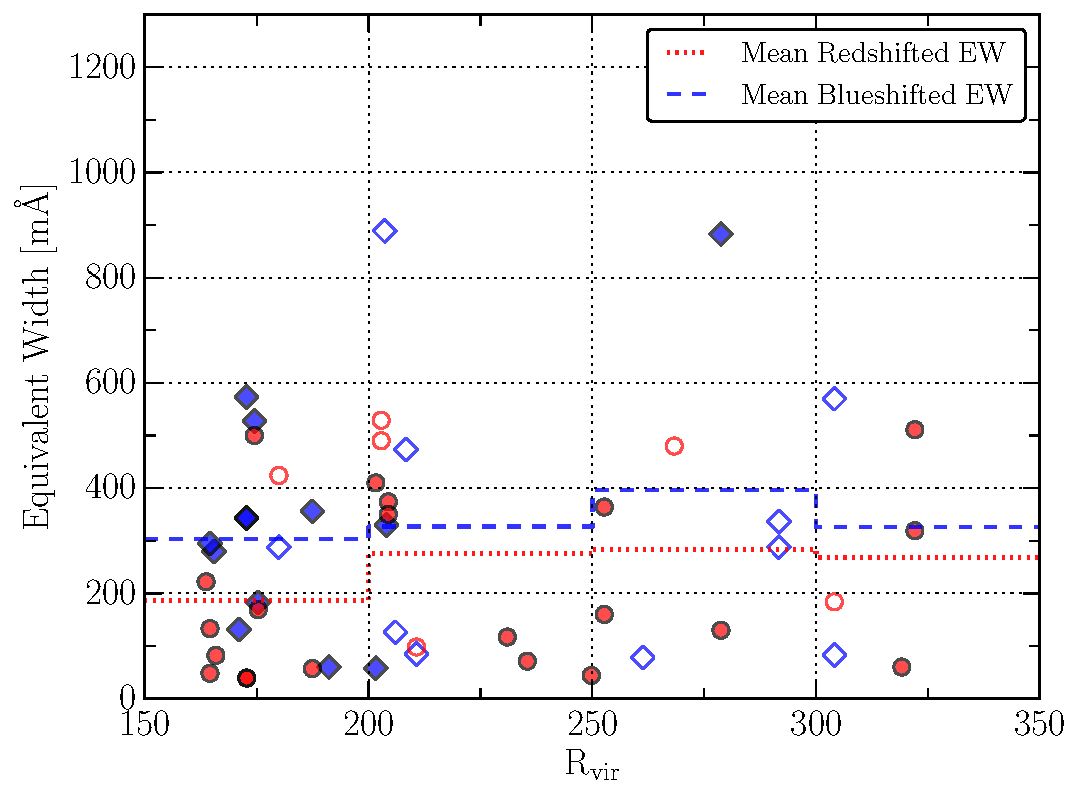
\includegraphics[width=0.49\textwidth]{Chap3/figures/fig6.pdf}}
\subfigure[]{\label{impact_vir}\includegraphics[width=0.49\textwidth]{Chap3/figures/fig7.pdf}}
\caption{\small{(a) Equivalent width of each absorber as a function of the virial radius of the associated galaxy. (b) Impact parameter to each absorber as a function of the virial radius of the associated galaxy. The black dashed line indicates the cutoff at $\rho/R_{\rm vir} =2.14$ imposed by our $\mathcal{L}$ limit.} In each, the blue dashed and red dotted lines show the average $EW$ in 50 kpc bins of impact parameter for the blueshifted and redshifted absorbers, respectively. Open symbols correspond to systems with $\rho \leq R_{\rm vir}$.}
\vspace{5pt}
\end{figure}


\vspace{10pt}


\subsection{EW-$\rho$ Anti-correlation}
\label{ew}

Numerous previous studies have suggested that Ly$\alpha$ equivalent width ($EW$) is anti-correlated with impact parameter ($\rho$) to the nearest galaxy. We find a weak anti-correlation, as shown in Figure \ref{ew_vs_impact}. However, as Churchill et al. (2013a) also found with Mg \,{\sc ii} absorption, we find a stronger anti-correlation when we normalize $\rho$ by $R_{\rm vir}$. Figure \ref{ew_vs_impact_vir} shows this expected anti-correlation when plotting $EW$ versus $\rho/R_{\rm vir}$. A possible explanation for this trend is that larger galaxies host larger, more physically extended CGM halos. We would thus expect the absorber $EW$ to also correlate positively with $R_{\rm vir}$. Figure \ref{w_vir} shows $EW$ as a function of $R_{\rm vir}$, with the blue-dashed and red-dotted lines showing the average $EW$ in bins of 50 kpc of $R_{\rm vir}$, showing little evidence of a correlation. However, by similarly plotting $\rho$ as a function of $R_{\rm vir}$, we instead find some evidence that absorbers around larger galaxies tend to be found at higher impact parameters. While we expect the upper-left quadrant of this figure to be sparsely populated (our likelihood-based method would tend not to choose small galaxies at large impact parameters), it is unclear to us why the lower right quadrant (large galaxies with absorbers at low impact parameter) is also sparsely populated. The full-sized sample at the completion of our study should provide a clearer picture.


\begin{figure}[h!]
        \centering
        \includegraphics[width=0.8\textwidth]{Chap3/figures/fig8.pdf}
        \caption{\small{Equivalent width of each absorber as a function of the inclination angle of the associated galaxy. The black and dashed gray lines show the mean and 90th percentile $EW$ of all absorbers in bins of $15^{\circ}$. Open symbols correspond to systems with $\rho \leq R_{\rm vir}$.}}
        \label{ew_vs_inclination}
        \vspace{2pt}
\end{figure}

\begin{figure}[h!]
        \centering
        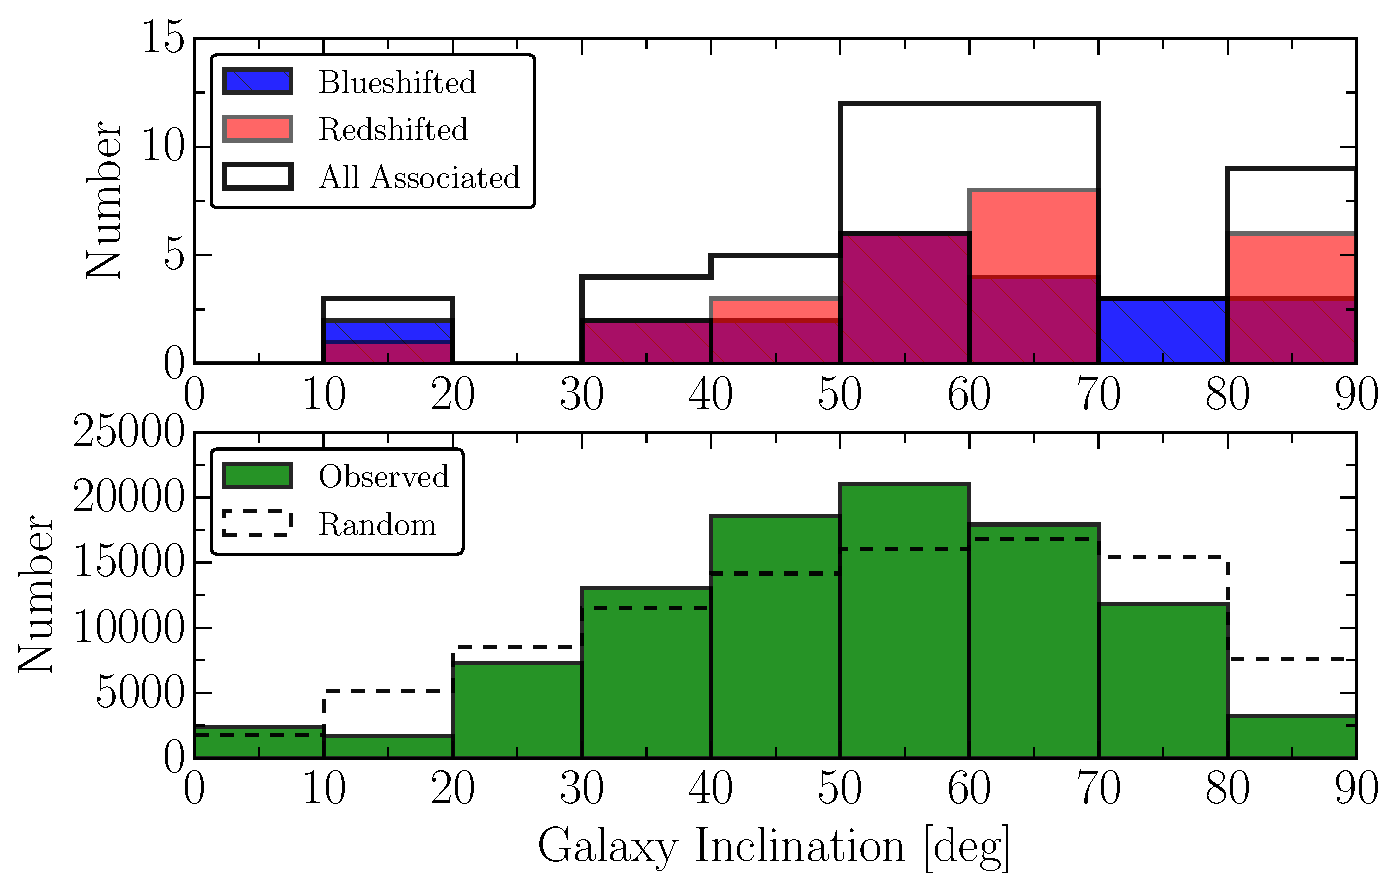
\includegraphics[width=0.8\textwidth]{Chap3/figures/fig9.pdf}
        \caption{\small{Top: distribution of inclinations for all associated galaxies, split into redshifted and blueshifted sets. Bottom: distribution of inclinations of all observed galaxies in the $cz \leq 10,000$ $\rm km\, s^{-1}$ redshift range. The dashed line shows the inclination distribution for a truly random sample (i.e., no observational biases).}}
        \label{hist_inc}
        \vspace{2pt}
\end{figure}


\vspace{10pt}


\subsection{Inclination}
\label{inclination}

In this section we examine the inclinations of the associated galaxies compared to the distributions of absorbers. We correct for the finite thickness of galaxies, which causes $b/a$ to deviate from $\cos(i)$ at high inclinations, by computing galaxy inclinations with the following formula from Heidmann et al. (1972a):

\begin{equation}
	\cos(i) = \sqrt{\frac{q^2 - q_0^2}{1 - q_0^2}},
	\label{incEq}
\end{equation}

\noindent where $q = b/a$, the ratio of the minor to major axis, and $q_0$ is the intrinsic axis ratio, set to $q_0 = 0.2$ for all galaxies (e.g., Jones, Davies, and Trewhella 1996). Of the 48 total absorbers, 6 are associated with E or S0 type galaxies, but we have chosen to keep the value of $q_0 = 0.2$ uniform throughout. The calculated values of $\cos(i)$ that we use for these galaxies are thus conservative underestimates of their true inclinations.

Figure \ref{ew_vs_inclination} shows red and blueshifted absorbers' $EW$ plotted against the inclinations of their associated galaxies. We note that there is a clear excess of absorbers near galaxies of high inclination, with $77\%$ of redshifted and $73\%$ of blueshifted absorbers being associated with galaxies of $i \geq$ 50 deg, and only 3 absorbers being associated with a galaxy of $i<35$. The black and grey-dashed lines show mean and 90th percentile histograms, respectively, in bins of 12 deg. There does not appear to be much evolution of $EW$ across galaxy inclination, although a slight increase of mean $EW$ is possibly present toward higher inclinations.

In total, $75\%$ of absorbers are associated with highly inclined galaxies ($i \geq$ 50 deg). Only $56\%$ of all galaxies in the survey volume are highly inclined, indicating a preference for detecting absorption around inclined galaxies. Figure \ref{hist_inc} shows the distribution of galaxy inclinations for both the red and blue-shifted associated galaxies and all galaxies within the survey volume. We tested the difference between the full distribution of inclination angles for all galaxies in our survey volume and the distribution for all associated galaxies (red + blue-shifted absorbers) using the Anderson-Darling (AD) statistical distribution test, yielding a $p$-value of $AD_{p} = 0.00037$. Thus at a $99.96\%$ confidence level ($\sim 3.6 \sigma$ for a normal distribution) the inclinations of our associated galaxies are not sampled from the average distribution of observed inclinations. Hence, we take this to mean that the shape of the CGM of these galaxies is not perfectly spheroidal. 

It is worth noting here that the observed distribution of galaxy inclinations is \emph{not} flat, as one might naively expect. The dashed line in Figure \ref{hist_inc} shows the distribution of observable inclinations for a random, uniform sample (i.e., a uniform distribution of $q=b/a$ values between 0.2 and 1.0). There could be a number of effects contributing to the difference between this expected distribution and the observed (shown in green). If our sample is magnitude-limited and we assume galaxies are mostly optically thin but with a very-thin optically thick component (e.g., a dust lane), then mostly face-on and mostly edge-on galaxies would be underrepresented due to surface brightness and dust obscuration effects (e.g., see Jones, Davies and Trewhella 1996). It is possible that a similar effect is also responsible for the overabundance of Ly$\alpha$ detections around highly inclined galaxies. If we assume a disky or oblate spheroid halo shape and a covering fraction below unity for the CGM, the probability of encountering a cloud near an inclined galaxy would increase due to the increased path-length through the halo. We will produce a model to test this and other possible explanations in Paper II, when we have the much larger dataset available.

\vspace{10pt}


\subsection{Velocity Difference \rm($\Delta v$\rm)}
\label{veldiff}

\begin{figure}[ht!]
        \centering
        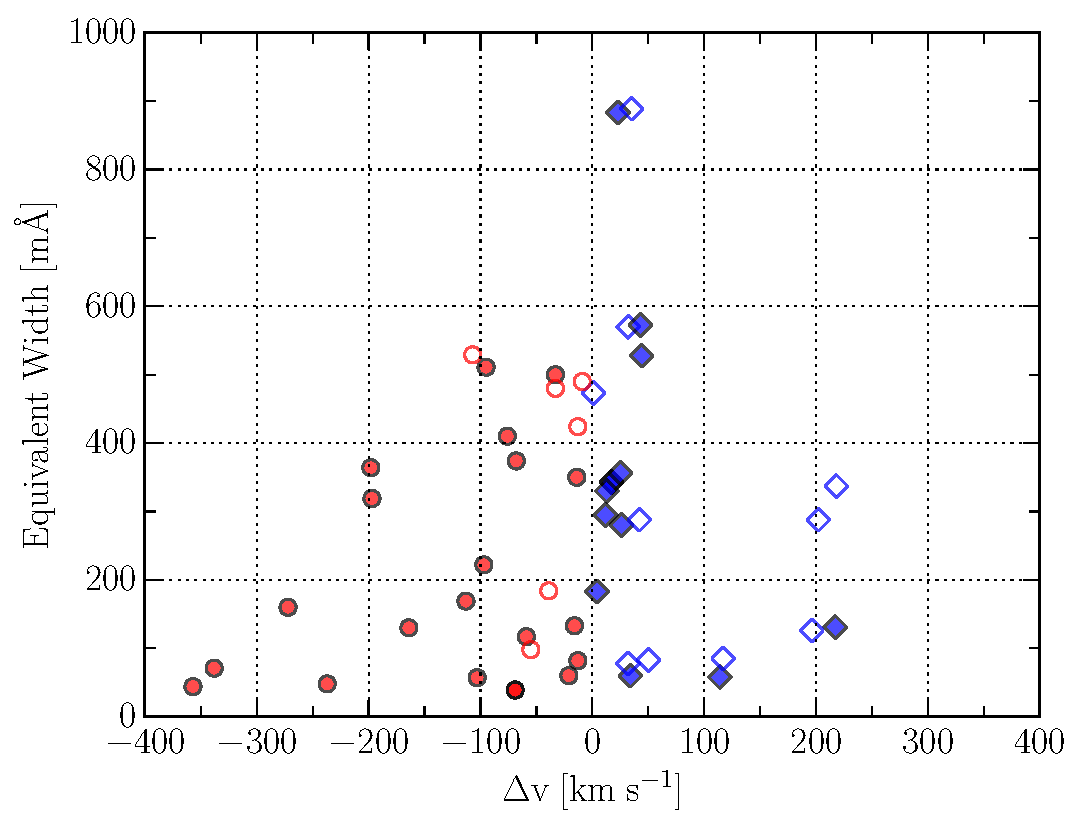
\includegraphics[width=0.8\textwidth]{Chap3/figures/fig10.pdf}
        \caption{\small{Equivalent width as a function of the velocity separation between the galaxy and absorption line. Open symbols correspond to systems with $\rho \leq R_{\rm vir}$.}}
        \label{W_veldif}
        \vspace{5pt}
\end{figure} 

We find evidence for an anti-correlation between absorber $EW$ and the velocity difference between the galaxy and the associated absorption, $\Delta v$. The mean and maximal $EW$ of absorption increases with decreasing $\Delta v$ (see Figure \ref{W_veldif}). In total, 32/48 ($67\%$) of absorbers are found within $\pm100$ $\rm km\, s^{-1}$. This $\pm100$ $\rm km\, s^{-1}$ threshold also applies to absorber $EW$, with only 1 absorber of $EW \geq 400$ found with $\Delta v > 100$ $\rm km\, s^{-1}$. 

Blueshifted absorbers are on average closer both in velocity and impact parameter to their associated galaxy, with $\overline{\Delta v}_{blue} = 68\pm16$ $\rm km\, s^{-1}$ and $\overline{\rho_{blue}} = 218\pm17$ kpc,  compared to $\overline{\Delta v}_{red}=-108\pm20$ $\rm km\, s^{-1}$ and $\overline{\rho_{red}} = 298\pm23$ kpc for the redshifted sample. Correspondingly, blueshifted absorbers have a slightly higher average equivalent width, $\overline{EW}_{blue}=329\pm52$ $\rm m\AA$ compared to $\overline{EW}_{red}=245\pm34$ $\rm m\AA$.

Additionally, of the 48 associated absorbers, 29 are matched with the same galaxy as another absorber (for a total of 14 unique galaxies in this subset). All but one of these cases involve two absorbers in the same sightline yet separated in velocity around a galaxy. Of these, 23 out of 29 are oriented such that the higher $EW$ absorber has the smaller $\Delta v$, and the 6 others are close in either velocity or $EW$. The one galaxy with three associated absorbers, NGC1097, shows this trend across two sightlines as well, with absorbers at $\Delta v = 32$ $\rm km\, s^{-1}$ and $EW = 570$ $\rm m\AA$ toward 2dFGRS\_S393Z082, and $\Delta v = -39$ $\rm km\, s^{-1}$ and $EW = 184$ $\rm m\AA$ and $\Delta v = 50$ $\rm km\, s^{-1}$ and $EW = 83$ $\rm m\AA$ toward HE0241-3043.

This result is the opposite of what we might expect selection effects associated with our likelihood method to produce. Because $\mathcal{L}$ is small for both high $\Delta v$ and high $\rho / R_{\rm vir}$, there should be mostly low $\rho / R_{\rm vir}$ systems at high $\Delta v$. Low $\rho / R_{\rm vir}$ systems should also have higher $EW$ on average, as evidenced in the $EW-\rho$ anti-correlation discussed above. Figure \ref{W_veldif} shows the opposite, however, with only low-$EW$ systems at high $\Delta v$. It must therefore be the case that $EW$ tends to anti-correlate with both $\Delta v$ \textit{and} $\rho / R_{\rm vir}$. Disentangling the relative strengths of the correlations between $EW$ and $\rho$, $R_{\rm vir}$, and $\Delta v$ will require a larger data set, and thus we defer this discussion to our forthcoming Paper II of this series.

\vspace{10pt}

\subsection{Azimuth}
\label{azimuth}


\begin{figure}[t!]
        \centering
        \includegraphics[width=0.7\textwidth]{Chap3/figures/fig11.pdf}
        \caption{\small{Azimuth is the angle, $\alpha$, between the major axis of the galaxy, $a$, and a vector extending from the QSO target to the galaxy center. Image of NGC891 credit: composite Image Data - Subaru Telescope (NAOJ), Hubble Legacy Archive, Michael Joner, David Laney (West Mountain Observatory, BYU); Processing - Robert Gendler.}}
        \label{azimuth_illustration}
        \vspace{5pt}
\end{figure} 

\begin{figure}[t!]
        \centering
        \includegraphics[width=0.8\textwidth]{Chap3/figures/fig12.pdf}
        \caption{\small{The distributions of azimuth angles for red and blue-shifted samples, with the combined sample plotted in black. Azimuth $= 0$ corresponds to absorption detected along the projected major axis of the galaxy, and Azimuth $= 90$ is along the minor axis.}}
        \label{azimuth_dist}
%        \vspace{5pt}
\end{figure}

In this section we examine properties of absorbers as a function of their azimuthal angle with respect to their associated galaxy. Azimuth is defined as the angle between the major axis of a galaxy and the vector connecting the absorption feature and the midpoint of the galaxy plane. Figure \ref{azimuth_illustration} illustrates this. 

The mean azimuth angle for blueshifted absorbers is $43\pm5^{\circ}$, and $49\pm5^{\circ}$ for redshifted absorbers. Figure \ref{azimuth_dist} shows the distribution of azimuth angles for both red and blue-shifted absorbers. Unlike the findings of Kacprzak et al. (2011b, 2012a), who find a bimodal distribution of Mg\,{\sc ii} absorbers around galaxies, our distributions of Ly$\alpha$ absorbers are generally consistent with a flat, or random distribution. There is possibly a slight overabundance of redshifted absorbers around $0^{\circ}$ (minor axis) and blueshifted absorbers between 20 and $50^{\circ}$ (just off major axis), but we cannot assign this observation much significance yet, given the small sample size. We additionally find no significant correlation between azimuth angle and $EW$ or $\Delta v$. See Figure \ref{azimuthMap} for a map of the locations of absorbers relative to their associated galaxies, split between redshifted and blueshifted absorbers and into three bins of inclination.

\begin{figure}[ht!]
        \centering
        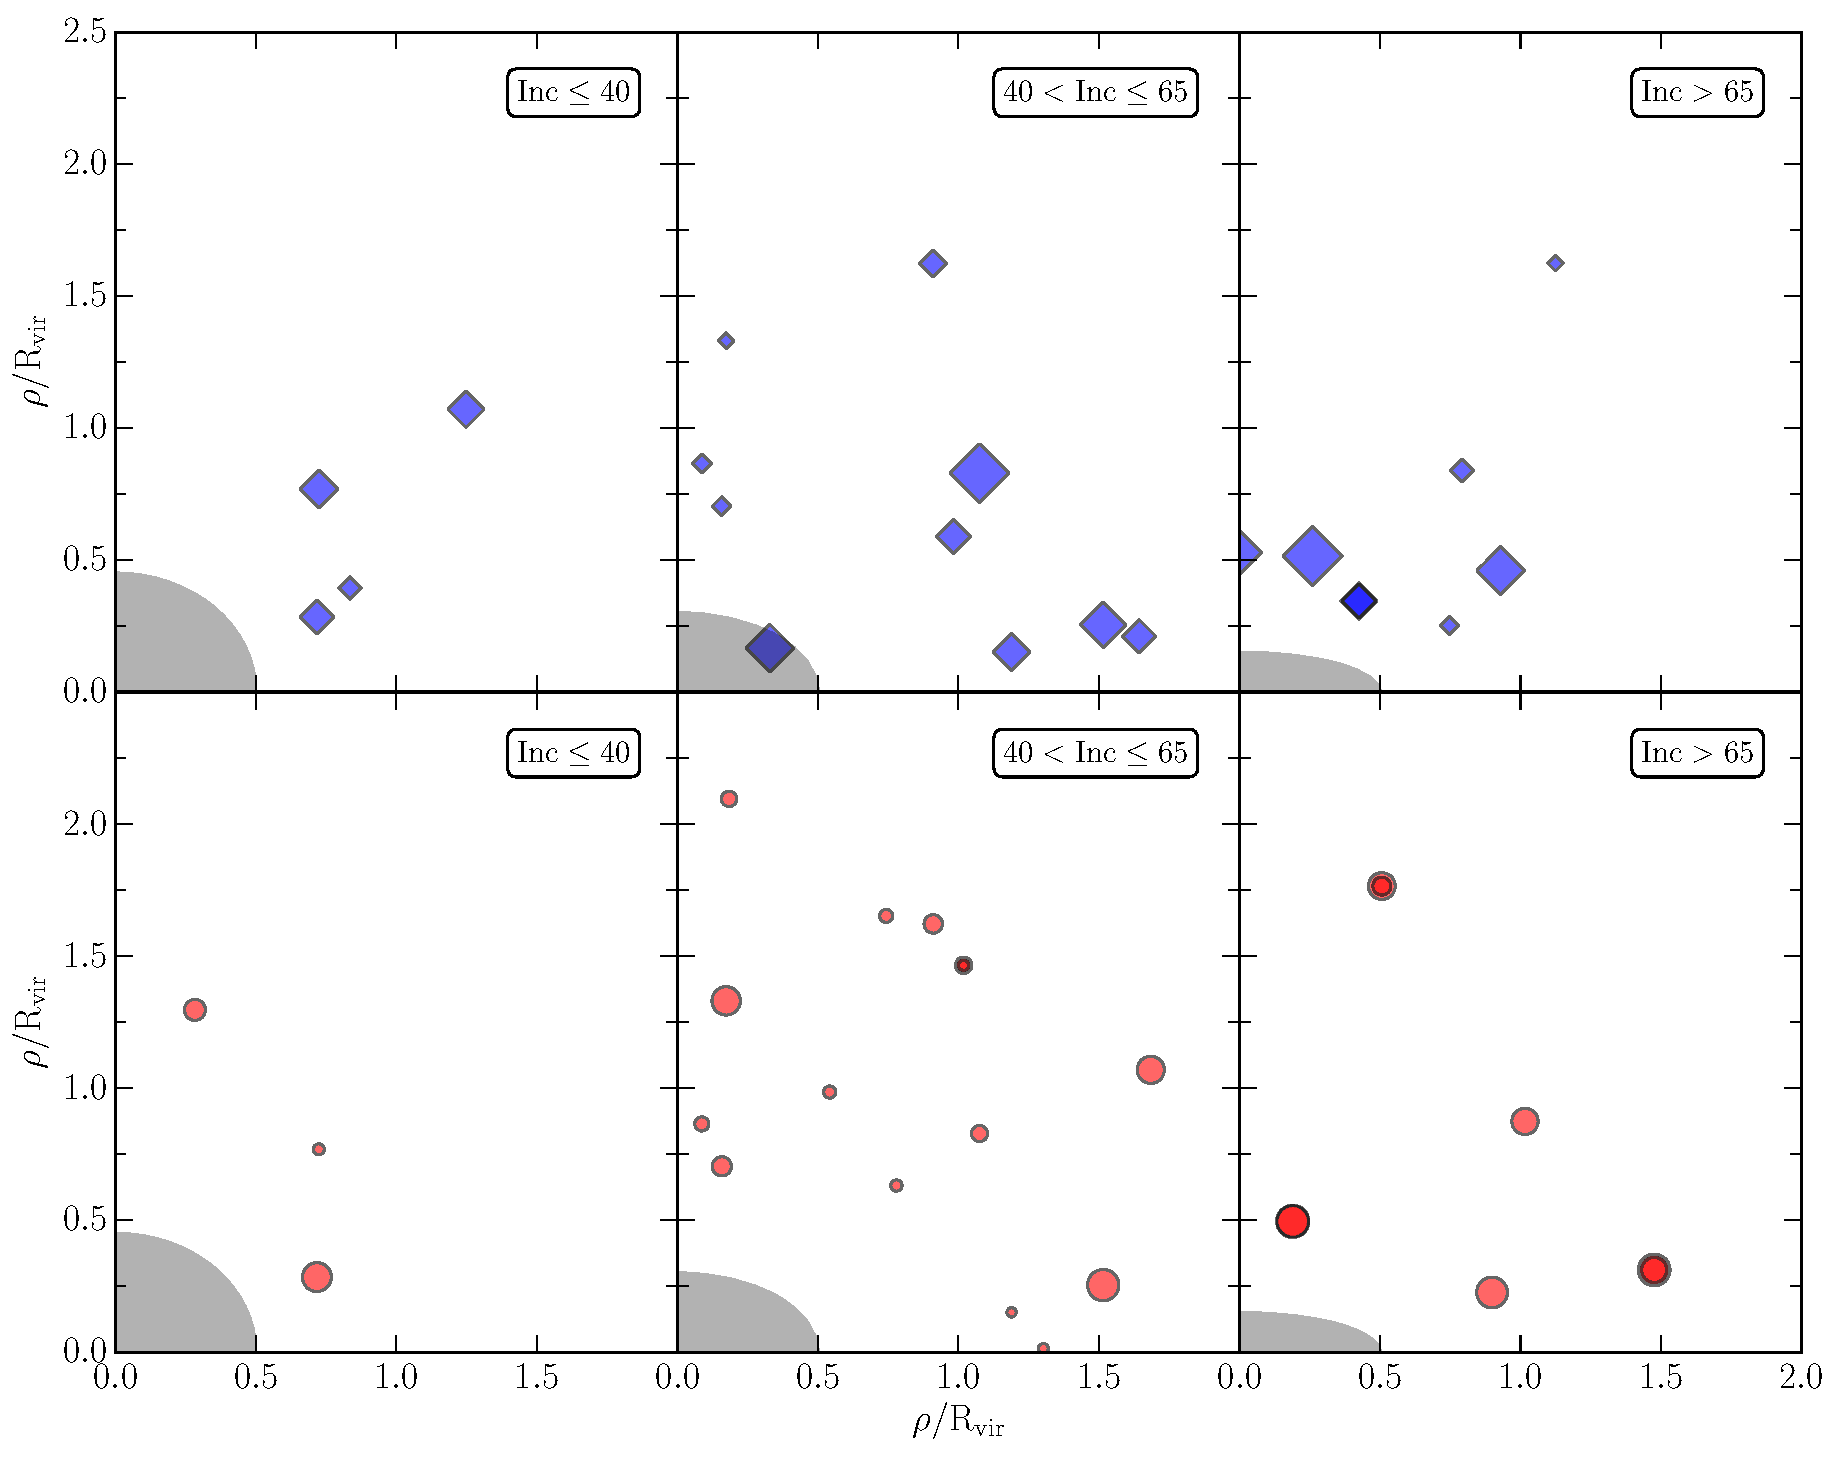
\includegraphics[width=0.99\textwidth]{Chap3/figures/fig13.pdf}
        \caption{\small{A map of where each absorber was detected with respect to the associated galaxies, separated into three bins of inclination (illustrated by the gray ellipse in the bottom left corner of each plot). Left: absorbers associated with galaxies of inclination $0 \leq Inc \le 40$; center: $40 \leq Inc \le 65$; and right: $65 \leq Inc$. Blueshifted and redshifted absorbers are separated into the top (diamonds) and bottom (circles) panels, and the marker size is scaled with $EW$. The sightlines containing multiple absorbers associated with the same galaxy can be identified by their darker colors. Open symbols correspond to systems with $\rho \leq R_{\rm vir}$.}}
        \label{azimuthMap}
%        \vspace{5pt}
\end{figure} 

These contrasting results may indicate a genuine difference between the properties of Ly$\alpha$ and metal lines, since the distributions of the latter are thought to be influenced by outflows, which may be focused along the minor axis.


\section{Discussion}


In this paper we have chosen to separate absorption systems into their individual components, whereas many comparable CGM studies have instead chosen to group together absorption components within some velocity window. While making the assumption that absorbers within some velocity interval are physically linked certainly has merit, it is also possible that absorption components close in velocity may in fact be physically distinct (see, e.g., Churchill et al. 2015). Indeed, in Section \ref{veldiff} we identified several systems where the $EW$ of components of a possible Ly$\alpha$ system individually anti-correlated with $\Delta v$. We will thus explore both methods in Paper II, where the much larger sample size will allow for a meaningful comparison.\\

Restricting ourselves to low-redshift systems has several benefits and consequences. We are able to extend our search for associated galaxies to larger impact parameters than many related, higher-redshift CGM studies, because of the availability of galaxy data. However, due to the observed anti-correlation between $EW$ and impact parameter, this results in a larger fraction of low-$EW$ and low-column density absorbers in our sample. Hence, we are likely tracing a region of the CGM not entirely analogous to that traced by, e.g., Kacprzak et al. (2011b), Mathes et al. (2014), and Borthakur et al. (2015).

Studies focusing on metal lines (e.g., Mg\,{\sc ii} and O\,{\sc vi}) are generally associated with high column density Lyman Limit Systems (LLS), which, again, tend to originate closer to their host galaxies. Most of the Ly$\alpha$ absorbers in this work are low column density (generally log$~N$(H\,{\sc i}) $\leq$ 14), and originate near or beyond 1 $R_{\rm vir}$. At these distances we may actually be probing the interface between CGM associated with individual galaxies and the larger-scale network of intergalactic gas filaments, thus the lack of any correlation with azimuth angle is not wholly unexpected.

We do, however, detect an inclination effect on the density, and possibly $EW$, of Ly$\alpha$ absorbers. The combination of no azimuthal dependence and increased absorber density with inclination leads us to conclude that these galaxies have disk-like, oblate-spheroidal halos. A perfectly spheroidal halo would show no correlation for either, and an extremely flattened halo would show up as enhanced number density along the major axis. These results are consistent with a picture where the H\,{\sc i} covering fraction steadily decreases from $\sim$unity very near to galaxy disks out to at least 1 Mpc, where gas associated with galaxies merges with the general IGM. Our larger upcoming dataset will provide the statistics necessary to probe this in finer detail, as well as give clues regarding the exact shape of this fall-off and the level of clumpiness or filamentary structure in galaxies' H\,{\sc i} halos.

\begin{deluxetable}{l c c }
\tablewidth{0pt}
\tabletypesize{\footnotesize}
\tablecaption{Average properties of the associated galaxy sample split into red and blue-shifted bins based on $\Delta v$\label{resultsTable}}
\tablehead{
\colhead{Statistic} \hspace{1.6cm} 		&  \colhead{\hspace{1.6cm} Blueshifted Absorbers} \hspace{1.6cm} 	&  \colhead{ \hspace{.7cm}Redshifted Absorbers} \hspace{.7cm}}
\startdata
 Number 	          			 		&     	22				&	26			\\
 Mean $EW$    \scriptsize $\rm [m\AA]$    &	$329 \pm 52$ 		&	$245 \pm 34$  	\\
 Median EW     \scriptsize $\rm [m\AA]$    & 	$292 \pm 16$		& 	$177 \pm 10$	\\
 Mean $\rm R_{\rm vir}$   \scriptsize [kpc]	&   	$215 \pm 10$		& 	$224 \pm 10$	\\
 Mean $\rho$   \scriptsize [kpc]          		&   	$218 \pm 17$ 		& 	$298 \pm 23$	\\
 Mean $\Delta v$  \scriptsize $\rm [km\, s^{-1}]$     &	$ 68 \pm 16$    &	$-108 \pm 20$	\\
 Mean Inc.  \scriptsize [deg]  			&  	$58 \pm 4$		&	$61 \pm 4$	\\
 Mean Az.  \scriptsize [deg]    			&	$43 \pm 5$ 		&	$49 \pm 5$ 	\\
\enddata 
\tablecomments{All reported errors are standard errors in the mean.}
%\vspace{-5pt}
\end{deluxetable}



%\begin{table}[b]\footnotesize
%  \caption{\small{Average properties of the associated galaxy sample split into red and blue-shifted bins based on $\Delta v$}}
%  \vspace{-20pt}
%\begin{center}
%\begin{tabular}{l l l}
% \hline \hline
% Statistic                				&  Blueshifted Absorbers   &     Redshifted Absorbers     \\ 
%  \hline \hline
% Number 	          			 		&     	22				&	26			\\
% Mean $EW$    \scriptsize $\rm [m\AA]$    &	$329 \pm 52$ 		&	$245 \pm 34$  	\\
% Median EW     \scriptsize $\rm [m\AA]$    & 	$292 \pm 16$		& 	$177 \pm 10$	\\
% Mean $\rm R_{\rm vir}$   \scriptsize [kpc]	&   	$215 \pm 10$		& 	$224 \pm 10$	\\
% Mean $\rho$   \scriptsize [kpc]          		&   	$218 \pm 17$ 		& 	$298 \pm 23$	\\
% Mean $\Delta v$  \scriptsize $\rm [km\, s^{-1}]$     &	$ 68 \pm 16$    &	$-108 \pm 20$	\\
% Mean Inc.  \scriptsize [deg]  			&  	$58 \pm 4$		&	$61 \pm 4$	\\
% Mean Az.  \scriptsize [deg]    			&	$43 \pm 5$ 		&	$49 \pm 5$ 	\\
% 
%\hline
%\end{tabular}
%
%\footnotesize \raggedright \textbf{Note.} All reported errors are standard errors in the mean.
%\end{center}
%\label{resultsTable}
%\end{table}

\vspace{5pt}

\section{Summary}

We have introduced a novel likelihood method for associating absorption systems with nearby galaxies, and explored its implementation with a small subsample of 33 COS sightlines. Associating CGM absorbers with individual galaxies remains a difficult and ambiguous affair, but with this new metric we can at least do so in a reproducible and numerical manner. 

In this pilot sample we have measured 48 $\rm Ly\alpha$ absorption lines in the spectra of 33 COS targets and matched each to a single, large ($D\geq 25$ kpc) galaxy. Table \ref{resultsTable} presents a breakdown of our results when separating absorber-galaxy pairs into red and blue-shifted samples. The following summarizes our findings:

\vspace{10pt}

\begin{enumerate}

\item We introduce a likelihood parameter, $\mathcal{L}$, based on Gaussian profiles centered around $\rho / R_{eff}$ and $\Delta v / v_{\rm norm}$ to automate the matching of absorbers with associated galaxies. The response of $\mathcal{L}$ can be tailored by choosing different values for $R_{eff}$ and $v_{\rm norm}$ (we used $R_{eff}$ = [$R_{\rm vir}$, $D^{1.5}$] and $v_{\rm norm}$ = 200 $\rm km\, s^{-1}$ in this work, and will explore other parameterizations in a future paper).

\item Equivalent width ($EW$) anti-correlates most strongly with $\rho$ when normalized by $R_{\rm vir}$. It follows that $EW$ weakly correlates and anti-correlates with $R_{\rm vir}$ and $\rho$, respectively.

\item The mean and maximal $EW$ of absorbers increase with decreasing $\Delta v$. The strongest absorbers are nearly all found within $\Delta v = \pm 100$ $\rm km\, s^{-1}$ of their associated galaxies.

\item $\rm Ly\alpha$ absorbers are most commonly associated with inclined galaxies. $73\%$ of blueshifted and $77\%$ of redshifted absorbers are associated with galaxies with $i \geq 50$ deg, whereas $56\%$ of all galaxies in the survey volume have similarly high inclinations. The distributions of associated versus all galaxy inclinations differ at a greater than $99\%$ confidence, or $\sim 3.6\sigma$ level, according to the Anderson-Darling distribution test.

\item We find no strong evidence for azimuth preference for absorption - Ly$\alpha$ absorbers appear to be distributed uniformly around galaxy major and minor axes.

\end{enumerate}

In a future paper we will apply this method to a sample of hundreds of COS sightlines in an effort to produce the most statistically robust CGM study to date.


\acknowledgements

We would like to thank the referee for his/her valuable comments and suggestions. This research has made use of the NASA/IPAC Extragalactic Database (NED) which is operated by the Jet Propulsion Laboratory, California Institute of Technology, under contract with the National Aeronautics and Space Administration. This work is based on observations with the NASA/ESA \textit{Hubble Space Telescope}, obtained at the Space Telescope Science Institute (STScI), which is operated by the Association of Universities for Research in Astronomy, Inc., under NASA contract NAS 5-26555. Spectra were retrieved from the Barbara A. Mikulski Archive for Space Telescopes (MAST) at STScI. Over the course of this study, D.M.F. and B.P.W. were supported by grant AST-1108913, awarded by the US National Science Foundation, and by NASA grants \textit{HST}-AR-12842.01-A, \textit{HST}-AR-13893.01-A, and \textit{HST}-GO-14240 (STScI).
%
%\facility{HST (COS)}


\nocite{*}
\bibliographystyle{thesis}
%\bibliography{/Users/clairemurray/Desktop/DMF_thesis/Chap3/chap3}
\bibliography{/Users/frenchd/Research/inclination/git_inclination/thesis/DMF_thesis/Chap3/chap3}




\chapter[Evidence for a Rotational Component in the CGM of Nearby Galaxies]{Evidence for a Rotational Component in the CGM of Nearby Galaxies}
\label{chap:chap4}

% Leave space between title and quote or publication note.  This has often been
% 10cm for a quote and 8 cm for a reference, but this is really up to you.
%\vspace{8cm}

\vfill

\begin{flushright}
  \fixspacing % Single spacing
  \textit{To be submitted to the \emph{Astrophysical Journal}} \\
%  \vspace{1ex} Tofflemire, et al.\ 2017, \apj, 835, 8
\end{flushright}

\vspace*{1in} % Leave a 1-in space at the bottom.

\cleardoublepage

\begin{chabstract}

We present results of a study comparing the velocity of $\rm Ly\alpha$ absorbers relative to the rotation direction and velocity of nearby galaxy disks in the nearby Universe ($z \leq 0.03$). We have obtained rotation curves via long-slit spectroscopy of 12 galaxies with the Southern African Large Telescope, and combine this dataset with an additional 17 galaxies with published rotation curves from the literature. Each galaxy appears within $3 R_{\rm vir}$ of a QSO with available Cosmic Origin Spectrograph (COS) data covering the relevant $\rm Ly\alpha$ wavelength range. We present a simple cylindrical galaxy halo rotation model to interpret these data in the context of probing three-dimensional galaxy halos via 1-dimensional QSO absorption-line spectroscopy. Relative to this model we find that up to $63\%$ of $\rm Ly\alpha$ absorbers are consistent with co-rotation. Intriguingly, the $\rm Ly\alpha$ co-rotation fraction decreases with both virial radius, scaled impact parameter ($\rho / R_{\rm vir}$), and galaxy luminosity (\Lstar) in a model independent fashion. Finally, we report that both anti-rotating absorbers and those found near luminous galaxies ($L \gtrsim 0.6$\Lstar) mostly have low Doppler b-parameters ($b \lesssim 50$ \kms). Co-rotating absorbers show a wide range of b-parameters. These results are broadly in agreement with the co-rotation fractions predicted by the \cite{stewart2011b} simulations, and furthermore provides some of the first observational evidence for cold-mode accretion onto sub-\Lstar~ galaxies in the low-$z$ Universe. 

%We discuss the implications of these results with respect to the theoretical predictions of cold versus hot mode accretion in the low-$z$ Universe.

\end{chabstract}


%\keywords{galaxies:intergalactic medium, galaxies:evolution, galaxies:halos, quasars: absorption lines}


\section{Introduction}
Our current Lambda Cold-Dark-Matter ($\Lambda$CDM) cosmology picture describes galaxies forming hierarchically out of overdensities in the underlying dark matter distribution. As the surrounding intergalactic medium (IGM) is funneled toward a growing galaxy, simulations predict the angular momentum of the inflowing gas is redistributed onto the disk and seeds the overall rotation of the galaxy (e.g., \citealt{stewart2011a, chen2003, sharma2005, brook2011, kimm2011, pichon2011, stewart2013}). As this infalling gas is responsible for birthing and continuing to feed the galaxies throughout their lifetimes, it is expected that the extended gaseous halos should rotate in the same sense as both the galactic disks and dark matter halos. 

In the $\Lambda$CDM picture, accretion falls broadly into two types. In the so-called ``hot-mode", gas shock-heats at the virial radius as it encounters the galaxy halo. The inner, more dense region of this hot gaseous halo then rains down onto the disk as it radiatively cools (e.g., \citealt{fillmore1984, bertschinger1985, danovich2012, shen2013}). However, most gas arrives cold ($T\sim 10^{4}$ K) from the IGM, and the proposed radiative shock is unstable to cooling. Thus this hot-halo scenario may not actually be created \citep{birnboim2003, keres2005, ocvirk2008, brooks2009, dekel2009}.


% From vandevoort2011 - Hence, hot accretion will dominate for the most massive haloes. The dominant form of accretion will thus depend on both the mass of the halo and accretion redshift 
%(Birnboim & Dekel 2003; Katz et al. 2003; Kere� et al. 2005; Ocvirk, Pichon & Teyssier 2008; Brooks et al. 2009; Kere� et al. 2009a; Crain et al. 2010)


%all this from Pichon 2011 (MNRAS 418, 2493?2507) See also Binney 1977. 

In contrast, as part of  the alternative ``cold-mode" accretion model, filaments of gas from the IGM should merge smoothly with the disk, thus converting a significant fraction of their infall velocity to rotational velocity of the galaxy \citep{keres2005,stewart2017}. The simulations of \cite{powell2011} agreed with these conjectures by showing that indeed, the accreting filaments connect rather smoothly to the disc, even in the presence of strong supernova driven winds. This cold-mode of accretion likely dominates the global growth of all but the most massive halos at high redshifts ($z \gtrsim 3$), and the growth of lower mass ($M_{\rm halo} \leq 5 \times 10^{11} ~M_{\rm *}$) objects at late times \citep{dekel2006, vandevoort2011}. Furthermore, cosmological SPH simulations such as those by \cite{stewart2011b, stewart2013} suggests that halo gas should co-rotate with disk-gas out to at least 100 kpc, and that absorption in intervening QSO sightlines should be able to accurately capture this rotation signature. 

%Galaxy rotation curves have been observed to extend at constant velocity out to... (cite...). It becomes increasingly difficult to measure gas rotation much farther from this however as the density rapidly decreases. Within this region the galaxy disks transition into circumgalactic medium (CGM), and eventually the CGM merges with the intergalactic medium (IGM). At what point, however, does the surrounding medium cease to circulate with the galaxy? A standard tool for probing gas at large radii from galaxies is QSO absorption line spectroscopy. 

 

Some observational evidence of cold-mode accretion has been obtained at higher redshifts. In pioneering studies focusing on the Mg\II~absorber kinematics and their connection with neighboring galaxies, \cite{charlton1998, steidel2002}, and later \cite{kacprzak2010, ho2017}, find tantalizing evidence that a significant fraction of Mg\II~absorbers have velocities that can be explained by an extended gaseous disk. Additionally, \cite{diamond-stanic2016} detect co-rotating H$\alpha$ emission and Mg\,{\sc ii} and Fe\,{\sc ii} absorption toward a Milky Way-like galaxy at $z=0.413$. However, as noted by \cite{steidel2002}, a simple extended disk model is insufficient to explain the observed bulk motion implied by their sample of 5 Mg\II~absorber-galaxy systems, and a rotating \emph{halo} may be a better model.

%However, as noted by Steidel 2002, a rotating \emph{halo} may be a better model than a simple extended thick disk model based on . 

Additionally, the picture may have changed since $z \sim 0.5$, the epoch 5 Gyr ago that most of these Mg\II~systems are probing. By $z \sim 0$ simulations (e.g., \citealt{keres2005, stewart2017}) predict a drop-off in cold-mode accretion and a decrease in the density of IGM filaments. Observational confirmation has been even more inconclusive in this low-redshift regime. In the largest such study, involving Ly$\rm \alpha$ absorber-galaxy kinematics, \cite{cote2005} probed the halos of nine galaxies using \emph{HST} observed background QSOs, and found that large warps would be needed to explain the velocity of \HI~absorbers by an extended rotating disk. \cite{wakker2009} compiled a sample of 76 sightlines, which included only 4 galaxy-QSO systems for which the galaxy's rotation curve was known from the literature, and finding only 1/4 of Ly$\alpha$ absorbers appeared to co-rotate with the associated galaxy disk. Similarly, \cite{kacprzak2011_kinematics} claim a reduction in Mg\II~co-rotation around $\rm \sim $\Lstar~ galaxies between $z\sim 0.5$ and $z\sim 0.1$. Approaching the question from a different angle, \cite{bowen2016} probed the halo of a single galaxy, NGC1097, with 4 nearby QSO sightlines, and suggests that an extended, slowly rotating disk with additional inflowing IGM material best matches observations. 

%The largest study of low-redshift, Ly$\rm \alpha$ absorber-galaxy kinematics was \cite{cote2005}, which worked with a  sample of 5 galaxy-absorber systems. 

%This cold-mode accretion should dominate the global growth of all galaxies at high redshifts (z ? 3) and the growth of low-mass (Mhalo ? 5 � 1011 M) objects at late times (Dekel & Birnboim 2006).

%his infalling gas is shock-heated and slowly cools (\cite{danovich2012}, \cite{shen2013}). As this infalling gas is responsible for birthing and continuing to feed the galaxies, it is expected that the extended gaseous halos should rotate in the same sense as both the galactic disks and dark matter halos. 

%As matter is funneled toward a growing galaxy, simulations predict conservation of angular momentum redistributes the angular momentum in this gas to match that of the halo and underlying dark matter as the gas is shock-heated and slowly cools (\cite{danovich2012}, \cite{shen2013}). As this infalling gas is responsible for birthing and continuing to feed the galaxies, it is expected that the extended gaseous halos should rotate in the same sense as both the galactic disks and dark matter halos. 

%There have been several studies with a sample size of one or a few aiming to compare the kinematics of the galaxy disk to absorption detected in it's CGM halo (e.g., C\^{o}t\'{e} et al. 2005; Wakker \& Savage 2009; Bowen et al. 2016; \textbf{MORE}). With these individual results we may be missing the forest for the sake of the individual trees. There has yet to be a more systematic search for observational evidence that the CGM is kinematically associated with galaxies in general.


%Numerous studies have shown a correlation between equivalent width and decreasing velocity difference between galaxies and IGM absorbers (e.g., \citealt{french2017}, MORE).

To significantly improve observational statistics in this low-redshift regime, we have obtained rotation curves from the Souther African Large Telescope (SALT) for 12 nearby spiral galaxies which are located within $3 R_{\rm vir}$ kpc of a background QSO observed by the Cosmic Origins Spectrograph (COS) on \textit{HST}. A literature search yielded an additional 17 galaxies with published rotation curves and known orientations. Each of these is probed by at least one QSO within $3 R_{\rm vir}$.

In Section \ref{data} we describe the selection and reduction of both SALT and COS spectra. In Section \ref{model} we present a new rotating halo model we have developed to aid in the interpretation of our observations. In Section \ref{discussion} we discuss the overall results of this exercise and present a physically-motivated interpretation of these results. See Section \ref{summary} for a summary of our results and conclusions. Each galaxy-QSO system is discussed in detail in Appendix \ref{SALT_sample}.



\begin{deluxetable}{l l l l l l l l l l}
\rotate
\tablewidth{0pt}
\tabletypesize{\footnotesize}
\tablecaption{SALT Galaxy Observations\label{tab:params}}
\tablehead{
\colhead{Galaxy}	&  \colhead{R.A.}	&  \colhead{Dec.}  	&  \colhead{Measured $v_{\rm sys}$}& \colhead{Published $v_{\rm sys}$} & \colhead{Type}	&  \colhead{$v_{\rm rot}$}	& \colhead{$v_{\rm rot} / \sin(\emph{i})$}	& \colhead{Obs. Date} & \colhead{$T_{\rm exp}$}  \\
			  	&          			&  			 	& \colhead{(\kms)}  				& \colhead{(\kms)}  		     	   &					&  \colhead{(\kms)}  		& \colhead{(\kms)}					&					& \colhead{(ks)} \\
\colhead{(1)}  	  	& \colhead{(2)}    	&  \colhead{(3)}   	& \colhead{(4)}  				& \colhead{(5)}    		     	   &	\colhead{(6)}  		& \colhead{(7)}    		&\colhead{(8)}  						& \colhead{(9)}  		& \colhead{(10)}   }
\startdata
 CGCG039-137 	& 11 21 27.0		& +03 26 41.7		& $6918 \pm24$\				&	$6902 \pm 52^{a}$	& Scd			& $132 \pm 16$	& $139 \pm 26$			& 05 11 2016		& 700	\\ %done
 ESO343-G014	 	& 21 37 45.2		& $-$38 29 33.2	& $9139 \pm32$				&	$9162 \pm 45^{b}$	& S				& $203 \pm 32$	& $203 \pm 32$			& 05 16 2016		& 1000	\\ %done
 IC5325		 	& 23 28 43.4		& $-$41 20 00.5	& $1512 \pm8$					&	$1503 \pm 7^{c}$	& SAB(rs)bc		& $53 \pm 5$		& $125 \pm 39$			& 05 17 2016		& 600	\\ %done
 MCG-03-58-009	& 22 53 40.9		& $-$17 28 44.0	& $9015 \pm19$				&	$9030 \pm 10^{d}$	& Sc				& $150 \pm 12$	& $171 \pm 23$			& 05 16 2016		& 1200	\\ %done
 NGC1566		& 04 20 00.4		& $-$54 56 16.1	& $1502 \pm15$				&	$1504 \pm 2^{e}$	& SAB(rs)bc		& $64 \pm 8$		& $195 \pm 47$			& 10 18 2016		& 400	\\ %done
 NGC3513		& 11 03 46.1		& $-$23 14 43.8	& $1204 \pm12$				&	$1194 \pm 7^{c}$	& SB(s)c			& $11 \pm 10$		& $22 \pm 24$				& 05 26 2016		& 600	\\ %done
 NGC3633	 	& 11 20 26.2		& +03 35 08.2		& $2587 \pm7$					&	$2600 \pm 2^{f}$	& SAa			& $149 \pm 6$		& $157 \pm 9$				& 05 11 2016		& 1200	\\ %done
 NGC4536	 	& 12 34 27.1		& +02 11 17.3		& $1867 \pm33$				&	$1808 \pm 1^{g}$	& SAB(rc)bc		& $129 \pm 9$		& $148 \pm 41$			& 05 11 2016		& 1300	\\ %done
 NGC4939		& 13 04 14.4		& $-$10 20 22.6	& $3093 \pm33$				&	$3110 \pm 4^{e}$	& SA(s)bc			& $204 \pm 25$	& $275 \pm 66$			& 05 14 2016		& 500	\\ %done
 NGC5364	 	& 13 56 12.0		& +05 00 52.1		& $1238 \pm17$				&	$1241 \pm 4^{c}$	& SA(rs)bc pec		& $130 \pm 13$	& $155 \pm 22$			& 05 11 2016		& 700	\\ %done
 NGC5786	 	& 14 58 56.3		& $-$42 00 48.1	& $2975 \pm22$				&	$2998 \pm 5^{h}$	& SAB(s)bc		& $156 \pm 10$	& $172 \pm 25$			& 05 11 2016		& 250	\\ %done
 UGC09760	 	& 15 12 02.4		& +01 41 55.5		& $2094 \pm16$				&	$2023 \pm 2^{i}$	& Sd				& $46 \pm 10$		& $46 \pm 16$				& 05 11 2016		& 500	\\
 \hline
\enddata

\tablecomments{SALT targeted galaxies. Columns are as follows: 1) the galaxy name, 2), 3) R.A., Dec. in J2000, 4) measured galaxy systemic velocity, 5) published galaxy systemic velocity, 6) morphological type (RC3), 7) approaching side velocity, 8) receding side velocity, 9) observation date, and 10) exposure time. All observations used the RSS PG2300 grating.}
%\tablenotetext{a}{\cite{sdssDR3}} 
%\tablenotetext{b}{\cite{6dFDR3}}
%\tablenotetext{c}{\cite{RC3}}
%\tablenotetext{d}{\cite{mathewson1996}}
%\tablenotetext{e}{\cite{koribalski2004}}
%\tablenotetext{f}{\cite{RC3}}
%\tablenotetext{g}{\cite{lu1993}}
%\tablenotetext{h}{\cite{grogin1998}}
%\tablenotetext{i}{\cite{koribalski2004}}
%\tablenotetext{j}{\cite{RC3}}
%\tablenotetext{k}{\cite{dinella1996}}
%\tablenotetext{l}{\cite{giovanelli1997}}
%\tablerefs{\cite{giovanelli1997}}
\tablerefs{a. \cite{sdssDR3}; b. \cite{6dFDR3}; c. \cite{RC3}; d. \cite{mathewson1996}; e. \cite{koribalski2004}; f. \cite{lu1993}; g. \cite{grogin1998}; h. \cite{dinella1996}; i, \cite{giovanelli1997}}
 \label{salt_targets}
\end{deluxetable}



%\begin{deluxetable}
%\rotate
%\tablewidth{0pt}
%\tabletypesize{\footnotesize}
%\setlength{\tabcolsep}{0.15in}
%\tablecolumns{7}
%%\tablewidth{2.0pt}
%\tablecaption{Summary of QSO Sample\label{tab:params}}
%\tablehead{
%\colhead{Target}  		&  \colhead{Galaxy} 			&  \colhead{R.A.}  		&  \colhead{Dec.}		& \colhead{z} 	&  \colhead{Program} &  \colhead{${T_{\rm exp}}$}	\\
%			  		&          					&  			 		& 		  			& 		     	&				  & \colhead{(ks)}}
%%\colnumbers
%\startdata
%1H0419-577  				&      NGC1566  		&      04 26 00.7  		&	$-$57 12 02.0  		&   0.10400  	& 11686		& 20429	\\
%2E1530+1511				&	NGC5951			&	15 33 14.3		&	+15 01 03.0		&   0.09000	& 14071		& 9348	\\
%3C232					&	NGC3067			&	09 58 20.9		&	+32 24 02.0		&   0.53060	& 8596		& 44662	\\
%3C273.0  					&	NGC4536  		&      12 29 06.7  		&	+02 03 09.0 		&   0.15834  	& 12038		& 4002	\\
%CSO295					&	NGC3432			&	10 52 05.6		&	+36 40 40.0		&   0.60900	& 14772		& 1088	\\
%CSO1208					&	NGC3726			&	11 40 47.9			&	+46 22 05.0		&   0.11500	& 14729		& 3052	\\
%FBQSJ0908+3246			&	NGC2770			&	09 08 38.8		&	+and/32 46 20.0		&   0.25989	& 14240		& 7430	\\
%H1101-232  				&      NGC3513  		&      11 03 37.7  		&	$-$23 29 31.0  		&   0.18600  	& 12025		& 13341	\\
%HE0429-5343  				&      NGC1566  		&      04 30 40.0  		&	$-$53 36 56.0 		&   0.04001  	& 12275		& 2067	\\
%%HE0435-5304  			&      NGC1566  		&      04 36 50.9  		&      -52 58 47.0  		&   0.42616  	& 11520		& 8372	\\
%%HE0439-5254  			&      NGC1566  		&      04 40 12.0  		&	-52 48 18.0  		&   1.05300  	& 11520		& 8402	\\
%HE1228+0131  				&      NGC4536  		&      12 30 50.0  		&	+01 15 23.0  		&   0.11700  	& 11686		& 11036	\\
%MRC2251-178  			&      MCG-03-58-009  	& 	22 54 05.9  		&	$-$17 34 55.0  		&   0.06609  	& 12029		& 5515	\\
%MRK335					&	NGC7817			&	00 06 19.5		&	+20 12 11.0		&   0.02578	& 11524		&  5122	\\
%MRK771					&	NGC4529			&	12 32 03.6		&	+20 09 30.0		&   0.06301	& 12569		& 1868	\\
%MRK876					&	NGC6140			&	16 13 57.2		&	+65 43 11.0		&   0.12900	& 11524		& 12579	\\
%%MS1047.3+3518			&	NGC3432			&	10 50 10.9		&	+35 02 02.0		&   0.04125	& 8316		&  8301	\\
%PG0804+761				&	UGC04238		&	08 10 58.7		&	+76 02 43.0		&   0.10200	& 11686		& 5510	\\
%PG1259+593				&	UGC08146		&	13 01 12.9		&	+59 02 07.0		&   0.47780	& 11541		&  9200	\\
%PG1302-102  				&      NGC4939  		&      13 05 33.0  		&	$-$10 33 19.0  		&   0.27840  	& 12038		& 5979	\\
%QSO1500-4140  			&      NGC5786  		&      15 03 34.0  		&	$-$41 52 23.0  		&   0.33500  	& 11659		& 9258	\\
%%RBS567  				&      NGC1566  		&      04 39 38.7  		&	-53 11 31.0  		&   0.24300  	& 11520		& 8176	\\
%RBS1503					&	NGC5907			&	15 29 07.5		&	+56 16 07.0		&   0.09900	& 12276		&  1964	\\
%RBS1768  				&      ESO343-G014  	&   	21 38 49.9  		&	$-$38 28 40.0  		&   0.18299  	& 12936		& 6962	\\
%RBS2000  				&      IC5325  			&      23 24 44.7  		&	$-$40 40 49.0  		&   0.17359  	& 13448		& 5046	\\
%%RX\_J1002.9+3240		&	NGC3067			&	10 02 54.5		&	+32 40 39.0		&   0.83000	& 12603		&  7713	\\
%RX\_J1017.5+4702			&      NGC3198			&	10 17 31.0		&	+47 02 25.0  		&   0.33544  	& 13314		& 8655     \\
%RX\_J1054.2+3511			&	NGC3432			&	10 54 16.2		&	+35 11 24.0		&   0.20300	& 14772		&  533	\\
%%RX\_J1117.6+5301			&	UGC06446		&	11 17 40.5			&	+53 01 51.0		&   0.15871	& 14240		&  4943	\\
%RX\_J1117.6+5301  			&      NGC3631  		&      11 17 40.5  		&   	+53 01 51.0  		&   0.15871  	& 14240  		&  4943    \\
%RX\_J1121.2+0326  			&      CGCG039-137, NGC3633 		&   	11 21 14.0  		&	+03 25 47.0 		&   0.15200  	& 12248		& 2695	\\
%%RX\_J1121.2+0326  		&      NGC3633  		&	11 21 14.0  		&	+03 25 47.0 		&   0.15200  	& 12248		& 2695	\\
%RX\_J1142.7+4625			&	NGC3726			&	11 42 41.2			&	+46 24 36.0		&   0.11500	& 14772		&  2368	\\
%RX\_J1236.0+2641			&	NGC4565			&	12 36 04.0		& 	+26 41 36.0		&   0.20920	& 12248		& 4235	\\
%%SBS1116+523			&	UGC06399		&	11 19 47.9			&	+52 05 53.0		&   0.35568	& 14240		&  4949	\\
%SBS1116+523				&	NGC3631			&	11 19 47.9			&	+52 05 53.0		&   0.35568	& 14240		&  4949	\\
%SBS1503+570				&	NGC5907			&	15 04 55.6		&	+56 49 20.0		&   0.35894	& 12276		&  5163	\\
%SDSSJ091052.80+333008.0	&	NGC2770			&	09 10 52.8		&	+33 30 08.0		&   0.11631	& 14240		&  7442	\\
%SDSSJ091127.30+325337.0	&	NGC2770			&	09 11 27.3			&	+32 53 37.0		&   0.29038	& 14240		&  10028	\\
%SDSSJ095914.80+320357.0	&	NGC3067			&	09 59 14.8		&	+32 03 57.0		&   0.56462	& 12603		&  2273	\\
%%SDSSJ101622.60+470643.0	&	NGC3198			&	10 16 22.6		&	+47 06 43.0		&   0.82222	& 11598		& 4906  	\\
%SDSSJ104335.90+115129.0	&	NGC3351			&	10 43 35.9		&	+11 05 29.0		&   0.79400	& 14071		& 4736	\\
%%SDSSJ112005.00+041323.0  & 	NGC3633  		&      11 20 05.0  		&	+04 13 23.0 		&   0.54689  	& 12603		& 4708	\\
%%SDSSJ112224.10+031802.0	&	NGC3633			&	11 22 24.1			&	+03 18 02.0		&   0.47528	& 12603		& 7588	\\
%%SDSSJ112224.10+031802.0  & 	CGCG039-137 		&  	11 22 24.1  		&	+03 18 02.0 		&   0.47528  	& 12603		& 7588	\\
%SDSSJ111443.70+525834.0  	& 	NGC3631  		&      11 14 43.7  		&   	+52 58 34.0  		&   0.07921  	& 14240  		& 13440   \\
%SDSSJ112439.50+113117.0	&	NGC3666			&	11 24 39.4			&	+11 31 17.0		&   0.14300	& 14071		& 10427	\\
%SDSSJ112448.30+531818.0	&	UGC06446, NGC3631		&	11 24 48.3			&	+53 18 19.0		&   0.53151	& 14240		& 7920	\\
%%SDSSJ112632.90+120437.0	&	NGC3666			&	11 26 32.9			&	+12 04 37.0		&   0.97700	& 13314		& 8289	\\
%%SDSSJ112756.70+115427.0	&	NGC3666			&	11 27 56.8			&	+11 54 27.0		&   0.50900	& 14145		& 5146	\\
%SDSSJ135726.27+043541.4  	&	NGC5364  		&      13 57 26.3  		&	+04 35 41.0  		&   1.23453  	& 12264		& 14148	\\
%SDSSJ151237.15+012846.0  	& 	UGC09760  		&      15 12 37.2  		&	+01 28 46.0  		&   0.26625  	& 12603		& 7590	\\
%%SDSSJ152053.59+571122.1	&	NGC5907			&	15 20 53.7		&	+57 11 23.0		&   0.02952	& 13654		&  3753	\\
%TON1009					&	NGC2770			&	09 09 06.2		&	+32 36 30.0		&   0.81028	& 12603		&  4740	\\
%TON1015					&	NGC2770			&	09 10 37.0		&	+33 29 24.0		&   0.35400	& 14240		&  4774	\\
%\enddata
%%\tablenotetext{a}{Total exposure time and S/N ratio is given for multi-orbit exposures.}
%\tablecomments{Summary of COS targets in this sample. $T_{\rm exp}$ gives the total G130M integration time if multiple exposures were taken.}
%\end{deluxetable}


\section{Data and Analysis} \label{data}

\subsection{SALT Data}
Our sample contains 12 galaxies observed with the Southern African Large Telescope (SALT) Robert Stobie Spectrograph (RSS) in longslit mode \citep{burgh2003, kobulnicky2003, buckley2006, odonoghue2006}. These 12 were selected from a larger pool of 48 submitted targets by the SALT observing queue. These 48 possible targets were chosen for their proximity to background QSOs whose spectra contained promising Ly$\alpha$ lines. Finally, we only included galaxies with $z \leq 0.33$ ($cz \leq 10,000$ \kms), angular sizes less than 6' to enable easy sky subtraction without taking additional exposures, and surface brightnesses sufficient to keep exposure times below $\sim 1300 s$. Table \ref{salt_targets} summarizes these observations. Data was taken for 2 additional galaxies, NGC3640 and NGC2962, but proved unusable due to issues with spectral identification and low signal-to-noise (respectively).

%All SALT galaxy spectra were reduced and extracted using the standard PySALT reduction package (\textbf{\begin{table*}[ht]\footnotesize. 


All SALT galaxy spectra were reduced and extracted using the standard PySALT reduction package \citep{crawford2010}\footnote{http://pysalt.salt.ac.za/}, which includes procedures to prepare the data, correct for gain, cross-talk, bias, and overscan, and finally mosaic the images from the 3 CCDs. Next, we rectify the images with wavelength solutions found via Ne and Ar arc lamp spectra line identification. Finally, we perform a basic sky subtraction using an off-sky portion of the spectrum, and extract 5-10 pixel wide 1-D strips from the reduced 2-D spectrum. 

For each 1-D spectrum, we identify the H$\alpha$ emission lines and perform a non-linear least-squares Voigt profile fit using the Python package LMFIT\footnote{\url{http://cars9.uchicago.edu/software/python/lmfit/contents.html}}. The line centroid and 1$\sigma$ standard errors are returned, and these fits are then shifted to rest-velocity based on the galaxy systemic redshift and heliocentric velocity corrections are calculated with the IRAF rvcorrect procedure. The final rotation velocity is calculated by then applying the inclination correction, $v_{rot} = v / \sin(i)$. Final errors are calculated as a quadrature sum of $1\sigma$ fit errors, systemic redshift error, and inclination uncertainty as follows:


%\begin{equation}
%\begin{split}
%	\sigma^2 = \left( \frac{\partial v_{rot}}{\partial \lambda_{obs}} \right)^2 (\Delta \lambda_{obs})^2 + \left(\frac{\partial v_{rot}}{\partial v_{sys}} \right)^2 (\Delta v_{sys})^2 + \\
%	\left( \frac{\partial v_{rot}}{\partial i} \right)^2 (\Delta i)^2,
%\end{split}
%\end{equation}

\begin{eqnarray}
	\nonumber
	\sigma^2 = \left( \frac{\partial v_{rot}}{\partial \lambda_{obs}} \right)^2 (\Delta \lambda_{obs})^2 + \\
	\nonumber
	\left(\frac{\partial v_{rot}}{\partial v_{sys}} \right)^2 (\Delta v_{sys})^2 + \\
	\left( \frac{\partial v_{rot}}{\partial i} \right)^2 (\Delta i)^2,
\end{eqnarray}


\noindent where $\Delta \lambda_{obs}$, $\Delta v_{sys}$, and $\Delta i$ are the errors in observed line center, galaxy redshift, and inclination, respectively. 

We determine the inclination error by calculating the standard deviation of the set of all axis ratio values available in NED for each galaxy. The final physical scale is calculated using the SALT image scale of 0.1267 arcsec/pixel, multiplied by the 4-pixel spatial binning, and converted to physical units using a redshift-independent distance if available, and a Hubble flow estimate if not. We adopt a Hubble constant of $H_0= 71$ \kms~$\rm Mpc^{-1}$ throughout.

Finally, we calculate our approaching and receding velocities via a weighted mean of the outer 1/2 of each rotation curve, with errors calculated as weighted standard errors in the mean. Our final redshifts are calculated by forcing symmetric rotation, such that the outer 1/2 average velocity for each side matches in magnitude. The upper-left panel of Figure \ref{model_fits} shows an example of this; the black points and error bars are the observed rotation measurements, the dark green lines show the average rotation velocity for the outer 1/2 edge of each rotation curve, and the green shading shows the $1\sigma$ error for this average value. See Appendix \ref{SALT_sample} for rotation curves and slit-position charts for each observed galaxy. 




\begin{landscape}

% Change the footnote style to lowercase letters
\renewcommand{\thefootnote}{\alph{footnote}}

\scriptsize
\begin{center}
\begin{longtable}{l l l l l r r}
\caption[CGM Rotation: Summary of QSO Sample]{Summary of QSO Sample} \label{tab:params} \\
\hline \hline \\[-2ex]
  \multicolumn{1}{c}{Target} & 
  \multicolumn{1}{c}{Galaxy} &
  \multicolumn{1}{c}{R.A.} &
  \multicolumn{1}{c}{Dec.} &
  \multicolumn{1}{c}{z} &
  \multicolumn{1}{c}{Program} &
  \multicolumn{1}{c}{${T_{\rm exp}}$\tablenotemark{a}} \\
  
  % Units
  \multicolumn{1}{c}{} & 
  \multicolumn{1}{c}{} &
  \multicolumn{1}{c}{(J2000)} &
  \multicolumn{1}{c}{(J2000)} &
  \multicolumn{1}{c}{} &
  \multicolumn{1}{c}{} &
  \multicolumn{1}{c}{(ks)} \\
  
  % column numbers
  \multicolumn{1}{c}{(1)} & 
  \multicolumn{1}{c}{(2)} &
  \multicolumn{1}{c}{(3)} &
  \multicolumn{1}{c}{(4)} &
  \multicolumn{1}{c}{(5)} &
  \multicolumn{1}{c}{(6)} &
  \multicolumn{1}{c}{(7)} \\[0.5ex] \hline \\[-1.8ex]
\endfirsthead

% Second page
\multicolumn{7}{c}{{\tablename} \thetable{} -- Continued} \\[0.5ex]
\hline \hline \\[-2ex]
  \multicolumn{1}{c}{Target} & 
  \multicolumn{1}{c}{Galaxy} &
  \multicolumn{1}{c}{R.A.} &
  \multicolumn{1}{c}{Dec.} &
  \multicolumn{1}{c}{z} &
  \multicolumn{1}{c}{Program} &
  \multicolumn{1}{c}{${T_{\rm exp}}$\tablenotemark{a}} \\
  
  % Units
  \multicolumn{1}{c}{} & 
  \multicolumn{1}{c}{} &
  \multicolumn{1}{c}{(J2000)} &
  \multicolumn{1}{c}{(J2000)} &
  \multicolumn{1}{c}{} &
  \multicolumn{1}{c}{} &
  \multicolumn{1}{c}{(ks)} \\
  
  % column numbers
  \multicolumn{1}{c}{(1)} & 
  \multicolumn{1}{c}{(2)} &
  \multicolumn{1}{c}{(3)} &
  \multicolumn{1}{c}{(4)} &
  \multicolumn{1}{c}{(5)} &
  \multicolumn{1}{c}{(6)} &
  \multicolumn{1}{c}{(7)} \\[0.5ex] \hline \\[-1.8ex]
  \endhead

\multicolumn{7}{l}{{Continued on Next Page\ldots}} \\
\endfoot

\\[-1.8ex] \hline \hline
\endlastfoot

%Data starts here:
1H0419-577  				&      NGC1566  		&      04 26 00.7  		&	$-$57 12 02.0  		&   0.10400  	& 11686		& 20429	\\
2E1530+1511				&	NGC5951			&	15 33 14.3		&	+15 01 03.0		&   0.09000	& 14071		& 9348	\\
3C232					&	NGC3067			&	09 58 20.9		&	+32 24 02.0		&   0.53060	& 8596		& 44662	\\
3C273.0  					&	NGC4536  		&      12 29 06.7  		&	+02 03 09.0 		&   0.15834  	& 12038		& 4002	\\
CSO295					&	NGC3432			&	10 52 05.6		&	+36 40 40.0		&   0.60900	& 14772		& 1088	\\
CSO1208					&	NGC3726			&	11 40 47.9			&	+46 22 05.0		&   0.11500	& 14729		& 3052	\\
FBQSJ0908+3246			&	NGC2770			&	09 08 38.8		&	+32 46 20.0		&   0.25989	& 14240		& 7430	\\
H1101-232  				&      NGC3513  		&      11 03 37.7  		&	$-$23 29 31.0  		&   0.18600  	& 12025		& 13341	\\
HE0429-5343  				&      NGC1566  		&      04 30 40.0  		&	$-$53 36 56.0 		&   0.04001  	& 12275		& 2067	\\
%HE0435-5304  			&      NGC1566  		&      04 36 50.9  		&      -52 58 47.0  		&   0.42616  	& 11520		& 8372	\\
%HE0439-5254  			&      NGC1566  		&      04 40 12.0  		&	-52 48 18.0  		&   1.05300  	& 11520		& 8402	\\
HE1228+0131  				&      NGC4536  		&      12 30 50.0  		&	+01 15 23.0  		&   0.11700  	& 11686		& 11036	\\
MRC2251-178  			&      MCG-03-58-009  	& 	22 54 05.9  		&	$-$17 34 55.0  		&   0.06609  	& 12029		& 5515	\\
MRK335					&	NGC7817			&	00 06 19.5		&	+20 12 11.0		&   0.02578	& 11524		&  5122	\\
MRK771					&	NGC4529			&	12 32 03.6		&	+20 09 30.0		&   0.06301	& 12569		& 1868	\\
MRK876					&	NGC6140			&	16 13 57.2		&	+65 43 11.0		&   0.12900	& 11524		& 12579	\\
%MS1047.3+3518			&	NGC3432			&	10 50 10.9		&	+35 02 02.0		&   0.04125	& 8316		&  8301	\\
PG0804+761				&	UGC04238		&	08 10 58.7		&	+76 02 43.0		&   0.10200	& 11686		& 5510	\\
PG1259+593				&	UGC08146		&	13 01 12.9		&	+59 02 07.0		&   0.47780	& 11541		&  9200	\\
PG1302-102  				&      NGC4939  		&      13 05 33.0  		&	$-$10 33 19.0  		&   0.27840  	& 12038		& 5979	\\
QSO1500-4140  			&      NGC5786  		&      15 03 34.0  		&	$-$41 52 23.0  		&   0.33500  	& 11659		& 9258	\\
%RBS567  				&      NGC1566  		&      04 39 38.7  		&	-53 11 31.0  		&   0.24300  	& 11520		& 8176	\\
RBS1503					&	NGC5907			&	15 29 07.5		&	+56 16 07.0		&   0.09900	& 12276		&  1964	\\
RBS1768  				&      ESO343-G014  	&   	21 38 49.9  		&	$-$38 28 40.0  		&   0.18299  	& 12936		& 6962	\\
RBS2000  				&      IC5325  			&      23 24 44.7  		&	$-$40 40 49.0  		&   0.17359  	& 13448		& 5046	\\
%RX\_J1002.9+3240		&	NGC3067			&	10 02 54.5		&	+32 40 39.0		&   0.83000	& 12603		&  7713	\\
RX\_J1017.5+4702			&      NGC3198			&	10 17 31.0		&	+47 02 25.0  		&   0.33544  	& 13314		& 8655     \\
RX\_J1054.2+3511			&	NGC3432			&	10 54 16.2		&	+35 11 24.0		&   0.20300	& 14772		&  533	\\
%RX\_J1117.6+5301			&	UGC06446		&	11 17 40.5			&	+53 01 51.0		&   0.15871	& 14240		&  4943	\\
RX\_J1117.6+5301  			&      NGC3631  		&      11 17 40.5  		&   	+53 01 51.0  		&   0.15871  	& 14240  		&  4943    \\
RX\_J1121.2+0326  			&      CGCG039-137, NGC3633  &   	11 21 14.0  	&	+03 25 47.0 		&   0.15200  	& 12248		& 2695	\\
%RX\_J1121.2+0326  		&      NGC3633  		&	11 21 14.0  		&	+03 25 47.0 		&   0.15200  	& 12248		& 2695	\\
RX\_J1142.7+4625			&	NGC3726			&	11 42 41.2			&	+46 24 36.0		&   0.11500	& 14772		&  2368	\\
RX\_J1236.0+2641			&	NGC4565			&	12 36 04.0		& 	+26 41 36.0		&   0.20920	& 12248		& 4235	\\
%SBS1116+523			&	UGC06399		&	11 19 47.9			&	+52 05 53.0		&   0.35568	& 14240		&  4949	\\
SBS1116+523				&	NGC3631			&	11 19 47.9			&	+52 05 53.0		&   0.35568	& 14240		&  4949	\\
SBS1503+570				&	NGC5907			&	15 04 55.6		&	+56 49 20.0		&   0.35894	& 12276		&  5163	\\
SDSSJ091052.80+333008.0	&	NGC2770			&	09 10 52.8		&	+33 30 08.0		&   0.11631	& 14240		&  7442	\\
SDSSJ091127.30+325337.0	&	NGC2770			&	09 11 27.3			&	+32 53 37.0		&   0.29038	& 14240		&  10028	\\
SDSSJ095914.80+320357.0	&	NGC3067			&	09 59 14.8		&	+32 03 57.0		&   0.56462	& 12603		&  2273	\\
%SDSSJ101622.60+470643.0	&	NGC3198			&	10 16 22.6		&	+47 06 43.0		&   0.82222	& 11598		& 4906  	\\
SDSSJ104335.90+115129.0	&	NGC3351			&	10 43 35.9		&	+11 05 29.0		&   0.79400	& 14071		& 4736	\\
%SDSSJ112005.00+041323.0  & 	NGC3633  		&      11 20 05.0  		&	+04 13 23.0 		&   0.54689  	& 12603		& 4708	\\
%SDSSJ112224.10+031802.0	&	NGC3633			&	11 22 24.1			&	+03 18 02.0		&   0.47528	& 12603		& 7588	\\
%SDSSJ112224.10+031802.0  & 	CGCG039-137 		&  	11 22 24.1  		&	+03 18 02.0 		&   0.47528  	& 12603		& 7588	\\
SDSSJ111443.70+525834.0  	& 	NGC3631  		&      11 14 43.7  		&   	+52 58 34.0  		&   0.07921  	& 14240  		& 13440   \\
SDSSJ112439.50+113117.0	&	NGC3666			&	11 24 39.4			&	+11 31 17.0		&   0.14300	& 14071		& 10427	\\
SDSSJ112448.30+531818.0	&	UGC06446, NGC3631	&	11 24 48.3		&	+53 18 19.0		&   0.53151	& 14240		& 7920	\\
%SDSSJ112632.90+120437.0	&	NGC3666			&	11 26 32.9			&	+12 04 37.0		&   0.97700	& 13314		& 8289	\\
%SDSSJ112756.70+115427.0	&	NGC3666			&	11 27 56.8			&	+11 54 27.0		&   0.50900	& 14145		& 5146	\\
SDSSJ135726.27+043541.4  	&	NGC5364  		&      13 57 26.3  		&	+04 35 41.0  		&   1.23453  	& 12264		& 14148	\\
SDSSJ151237.15+012846.0  	& 	UGC09760  		&      15 12 37.2  		&	+01 28 46.0  		&   0.26625  	& 12603		& 7590	\\
%SDSSJ152053.59+571122.1	&	NGC5907			&	15 20 53.7		&	+57 11 23.0		&   0.02952	& 13654		&  3753	\\
TON1009					&	NGC2770			&	09 09 06.2		&	+32 36 30.0		&   0.81028	& 12603		&  4740	\\
TON1015					&	NGC2770			&	09 10 37.0		&	+33 29 24.0		&   0.35400	& 14240		&  4774	\\
% footnote a:
\footnotetext[1]{$T_{\rm exp}$ gives the total G130M integration time if multiple exposures were taken.}

\end{longtable}
\end{center}
\normalsize

% Reset the footnotes back to numbers
\renewcommand{\thefootnote}{\arabic{}}

\end{landscape}



\subsection{COS Spectra}
The Barbara A. Mikulski Archive for Space Telescopes (MAST) archives yield 19 QSO targets observed by COS which lie within 500 kpc of our SALT galaxies. These targets vary widely in signal-to-noise from approximately 5 to 100 due to our choosing them based only on their proximity to galaxies with known rotation. The reduction procedure for these spectra follow those described by \cite{wakker2015} and \cite{french2017}. In short, spectra are processed with CALCOS v3.0 or higher and are aligned using a cross-correlation, and then shifted to make sure that (a) the velocities of the interstellar lines match the 21-cm HI profile, and (b) the velocities of lines in a single absorption system line up properly. Multiple exposures are combined by summing total counts per pixel before converting to flux. The COS instrument is described in detail by \cite{green2012}.

Once reduced we make a fourth-order or lower polynomial continuum fit in the region around each absorption line (typically within a 4000 \kms~window around each line) and measure integrated equivalent widths. To recover accurate Doppler $b$-parameter measurements, we then fit a Voigt profile to each line using the VoigtFit package by \cite{krogager2018}. The VoigtFit routine takes into account instrumental broadening by assuming a Gaussian with FWHM equal to the instrument spectral resolution (typically 17 \kms~for these COS spectra).

%combined via the method of \cite{wakker2015}, which helps corrects the COS wavelength scale misalignments produced by CALCOS. 


\section{Halo Rotation Model} \label{model}
In order to better understand how QSO sightlines probe the intervening velocity structure we have developed a simple halo gas rotation model. This model is seeded by an observed rotation curve, which is then extrapolated out to a radius of $3 R_{\rm vir}$ and height of $2 R_{\rm vir}$ to form a coherently rotating halo. For each galaxy-QSO pair we created 2 rotation models: 1) a purely cylindrical halo with constant velocity, and 2) a cylindrical model with rotation velocities which smoothly decline based on a Navarro-Frenk-White (NFW) profile fit \citep{navarro1996, navarro1997} as a function of radius. 

For the first, purely cylindrical model, the input rotation curve is interpolated via linear spline and extended out to 3$R_{vir}$ based on the average velocity of the outer 1/2 radius (see Figure \ref{model_fits}). For the second model, we fit an NFW rotation velocity profile to the input rotation curve. The form of this fit is as follows:

\begin{equation}
	V(R) = V_{200} \left [\frac{\ln(1 + c x) - c x / (1 + c x)}{x [ \ln(1 + c) - c / (1 + c)]} \right]^{\frac{1}{2}},
\end{equation}
where $x = R / R_{200}$, with $R_{200}$ being the radius at which the density contrast with respect to the critical density of the universe exceeds 200, $c = R_{200} / R_s$, with $R_s$ being the characteristic radius of the halo, and $V_{200}$ being the characteristic velocity at $R_{200}$. We have taken this form from \cite{deblok2008}. The resulting NFW fits tend to be somewhat poor toward the inner parts of the rotation curve (as has been noted by others, e.g., \citealt{cote2005}). Regardless, we are most interested in achieving a physically-motivated velocity profile in the outer halo regions, for which these fits are certainly adequate.

Next, we project this interpolated rotation curve onto a plane oriented to a mock QSO sightline identically to the input galaxy-QSO pair orientation. By stacking multiple rotation-planes in the galaxy z-axis direction, we then create a simple cylindrical halo model embedded with the fit and extrapolated rotation curve. Finally, each rotation-plane in the stack is projected onto the mock sightline. The result is a function representing the rotation velocity encountered by the sightline as a function of velocity (i.e., distance) along it. Each model produces the velocity a co-rotating absorber would project onto the spectrum as a function of velocity along the sightline. We then collapse this into the range of possible observed velocities by summing the x- and y-components along the allowed range. This has the effect of combining \emph{both} the projected rotation velocity \emph{and} the physical velocity separation between an absorber and the galaxy's heliocentric velocity ($\Delta v = v_{\rm absorber} - v_{\rm galaxy}$) into a single velocity range, which we then can compare to the measured absorption velocity ($v_{\rm Ly\alpha}$). 

Figures \ref{model_fits} and \ref{3D_model} illustrate an example rotation curve for our SALT galaxy NGC3633 with our linear-spline and NFW fits, a 3-dimension halo mockup from 3 different viewing angles, and the resulting cylindrical and NFW model output velocity distributions. In most cases, and as seen in this example, the two model outputs have similar \emph{shape}, but the NFW profile fit usually results in a lower velocity range (i.e., closer to systemic). Because we combine projected velocity with velocity along the sightline, many models allow for an absorber to have the wrong sign of $\Delta v$. For example, an absorber on the approaching side of a halo but at the distant edge would end up with a range of positive $\Delta v$ consistent with co-rotation because the relatively positive redshift component overcomes the relatively negative rotation component. The result is that some absorbers with the ``wrong" on-sky velocity for co-rotation are indeed consistent with co-rotation based on our model results.

\begin{figure}[ht!]
        \centering
        \vspace{0pt}
%        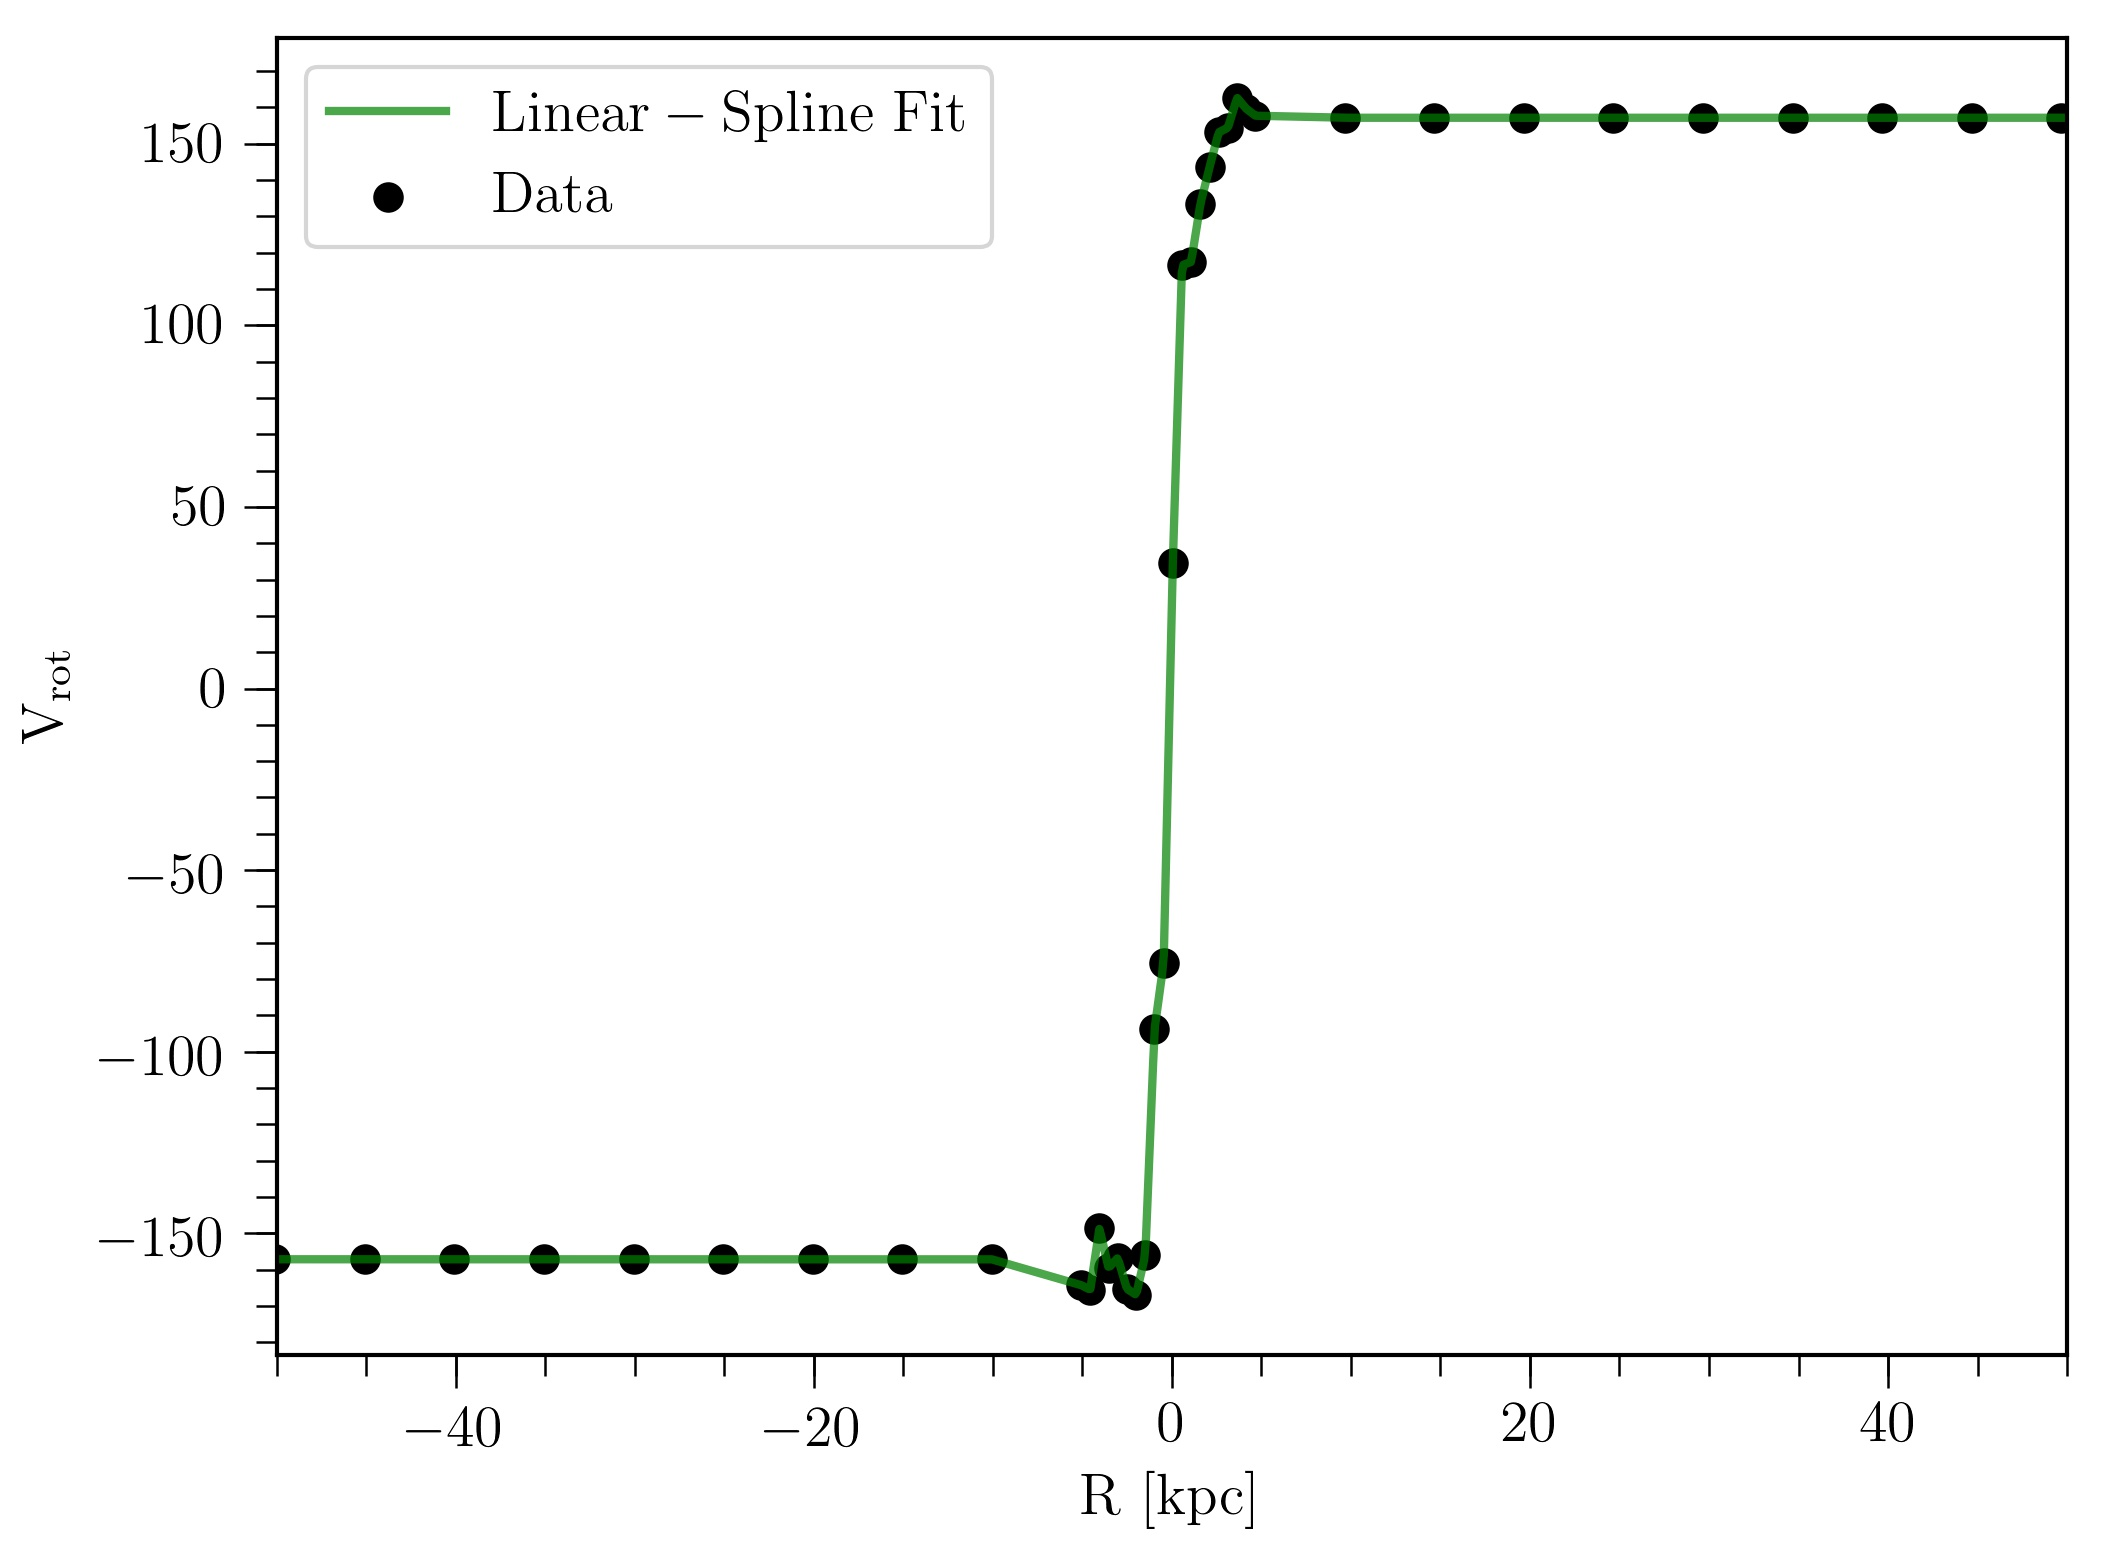
\includegraphics[width=0.36\textwidth]{Chap4/figures/NGC3633_splineFit_linear.jpg}
        \includegraphics[width=0.335\textwidth]{Chap4/figures/NGC3633_2_rotation_curve_xphys_helio_vobs_vrotObs_new5.pdf}
        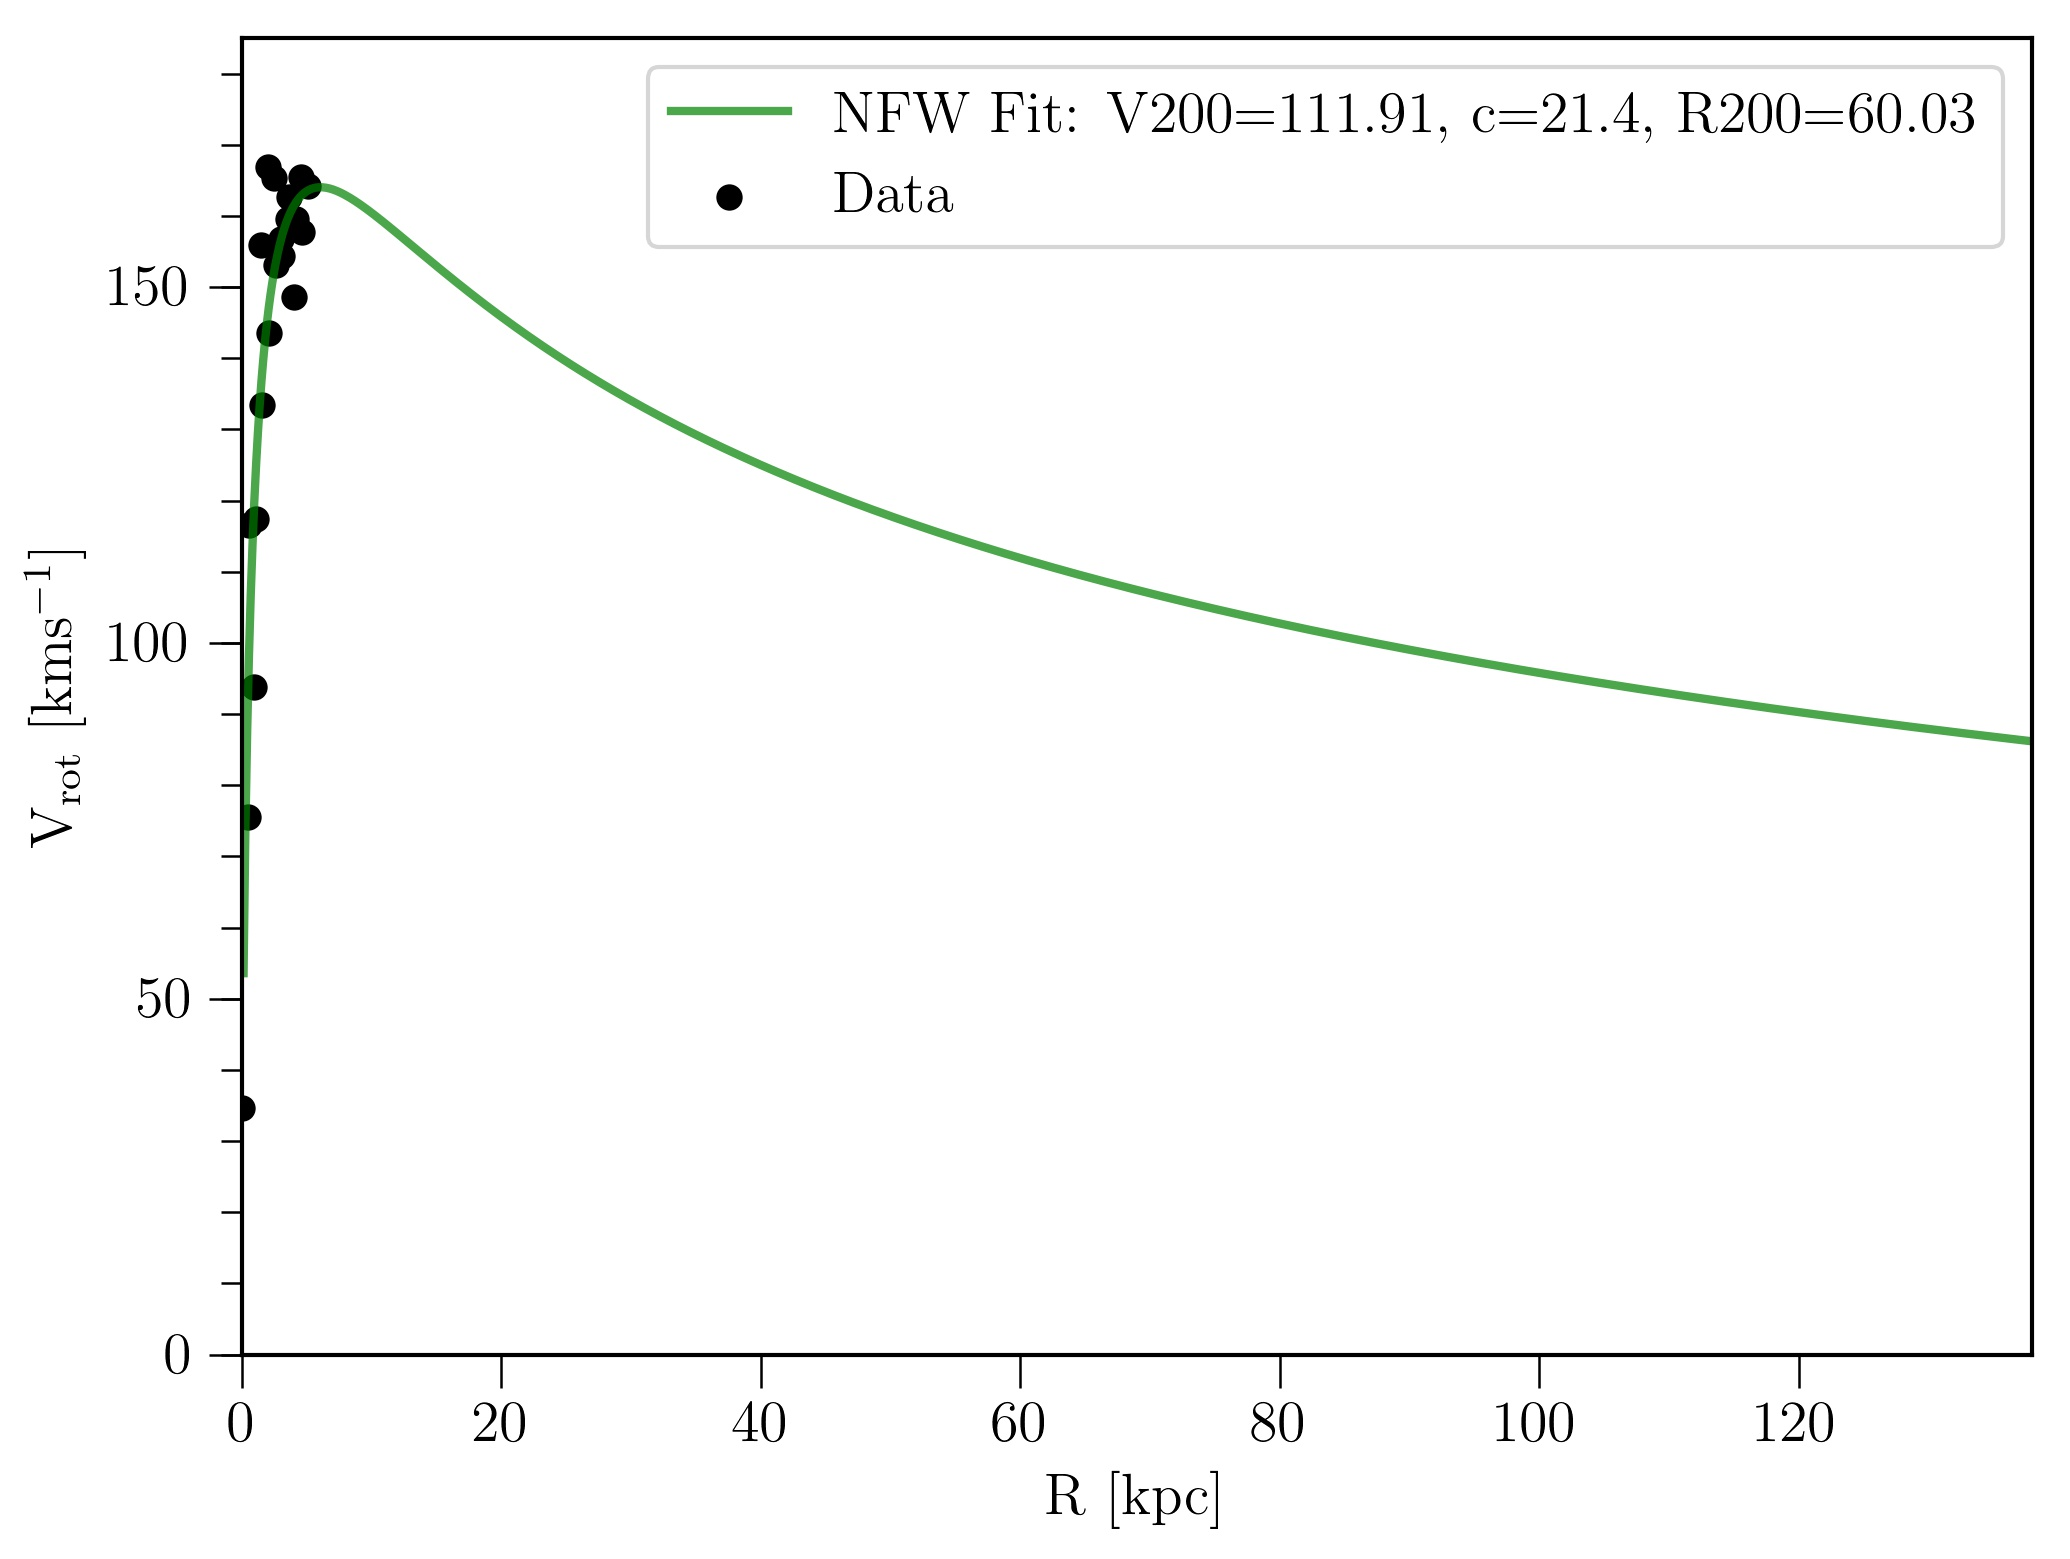
\includegraphics[width=0.33\textwidth]{Chap4/figures/NGC3633_NFW_138.jpg}
        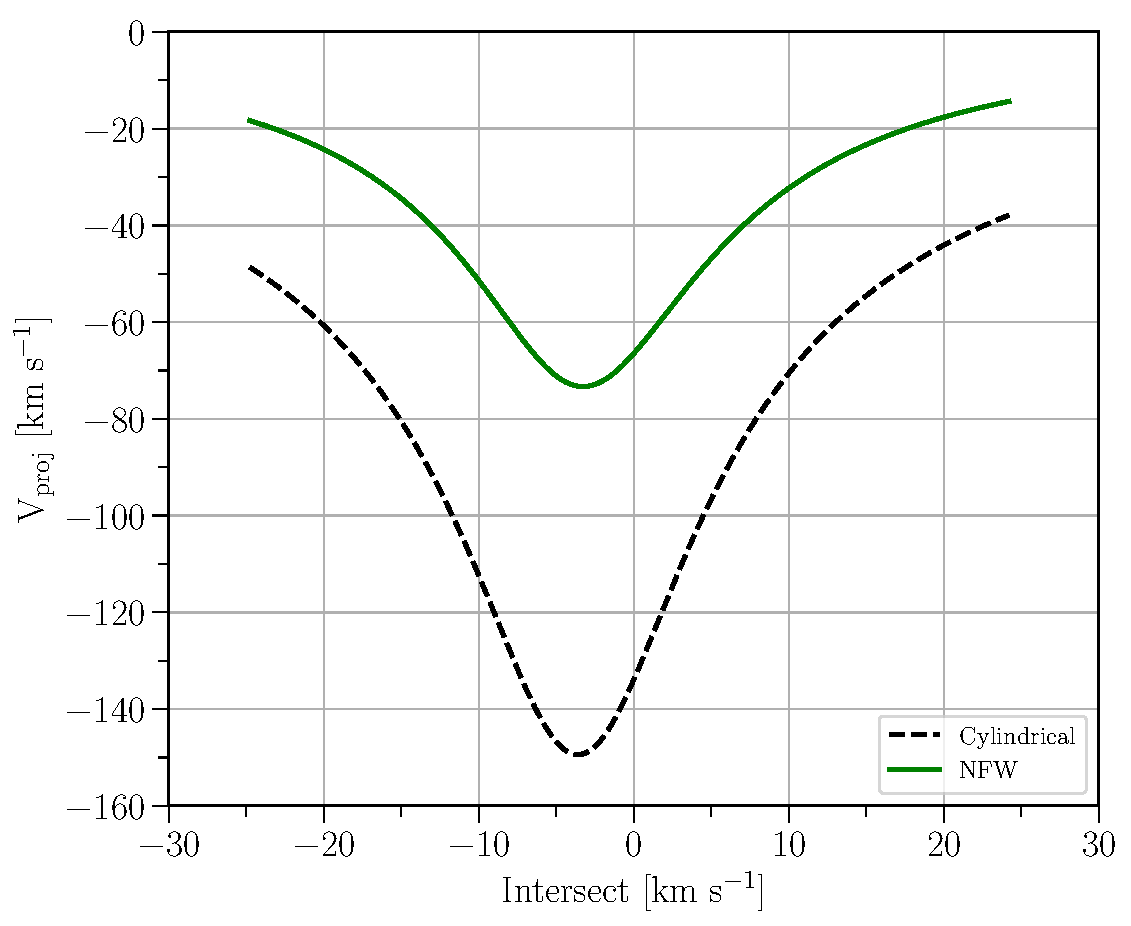
\includegraphics[width=0.31\textwidth]{Chap4/figures/NGC3633-RX_J1121_2+0326_model_plot3.pdf}
        \caption{\small{Left: The rotation curve for NGC3633 is shown in black, with the outer 1/2 mean rotation velocity indicated in green. Our cylindrical model simply extends this green average velocity out to $3 R_{\rm vir}$.  Middle: The observed rotation curve is again shown in black, with an NFW profile fit overlaid in green. Right: The model velocity predictions for the cylindrical and NFW models are shown in dashed-black and solid-green (respectively).}}
%        \vspace{-5pt}
        \label{model_fits}
        \vspace{5pt}
\end{figure}
\begin{figure}[ht!]
        \centering
        \vspace{0pt}
        \includegraphics[width=0.32\textwidth]{Chap4/figures/NGC3633-RX_J1121_2+0326_3Dmodel_plot1_2.pdf}
        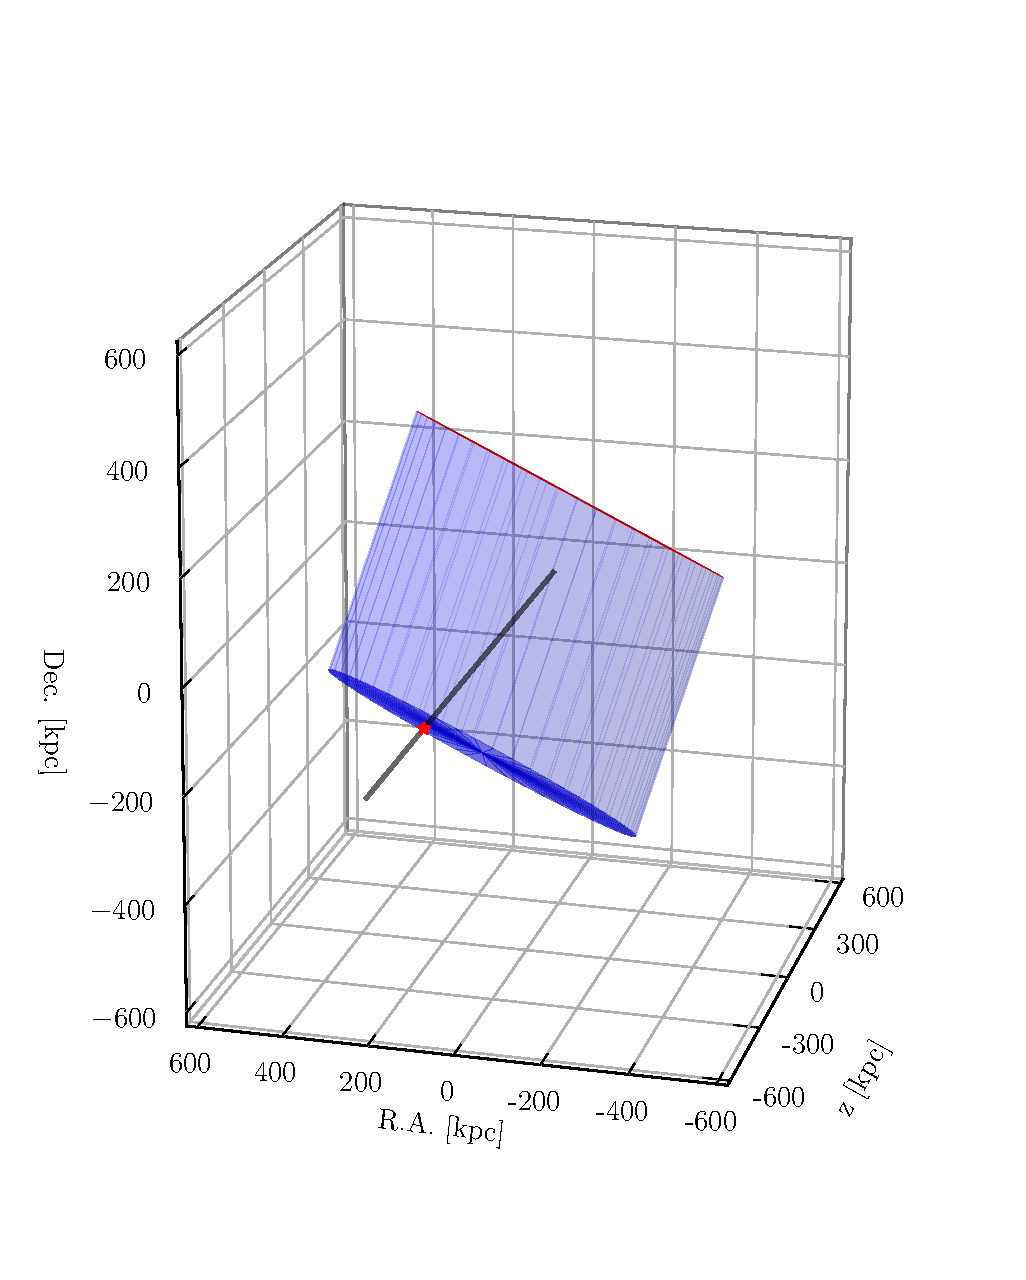
\includegraphics[width=0.32\textwidth]{Chap4/figures/NGC3633-RX_J1121_2+0326_3Dmodel_plot2_2.pdf}
        \includegraphics[width=0.32\textwidth]{Chap4/figures/NGC3633-RX_J1121_2+0326_3Dmodel_plot3_2.pdf}
        \caption{\small{A 3D example mockup of our halo rotation model showing the orientation and extent of the NGC3633 model from 3 different viewing angles. The approaching extreme edge of the NGC3633 cylindrical halo is shown by dark-blue oval, with the far edge shown in red. The dark-grey line shows the location of the sightline toward RX\_J1121.2+0326 as it penetrates the halo, with a red star marking the first intercept point.}}
%        \vspace{-5pt}
        \label{3D_model}
        \vspace{5pt}
\end{figure}
% NFW profile comes from de Blok 2008


\begin{landscape}

% Change the footnote style to lowercase letters
\renewcommand{\thefootnote}{\alph{footnote}}

\scriptsize
\begin{center}
\begin{longtable}{l l l r r r r r r r r}
\caption[CGM Rotation: Halo Model Results and Ly$\alpha$ Absorption Properties]{Halo Model Results and Ly$\alpha$ Absorption Properties} \label{models} \\
\hline \hline \\[-2ex]
  \multicolumn{1}{c}{$\#$} & 
  \multicolumn{1}{c}{Galaxy} &
  \multicolumn{1}{c}{Target} &
  \multicolumn{1}{c}{$\rho$} &
  \multicolumn{1}{c}{Az.} &
  \multicolumn{1}{c}{$v_{\rm sys}$} &
  \multicolumn{1}{c}{$v_{\rm rot}$\tablenotemark{a}} &
  \multicolumn{1}{c}{$v_{\rm Ly\alpha}$} &
  \multicolumn{1}{c}{$W_{\rm Ly\alpha}$} &
  \multicolumn{1}{c}{Cyl. Model\tablenotemark{b}} &
  \multicolumn{1}{c}{NFW Model\tablenotemark{c}} \\
  
  % Units
  \multicolumn{1}{c}{} & 
  \multicolumn{1}{c}{} &
  \multicolumn{1}{c}{} &
  \multicolumn{1}{c}{(kpc)} &
  \multicolumn{1}{c}{(deg)} &
  \multicolumn{1}{c}{(\kms)} &
  \multicolumn{1}{c}{(\kms)} &
  \multicolumn{1}{c}{(\kms)} &
  \multicolumn{1}{c}{$\rm (m\AA)$} &
  \multicolumn{1}{c}{(\kms)} &
  \multicolumn{1}{c}{(\kms)} \\
  
  % column numbers
  \multicolumn{1}{c}{(1)} & 
  \multicolumn{1}{c}{(2)} &
  \multicolumn{1}{c}{(3)} &
  \multicolumn{1}{c}{(4)} &
  \multicolumn{1}{c}{(5)} &
  \multicolumn{1}{c}{(6)} &
  \multicolumn{1}{c}{(7)} &
  \multicolumn{1}{c}{(8)} &
  \multicolumn{1}{c}{(9)} &
  \multicolumn{1}{c}{(10)} &
  \multicolumn{1}{c}{(11)}  \\[0.5ex] \hline \\[-1.8ex]
\endfirsthead

% Second page
\multicolumn{11}{c}{{\tablename} \thetable{} -- Continued} \\[0.5ex]
\hline \hline \\[-2ex]
  \multicolumn{1}{c}{$\#$} & 
  \multicolumn{1}{c}{Galaxy} &
  \multicolumn{1}{c}{Target} &
  \multicolumn{1}{c}{$\rho$} &
  \multicolumn{1}{c}{Az.} &
  \multicolumn{1}{c}{$v_{\rm sys}$} &
  \multicolumn{1}{c}{$v_{\rm rot}$\tablenotemark{a}} &
  \multicolumn{1}{c}{$v_{\rm Ly\alpha}$} &
  \multicolumn{1}{c}{$W_{\rm Ly\alpha}$} &
  \multicolumn{1}{c}{Cyl. Model\tablenotemark{b}} &
  \multicolumn{1}{c}{NFW Model\tablenotemark{c}} \\
  
  % Units
  \multicolumn{1}{c}{} & 
  \multicolumn{1}{c}{} &
  \multicolumn{1}{c}{} &
  \multicolumn{1}{c}{(kpc)} &
  \multicolumn{1}{c}{(deg)} &
  \multicolumn{1}{c}{(\kms)} &
  \multicolumn{1}{c}{(\kms)} &
  \multicolumn{1}{c}{(\kms)} &
  \multicolumn{1}{c}{$\rm (m\AA)$} &
  \multicolumn{1}{c}{(\kms)} &
  \multicolumn{1}{c}{(\kms)} \\
  
  % column numbers
  \multicolumn{1}{c}{(1)} & 
  \multicolumn{1}{c}{(2)} &
  \multicolumn{1}{c}{(3)} &
  \multicolumn{1}{c}{(4)} &
  \multicolumn{1}{c}{(5)} &
  \multicolumn{1}{c}{(6)} &
  \multicolumn{1}{c}{(7)} &
  \multicolumn{1}{c}{(8)} &
  \multicolumn{1}{c}{(9)} &
  \multicolumn{1}{c}{(10)} &
  \multicolumn{1}{c}{(11)}  \\[0.5ex] \hline \\[-1.8ex]
  \endhead

\multicolumn{11}{l}{{Continued on Next Page\ldots}} \\
\endfoot

\\[-1.8ex] \hline \hline
\endlastfoot

%Data starts here:
1  &        CGCG039-137	&	RX\_J1121.2+0326		&         99  &     71  &  6918  &      139  &       6975  &           678  &            6882 - 7055  & 6881 - 7082    \\
2  &        ESO343-G014	&	RBS1768				&                 466  &    74  &  9139  &      205  &       9308  &           63  &             8936 - 9149  & 9017 - 9170    \\
2  &        ESO343-G014	&	RBS1768  			&                 466  &    74  &  9139  &      205  &       9360  &           306  &            8936 - 9149  & 9017 - 9170    \\
2  &        ESO343-G014	&	RBS1768  			&                 466  &    74  &  9139  &      205  &       9434  &           161  &            8936 - 9149  & 9017 - 9170    \\
3  &        IC5325  		&	RBS2000				&                 314  &    64  &  1512  &      -125  &      1598  &           35  &             1471 - 1492  & 1483 - 1513    \\
4  &        MCG-03-58-009	&	MRC2251-178			&             355  &    71  &  9015  &      171  &       9029  &           62  &             8989 - 9152  & 8973 - 9098    \\
5  &        NGC1566		&	1H0419-577  &              303  &    10  &  1502  &      86  &        1075  &           249  &            1550 - 1578  & 1500 - 1533    \\
5  &        NGC1566		&	1H0419-577  &              303  &    10  &  1502  &      86  &        1123  &           269  &            1550 - 1578  & 1500 - 1533    \\
5  &        NGC1566  		&	1H0419-577  &              303  &    10  &  1502  &      86  &        1188  &           240  &            1550 - 1578  & 1500 - 1533    \\
5  &        NGC1566  		&	1H0419-577  &              303  &    10  &  1502  &      86  &        1264  &           91  &             1550 - 1578  & 1500 - 1533    \\
5  &        NGC1566  		&	1H0419-577  &              303  &    10  &  1502  &      86  &        2020  &           9  &              1550 - 1578  & 1500 - 1533    \\
6  &        NGC1566  		&	HE0429-5343  &             256  &    60  &  1502  &      -86  &       1167  &           79  &             1449 - 1500  & 1480 - 1519    \\
6  &        NGC1566  		&	HE0429-5343  &             256  &    60  &  1502  &      -86  &       1358  &           136  &            1449 - 1500  & 1480 - 1519    \\
7  &        NGC2770  		&	FBQSJ0908+3246  &          204  &    59  &  1948  &      150  &       1915  &           202  &            1802 - 1944  & 1831 - 1958    \\
7  &        NGC2770  		&	FBQSJ0908+3246  &          204  &    59  &  1948  &      150  &       1982  &           230  &            1802 - 1944  & 1831 - 1958    \\
8  &        NGC2770  		&	TON1009  &                 267  &    41  &  1948  &      150  &       1908  &           111  &            1802 - 1909  & 1838 - 1934    \\
8  &        NGC2770  		&	TON1009  &                 267  &    41  &  1948  &      150  &       1980  &           243  &            1802 - 1909  & 1838 - 1934    \\
9  &        NGC2770  		&	TON1015  &                 218  &    61  &  1948  &      150  &       1833  &           244  &            1951 - 2094  & 1938 - 2063    \\
9  &        NGC2770  		&	TON1015  &                 218  &    61  &  1948  &      150  &       1985  &           80  &             1951 - 2094  & 1938 - 2063    \\
10  &       NGC2770  		&	SDSSJ091052.80+333008.0  & 239  &    66  &  1948  &      150  &       1824  &           266  &            1954 - 2093  & 1941 - 2060    \\
10  &       NGC2770  		&	SDSSJ091052.80+333008.0  & 239  &    66  &  1948  &      150  &       1975  &           68  &             1954 - 2093  & 1941 - 2060    \\
11  &       NGC2770  		&	SDSSJ091127.30+325337.0  & 234  &    30  &  1948  &      150  &       2063  &           271  &            1798 - 1905  & 1831 - 1929    \\
12  &       NGC3067  		&	3C232  &                   11  &     74  &  1465  &      148.2  &     1408  &           2092  &           1344 - 1490  & 1326 - 1491    \\
12  &       NGC3067  		&	3C232  &                   11  &     74  &  1465  &      148.2  &     1510  &           700  &            1344 - 1490  & 1326 - 1491    \\
12  &       NGC3067  		&	3C232  &                   11  &     74  &  1465  &      148.2  &     1641  &           1635  &           1344 - 1490  & 1326 - 1491    \\
13  &       NGC3067  		&	SDSSJ095914.80+320357.0  & 128  &    43  &  1465  &      148.2  &     1493  &           623  &            1476 - 1603  & 1453 - 1546    \\
14  &       NGC3198 		&	RX\_J1017.5+4702  &         370  &    55  &  660  &       152  &       629  &            71  &             507 - 639  &   569 - 666  \\
15  &       NGC3351  		&	SDSSJ104335.90+115129.0  & 31  &     43  &  778  &       198  &       717  &            823  &            679 - 790  &   710 - 798   \\
15  &       NGC3351  		&	SDSSJ104335.90+115129.0  & 31  &     43  &  778  &       198  &       882  &            621  &            679 - 790  &   710 - 798   \\
15  &       NGC3351  		&	SDSSJ104335.90+115129.0  & 31  &     43  &  778  &       198  &       1030  &           391  &            679 - 790  &   710 - 798  \\
16  &       NGC3432  		&	CSO295  &                  20  &     82  &  616  &       122  &       600  &            568  &            579 - 664  &   579 - 750  \\
16  &       NGC3432  		&	CSO295  &                  20  &     82  &  616  &       122  &       662  &            585  &            579 - 664  &   579 - 750  \\
17  &       NGC3432  		&	RX\_J1054.2+3511  &         290  &    57  &  616  &       122  &       703  &            184  &            616 - 739  &   607 - 727  \\
18  &       NGC3513  		&	H1101-232  &               60  &     67  &  1204  &      20  &        1182  &           635  &            1185 - 1231  & 1185 - 1232    \\
19  &       NGC3631  		&	RX\_J1117.6+5301  &         78  &     75  &  1156  &      145  &       1131  &           374  &            1166 - 1180  & 1157 - 1177    \\
19  &       NGC3631  		&	RX\_J1117.6+5301  &         78  &     75  &  1156  &      145  &       1259  &           62  &             1166 - 1180  & 1157 - 1177    \\
20  &       NGC3631  		&	SBS1116+523  &             163  &    40  &  1156  &      145  &       -99  &            -99  &            1100 - 1151  & 1125 - 1167    \\
21  &       NGC3631  		&	SDSSJ111443.70+525834.0  & 145  &    72  &  1156  &      145  &       1163  &           232  &            1164 - 1185  & 1151 - 1180    \\
22  &       NGC3631  		&	SDSSJ112448.30+531818.0  & 86  &     74  &  1156  &      145  &       1019  &           71  &             1130 - 1145  & 1134 - 1157    \\
22  &       NGC3631  		&	SDSSJ112448.30+531818.0  & 86  &     74  &  1156  &      145  &       1141  &           165  &            1130 - 1145  & 1134 - 1157    \\
23  &       NGC3633  		&	RX\_J1121.2+0326  &         184  &    58  &  2587  &      -157  &      2605  &           180  &            2434 - 2573  & 2510 - 2597    \\
24  &       NGC3666  		&	SDSSJ112439.50+113117.0  & 58  &     83  &  1060  &      131.8  &     1047  &           345  &            973 - 1080  &  924 - 1080   \\
24  &       NGC3666  		&	SDSSJ112439.50+113117.0  & 58  &     83  &  1060  &      131.8  &     1099  &           272  &            973 - 1080  &  924 - 1080  \\
25  &       NGC3726  		&	CSO1208  &                 369  &    88  &  866  &       167.2  &     731  &            470  &            839 - 895  &   838 - 887  \\
25  &       NGC3726  		&	CSO1208  &                 369  &    88  &  866  &       167.2  &     874  &            506  &            839 - 895  &   838 - 887   \\
26  &       NGC3726  		&	RX\_J1142.7+4625  &         440  &    86  &  866  &       167.2  &     818  &            375  &            832 - 852  &   836 - 859   \\
27  &       NGC4529  		&	MRK771  &                  159  &    23  &  2536  &      106.4  &     2553  &           240  &            2433 - 2496  & 2449 - 2511    \\
28  &       NGC4536  		&	3C273.0  &                 349  &    11  &  1867  &      139  &       1580  &           369  &            1954 - 1988  & 1872 - 1908    \\
28  &       NGC4536  		&	3C273.0  &                 349  &    11  &  1867  &      139  &       2156  &           42  &             1954 - 1988  & 1872 - 1908    \\
28  &       NGC4536  		&	3C273.0  &                 349  &    11  &  1867  &      139  &       2267  &           27  &             1954 - 1988  & 1872 - 1908    \\
29  &       NGC4536  		&	HE1228+0131  &             338  &    51  &  1867  &      139  &       1495  &           160  &            1885 - 1918  & 1869 - 1899    \\
29  &       NGC4536  		&	HE1228+0131  &             338  &    51  &  1867  &      139  &       1571  &           23  &             1885 - 1918  & 1869 - 1899    \\
29  &       NGC4536  		&	HE1228+0131  &             338  &    51  &  1867  &      139  &       1686  &           321  &            1885 - 1918  & 1869 - 1899    \\
29  &       NGC4536  		&	HE1228+0131  &             338  &    51  &  1867  &      139  &       1721  &           303  &            1885 - 1918  & 1869 - 1899    \\
29  &       NGC4536  		&	HE1228+0131  &             338  &    51  &  1867  &      139  &       1854  &           78  &             1885 - 1918  & 1869 - 1899    \\
30  &       NGC4565  		&	RX\_J1236.0+2641  &         147  &    41  &  1230  &      253  &       1009  &           365  &            1228 - 1476  & 1200 - 1374    \\
30  &       NGC4565  		&	RX\_J1236.0+2641  &         147  &    41  &  1230  &      253  &       1166  &           305  &            1228 - 1476  & 1200 - 1374    \\
30  &       NGC4565  		&	RX\_J1236.0+2641  &         147  &    41  &  1230  &      253  &       1254  &           122  &            1228 - 1476  & 1200 - 1374    \\
31  &       NGC4939  		&	PG1302-102  &              254  &    61  &  3093  &      -275  &      3448  &           72  &             2874 - 3107  & 2974 - 3129    \\
32  &       NGC5364  		&	SDSSJ135726.27+043541.4  & 165  &    84  &  1238  &      55  &        967  &            348  &            1212 - 1346  & 1208 - 1306    \\
32  &       NGC5364  		&	SDSSJ135726.27+043541.4  & 165  &    84  &  1238  &      55  &        1124  &           83  &             1212 - 1346  & 1208 - 1306    \\
33  &       NGC5786  		&	QSO1500-4140  &            453  &    1  &   2975  &      172  &       3138  &           177  &            3081 - 3135  & 2994 - 3042    \\
34  &       NGC5907  		&	SBS1503+570  &             413  &    47  &  667  &       227.4  &     708  &            301  &            698 - 895  &   643 - 768   \\
35  &       NGC5907  		&	RBS1503  &                 478  &    63  &  667  &       227.4  &     -99  &            -99  &            439 - 658  &   571 - 700  \\
36  &       NGC5951  		&	2E1530+1511  &             55  &     85  &  1780  &      127.9  &     1795  &           507  &            1749 - 1894  & 1748 - 1905    \\
36  &       NGC5951  		&	2E1530+1511  &             55  &     85  &  1780  &      127.9  &     1953  &           137  &            1749 - 1894  & 1748 - 1905    \\
37  &       NGC6140  		&	MRK876  &                  113  &    21  &  910  &       138.11  &    939  &            379  &            950 - 1011  &  945 - 1012  \\
38  &       NGC7817  		&	MRK335  &                  343  &    90  &  2309  &      180.4  &     1954  &           216  &            2283 - 2285  & 2283 - 2285    \\
38  &       NGC7817  		&	MRK335  &                  343  &    90  &  2309  &      180.4  &     2274  &           150  &            2283 - 2285  & 2283 - 2285    \\
39  &       UGC04238  	&      PG0804+761  &              148  &    59  &  1544  &      91.6  &      1526  &           62  &             1541 - 1630  & 1534 - 1619    \\
39  &       UGC04238  	&      PG0804+761  &              148  &    59  &  1544  &      91.6  &      1593  &           32  &             1541 - 1630  & 1534 - 1619    \\
40  &       UGC06446  	&      SDSSJ112448.30+531818.0  & 143  &    22  &  645  &       79.4  &      664  &            339  &            636 - 710  &   630 - 706  \\
41  &       UGC08146  	&      PG1259+593  &              114  &    50  &  670  &       82.4  &      646  &            133  &            657 - 752  &   654 - 753  \\
41  &       UGC08146  	&      PG1259+593  &              114  &    50  &  670  &       82.4  &      683  &            168  &            657 - 752  &   654 - 753   \\
42  &       UGC09760  	&      SDSSJ151237.15+012846.0  & 123  &    90  &  2094  &      -46  &       2029  &           506  &            2064 - 2124  & 2064 - 2180    \\

% footnote a:
\footnotetext[1]{Galaxy rotation velocity in the direction of the target in column 3.} 
\footnotetext[2]{Range of heliocentric velocities consistent with cylindrical co-rotation from the location of the target in column 3.} 
\footnotetext[3]{Range of heliocentric velocities consistent with NFW halo co-rotation from the location of the target in column 3.}

\end{longtable}
\end{center}
\normalsize

% Reset the footnotes back to numbers
\renewcommand{\thefootnote}{\arabic{}}

\end{landscape}


%\begin{deluxetable}{l l l r r r r r r r r}
%\rotate
%\tabletypesize{\footnotesize}
%\tablewidth{0pt}
%\tablecaption{Halo Model Results and Ly$\alpha$ Absorption Properties\label{models}}
%\tablehead{
%\colhead{$\#$}	&\colhead{Galaxy}  	&  \colhead{Target} 	&  \colhead{$\rho$ }  &  \colhead{Az.}      & \colhead{$v_{\rm sys}$}&  \colhead{$v_{\rm rot}$\tablenotemark{a}}   &  \colhead{$v_{\rm Ly\alpha}$} & \colhead{$W_{\rm Ly\alpha}$} & \colhead{Cyl. Model\tablenotemark{b}}  & \colhead{NFW Model\tablenotemark{c}}  \\
%			  				&				&          			&  \colhead{(kpc)}   & \colhead{(deg)}	& \colhead{(\kms)}	     & \colhead{(\kms)}  		& \colhead{(\kms)}  		      	&  \colhead{(m\AA)}  			  & \colhead{(\kms)} 	       & \colhead{(\kms)} }
%\startdata
%1  &        CGCG039-137	&	RX\_J1121.2+0326		&         99  &     71  &  6918  &      139  &       6975  &           678  &            6882 - 7055  & 6881 - 7082    \\
%2  &        ESO343-G014	&	RBS1768				&                 466  &    74  &  9139  &      205  &       9308  &           63  &             8936 - 9149  & 9017 - 9170    \\
%2  &        ESO343-G014	&	RBS1768  			&                 466  &    74  &  9139  &      205  &       9360  &           306  &            8936 - 9149  & 9017 - 9170    \\
%2  &        ESO343-G014	&	RBS1768  			&                 466  &    74  &  9139  &      205  &       9434  &           161  &            8936 - 9149  & 9017 - 9170    \\
%3  &        IC5325  		&	RBS2000				&                 314  &    64  &  1512  &      -125  &      1598  &           35  &             1471 - 1492  & 1483 - 1513    \\
%4  &        MCG-03-58-009	&	MRC2251-178			&             355  &    71  &  9015  &      171  &       9029  &           62  &             8989 - 9152  & 8973 - 9098    \\
%5  &        NGC1566		&	1H0419-577  &              303  &    10  &  1502  &      86  &        1075  &           249  &            1550 - 1578  & 1500 - 1533    \\
%5  &        NGC1566		&	1H0419-577  &              303  &    10  &  1502  &      86  &        1123  &           269  &            1550 - 1578  & 1500 - 1533    \\
%5  &        NGC1566  		&	1H0419-577  &              303  &    10  &  1502  &      86  &        1188  &           240  &            1550 - 1578  & 1500 - 1533    \\
%5  &        NGC1566  		&	1H0419-577  &              303  &    10  &  1502  &      86  &        1264  &           91  &             1550 - 1578  & 1500 - 1533    \\
%5  &        NGC1566  		&	1H0419-577  &              303  &    10  &  1502  &      86  &        2020  &           9  &              1550 - 1578  & 1500 - 1533    \\
%6  &        NGC1566  		&	HE0429-5343  &             256  &    60  &  1502  &      -86  &       1167  &           79  &             1449 - 1500  & 1480 - 1519    \\
%6  &        NGC1566  		&	HE0429-5343  &             256  &    60  &  1502  &      -86  &       1358  &           136  &            1449 - 1500  & 1480 - 1519    \\
%7  &        NGC2770  		&	FBQSJ0908+3246  &          204  &    59  &  1948  &      150  &       1915  &           202  &            1802 - 1944  & 1831 - 1958    \\
%7  &        NGC2770  		&	FBQSJ0908+3246  &          204  &    59  &  1948  &      150  &       1982  &           230  &            1802 - 1944  & 1831 - 1958    \\
%8  &        NGC2770  		&	TON1009  &                 267  &    41  &  1948  &      150  &       1908  &           111  &            1802 - 1909  & 1838 - 1934    \\
%8  &        NGC2770  		&	TON1009  &                 267  &    41  &  1948  &      150  &       1980  &           243  &            1802 - 1909  & 1838 - 1934    \\
%9  &        NGC2770  		&	TON1015  &                 218  &    61  &  1948  &      150  &       1833  &           244  &            1951 - 2094  & 1938 - 2063    \\
%9  &        NGC2770  		&	TON1015  &                 218  &    61  &  1948  &      150  &       1985  &           80  &             1951 - 2094  & 1938 - 2063    \\
%10  &       NGC2770  		&	SDSSJ091052.80+333008.0  & 239  &    66  &  1948  &      150  &       1824  &           266  &            1954 - 2093  & 1941 - 2060    \\
%10  &       NGC2770  		&	SDSSJ091052.80+333008.0  & 239  &    66  &  1948  &      150  &       1975  &           68  &             1954 - 2093  & 1941 - 2060    \\
%11  &       NGC2770  		&	SDSSJ091127.30+325337.0  & 234  &    30  &  1948  &      150  &       2063  &           271  &            1798 - 1905  & 1831 - 1929    \\
%12  &       NGC3067  		&	3C232  &                   11  &     74  &  1465  &      148.2  &     1408  &           2092  &           1344 - 1490  & 1326 - 1491    \\
%12  &       NGC3067  		&	3C232  &                   11  &     74  &  1465  &      148.2  &     1510  &           700  &            1344 - 1490  & 1326 - 1491    \\
%12  &       NGC3067  		&	3C232  &                   11  &     74  &  1465  &      148.2  &     1641  &           1635  &           1344 - 1490  & 1326 - 1491    \\
%13  &       NGC3067  		&	SDSSJ095914.80+320357.0  & 128  &    43  &  1465  &      148.2  &     1493  &           623  &            1476 - 1603  & 1453 - 1546    \\
%14  &       NGC3198 		&	RX\_J1017.5+4702  &         370  &    55  &  660  &       152  &       629  &            71  &             507 - 639  &   569 - 666  \\
%15  &       NGC3351  		&	SDSSJ104335.90+115129.0  & 31  &     43  &  778  &       198  &       717  &            823  &            679 - 790  &   710 - 798   \\
%15  &       NGC3351  		&	SDSSJ104335.90+115129.0  & 31  &     43  &  778  &       198  &       882  &            621  &            679 - 790  &   710 - 798   \\
%15  &       NGC3351  		&	SDSSJ104335.90+115129.0  & 31  &     43  &  778  &       198  &       1030  &           391  &            679 - 790  &   710 - 798  \\
%16  &       NGC3432  		&	CSO295  &                  20  &     82  &  616  &       122  &       600  &            568  &            579 - 664  &   579 - 750  \\
%16  &       NGC3432  		&	CSO295  &                  20  &     82  &  616  &       122  &       662  &            585  &            579 - 664  &   579 - 750  \\
%17  &       NGC3432  		&	RX\_J1054.2+3511  &         290  &    57  &  616  &       122  &       703  &            184  &            616 - 739  &   607 - 727  \\
%18  &       NGC3513  		&	H1101-232  &               60  &     67  &  1204  &      20  &        1182  &           635  &            1185 - 1231  & 1185 - 1232    \\
%19  &       NGC3631  		&	RX\_J1117.6+5301  &         78  &     75  &  1156  &      145  &       1131  &           374  &            1166 - 1180  & 1157 - 1177    \\
%19  &       NGC3631  		&	RX\_J1117.6+5301  &         78  &     75  &  1156  &      145  &       1259  &           62  &             1166 - 1180  & 1157 - 1177    \\
%20  &       NGC3631  		&	SBS1116+523  &             163  &    40  &  1156  &      145  &       -99  &            -99  &            1100 - 1151  & 1125 - 1167    \\
%21  &       NGC3631  		&	SDSSJ111443.70+525834.0  & 145  &    72  &  1156  &      145  &       1163  &           232  &            1164 - 1185  & 1151 - 1180    \\
%22  &       NGC3631  		&	SDSSJ112448.30+531818.0  & 86  &     74  &  1156  &      145  &       1019  &           71  &             1130 - 1145  & 1134 - 1157    \\
%22  &       NGC3631  		&	SDSSJ112448.30+531818.0  & 86  &     74  &  1156  &      145  &       1141  &           165  &            1130 - 1145  & 1134 - 1157    \\
%23  &       NGC3633  		&	RX\_J1121.2+0326  &         184  &    58  &  2587  &      -157  &      2605  &           180  &            2434 - 2573  & 2510 - 2597    \\
%24  &       NGC3666  		&	SDSSJ112439.50+113117.0  & 58  &     83  &  1060  &      131.8  &     1047  &           345  &            973 - 1080  &  924 - 1080   \\
%24  &       NGC3666  		&	SDSSJ112439.50+113117.0  & 58  &     83  &  1060  &      131.8  &     1099  &           272  &            973 - 1080  &  924 - 1080  \\
%25  &       NGC3726  		&	CSO1208  &                 369  &    88  &  866  &       167.2  &     731  &            470  &            839 - 895  &   838 - 887  \\
%25  &       NGC3726  		&	CSO1208  &                 369  &    88  &  866  &       167.2  &     874  &            506  &            839 - 895  &   838 - 887   \\
%26  &       NGC3726  		&	RX\_J1142.7+4625  &         440  &    86  &  866  &       167.2  &     818  &            375  &            832 - 852  &   836 - 859   \\
%27  &       NGC4529  		&	MRK771  &                  159  &    23  &  2536  &      106.4  &     2553  &           240  &            2433 - 2496  & 2449 - 2511    \\
%28  &       NGC4536  		&	3C273.0  &                 349  &    11  &  1867  &      139  &       1580  &           369  &            1954 - 1988  & 1872 - 1908    \\
%28  &       NGC4536  		&	3C273.0  &                 349  &    11  &  1867  &      139  &       2156  &           42  &             1954 - 1988  & 1872 - 1908    \\
%28  &       NGC4536  		&	3C273.0  &                 349  &    11  &  1867  &      139  &       2267  &           27  &             1954 - 1988  & 1872 - 1908    \\
%29  &       NGC4536  		&	HE1228+0131  &             338  &    51  &  1867  &      139  &       1495  &           160  &            1885 - 1918  & 1869 - 1899    \\
%29  &       NGC4536  		&	HE1228+0131  &             338  &    51  &  1867  &      139  &       1571  &           23  &             1885 - 1918  & 1869 - 1899    \\
%29  &       NGC4536  		&	HE1228+0131  &             338  &    51  &  1867  &      139  &       1686  &           321  &            1885 - 1918  & 1869 - 1899    \\
%29  &       NGC4536  		&	HE1228+0131  &             338  &    51  &  1867  &      139  &       1721  &           303  &            1885 - 1918  & 1869 - 1899    \\
%29  &       NGC4536  		&	HE1228+0131  &             338  &    51  &  1867  &      139  &       1854  &           78  &             1885 - 1918  & 1869 - 1899    \\
%30  &       NGC4565  		&	RX\_J1236.0+2641  &         147  &    41  &  1230  &      253  &       1009  &           365  &            1228 - 1476  & 1200 - 1374    \\
%30  &       NGC4565  		&	RX\_J1236.0+2641  &         147  &    41  &  1230  &      253  &       1166  &           305  &            1228 - 1476  & 1200 - 1374    \\
%30  &       NGC4565  		&	RX\_J1236.0+2641  &         147  &    41  &  1230  &      253  &       1254  &           122  &            1228 - 1476  & 1200 - 1374    \\
%31  &       NGC4939  		&	PG1302-102  &              254  &    61  &  3093  &      -275  &      3448  &           72  &             2874 - 3107  & 2974 - 3129    \\
%32  &       NGC5364  		&	SDSSJ135726.27+043541.4  & 165  &    84  &  1238  &      55  &        967  &            348  &            1212 - 1346  & 1208 - 1306    \\
%32  &       NGC5364  		&	SDSSJ135726.27+043541.4  & 165  &    84  &  1238  &      55  &        1124  &           83  &             1212 - 1346  & 1208 - 1306    \\
%33  &       NGC5786  		&	QSO1500-4140  &            453  &    1  &   2975  &      172  &       3138  &           177  &            3081 - 3135  & 2994 - 3042    \\
%34  &       NGC5907  		&	SBS1503+570  &             413  &    47  &  667  &       227.4  &     708  &            301  &            698 - 895  &   643 - 768   \\
%35  &       NGC5907  		&	RBS1503  &                 478  &    63  &  667  &       227.4  &     -99  &            -99  &            439 - 658  &   571 - 700  \\
%36  &       NGC5951  		&	2E1530+1511  &             55  &     85  &  1780  &      127.9  &     1795  &           507  &            1749 - 1894  & 1748 - 1905    \\
%36  &       NGC5951  		&	2E1530+1511  &             55  &     85  &  1780  &      127.9  &     1953  &           137  &            1749 - 1894  & 1748 - 1905    \\
%37  &       NGC6140  		&	MRK876  &                  113  &    21  &  910  &       138.11  &    939  &            379  &            950 - 1011  &  945 - 1012  \\
%38  &       NGC7817  		&	MRK335  &                  343  &    90  &  2309  &      180.4  &     1954  &           216  &            2283 - 2285  & 2283 - 2285    \\
%38  &       NGC7817  		&	MRK335  &                  343  &    90  &  2309  &      180.4  &     2274  &           150  &            2283 - 2285  & 2283 - 2285    \\
%39  &       UGC04238  	&      PG0804+761  &              148  &    59  &  1544  &      91.6  &      1526  &           62  &             1541 - 1630  & 1534 - 1619    \\
%39  &       UGC04238  	&      PG0804+761  &              148  &    59  &  1544  &      91.6  &      1593  &           32  &             1541 - 1630  & 1534 - 1619    \\
%40  &       UGC06446  	&      SDSSJ112448.30+531818.0  & 143  &    22  &  645  &       79.4  &      664  &            339  &            636 - 710  &   630 - 706  \\
%41  &       UGC08146  	&      PG1259+593  &              114  &    50  &  670  &       82.4  &      646  &            133  &            657 - 752  &   654 - 753  \\
%41  &       UGC08146  	&      PG1259+593  &              114  &    50  &  670  &       82.4  &      683  &            168  &            657 - 752  &   654 - 753   \\
%42  &       UGC09760  	&      SDSSJ151237.15+012846.0  & 123  &    90  &  2094  &      -46  &       2029  &           506  &            2064 - 2124  & 2064 - 2180    \\
%\enddata
%\tablecomments{
%\tablenotetext{a}{Galaxy rotation velocity in the direction of the target in column 3.} 
%\tablenotetext{b}{Range of heliocentric velocities consistent with cylindrical co-rotation from the location of the target in column 3.} 
%\tablenotetext{c}{Range of heliocentric velocities consistent with NFW halo co-rotation from the location of the target in column 3.} }
%\end{deluxetable}


\section{Discussion} \label{discussion}
We present data on 41 QSO systems, representing 65 individual Ly$\rm \alpha$ component-galaxy matchups, for which we have galaxy information including kinematics, inclination, size and luminosity. This is the largest sample of this kind to date and provides the best yet opportunity to study the kinematic connection between galaxies and their neutral \HI~halos. 

Table \ref{results} summarizes our galaxy-absorber sample and the predicted velocity range given by each model for co-rotation. Unfortunately our sample contains a large number of high-azimuth targets (i.e., the QSO lies close to the projected galaxy minor axis). These high-azimuth systems are inherently uncertain. For even the most edge-on galaxies, reasonable values for the position angle can vary by at least $\sim 5^{\circ}$, and this becomes even more uncertain for lower inclination galaxies. Because of this inherent uncertainty in every position angle measurement, we have automatically designated every system with an azimuth of $85^{\circ}$ or higher as ``uncertain." We do not include these when calculating co-rotation fractions or otherwise separating systems into co- and anti-rotating subsets. 

For the remaining sample we designate each system as co-rotating or anti-rotating firstly based on the on-sky apparent velocity orientation. For example, an absorber with positive $\Delta v$ which is detected on the receding side of a galaxy is labeled ``co-rotating" (recall $\Delta v = v_{\rm absorber} - v_{\rm galaxy}$, hence a positive value corresponds to absorption with velocity higher than the galaxy systemic). Next, we compare $\Delta v$ of each absorber to our cylindrical and NFW profile fit model predictions. For example, an absorber with $\Delta v = 50$ and model ranges of (cylindrical = [0, 35], NFW = [10, 55]) would be labeled ``anti-rotating" for the cylindrical and ``co-rotating" for the NFW models, because $\Delta v = 50$ \kms~is inside the NFW range and outside the cylindrical range. In order to broadly account for both velocity uncertainties and absorber linewidth, we allow for an $\pm 10$ \kms~error with respect to these model ranges (i.e., if $\Delta v$ is within 10 \kms~of the edge of either model velocity range we count it as ``co-rotating"). This is a conservative underestimate of the true errors in the sense that larger errors would allow for \emph{more} absorbers to be labeled ``co-rotating." The majority of our ``co-rotating" sample fall well within the model ranges, so few would be thrown into uncertainty with a larger error, whereas many ``anti-rotators" are close to the allowed ranges.

\subsection{Co-rotation Fraction}
Here we consider in aggregate our sample of Ly$\alpha$ absorbers, and the fraction consistent with co-rotation under various cuts and constraints. 

To start we consider the fraction of absorbers which appear to be rotating in the same sense as the nearby galaxy. With no cuts of any kind, we find 54\% of absorbers to be co-rotating with the nearby galaxy based on apparent velocity only. Figure \ref{full_map} presents an map of the locations of each absorber relative to it's assumed host galaxy. In this figure we have rotated every system such that the galaxy major axes are horizontal with the approaching side on the left. Blue-diamonds indicate the absorber has the appropriate velocity sign for co-rotation, red-crosses indicate an anti-alignment, grey circles indicate uncertain systems due to their high azimuth angles, and open grey circles indicate non-detections. We have also scaled the size of each marker according to it's relative EW, and annotated each with a number corresponding to the appropriate system number given in Column (1) of Table \ref{models}. Figure \ref{zoom_map} shows the same map zoomed in to a radius of $1 R_{\rm vir}$.

%\begin{figure}[ht!]
%        \centering
%        \vspace{0pt}
%        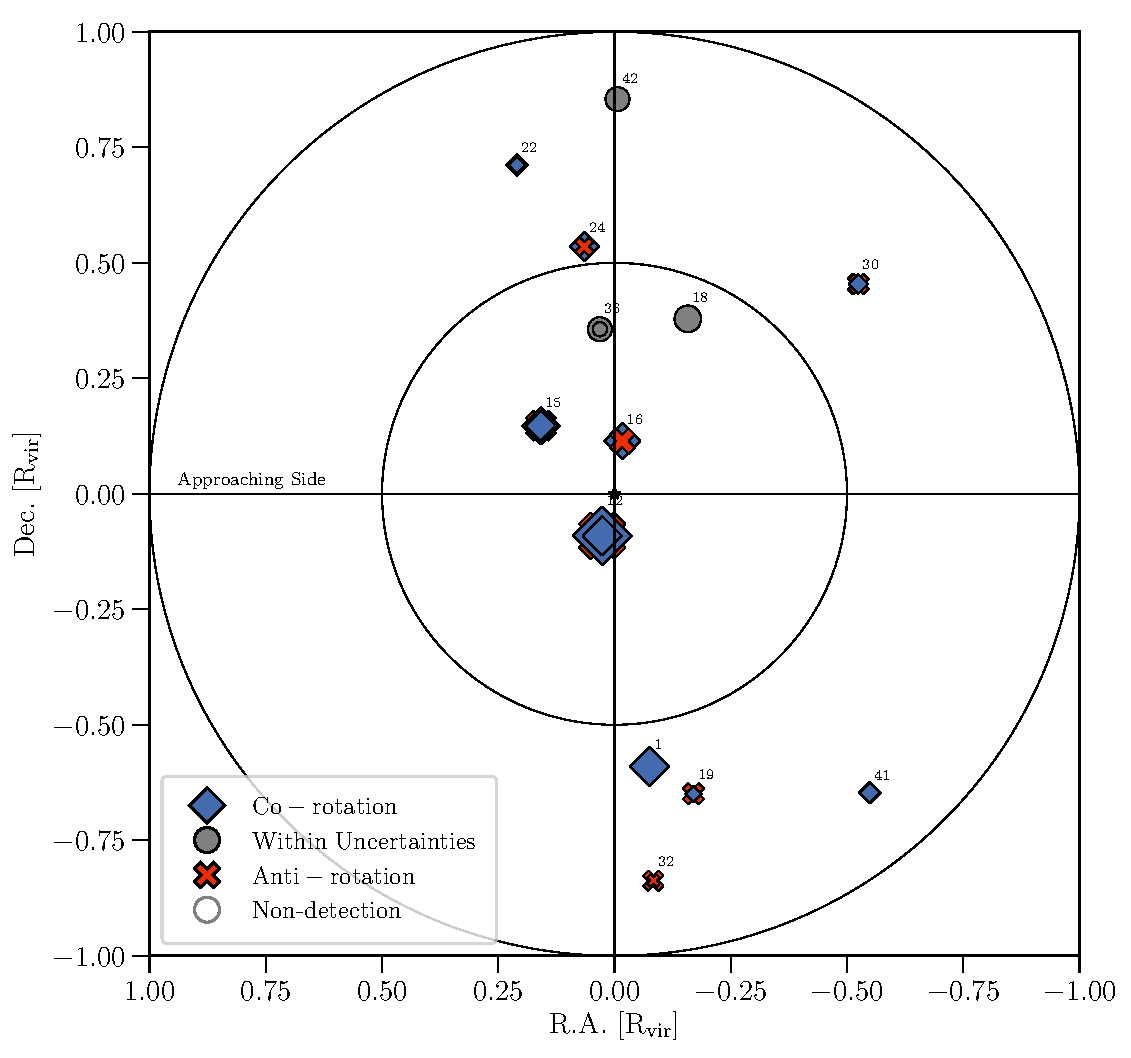
\includegraphics[width=0.5\textwidth]{Chap4/figures/SALTmap_velstrict_False_non_True_Lstar_0-100_minsep_False_zoom_10_inclim_00.pdf}
%        \caption{\small{A map of the locations of each absorber normalized with respect to the galaxy virial radius, showing only those systems within $1 R_{\rm vir}$. The color and style of each point indicates the line-of-sight velocity compared to that of the rotation of the nearby galaxy. Blue diamonds indicate co-rotation, red crosses indicate anti-rotation, and grey circles indicate cases where either is possible due to a combination of orientation and velocity uncertainties. The size of each point is scaled to reflect the EW of the absorber. Concentric rings indicate distances of 0.5 and 1 $R_{vir}$. All galaxies are rotated to PA = 90 or 270, such that their major axis' are horizontal and their approaching side is on the left as indicated. The number identifiers correspond to the system number given in column (1) of Table \ref{model}.}}
%        \vspace{-5pt}
%        \label{zoom_map}
%\end{figure}
%\begin{figure}[ht!]
%        \centering
%        \vspace{0pt}
%        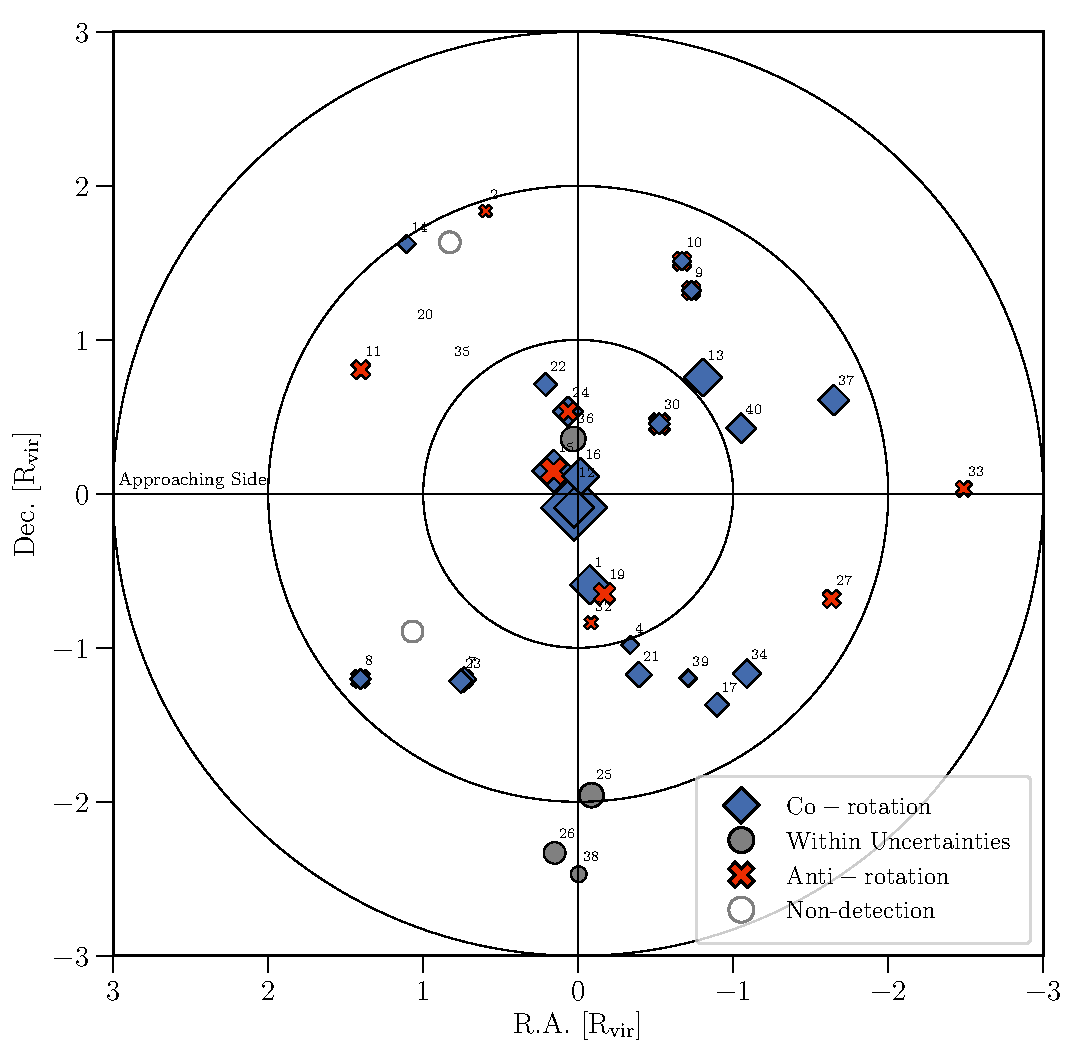
\includegraphics[width=0.48\textwidth]{Chap4/figures/SALTmap_NFW_model_velstrict_True_non_True_Lstar_0-100_minsep_False_inclim_00.pdf}
%        \caption{\small{A map of the locations of each absorber normalized with respect to the galaxy virial radius. The color and style of each point indicates the NFW rotation model results for each absorber with a $v_{\rm Ly\alpha} \leq v_{\rm rot}$ constraint imposed. Blue diamonds indicate co-rotation, red crosses indicate anti-rotation, and grey circles indicate cases where either is possible due to a combination of orientation and velocity uncertainties. The size of each point is scaled to reflect the EW of the absorber. Concentric rings indicate distances of 1, 2, and 3 $R_{vir}$. All galaxies are rotated to PA = 90 or 270, such that their major axis' are horizontal and their approaching side is on the left as indicated. The number identifiers correspond to the system number given in column (1) of Table \ref{model}.}}
%%        \vspace{-5pt}
%        \label{nfw_map}
%\end{figure}


\begin{figure}[ht!]
        \centering
        \vspace{0pt}
        \includegraphics[width=0.84\textwidth]{Chap4/figures/SALTmap_velstrict_False_non_True_Lstar_0-100_minsep_False_inclim_0.pdf}
        \caption{\small{A map of the locations of each absorber normalized with respect to the galaxy virial radius, with \emph{no} additional constraints. The color and style of each point indicates the line-of-sight velocity compared to that of the rotation of the nearby galaxy. Blue diamonds indicate co-rotation, red crosses indicate anti-rotation, and grey circles indicate cases where either is possible due to a combination of orientation and velocity uncertainties. The size of each point is scaled to reflect the EW of the absorber. Concentric rings indicate distances of 1, 2, and 3 $R_{\rm vir}$. All galaxies are rotated to PA = 90 or 270, such that their major axis' are horizontal and their approaching side is on the left as indicated. The number identifiers correspond to the system number given in column (1) of Table \ref{model}.}}
%        \vspace{5pt}
        \label{full_map}
\end{figure}

\begin{figure}[ht!]
\centering
  \subfigure[]{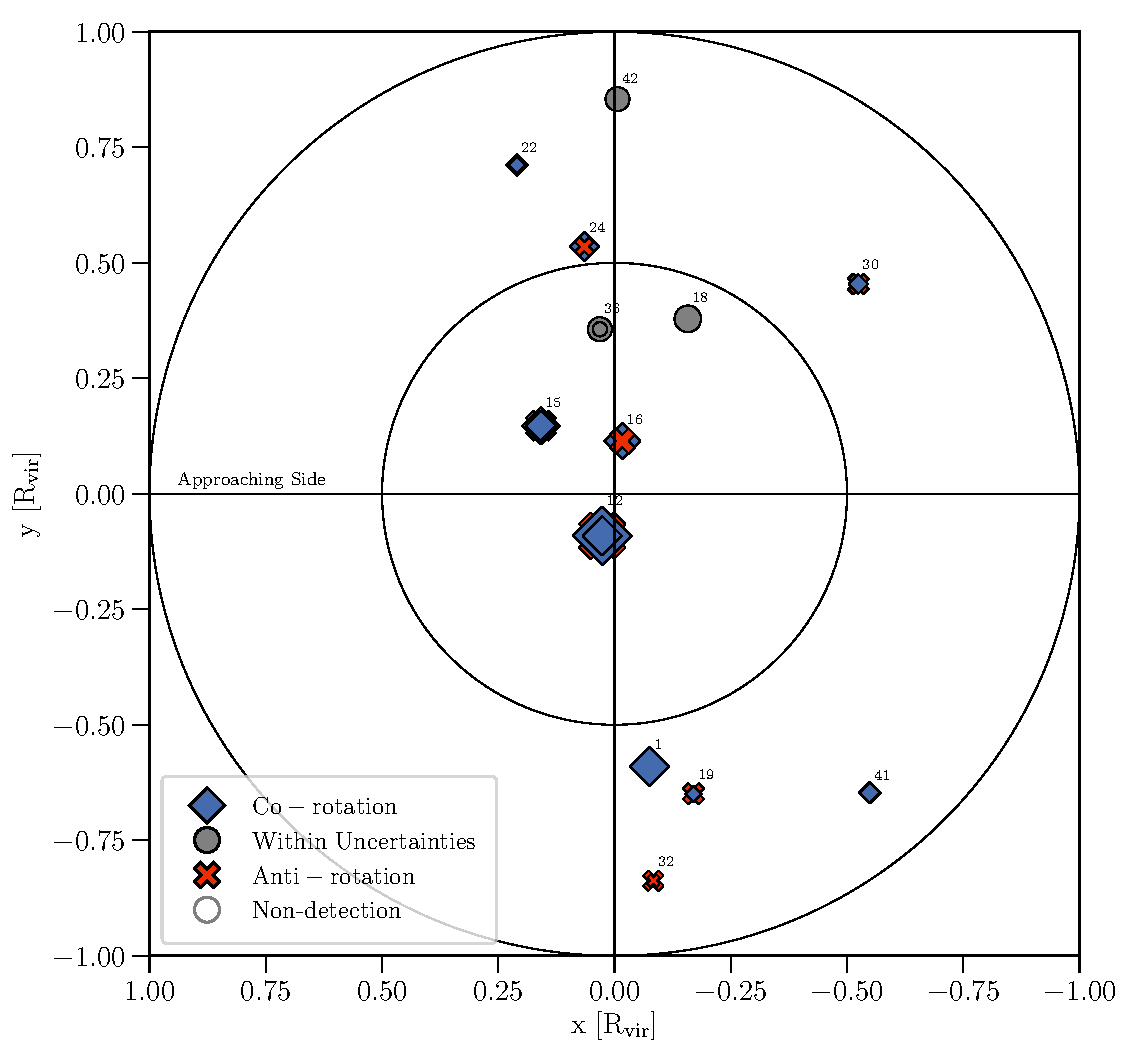
\includegraphics[width=0.82\linewidth]{Chap4/figures/SALTmap_velstrict_False_non_True_Lstar_0-100_minsep_False_zoom_1_inclim_0.pdf}}
  \caption{\small{A map of the locations of each absorber normalized with respect to the galaxy virial radius. A zoom in showing only those systems within $1 R_{\rm vir}$ (exactly the same as Figure \ref{full_map} within $1 R_{\rm vir}$). The color and style of each point indicates the line-of-sight velocity compared to that of the rotation of the nearby galaxy. Blue diamonds indicate co-rotation, red crosses indicate anti-rotation, and grey circles indicate cases where either is possible due to a combination of orientation and velocity uncertainties. The size of each point is scaled to reflect the EW of the absorber. All galaxies are rotated to PA = 90 or 270, such that their major axis' are horizontal and their approaching side is on the left as indicated. The number identifiers correspond to the system number given in column (1) of Table \ref{model}.}}
\vspace{0pt}
\label{zoom_map}
\end{figure}


A cursory look at Figures \ref{full_map} and \ref{zoom_map} reveals several interesting results. First, the highest EW absorbers are all found within $1 R_{\rm vir}$. This is not surprising, given the results by numerous groups claiming an impact parameter - equivalent width anti-correlation (see e.g., \citealt{french2017}, and references therein). Second, many of our absorbers, and many co-rotating ones, lie in the $1 - 2 R_{\rm vir}$ region. Previously, most groups have concentrated on studying the sub-$1 R_{\rm vir}$ regime, but doing so clearly does not reveal the whole physical picture. Third, most ($52\%$) of galaxy-QSO systems reveal multiple distinct velocity components, and they tend to be oriented such that one component is co- and one anti-rotating with the nearby galaxy.

However, a more in-depth look at the underlying data reveals that many of these absorbers have $\Delta v$ much larger than the inclination-corrected galaxy rotation velocity ($v_{\rm rot}$). In other words, the velocity of the absorber relative to galaxy systemic if much greater than the rotation velocity of the galaxy disk. This results in a much smaller fraction of co-rotating absorbers when compared to our cylindrical and NFW profile models (39\% and 43\%, respectively), which will never output a velocity higher than $v_{\rm rot}$. In undertaking this study we necessarily must begin by assuming that absorption within some velocity limit and impact parameter from a galaxy is likely associated with that galaxy. To start with we set these limits at $\Delta v_{\rm max} = 400$ \kms~and $\rho_{\rm max} = 3 R_{\rm vir}$. 

Let us now instead consider only absorbers with $\Delta v \leq v_{\rm rot} \pm 10$ \kms, or absorbers with velocities differences no greater than the maximal galaxy rotation velocity (including a $\pm$10 \kms~buffer to account for velocity and linewidth uncertainties; in other words the we are only considering absorbers where $|v_{\rm Ly\alpha} - v_{\rm sys}| \leq v_{\rm rot}~\pm 10$ \kms~, which are those absorbers within the velocity range of $\pm$ rotation $-$ this constraint removes 22 from our original sample of 65 absorbers). This constraint thus focuses only on absorbers whose velocity falls within the range of possible rotation-related velocities. While this could be interpreted as a bias in the sample, we are really only setting the $\Delta v$ velocity separation limit on a case-by case basis instead of globally given the additional information available to us. We could just as easily have started this study by looking for only absorbers within $\Delta v = 150$ \kms~of a galaxy instead of $\Delta v = 400$ \kms, which would have a similar overall effect. This criteria instead narrows the focus to only those absorbers kinematically close enough to a galaxy to test for a co-rotation fraction with minimal contamination from $\rm Ly\alpha$ forest lines.

\begin{figure}[ht!]
\centering
  \subfigure[]{\includegraphics[width=0.78\linewidth]{Chap4/figures/SALTmap_NFW_model_velstrict_True_non_True_Lstar_0-100_minsep_False_inclim_0.pdf}}
  \caption{\small{A map of the locations of each absorber normalized with respect to the galaxy virial radius. The color and style of each point indicates the NFW rotation model results for each absorber with a $v_{\rm Ly\alpha} \leq v_{\rm rot}$ constraint imposed. Concentric rings indicate distances of 1, 2, and 3 $R_{vir}$. Blue diamonds indicate co-rotation, red crosses indicate anti-rotation, and grey circles indicate cases where either is possible due to a combination of orientation and velocity uncertainties. The size of each point is scaled to reflect the EW of the absorber. All galaxies are rotated to PA = 90 or 270, such that their major axis' are horizontal and their approaching side is on the left as indicated. The number identifiers correspond to the system number given in column (1) of Table \ref{model}.}}
%\vspace{5pt}
\label{nfw_map}
\end{figure}


With this rotation-based velocity constraint in place the co-rotating fractions for our cylindrical and NFW models increase to 58\% and 63\%, while the apparent co-rotation fraction decreases slightly to 50\%. Consistently, we find our cylindrical model to predict an $\sim 8-10 \%$ higher co-rotation fraction than the straight apparent velocity analysis yields, and our NFW model tends to predict an additional $\sim 5\%$ increase. This is a not wholly unexpected, and yet refreshing result; simulations have predicted that galaxies are strongly linked to their surroundings and share angular momentum, which should result in a higher than $50\%$ halo-gas co-rotation fraction. However, the simple apparent on-sky velocity method ignores the complexities of sampling a 3-dimensional structure with a 1-dimensional QSO sightline. It appears then that the NFW model, the most physically motivated of the three, systematically recovers a higher fraction of this co-rotating gas. For brevity's sake we will concentrate only on the NFW model results from here onwards. Figure \ref{nfw_map} shows another absorber location map, this time colored according to our NFW model results.


One additional constraining step we consider is to only include galaxies which have no neighbors within at least 20 kpc. The disruptions caused by near neighbors to both galaxy \HI~disks and halos has been well established observationally, so a 20 kpc minimum separation should at least remove the systems most likely to be disrupted. This constraint alone leads to a co-rotating fraction of 50\%. Combining both constraints results in a 62\% co-rotating fraction.

%\footnote{From here on we concentrate on the results using our NFW profile model. The cylindrical model results do not differ in a systematically interesting way.}


%\begin{figure}[ht!]
%        \centering
%        \vspace{0pt}
%        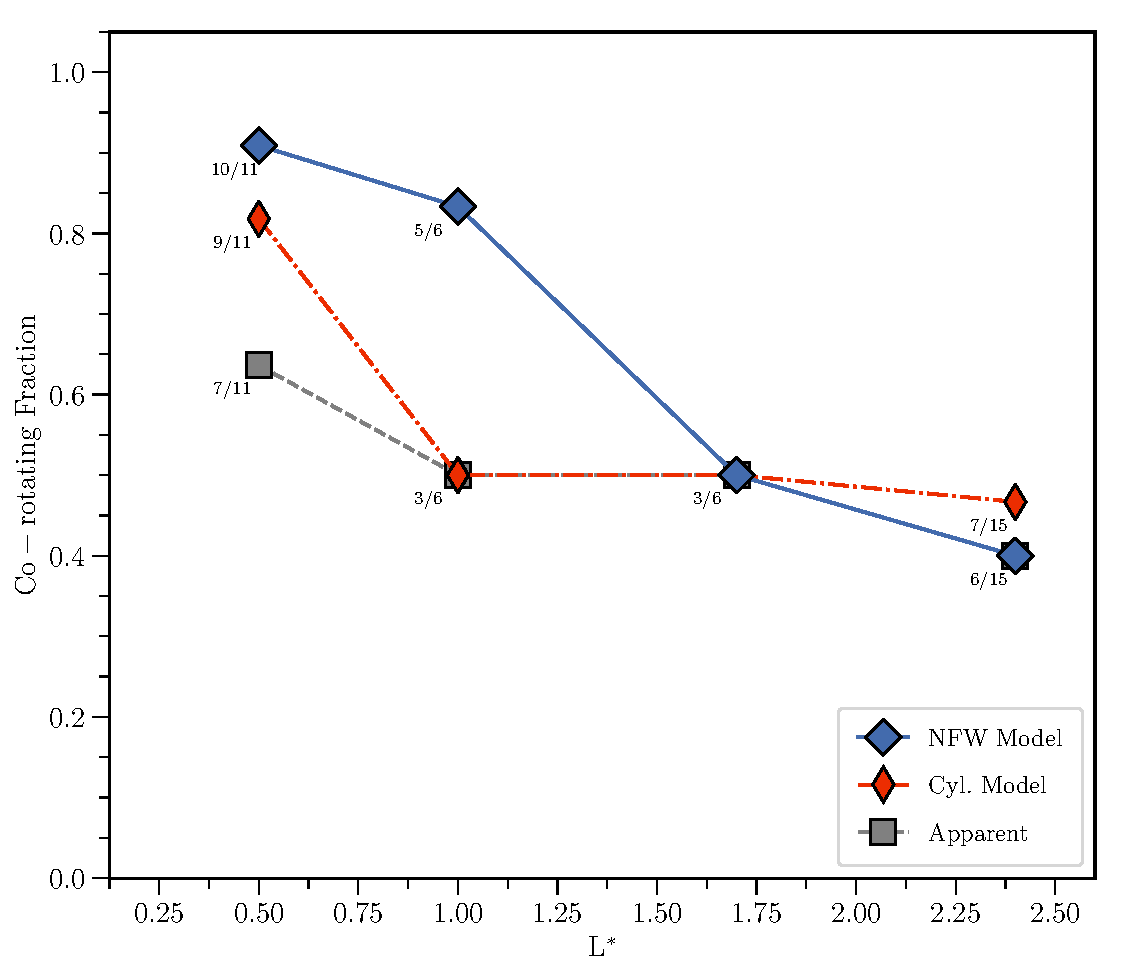
\includegraphics[width=0.49\textwidth]{SALT_corotate_vs_Lstar_velstrict_True_non_True_Lstar_05_minsep_False_ALLmodel.pdf}
%        \caption{\small{The fraction of co-rotating absorbers as a function of \Lstar. The upper edges of the \Lstar bins are located at 0.5, 1.0, 1.7, and $>1.7$\Lstar (i.e., all systems $1.7$\Lstar and higher). }}
%%        \vspace{-5pt}
%        \label{Lstar_fraction}
%\end{figure}
%\begin{figure}[ht!]
%        \centering
%        \vspace{0pt}
%        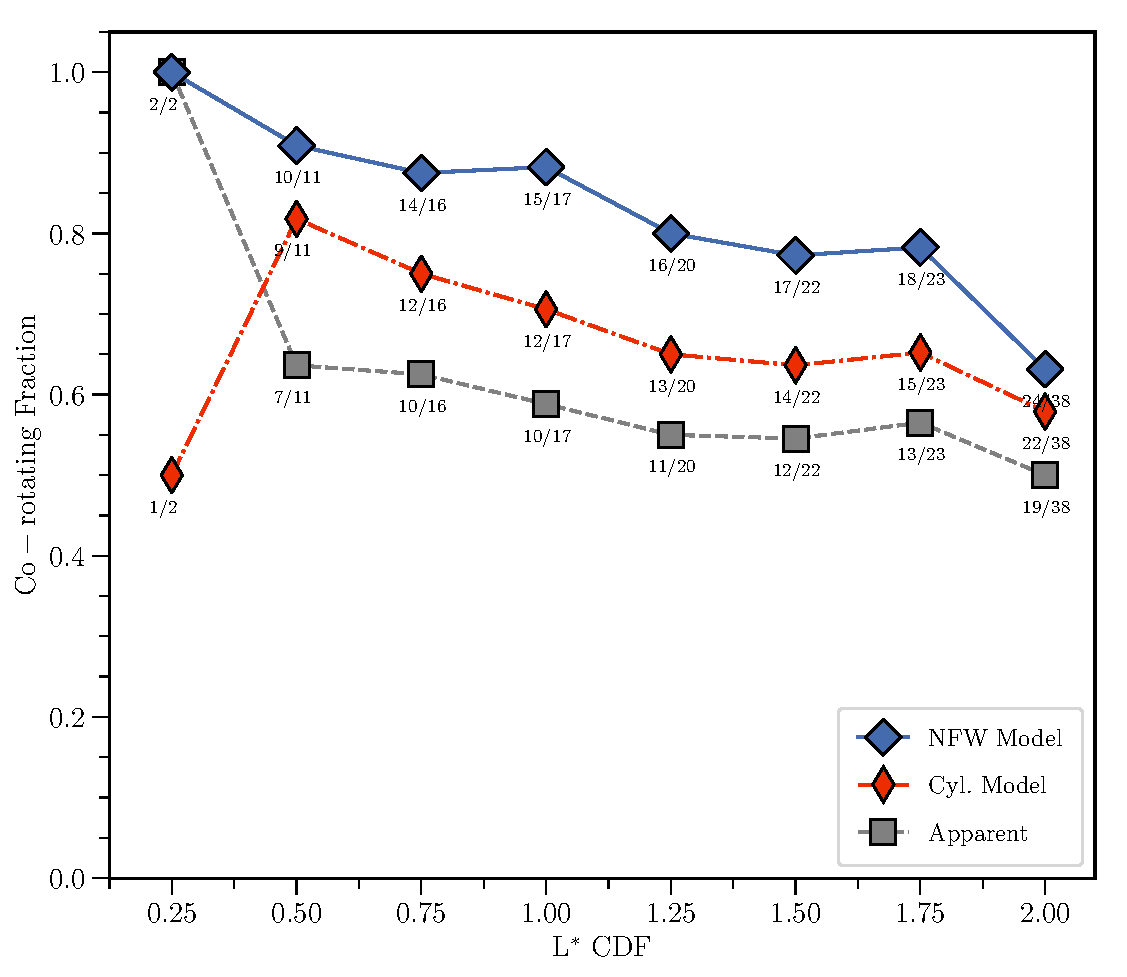
\includegraphics[width=0.49\textwidth]{SALT_corotate_vs_Lstar_minimum_velstrict_True_non_True_Lstar_05_minsep_False_ALLmodel.pdf}
%        \caption{\small{The fraction of co-rotating absorbers as a function of cumulative $L^{*}$ distribution. All systems are included at $L^{*}$=1.6 (this bin includes galaxies brighter than 1.6\Lstar as well), then only galaxies with \Lstar$ \leq 1.4$ are included at \Lstar =1.4, and so on.}}
%%        \vspace{-5pt}
%        \label{Lstar_fraction_cdf}
%\end{figure}


\subsection{Co-rotation as a function of \Lstar}
Next, we consider the effect of galaxy luminosity. We separate our sample around $0.6$\Lstar,  while keeping our $\Delta v \leq v_{\rm rot} \pm 10$ \kms~constraint and relaxing the 20 kpc nearest-neighbor criteria in order to maximize the sample size. This results in 13 absorbers near $L \leq 0.6$\Lstar~galaxies and 30 around more luminous galaxies. The co-rotating fraction around luminous galaxies is then 48\%, compared to 92\% around $L \leq 0.6$\Lstar~ galaxies. Figure \ref{nfw_lstar_map} shows an absorber map for these $L \leq 0.6$\Lstar~ galaxies only. In fact, the co-rotating absorber fraction smoothly decreases as a function of \Lstar, as shown in Figure \ref{Lstar_fraction}(a). In this figure we have binned galaxy-absorber systems into the following 4 ranges: $[0-0.5],~(0.5-1.0],~(1.0-1.7],$ and $(1.7-\infty)$. This uneven bin spacing was chosen to produce as evenly occupied bins as possible, and does not affect the overall trend. Unfortunately there are a large number of systems between $1.7-1.8$ \Lstar, so no splitting exists to produce perfectly even bins. The co-rotation fraction is labeled explicitly underneath each data point for clarity.

In Figure \ref{Lstar_fraction_cdf} we consider the co-rotation fraction as a function of the cumulative \Lstar~ distribution (i.e., every consecutive \Lstar~ bin includes all previous bins' data as well). Here, bins are evenly distributed in $0.25$\Lstar~ increments with the final bin containing all systems. Thus, nearly $90\%$ of absorbers near \Lstar~ or fainter galaxies are co-rotating based on our NFW model results, but this fraction decreases to $\sim 80\%$ for $1.5$\Lstar~ or fainter galaxies, and to $63\%$ for all galaxies. As seen in Figure \ref{Lstar_fraction_cdf}, this trend is also model independent; it appears nearly identically but offset downward in both the cylindrical model (red-rhombus) and apparent velocity only (grey-square) samples.

%As seen in red rhombus and grey square markers in Figure \ref{Lstar_fraction_cdf}, this trend appears identically but offset downward in both the cylindrical model and apparent velocity only samples.


\begin{figure}
\centering
  \subfigure[]{\includegraphics[width=0.55\linewidth]{Chap4/figures/SALT_corotate_vs_Lstar_velstrict_True_non_True_Lstar_06_minsep_False_ALLmodel.pdf}}\label{Lstar_fraction}
  
  \subfigure[]{\includegraphics[width=0.55\linewidth]{Chap4/figures/SALT_corotate_vs_Lstar_minimum_velstrict_True_non_True_Lstar_06_minsep_False_ALLmodel.pdf}\label{Lstar_fraction_cdf}}
  \caption{\small{\textbf{Top:} The fraction of co-rotating absorbers as a function of \Lstar. The upper edges of the \Lstar~ bins are located at 0.5, 1.0, 1.7, and $>1.7$ \Lstar~ (i.e., all systems $1.7 $\Lstar~ and higher). \textbf{Bottom:} The fraction of co-rotating absorbers as a function of cumulative \Lstar~ distribution. All systems are included at the \Lstar$=2.0$ bin (this bin includes galaxies brighter than 2.0\Lstar~ as well), then only galaxies with \Lstar~ $ \leq 1.8$ are included at \Lstar~$ =1.8$, and so on.}}
\vspace{0pt}
\label{Lstar_fraction}
\end{figure}



\begin{deluxetable}{l | c c c | c c | c c}
\tabletypesize{\footnotesize}
\rotate
\tablewidth{0pt}
\tablecaption{CGM Rotation: Summary of Results\label{results}}
\tablehead{
\colhead{Sub-sample}  		&  \colhead{Co-rotating} 		&  \colhead{Anti-rotating}		&  \colhead{Uncertain}  	&  \colhead{Co-rotating} 		&  \colhead{Anti-rotating} 		&  \colhead{Co-rotating} 		&  \colhead{Anti-rotating}	\\
			  			&          			 		& 			 			&					& $\rho \leq 1$				& $\rho \leq 1$				& $\rho >$ 1				& $\rho > 1$		}
\startdata
Apparent Vel.				&	30					&	26					&	9				&		13				&		9				&	17					&	17				\\
\hline
Cyl. Model				&	22					&	34					&	9				&		9				&		13				&	13					&	21				\\
\hline
NFW Model				&	24					&	32					&	9				&		9				&		13				&	15					&	19				\\
\hline \\
\hline
NFW w/ Constraint:			&	24					&	14					&	5				&		9				&		6				&	15					&	8				\\
$\Delta v \leq \lvert v_{\rm rot} \rvert \pm 10$ \kms		&						&						&					&						&						&						&					\\
\hline
NFW w/ Constraint:			&	13					&	13					&	6				&		3				&		3				&	10					&	10				\\
Nearest $\rho \geq 20$ kpc	&						&						&					&						&						&						&					\\
\hline
NFW w/ Both Constraints		&	13					&	8					&	2				&		3				&		1				&	10					&	7				\\
\hline \\
\hline
NFW w/ $\Delta v$ Constraint:	&	12					&	1					&	0				&		5				&		1				&	7					&	0				\\
$[0 \leq $\Lstar $ \leq 0.6]$		&						&						&					&						&						&						&					\\
\hline
NFW w/ $\Delta v$ Constraint:	&	12					&	13					&	5				&		4				&		5				&	8					&	8				\\
$[$\Lstar $ > 0.6]$				&						&						&					&						&						&						&					\\
\enddata
\tablecomments{Comments.}
%\vspace{-5pt}
\end{deluxetable}

Given recent simulation results suggesting that co-rotating accretion gas is predominately cold-mode for low-mass galaxies in the local Universe, this may be a signature of this co-rotating, cold-mode accreting gas. Additionally, \cite{lutz2018} find that galaxies with high \HI mass compared to their stellar mass have higher halo angular momentum, which may be impeding their ability to efficiently form stars. While we do not have independent measures of \HI and stellar mass for our galaxies, it may not be unreasonable to think that these high angular momentum galaxies reside toward the lower luminosity end of our sample.

\begin{figure}[ht!]
        \centering
        \vspace{0pt}
        \includegraphics[width=0.85\textwidth]{Chap4/figures/SALTmap_NFW_model_velstrict_True_non_True_Lstar_0-06_minsep_False_inclim_0.pdf}
        \caption{\small{A map of the locations of each absorber normalized with respect to the galaxy virial radius. The color and style of each point indicates the NFW rotation model results for each absorber with $\Delta v \leq v_{rot}$ and \Lstar $\leq 0.6$ constraints imposed. Blue diamonds indicate co-rotation, red crosses indicate anti-rotation, and grey circles indicate cases where either is possible due to a combination of orientation and velocity uncertainties. The size of each point is scaled to reflect the EW of the absorber. Concentric rings indicate distances of 1, 2, and 3 $R_{vir}$. All galaxies are rotated to PA = 90 or 270, such that their major axis' are horizontal and their approaching side is on the left as indicated. The number identifiers correspond to the system number given in column (1) of Table \ref{model}.}}
        \vspace{5pt}
        \label{nfw_lstar_map}
\end{figure}

\begin{figure}
\centering
  \subfigure[]{\includegraphics[width=0.49\linewidth]{Chap4/figures/SALT_bhist_NFW_velstrict_True_non_True_Lstar_06_minsep_False_fits_True.pdf}\label{b_hist}}
  \subfigure[]{\includegraphics[width=0.5\linewidth]{Chap4/figures/SALT_b_vs_dv_NFW_velstrict_True_non_True_Lstar_False_minsep_False_fits_True.pdf}}\label{b_vs_dv2}
  \caption{\small{\textbf{Top:} The distributions of Doppler $b$-parameters for all Ly$\alpha$ absorbers with $\Delta v \leq v_{\rm rot} \pm 10$ \kms. The co-rotating versus anti-rotating designation here is based on NFW results. In the middle we do the same but only for $\rho \leq 1 R_{vir}$, and on the bottom we separate based on absorbers near \Lstar $\leq 0.6$ (blue) and \Lstar $ > 0.6$ (red-hatched) galaxies.  \textbf{Bottom:} The Doppler $b$-parameters of each absorber as a function of $\Delta v$, split into co-rotating (blue diamonds) and anti-rotating (red crosses). The data point for the NGC3067-3C232 LLS ($b = 245.2 \pm 25.9,  ~\Delta v = -68.0 \pm 11$ \kms, co-rotating) is not shown in order to highlight the majority distribution in greater detail.}}
\vspace{5pt}
\label{b_vs_dv2}
\end{figure}


\subsection{Doppler $b$-parameters}
Finally, we consider the Doppler $b$-parameters of our absorber sample. Figure \ref{b_hist} shows the distribution of $b$-parameters for all velocity-constrained Ly$\alpha$ absorbers ($\Delta v \leq v_{\rm rot} \pm 10$ \kms). In the top panel of Figure \ref{b_hist} we separate them into co-rotating and anti-rotating subsets, in the middle panel we do the same but only for $\rho \leq 1 R_{\rm vir}$, and on the bottom we separate based on absorbers near \Lstar $\leq 0.6$ and \Lstar $ > 0.6$ galaxies. Interestingly, we find that \emph{lower} $b$-parameter absorbers tend to be both anti-rotating and found near \Lstar $> 0.6$ galaxies. As we've previously discussed however, the picture described by the simulations of \cite{stewart2011b} and others describes a scenario where co-rotating gas is predominately the product of cold-mode accretion. Hotter, outflowing gas would likely carry angular momentum from the disk with it, but this would be quickly lost as the outflows expand into the halo and result in negligible observable rotation. 

In Figure \ref{b_vs_dv2}(b) we show how the $b$-parameters vary as a function of $\Delta v$ for co-rotating versus anti-rotating absorbers. We would expect the co-rotating sample to occupy a narrower $\Delta v$ space based on their definition ($\Delta v$ fitting within the velocity bounds given by our NFW model), but the elevated $b$-parameters for these compared to the relatively flat distribution for anti-rotators is intriguing. Aside from a single $\rm Ly\alpha$ line toward SDSSJ104335.90+115129.0 and NGC3351, all the anti-rotators have $b \lesssim 50$ \kms. As these are higher than expected for purely thermal motions within a single $\rm Ly\alpha$ structure, we may be observing either a number of clouds that are close in velocity space or a filament with a range of turbulent, internal velocities. In this scenario these high $b$-parameters would be consistent with filamentary inflows versus around higher \Lstar~ galaxies where virial shocks are perhaps breaking larger structures into smaller, more isolated cloudlets and producing lower $b$-parameter absorption.

%\textbf{MORE}

%Could some of this double red/blue separated sets be infall?


%\begin{figure}[h]
%        \centering
%        \vspace{0pt}
%        \includegraphics[width=0.49\textwidth]{Chap4/figures/SALT_b_vs_dv_NFW_velstrict_True_non_True_Lstar_False_minsep_False_fits_True.pdf}
%        \caption{\small{The Doppler b-parameters of each absorber as a function of $\Delta v$, split into co-rotating (blue diamonds) and anti-rotating (red crosses). The data point for the NGC3067-3C232 LLS ($b = 245.2 \pm 25.9,  ~\Delta v = -68.0 \pm 11$ \kms) is not shown in order to highlight the majority distribution in greater detail. The co-rotating versus anti-rotating designation here is based on NFW results.}}
%%        \vspace{-5pt}
%        \label{b_vs_dv}
%\end{figure}
%\begin{figure}[h]
%        \centering
%        \vspace{0pt}
%        \includegraphics[width=0.45\textwidth]{Chap4/figures/SALT_bhist_NFW_velstrict_True_non_True_Lstar_06_minsep_False_fits_True.pdf}
%        \caption{\small{Histograms showing the distributions of Doppler b-parameters for all Ly$\alpha$ absorbers with $v_{Ly\alpha} \leq v_{rot} \pm 10$ \kms. In the top panel we separate them into co-rotating (blue) and anti-rotating (red-hatched) subsets based on our NFW model results, in the middle we do the same but only for $\rho \leq 1 R_{vir}$, and on the bottom we separate based on absorbers near $L^{*} \leq 0.5$ (blue) and $L^{*} > 0.5$ (red-hatched) galaxies. The co-rotating versus anti-rotating designation here is based on NFW results.}}
%%        \vspace{-5pt}
%        \label{b_hist}
%\end{figure}




%\begin{figure}[t!]
%\centering
%  \subfigure[]{\includegraphics[width=0.87\linewidth]{Chap4/figures/fig2.pdf}}{\label{line}}
%  \subfigure[]{\includegraphics[width=1.\linewidth]{Chap4/figures/fig3.pdf}\label{impactmap}}
%  \caption{\small{a) An example of 2 Ly$\alpha$ lines found in the Mrk290 sightline at 3090 and 3192 . b) A map of \textit{all} galaxies within a 500 kpc impact parameter of target Mrk290 sightline and with velocity ($cz$) within 400 $\rm km\, s^{-1}$ of absorption detected at 3192 $\rm km\, s^{-1}$ (central black star). The galaxy NGC5987 ($v=3010$ $\rm km\, s^{-1}$, inclination = $65^{\circ}$) can be unambiguously paired with the Ly$\alpha$ absorption features at $v=3090, 3192$ $\rm km\, s^{-1}$ because it is the largest and closest galaxy in both physical and velocity space to the absorption feature.}}
%\vspace{5pt}
%\end{figure}


\section{Summary} \label{summary}
We have presented complimentary COS Ly$\alpha$ absorption-line and nearby galaxy rotation curve analysis for a sample of 42 galaxy-QSO pairs, resulting in the largest yet sample of its kind. Our main conclusions are the following:
\vspace{10pt}

1. The fraction of Ly$\alpha$ absorbers appearing to co-rotate with the nearby galaxy smoothly declines as a function galaxy luminosity (\Lstar). Our overall co-rotation fraction is consistent with the simulation results of \cite{stewart2011b, stewart2013}, and effect of galaxy luminosity on halo gas co-rotation is consistent with predicted cold-mode filamentary accretion schemes. 

\vspace{10pt}

%The fraction of co-rotating $\rm Ly\alpha$ absorbers smoothly decreases as a function of the luminosity (\Lstar) of the nearby (probable-) host galaxy. 
2. Based on our NFW halo model, 92\% of absorbers co-rotate around $\rm \leq 0.6 $\Lstar~ galaxies, which falls to 77\% around $\rm \leq 1.5$ \Lstar~ galaxies, and down to 63\% around all galaxies at $z \sim 0$.

\vspace{10pt}

3. Two thirds of all $\rm Ly\alpha$ absorbers are found with velocity separations less than or equal to the nearby galaxy rotation velocity ($\Delta v \leq \lvert v_{\rm rot} \rvert \pm 10$ \kms). This includes systems with multiple galaxies and undoubtedly complex velocity fields. Restricting this study to only isolated galaxy-QSO systems would likely result in an even higher fraction.

%Two thirds of all $\rm Ly\alpha$ absorbers within $3 R_{\rm vir}$ and $\Delta v = 400$ \kms~of our galaxies with known kinematics reside within $\pm v{\rm rot}$

%A simple cylindrical halo model An NFW rotation curve fit, which results in a galaxy rotation velocity which approaches systemic 

\vspace{10pt}

4. A simple cylindrical halo model with rotation velocities smoothly declining based on an NFW rotation curve fit results in the highest co-rotation fraction for $\rm Ly\alpha$ absorbers ($63\%$).

\vspace{10pt}

5. Co-rotating absorbers (when chosen from the sample restricted to $\Delta v \leq \lvert v_{\rm rot} \rvert \pm 10$ \kms) occupy a wide range in Doppler $b$-parameter, while anti-rotators have mostly $b \leq 50$ \kms. A remarkably similar split is found for absorbers near $L \leq 0.6 $\Lstar~ vs $L > 0.6$\Lstar~ galaxies. This could add further evidence for our proposed cold-mode accretion explanation if these enhanced $b$-parameters are caused by the blending of multiple absorption components close in velocity space within a filament.

\vspace{10pt}


\acknowledgements

D. M. F. thanks Claire Murray for useful insights, particularly related to our halo model, and Julie Davis for invaluable SALT data reduction pointers. This research has made use of the NASA/IPAC Extragalactic Database (NED) which is operated by the Jet Propulsion Laboratory, California Institute of Technology, under contract with the National Aeronautics and Space Administration. Based on observations with the NASA/ESA \textit{Hubble Space Telescope}, obtained at the Space Telescope Science Institute (STScI), which is operated by the Association of Universities for Research in Astronomy, Inc., under NASA contract NAS 5-26555. Spectra were retrieved from the Barbara A. Mikulski Archive for Space Telescopes (MAST) at STScI. Some of the observations reported in this paper were obtained with the Southern African Large Telescope (SALT) under program 2016-1-SCI-062 (PI: Wakker). Over the course of this study, D.M.F. and B.P.W. were supported by grant AST-118913 from the National Science Foundation and GO-14240, GO-14268, and GO-14588 from the Space Telescope Science Institute.

%AST-1108913, awarded by the US National Science Foundation, and by NASA grants \textit{HST}-AR-12842.01-A, \textit{HST}-AR-13893.01-A, and \textit{HST}-GO-14240 (STScI). 

%\facility{HST (COS), SALT (RSS)}
\clearpage

%\nocite{*}
%\bibliography{rotation_bib}
%\bibliography{/Users/frenchd/Research/bib}{}
%\bibliography{/Users/clairemurray/Desktop/DMF_thesis/bib}
\bibliography{/Users/frenchd/Research/inclination/git_inclination/thesis/DMF_thesis/bib}
\bibliographystyle{thesis}

\clearpage

\chapappendix

%\section{Galaxy Sample}
%\label{galaxy_sample}

\section{SALT Galaxies} \label{SALT_sample}
In this section we summarize each galaxy-QSO system observed by SALT. We calculate impact parameters to QSOs and galaxy-absorber velocity separations ($\Delta v = v_{\rm Ly\alpha} - v_{\rm sys}$) based on our measured $v_{sys}$ values. Both measured and previously published values for $v_{sys}$ are given in Table \ref{salt_targets} for reference. We provide rotation curves and finder chart images for the sub-sample of galaxies with newly observed SALT data.

\subsection{CGCG039-137}

CGCG039-137 is an isolated Scd type galaxy with a measured systemic velocity $v_{\rm sys} = 6918 \pm 24$ \kms~and inclination of $i = 63^{\circ}$. The QSO RX\_J1121.2+0326 is located nearby at an impact parameter of 99 kpc and azimuth angle of $71^{\circ}$ on the receding side. The data for  RX\_J1121.2+0326 has low signal-to-noise ($\sim 4.2$), but we are able to detect Ly$\alpha$ at 6975 \kms~, which, at $\Delta v = 57$ \kms, lies well within the range of projected velocities consistent with co-rotation (cylindrical model = [-36, 137], NFW = [-37, 164] \kms). 

\begin{figure}[hb]
\centering
  \subfigure[]{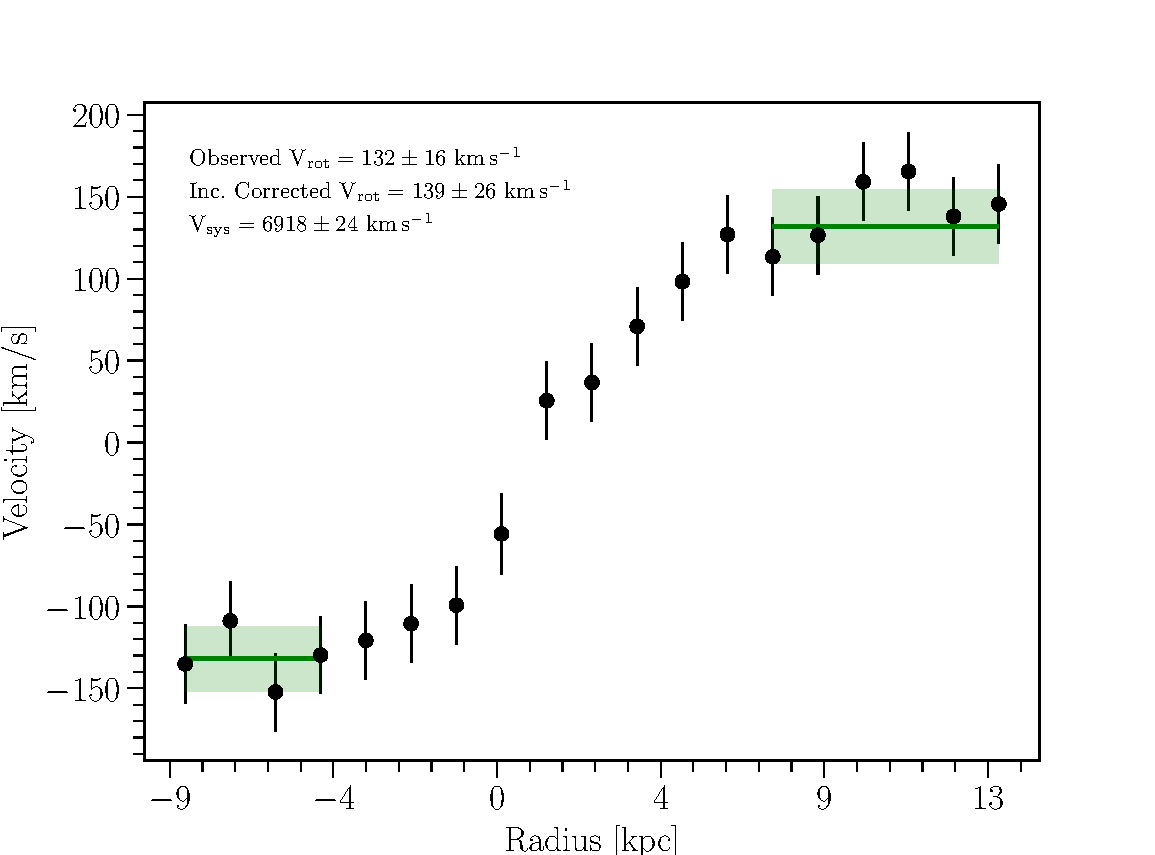
\includegraphics[width=.54\linewidth]{Chap4/figures/CGCG039-137_2_rotation_curve_xphys_helio_vobs_vrotObs_new4.pdf}}{\label{rotationcurve_CGCG039-137}}
  \subfigure[]{\includegraphics[width=0.45\linewidth]{Chap4/figures/CGCG039-137_Finding_chart.jpg}\label{finderchart_CGCG039-137}}
  \caption{\small{a) Rotation curve of CGCG039-137. The solid green line indicates the weighted mean velocity over the corresponding x-axis region, and the shaded green indicates the 1$\sigma$ error in the mean. b) SALT finder chart for CGCG039-137 showing the position of the slit in red.}}
\vspace{0pt}
\end{figure}

%, and SDSSJ112224.10+031802.0 at 491 kpc and $24^{\circ}$ on the approaching side. Ly$\alpha$ absorption is detected in both sightlines within $400$\kms~ of CGCG039-137. 

%The absorber detected toward SDSSJ112224.10+031802.0 occurs at a more distant 6606 \kms ($\Delta v = -312$ \kms). Although this absorber has the correct sign for co-rotation (blue-ward on the approaching side of the disk), the large velocity difference and impact parameter make it unlikely that this absorption can be linked to coherent halo rotation.


\subsection{ESO343-G014}
ESO343-G014 is an edge-on spiral galaxy with a measured systemic velocity $v_{\rm sys} = 9139 \pm$ 32 \kms. It has a smaller neighboring galaxy, 2MASXJ21372816-3824412, located north of it's major axis at a projected distance of 216 kpc and velocity of 9129 \kms. The nearest sightline is towards RBS1768 at $\rho = 466$ kpc and $74^{\circ}$ azimuth angle on the approaching side. We detect 3 blended Ly$\rm \alpha$ absorption components toward RBS1768 at $v_{\rm Ly\alpha} = 9308, 9360, 9434$ \kms~($\Delta v = 169, 221, 295$ \kms). This system is highly blended with galactic S\,{\sc ii}, and therefore their widths are not reliable. All of these are anti-aligned with the rotation of ESO343-G014 relative to the models (cylindrical = [-203, 10], NFW = [-122, 31] \kms). Unfortunately the presence of 2MASXJ21372816-3824412 makes it difficult to attribute this gas solely to ESO343-G014. Additionally, this gas could be attributed to either the approaching or receding side of the disk due to the large impact parameter and high azimuth angle of the sightline.

\begin{figure}[ht]
\centering
  \subfigure[]{\includegraphics[width=.54\linewidth]{Chap4/figures/RFGC3781_2_rotation_curve_xphys_helio_vobs_vrotObs_new4.pdf}}{\label{rotationcurve_ESO343-G014}}
  \subfigure[]{\includegraphics[width=0.45\linewidth]{Chap4/figures/RFGC3781_FindingChart.jpg}\label{finderchart_ESO343-G014}}
  \caption{\small{a) Rotation curve of ESO343-G014. The solid green line indicates the weighted mean velocity over the corresponding x-axis region, and the shaded green indicates the 1$\sigma$ error in the mean. b) SALT finder chart for ESO343-G014 showing the position of the slit in red.}}
\vspace{0pt}
\end{figure}


\subsection{IC5325}
IC5325 is a mostly face-on SAB(rs)bc type galaxy with a measured systemic velocity $v_{\rm sys} = 1512 \pm 8$ \kms. It's inclination is just high enough ($i = 25^{\circ}$) to obtain a reasonable rotation curve. The closest neighboring galaxy is ESO347-G020 to the southeast at 306 kpc and $v_{sys} = 1745$ \kms. Three other much smaller galaxies are also located $\sim 450$ kpc to the southwest. The background QSO RBS2000 is located northeast at $\rho = 314$ kpc and  $64^{\circ}$ azimuth angle on the approaching side of IC5325. We detect Ly$\alpha$ at $v_{\rm Ly\alpha} = 1598$ \kms~($\Delta v = 86$ \kms) towards RBS2000. While this velocity is anti-aligned with the rotation the disk gas relative to our model predictions (cylindrical = [-41, -20], NFW = [-29, 1] \kms), the low inclination angle of IC5325 leads to a highly uncertain position angle. Without additional observations, we cannot say for certain if the location of RBS2000 actually lies on the approaching or receding side. This position angle uncertainty also means our SALT rotation curve is a lower limit on the true rotation velocity of IC5325.

\begin{figure}[ht]
\centering
  \subfigure[]{\includegraphics[width=.54\linewidth]{Chap4/figures/IC5325_2_rotation_curve_xphys_helio_vobs_vrotObs_new4.pdf}}{\label{rotationcurve_IC5325}}
  \subfigure[]{\includegraphics[width=0.45\linewidth]{Chap4/figures/IC5325_FindingChart.jpg}\label{finderchart_IC5325}}
  \caption{\small{a) Rotation curve of IC5325. The solid green line indicates the weighted mean velocity over the corresponding x-axis region, and the shaded green indicates the 1$\sigma$ error in the mean. b) SALT finder chart for IC5325 showing the position of the slit in red.}}
\vspace{0pt}
\end{figure}


%The velocity of the absorber, $\Delta v = 86$\kms, is also outside the range of projected co-rotation velocities

% Two galaxies are neighboring IC5325 to the South and East: PGC071660 at XXX kpc and NGC7552 at XXX kpc. 


\subsection{MCG-03-58-009}
MCG-03-58-009 is a massive and very isolated Sc type galaxy at a measured systemic velocity of $v_{\rm sys} = 9015 \pm 19$ \kms~and inclination angle of $i = 49^{\circ}$. The background QSO MRC2251-178 is located southeast at $\rho = 355$ kpc at an azimuth angle of $71^{\circ}$ on the receding side. We detect a weak Ly$\rm \alpha$ absorber at $v_{\rm Ly\alpha} = 9029$ \kms~($\Delta v = 14$ \kms) towards MRC2251-178. This absorber velocity falls well within the expected range for co-rotation relative to our models (cylindrical = [-26, 137], NFW = [-42, 83] \kms). Although this absorber matches the velocity expected for co-rotation, the velocity difference ($\Delta v = 14$ \kms) is also within the systemic velocity uncertainty for MCG-03-58-009. The relative weakness of this absorber (EW = $62 \pm 4$ m\AA) is somewhat unusual given it's proximity (just outside of 1 $R_{vir}$) to a massive galaxy. If this is representative of an isolated system such as MCG-03-58-009, then we should expect the halo rotational velocity to approach systemic by 1 $R_{vir}$.

\begin{figure}[ht]
\centering
  \subfigure[]{\includegraphics[width=.54\linewidth]{Chap4/figures/MCG-03-58-009_2_rotation_curve_xphys_helio_vobs_vrotObs_new4.pdf}}{\label{rotationcurve_MCG-03-58-009}}
  \subfigure[]{\includegraphics[width=0.45\linewidth]{Chap4/figures/MCG-03-58-009_FindingChart.jpg}\label{finderchart_MCG-03-58-009}}
  \caption{\small{a) Rotation curve of MCG-03-58-009. The solid green line indicates the weighted mean velocity over the corresponding x-axis region, and the shaded green indicates the 1$\sigma$ error in the mean. b) SALT finder chart for MCG-03-58-009 showing the position of the slit in red.}}
\vspace{0pt}
\end{figure}



\subsection{NGC1566}
NGC1566 is a SAB(rs)bc type galaxy with measured systemic velocity of $v_{\rm sys} = 1502 \pm 15$ \kms~and inclination angle of $i = 46^{\circ}$. There are several other large galaxies at $\rho \gtrsim 200$ kpc from NGC1566 (e.g., NGC1549, NGC1596, and NGC1581). The closest QSO sightline is toward HE0429-5343, northeast of NGC1566 at $\rho = 256$ kpc and $60^{\circ}$ azimuth angle. We detect Ly$\rm \alpha$ absorption toward HE0429-5343 at $v_{\rm Ly\alpha} = 1167, 1358$ \kms~($\Delta v = -335, -144$ \kms). Both of these absorbers have the correct velocity \emph{sign}, but we would expect a smaller velocity for co-rotation based on our model results (cylindrical = [-53, -2], NFW = [-22, 17] \kms). Unfortunately NGC1617 is slightly closer to this sightline than NGC1566, at $\rho = 233$ kpc and $v_{\rm sys} = 1063$ \kms, so it is not possible to confidently attribute these absorbers to NGC1566.

A more distant QSO sightline toward 1H0419-577 is located to the south at $\rho = 303$ kpc and just east of the receding side of the major axis at an azimuth angle of $10^{\circ}$. We detect Ly$\rm \alpha$ at $v_{\rm Ly\alpha} = 1123, 1188, 1264$ \kms~($\Delta v = -379, -314, -238$ \kms), all of which are the wrong sign for co-rotation relative to our models (cylindrical = [48, 76], NFW = [-2, 31] \kms). This sightline is \emph{also} actually closer to a small group of galaxies including NGC1549, NGC1546 and NGC1536, all with systemic velocities near $\sim 1200$ \kms. Additionally, this absorber system contains C\,{\sc iii}, C\,{\sc iv}, Si\,{\sc ii}, Si\,{\sc iii}, Si\,{\sc iv} lines. These lines likely are associated with this group rather than with NGC1566. 

\begin{figure}[ht]
\centering
  \subfigure[]{\includegraphics[width=.54\linewidth]{Chap4/figures/NGC1566_2_rotation_curve_xphys_helio_vobs_vrotObs_new4.pdf}}{\label{rotationcurve_NGC1566}}
  \subfigure[]{\includegraphics[width=0.45\linewidth]{Chap4/figures/NGC1566_FindingChart.jpg}\label{finderchart_NGC1566}}
  \caption{\small{a) Rotation curve of NGC1566. The solid green line indicates the weighted mean velocity over the corresponding x-axis region, and the shaded green indicates the 1$\sigma$ error in the mean. b) SALT finder chart for NGC1566 showing the position of the slit in red.}}
\vspace{0pt}
\end{figure}

%(approximately $\Delta v \sim \pm40$ \kms~projected).

%NGC1566 is well sampled (5 nearby QSO sightlines), but unfortunately also part of a complex environment of neighboring galaxies. 

%We detect Ly$\alpha$ in all 5 of these sightlines. The farthest three, HE0439-5254, RBS567, and HE0435-5304, are clustered close together toward the northeast of NGC1566 at 459, 423, and 396 kpc and $\sim 60^{\circ}$ azimuth angle. HE0439-5254 and RBS567 are both located beyond our 2 x 3 $R_{vir}$ model limits and therefore are only included here for the sake of completeness. The slightly closer HE0435-5304 sneaks under the limit.

%HE0429-5343 is in the same direction and azimuth angle but closer at $\rho = 256$ kpc, and shows Ly$\alpha$ absorption at 1167 and 1358 \kms. These absorbers both have the correct velocity \emph{sign}, but we would expect a smaller velocity for co-rotation (approximately $\Delta v \sim \pm40$ \kms~projected). This difference could be explained by invoking either a warped extended disk, or perhaps inflowing gas.



\subsection{NGC3513}
NGC3513 a mostly face-on SB(rs)c galaxy with measured systemic velocity $v_{\rm sys} = 1204 \pm 12$ \kms. It has a companion galaxy in NGC3511 at $\rho = 44$ kpc and $v_{\rm sys} = 1109$ \kms~(NGC3513 diameter $D = 22.1$ kpc, NGC3511 diameter $D = 28.1$ kpc). The background QSO H1101-232 is located directly south of the pair at $\rho = 60$ kpc and azimuth angle of $67^{\circ}$ on the receding side. We detect Ly$\rm \alpha$ at $v_{\rm Ly\alpha} = 1182$ \kms~($\Delta v = -22$ \kms) toward H1101-232. NGC3513 appears to be rotating slowly, with a maximal inclination-corrected rotation velocity of $v_{\rm rot} / \sin(\emph{i}) = 22 \pm 24$ \kms. The $\Delta v = -22$ \kms~for this absorber is opposite in sign for co-rotation on the sky and just outside our predicted model velocity range (cylindrical = [-19, 27], NFW = [-19, 28] \kms). Given that NGC3511 is so close, this absorber's velocity is probably subject to a complex velocity field influenced by both NGC3511 and NGC3513. For this reason we have marked this galaxy as ``uncertain" in all map plots and have not included it in our statistical results. This absorber system also contains C\,{\sc iv}, N\,{\sc v}, Si\,{\sc ii}, Si\,{\sc iii}, and Si\,{\sc iv} lines.

\begin{figure}[hb]
\centering
  \subfigure[]{\includegraphics[width=.54\linewidth]{Chap4/figures/NGC3513_2_rotation_curve_xphys_helio_vobs_vrotObs_new4.pdf}}{\label{rotationcurve_NGC3513}}
  \subfigure[]{\includegraphics[width=0.45\linewidth]{Chap4/figures/NGC3513_Finding_chart.jpg}\label{finderchart_NGC3513}}
  \caption{\small{a) Rotation curve of NGC3513. The solid green line indicates the weighted mean velocity over the corresponding x-axis region, and the shaded green indicates the 1$\sigma$ error in the mean. b) SALT finder chart for NGC3513 showing the position of the slit in red.}}
\vspace{0pt}
\end{figure}



\subsection{NGC3633}
NGC3633 is an isolated, edge-on SAa type galaxy with a measured systemic velocity $v_{\rm sys} = 2587 \pm 7$ \kms. Several locations along the disk of NGC3633 show two velocities for emission. We have combined these into a single velocity measurement via a weighted average. 

The background QSO RX\_J1121.2+0326 is located southeast at $\rho = 184$ kpc and $58^{\circ}$ azimuth on the approaching side of NGC3633. We detect Ly$\rm \alpha$ at $v_{\rm Ly\alpha} = 2605$ \kms~($\Delta v = 18$ \kms) toward RX\_J1121.2+0326. While close to $v_{\rm sys}$, this absorber velocity is just outside our predicted model velocities (cylindrical = [-153, -14], NFW = [-77, 10] \kms). However, this absorber is also very weak and broad, making the velocity center uncertain by at least $\sim 10$ \kms. Taking this along with the uncertainty in $V_{\rm sys}$, this absorber could still be consistent with co-rotation.

\begin{figure}[ht]
\centering
  \subfigure[]{\includegraphics[width=.54\linewidth]{Chap4/figures/NGC3633_2_rotation_curve_xphys_helio_vobs_vrotObs_new4.pdf}}{\label{rotationcurve_NGC3633}}
  \subfigure[]{\includegraphics[width=0.45\linewidth]{Chap4/figures/NGC3633_FindingChart.jpg}\label{finderchart_NGC3633}}
  \caption{\small{a) Rotation curve of NGC4536. The solid green line indicates the weighted mean velocity over the corresponding x-axis region, and the shaded green indicates the 1$\sigma$ error in the mean. b) SALT finder chart for NGC3633 showing the position of the slit in red.}}
\vspace{0pt}
\end{figure}


%There are three nearby sightlines: SDSSJ112005.00+ 041323.0 is straight north at 468 kpc and $78^{\circ}$ azimuth, RX\_J1121.2+0326 is to the southeast at 184 kpc and $58^{\circ}$ azimuth, and SDSSJ112224.10+031802.0 at 413 kpc and $50^{\circ}$ azimuth. 

%Toward RX\_J1121.2+0326 we detect a Ly$\alpha$ absorber at 2605 \kms~on the approaching side, which is essentially systemic velocity for NGC3633. The spectrum of SDSSJ112224.10+031802.0 shows absorbers at 2285 and 2578 \kms, both of which are of the correct sign for co-rotation. We do not detect any Ly$\alpha$ towards the third sightline, SDSSJ112224.10+031802.0.

%SDSSJ112005.00+041323.0 and SDSSJ112224.10+ 031802.0 are both outside of our 2 x 3 $R_{vir}$ model limits. 



\subsection{NGC4536}
NGC4536 is a SAB(rs)bc type galaxy located in the Virgo Cluster at a measured systemic velocity of $v_{sys} = 1867 \pm 33$ \kms~and inclination $i = 61^{\circ}$. The data on the receding side of NGC4536 is quite messy, and may include contamination from background sources. Hence, our measured systemic velocity, and thus rotation velocity of $139 \pm 37$ \kms, have relatively high uncertainty. Other published redshift values available from NED and rotation velocities from the HyperLEDA database are broadly consistent with our values, albeit biased slightly lower and higher in velocity, respectively.

There are 2 sightlines to the southwest of NGC4536, both on the receding side of the galaxy. HE1228+0131 at $ \rho = 338$ kpc and $86^{\circ}$ azimuth has 5 Ly$\rm \alpha$ lines: $v_{\rm Ly\alpha} =$ 1495, 1571, 1686, 1721, 1854 \kms~($\Delta v = -$372, -296, -181, -146, -13 \kms). None of these are of the correct orientation for co-rotation relative to our model predictions (cylindrical = [18, 51], NFW = [2, 32] \kms), and all are more likely to be associated with other nearby galaxies, such as NGC4517A, which is slightly closer to these absorbers in impact parameter and velocity than is NGC4536. At $v_{\rm Ly\alpha}  = 1686$ \kms~we also detect C\,{\sc ii}, C\,{\sc iv}, Si\,{\sc ii}, Si\,{\sc iii}, and Si\,{\sc iv}, and at $v_{\rm Ly\alpha}  = 1721$ \kms~we detect Lyman series from Ly$\rm \alpha$ to Ly$\rm \theta$ as well as C\,{\sc ii}, C\,{\sc iii}, C\,{\sc iv}, Si\,{\sc ii}, Si\,{\sc iii}, and Si\,{\sc iv}.

The second nearby sightline is toward 3C273 at $\rho = 344$ kpc and $46^{\circ}$ azimuth angle, and shows 3 Ly$\rm \alpha$ lines at $v_{\rm Ly\alpha} =$ 1580, 2156, 2267 \kms~($\Delta v = -$287, 289, 400 \kms). Two of these are correctly oriented for co-rotation relative to our model predictions (cylindrical = [87, 121], NFW = [5, 41] \kms), but are too high in velocity to make this scenario probable. Overall, given the number of nearby galaxies and their locations, we would expect these absorbers to trace the overall velocity field instead of the halo rotation of any particular galaxy. After this galaxy was included in the SALT observing queue we realized it is actually located in the Virgo cluster, so we have decided to remove it from the statistical sample in this paper but present the observed data here nonetheless.

\begin{figure}[b]
\centering
  \subfigure[]{\includegraphics[width=.54\linewidth]{Chap4/figures/NGC4536_2_rotation_curve_xphys_helio_vobs_vrotObs_new4.pdf}}{\label{rotationcurve_NGC4536}}
  \subfigure[]{\includegraphics[width=0.45\linewidth]{Chap4/figures/NGC4536_FindingChart.jpg}\label{finderchart_NGC4536}}
  \caption{\small{a) Rotation curve of NGC4536. The solid green line indicates the weighted mean velocity over the corresponding x-axis region, and the shaded green indicates the 1$\sigma$ error in the mean. b) SALT finder chart for NGC4536 showing the position of the slit in red.}}
\vspace{0pt}
\end{figure}


%\textit{Just remove this target entirely? Or leave this discussion in place and not include it in the statistics? In this draft I have removed it entirely from the results.}

%However, the approaching side is well sampled and stable with a value of $v_{rot}=-75pm9$ \kms. For this reason, and assuming symmetry for this grand-design spiral galaxy, we have decided to adopt the same value for the receding side, $v_{rot}=75pm9$ \kms.

% The image of this galaxy is confusing - it looks opposite, because we're 'underneath' it (i.e. the near edge is up, the far edge is away). 


\subsection{NGC4939}
NGC4939 is a large SA(s)bc type galaxy with measured systemic velocity $v_{\rm sys} = 3093 \pm 33$ \kms~and inclination $i = 48^{\circ}$. The background QSO PG1302-102 is located southeast at $\rho = 254$ kpc and $61^{\circ}$ azimuth angle on the approaching side of NGC4939. We detect a Ly$\rm \alpha$ absorber at $v_{\rm Ly\alpha} = 3448$ \kms~($\Delta v = 355$\kms) towards PG1302-102. As this absorber is located on the approaching side, we can easily rule out co-rotation in this case. NGC4939 does not have any close neighbors, so represents an intriguing case against co-rotation for gas past $1 R_{\rm vir}$.

\begin{figure}[ht!]
\centering
  \subfigure[]{\includegraphics[width=.54\linewidth]{Chap4/figures/NGC4939_2_rotation_curve_xphys_helio_vobs_vrotObs_new4.pdf}}{\label{rotationcurve_NGC4939}}
  \subfigure[]{\includegraphics[width=0.45\linewidth]{Chap4/figures/NGC4939_FindingChart.jpg}\label{finderchart_NGC4939}}
  \caption{\small{a) Rotation curve of NGC4939. The solid green line indicates the weighted mean velocity over the corresponding x-axis region, and the shaded green indicates the 1$\sigma$ error in the mean. b) SALT finder chart for NGC4939 showing the position of the slit in red.}}
\vspace{0pt}
\end{figure}


\subsection{NGC5364}
NGC5364 is a SA(rs)bc pec type galaxy at a measured systemic velocity $v_{\rm sys} = 1238 \pm 17$ \kms~and inclination $i = 57^{\circ}$. It is located in a group environment with 5 other large, nearby galaxies. The background QSO SDSSJ135726.27+043541.4 is located southeast at $\rho = 165$ kpc and $84^{\circ}$ azimuth angle on the receding side of NGC5364. We detect Ly$\rm \alpha$ at $v_{\rm Ly\alpha} = 967, 1124$ \kms~($\Delta v = -271, -114$ \kms) toward SDSSJ135726.27+043541.4. These absorbers have the opposite sign for co-rotation relative to our model predictions (cylindrical = [-26, 108], NFW = [-30, 68] \kms). However, because of the orientation of NGC5364 on the sky with respect to this sightline, these absorbers lie extremely close to the inflection point were projected rotation velocities flip to approaching instead of receding. For example, shifting the location of SDSSJ135726.27+043541.4 east by a tenth of a degree ($\sim 20$ kpc) is sufficient to put these absorbers on the approaching side of NGC5364. Hence, both of these absorbers could be co-rotating with NGC5364 given very reasonable assumptions on the shape of an extended disk. Nonetheless, the fact that this system lives in galaxy group environment likely dominates the surrounding velocity field.
\begin{figure}[ht!]
\centering
  \subfigure[]{\includegraphics[width=.54\linewidth]{Chap4/figures/NGC5364_2_rotation_curve_xphys_helio_vobs_vrotObs_new4.pdf}}{\label{rotationcurve_NGC5364}}
  \subfigure[]{\includegraphics[width=0.45\linewidth]{Chap4/figures/NGC5364_FindingChart.jpg}\label{finderchart_NGC5364}}
  \caption{\small{a) Rotation curve of NGC5364. The solid green line indicates the weighted mean velocity over the corresponding x-axis region, and the shaded green indicates the 1$\sigma$ error in the mean. b) SALT finder chart for NGC5364 showing the position of the slit in red.}}
\vspace{0pt}
\end{figure}


\subsection{NGC5786}
NGC5786 is a large, strongly-barred spiral galaxy with measured systemic velocity $v_{\rm sys} = 2975 \pm 22$ \kms~and inclination $i = 65^{\circ}$. The background QSO QSO1500-4140 is located directly east at $\rho = 453$ kpc and $1^{\circ}$ azimuth angle on the receding side of NGC5786. We detect Ly$\rm \alpha$ at $v_{\rm Ly\alpha} = 3138$ \kms~($\Delta v = 163$ \kms) toward QSO1500-4140, which is slightly above the model predicted velocity range (cylindrical = [106, 160], NFW = [19, 67] \kms). However, the two neighboring galaxies ESO327-G038 and ESO327-G039 are both located south of NGC5786 at $\rho = 62, 296$ kpc, respectively. These nearby galaxies, along with the large distance to the absorption ($\sim 2.5 R_{\rm vir}$), make it difficult to believe this as evidence of an NGC5786 extended disk.

\begin{figure}[ht]
\centering
  \subfigure[]{\includegraphics[width=.54\linewidth]{Chap4/figures/NGC5786_2_rotation_curve_xphys_helio_vobs_vrotObs_new4.pdf}}{\label{rotationcurve_NGC5786}}
  \subfigure[]{\includegraphics[width=0.45\linewidth]{Chap4/figures/NGC5786_FindingChart.jpg}\label{finderchart_NGC5786}}
  \caption{\small{a) Rotation curve of NGC5786. The solid green line indicates the weighted mean velocity over the corresponding x-axis region, and the shaded green indicates the 1$\sigma$ error in the mean. b) SALT finder chart for NGC5786 showing the position of the slit in red.}}
\vspace{0pt}
\end{figure}


\subsection{UGC09760}
UGC09760 is an edge-on, slow-rotating Sd galaxy with measured systemic velocity $v_{\rm sys} =  2094 \pm 16$ \kms. This systemic velocity deviates slightly from other published redshifts, such as the The Updated Zwicky Catalog value of $v_{\rm sys} = 2023 \pm 2$ \kms~\citep{falco1999}. This is likely due to our method of imposing rotation symmetry and averaging the approaching and receding velocities to derive $v_{\rm sys}$. If we do not sample the rotation curve far enough out, a systematic offset is not unreasonable. Indeed, we do not detect the rotation curve turnover or flattening point.

The background QSO SDSSJ151237.15+012846.0 is located southeast at $\rho = 123$ kpc and $90^{\circ}$ azimuth angle. We detect Ly$\rm \alpha$ absorption at $v_{\rm Ly\alpha} = 2029$ \kms~($\Delta v = -65$ \kms) toward SDSSJ151237.15+012846.0. This velocity falls outside the model predictions for co-rotation (cylindrical = [-30, 30], NFW = [-30, 86] \kms), but unfortunately this sightline lies almost exactly at an azimuth of $90^{\circ}$. Hence, the motion of this gas could easily be either co-rotating or counter-rotating depending on a minute change in the position angle assigned to UGC09760. This is especially true if we assume our measured $v_{sys}$ is erroneously high, and indeed closer to the values obtained by other observations. For example, if we adjust the position angle by a single degree, to $56^{\circ}$ instead of $57^{\circ}$, our model predictions become (cylindrical = [-30, 30] , NFW = [-79, 30] \kms) and this absorber becomes consistent with co-rotation in the NFW model.

%UGC09760 is an edge-on, slow-rotating Sd galaxy with a single sightline toward SDSSJ151237.15+012846.0 located 123 kpc away along the minor axis. Our measured systemic velocity,  $V_{sys} = 2094 \pm 16$, deviates slightly from other published redshifts, such as the The Updated Zwicky Catalog value of $V_{sys} = 2023 \pm 2$ \citep{falco1999}. This is likely due to our method of imposing rotation symmetry and averaging the approaching and receding velocities to derive $V_{sys}$. If we do not sample the rotation curve far enough out, a systematic offset is not unreasonable. Indeed, we do not detect the rotation curve turnover or flattening point.

It is worth noting that there are several small satellite galaxies nearby, including SDSSJ151208.16+013508.5, SDSSJ151121.63+013637.6, SDSSJ151241.38+013723.7 and UGC09746 (impact parameters $\rho = 53, 88, 82, 230$ kpc respectively). All of these galaxies lie slightly blue-ward of UGC09760, and thus \emph{farther} away in velocity from the Ly$\rm \alpha$ absorber at 2029 \kms.

\begin{figure}[ht]
\centering
  \subfigure[]{\includegraphics[width=.54\linewidth]{Chap4/figures/UGC09760_2_rotation_curve_xphys_helio_vobs_vrotObs_new4.pdf}}{\label{rotationcurve_UGC09760}}
  \subfigure[]{\includegraphics[width=0.45\linewidth]{Chap4/figures/UGC09760_FindingChart.jpg}\label{finderchart_UGC09760}}
  \caption{\small{a) Rotation curve of UGC09760. The solid green line indicates the weighted mean velocity over the corresponding x-axis region, and the shaded green indicates the 1$\sigma$ error in the mean. b) SALT finder chart for UGC09760 showing the position of the slit in red.}}
\vspace{0pt}
\end{figure}



\section{Ancillary Data} \label{ancillary_data}
To increase our sample size we have also searched the literature for galaxies with published rotation curves and orientations. Unfortunately, while the rotation velocity is available for thousands of galaxies, only a handful of publications also include the \emph{orientation} of the rotation on the sky. Of these, we were able to find 18 additional galaxies which have a systemic velocity greater than $\sim 500$ \kms, and are near to a COS or STIS sightline with available data. We have included 4 of the galaxy-QSO systems analyzed by \cite{cote2005}. We briefly summarize each of these systems here (see Sections \ref{NGC6140} - \ref{UGC04238}), and refer the reader to \cite{cote2005} for a more complete discussion. As new spectra and redshift-independent distances are available for these systems our results, while similar, are not identical.


%THINGS:

%\subsection{NGC0628}
%From the THINGS survey \citep{walter2008}, NGC0628 fits our criteria with a heliocentric velocity of 657 \kms~ and a sightline towards SDSSJ014143.20+134032.0 located at 377 projected kpc away. Although NGC0628 is mostly face-on ($i = 31^{\circ}$), we were able to extract a rotation curve from the publicly available THINGS first-moment \HI map.

%Heliocentric velocity = 657kms
%SDSSJ014143.20+134032.0 at 377kpc (absorption at 637, 789) - much closer to another, larger galaxy


\subsection{NGC3198}
NGC3198 is a SB(rs)c type galaxy with systemic velocity $v_{\rm sys} = 661 \pm 3$ \kms and inclination = $i = 70^{\circ}$. It is a well studied galaxy, and is included the detailed THINGS rotation curve study of \cite{deblok2008}. We extracted the raw rotation curve derived by \cite{deblok2008} using the plot digitization software WebPlotDigitizer\footnote{WebPlotDigitizer; http://arohatgi.info/WebPlotDigitizer}. NGC3198 has an even and flat rotation curve, with an average velocity of $v_{\rm rot} = 152$ \kms. The background QSO RX\_1017.5+4702 is located northeast at $\rho = 370$ kpc and $55^{\circ}$ azimuth angle on the approaching side of NGC3198. We detect Ly$\rm \alpha$ toward RX\_1017.5+4702 at $v_{\rm Ly\alpha} = 629$ \kms~($\Delta v = -32$ \kms), which can nicely be described by a co-rotating disk based on our model predicted velocity range (cylindrical = [-153, -21], NFW = [-91, 6] \kms). We note that the small dwarf galaxy SDSSJ101848.77+452137.0 is located 65 kpc away from NGC3198 toward the southwest.

%NGC3198 has an even and flat rotation curve, with an average velocity of $v_{rot} = 152$ \kms and an expected velocity range of [-82, -23] based on our projected NFW profile fit. We detect Ly$\alpha$ absorption in the spectrum of RX\_1017.5+4702 at 629 \kms ($\Delta v = -31$ \kms). Hence, the velocity of this absorber can nicely be described by a co-rotating disk.

%\textbf{SDSSJ101622.60+470643.0 is also located in the same direction but at a more distant 401 kpc away (\textbf{NOT IDENTIFIED}).}


% SDSSJ101950.83+453208.0, SDSSJ101958.45+453341.6, SDSSJ101946.39+453104.7 are PofG in the table

% (see e.g., \cite{begeman1989})
%Heliocentric velocity = 660kms - Begeman 1987, THINGS de Blok paper
%SDSSJ102152.30+464515.0 at 300kpc low res only
%RX_J1017.5+4702 at 370kpc, 55.3 azimuth (line at 629kms) = good
%SDSSJ102839.10+450009.0 at 390kpc (low res only)
%SDSSJ101622.60+470643.0 at 401kpc, 61 azimuth (no IDs, possible line) = pretty far away



\subsection{NGC3351}
NGC3351 is a mostly face-on ($i = 29^{\circ}$) SB(r)b type galaxy with systemic velocity  $v_{\rm sys} = 778 \pm 4$ \kms. It is located $\sim200$ kpc southwest of the core of the Leo I group. We take the rotation curve and orientation produced by \cite{dicaire2008}. While we expect any extended disk rotation to be quickly disrupted due to the complex Leo I environment, this galaxy also has one of the closest sightlines in our sample with SDSSJ104335.90+115129.0 at $\rho = 31$ kpc and $13^{\circ}$ azimuth on the northwest, approaching side. We detect Ly$\rm \alpha$ at $v_{\rm Ly\alpha} = 717, 882, 1030$ \kms ($\Delta v = -61, 104, 252$ \kms) toward this sightline. The lowest velocity absorber agrees nicely with both models for co-rotation, while the other two are above our model predictions (cylindrical = [-99, 12], NFW = [-68, 20] \kms). We also detect multiple metal ions associated with $v_{\rm Ly\alpha} = 717$ \kms~line, including C\,{\sc ii}, N\,{\sc i}, N\,{\sc v}, O\,{\sc i}, Si\,{\sc ii}, Si\,{\sc iii}, Si\,{\sc iv}, S\,{\sc ii}, and Fe\,{\sc ii}.


%At $V_{sys} = 778$ \kms NGC3351 is a mostly face-on ($i = 29^{\circ}$) SB(r)b type galaxy located $\sim200$ kpc southwewst of the core of the Leo I group.  We take the rotation curve and orientation produced by \cite{dicaire2008}. While we expect any extended disk rotation to be quickly disrupted due to the complex Leo I environment, this galaxy also has the closest sightline of our sample with SDSSJ104335.90+115129.0 at 31 kpc and $13^{\circ}$ azimuth on the northwest, approaching side. We detect Ly$\alpha$ at 717, 882, and 1030 \kms ($\Delta v = -61, 104, 252$ \kms) toward this sightline. The lowest velocity absorber agrees nicely with both models for co-rotation, while the other two are too high in velocity. \\

%IRAS10378+1109 - no data (clobbered by LLS) \\
%3C245.0 - low res only \\
%SDSSJ105125.80+124746.0 at 371, 76 az (proprietary until 2019) \\


%SDSSJ104335.90+115129.0 at 31kpc, 13 az (Lya at 717, 882, 1030) \\

%SDSSJ104816.30+120735.0 at 198kpc, 85 az (G130M but not in reduce) \\
%SDSSJ104709.80+130454.0 at 277kpc, 47 az (G130M but not in reduce) \\
%SDSSJ104843.50+130605.0 at 317kpc, 57 az (G130M but not in reduce) \\
%SDSSJ105220.60+101751.0 at 435kcp, 39 az (not ID'd, possible line) \\ 
%SDSSJ104341.53+085558.2 at 484kpc, 18 az (G130M but not in reduce) \\


% see mazzalay2014 also



\subsection{NGC5907}
NGC5907 is a large, edge-on SA(s)c type galaxy with systemic velocity $v_{\rm sys} = 670 \pm 3$ \kms. We take the rotation curve and orientation produced by \cite{yim2014}. The background QSO SBS1503+570 is located northwest at $\rho = 413$ kpc and $47^{\circ}$ azimuth angle on the receding side of NGC5907. We detect Ly$\rm \alpha$ at $v_{\rm Ly\alpha} = 708$ \kms~($\Delta v = 38$ \kms), which falls within the model predictions for co-rotation (cylindrical = [31, 228], NFW = [-24, 101] \kms). Unfortunately there are several other nearby galaxies, the largest of which being NGC5866 (diameter $D = 20.8$ and impact parameter $\rho = 208$ kpc, versus for NGC5907 - $D = 50.6$ and $\rho = 413$ kpc). Hence, it is difficult to assign this absorber to NGC5907 alone.


%The closest sightline resides toward SDSSJ152053.59+571122.1 on the northwest (receding) side, at 286 kpc and $63^{\circ}$ azimuth.

%Sanders 1996, Allaert (2015A\&A...582A..18A) also \\
%
%NW is receding side \citep{allaert2015}. \\
%Rotation curve data from \cite{yim2014} \\
 
%SDSSJ152053.59+571122.1 at 286 kpc, 63 az (possible line around 880 \kms, messy spectrum, not ID'd) \\
%RBS1503 at 478 kpc, 63 az (no lines)



\subsection{NGC4565}
NGC4565 is an edge-on SA(s)b type galaxy with systemic velocity $v_{\rm sys} = 1230 \pm 5$ \kms. We take the rotation curve and orientation produced by \cite{sofue1996}. The background QSO RX\_J1236.0+2641 is located directly north at $\rho = 147$ kpc and $41^{\circ}$ azimuth angle on receding side of NGC4565. We detect Ly$\rm \alpha$ absorption at $v_{\rm Ly\alpha} = 1009, 1166, 1254$ \kms~($\Delta v = -221, -64, 24$ \kms) toward RX\_J1236.0+2641. Only the $v_{\rm Ly\alpha}=1254$ \kms~line is consistent with co-rotating gas relative to our model predictions (cylindrical = [-2, 246], NFW = [-30, 144] \kms). However, the presence of several other nearby galaxies (e.g., NGC4559, NGC4562) surely disrupts any possible extended disk rotation that would otherwise be detectable via sightline absorption.

% ($i = 75^{\circ}$)

%Both are consistent with counter-rotating gas, although the line at 1166 \kms is close to the allowed range of [-29, 146] \kms~for co-rotation. 


\subsection{UGC06446} \label{UGC06446}
UGC06446 is a Sd type galaxy with systemic velocity $v_{\rm sys} = 644 \pm 1$ \kms~and inclination $i = 48^{\circ}$ on the far northwest edge of the Ursa Major cluster of galaxies. We take the rotation curve and orientation information produced by \citep{verheijen2001, swaters2009}. The background QSO SDSSJ112448.30+531818.0 is located southwest at $\rho = 143$ kpc and $22^{\circ}$ azimuth angle on the receding side of UGC06446. We detect Ly$\rm \alpha$ at $v_{\rm Ly\alpha} = 664, 1019$ \kms~($\Delta v = 20, 375$ \kms). The absorber at $v_{\rm Ly\alpha} = 664$ falls well within our model predicted co-rotation range (cylindrical = [-9, 65], NFW = [-15, 61] \kms), but the absorber at $v_{\rm Ly\alpha} = 1019$ is far more likely to be associated with NGC3631 ($\rho = 86$ kpc, $v_{\rm sys} = 1156$ \kms). We therefore treat these as separate systems.


%We detect Ly$\alpha$ absorption toward two nearby QSO's, SDSSJ112448.30+531818.0 at 143 kpc and $22^{\circ}$ azimuth (Ly$\alpha$ at 664 and 1019 \kms) and RX\_J1117.6+5301 at 417 kpc and $52^{\circ}$ azimuth (Ly$\alpha$ at 685 \kms), are both located toward the southwest, receding side of UGC06446. The absorbers residing at 664 \kms~and 685 \kms both agree well with the expected velocities for co-rotating gas ([-15, 61], [25, 35]). The 1019 \kms absorber toward SDSSJ112448.30+531818.0 is most likely associated with NGC3718, which is much closer in velocity ($V_{sys}$ = 993 \kms). Interestingly, we note that the more distant absorber toward RX\_J1117.6+5301 has a larger $\Delta v$ value ($\Delta v = 40$ \kms compared to $19$ \kms). If both absorbers were strictly following the expected NFW rotation curve, we would expect the opposite, with the more distant absorber velocity approaching $V_{sys}$.


%SDSSJ112448.30+531818.0 at 143kpc, 22 az (Lya at 664kms) \\
%RX\_J1117.6+5301 at 417kpc, 52 az (Lya at 685kms) \\

%MCG9-19-073 at 179kpc - low res only \\ 
%RBS971 at 226kpc, 88 az (clobbered by huge H2 system) \\

%Check these:
%FBSJ0908 - 200kpc
%1116+523 - 400kpc


\subsection{NGC3631}
NGC3631 is a mostly face-on ($i = 17^{\circ}$) SA(s)c type galaxy with systemic velocity $v_{\rm sys} = 1156 \pm 1$ \kms. We take the rotation curve and orientation information produced by \cite{knapen1997}. There are 4 nearby QSOs, which we will present in order of increasing impact parameter.

First, the closest background QSO RX\_J1117.6+5301 is located southwest at $\rho = 78$ kpc and $75^{\circ}$ azimuth angle on the receding side of NGC3631. We detect Ly$\rm \alpha$ at $v_{\rm Ly\alpha} = 1131, 1259$ \kms~($\Delta v = -25, 103$ \kms). Both of these lines fall outside of our model predicted velocities (cylindrical = [10, 24], NFW = [1, 21] \kms).

Second, background QSO SDSSJ112448.30+531818.0 is located northeast at $\rho = 86$ kpc and $74^{\circ}$ azimuth angle on the approaching side of NGC3631. We detect Ly$\rm \alpha$ at $v_{\rm Ly\alpha} = 1019, 1141$ \kms~($\Delta v = -137, -15$ \kms). Only the higher velocity absorber falls within our model predicted velocity range (cylindrical = [-26, -11], NFW = [-22, 1] \kms).

Third, the background QSO SDSSJ111443.70+525834.0 is located in the same direction but farther than RX\_J1117.6+5301, at $\rho = 145$ kpc and $72^{\circ}$ azimuth angle on the receding side of NGC3631. We detect Ly$\rm \alpha$ at $v_{\rm Ly\alpha} = 1163$ \kms~($\Delta v = 7$ \kms). This absorber appears to agree well with our model predicted velocity range (cylindrical = [8, 29], NFW = [-5, 24] \kms).

Finally, the background QSO SBS1116+523 is located south at $\rho = 163$ kpc and $40^{\circ}$ azimuth angle on the approaching side of NGC3631, but we do not detect any Ly$\rm \alpha$ within $\pm400$ of NGC3631.

%Unfortunately, while this galaxy has 4 nearby QSOs, there are also numerous other large galaxies that are likely disturbing any extended velocity field from NGC3631. The closest of these are NGC3657 ($\rho = 75$ kpc, $D = 6.3$ kpc, $v_{\rm sys} = 1215$ \kms), and UGC06251 ($\rho = 181$ kpc, $D = 10.2$ kpc, $v_{\rm sys} = 1146$ \kms).


% Note: SDSSJ112103.68+531016.1, SDSSJ112103.92+531005.2, SDSSJ112059.33+531125.6, and SDSSJ112110.17+530951.2 are part or likely part of NGC3631.


%UGC06446 is an Sd galaxy located at $V_{sys} = 644 \pm 1$ \kms~on the far northwest edge of the Ursa Major cluster of galaxies. We take the rotation curve and orientation information from \citep{verheijen2001, swaters2009}. The background QSO SDSSJ112448.30+531818.0 is located southwest at $\rho = 143$ kpc and $22^{\circ}$ azimuth angle on the receding side of UGC06446. We detect $Ly\alpha$ at $V_{Ly\alpha} = 664, 1019$ \kms~($\Delta v = 20, 375$ \kms). The absorber at $V_{Ly\alpha} = 664$ falls well within our model predicted co-rotation range (cylindrical = [-9, 65], NFW = [-15, 61] \kms), but the absorber at $V_{Ly\alpha} = 1019$ is far more likely to be associated with NGC3631 ($\rho = 86$ kpc, $V_{sys} = 1156$ \kms). We therefore treat these as separate systems.

%Southeast side approaching

%\subsection{UGC06399}
%UGC06399 is an edge-on Sm type galaxy located at $V_{sys} = 791$ \kms~on the far west edge of the Ursa Major cluster of galaxies. Again, we take the rotation curve and orientation information from \citep{verheijen2001, swaters2009}. As noted by \cite{verheijen2001}, this is the most isolated galaxy in the Ursa Major cluster. Unfortunately, the closest QSO is SBS1116+523, at 471 kpc away on the northwest, approaching side. Although we detect Ly$\alpha$ absorption at 731 \kms, this impact parameter is beyond our model radius of $3 R_{vir}$. Nonetheless, the velocity of this absorber agrees well with the expected velocity range if we extend a static or NFW rotating disk out to $4 R_{vir}$.


%SBS1116+523 at 471kpc, 13.4 az (Lya at 731kms) \\

%MCG9-19-078 at 301kpc (G160M only) \\
% southeast side is receding


\subsection{NGC3726}
NGC3726 is a SAB(r)c type galaxy with systemic velocity $v_{\rm sys}= 866 \pm 1$ \kms~and inclination $i = 52^{\circ}$ on the southwestern edge of the Ursa Major galaxy cluster \citep{verheijen2001}. The closest background QSO, CSO1208, is located southeast at $\rho = 369$ kpc and $88^{\circ}$ azimuth angle on the receding side of NGC3726. We detect Ly$\rm \alpha$ at $v_{\rm Ly\alpha} = 731, 874$ \kms~($\Delta v = -135, 8$ \kms) toward CSO1208. Only the higher velocity absorber falls within our predicted velocity range (cylindrical = [-27, 29], NFW = [-28, 21] \kms). A more distant QSO, RX\_J1142.7+4625, is located in the same direction as CSO1208 at $\rho = 440$ kpc and $86^{\circ}$ azimuth angle on the approaching side of NGC3726. We detect Ly$\rm \alpha$ at $v_{\rm Ly\alpha} = 818$ \kms~($\Delta v = -48$ \kms), which falls just outside our predicted velocity range (cylindrical = [-34, -14], NFW = [-30, -7] \kms). 

These two QSOs lie very close to and on apposing sides of the minor axis, such that CSO1208 samples the receding side and RX\_J1142.7+4625 the approaching. Unfortunately, both are also closer to a small group of dwarf galaxies, including NGC3782 and MCG+08-21-092, $\sim 100$ \kms~blueward of NGC3726. The $v_{\rm sys} = 731$ \kms~line toward CSO1208 is likely associated with this dwarf group, and the other lines may also be.


%The third galaxy from the Ursa Major galaxy cluster we're including is NGC3726, a SAB(r)c type galaxy at $V_{sys}= 866$ \kms on the southwestern edge of the cluster \citep{verheijen2001}. Two QSO's, CSO1208 and RX\_J1142.7+4625, are located at 369 and 440 kpc, respectively, southeast of NGC3726. They lie very close to and on apposing sides of the minor axis, such that CSO1208 samples the receding side and RX\_J1142.7+4625 the approaching. Unfortunately, both are also closer to a small group of dwarf galaxies, including NGC3782 and MCG+08-21-092, $\sim 100$ \kms~blueward of NGC3726. We detect Ly$\alpha$ at 731 and 874 \kms~toward CSO1208. The 731 \kms line is most likely associated with the dwarf group, although the 874 \kms~line falls within the expected range ([-28, 21]) for co-rotating gas.


%Inclination: 52 \\
%Adjusted Inc: 54 \\
%Morphology: SAB(r)c \\
%$L_{*}$ = 1.5 \\

%S is receding

%CSO1208 at 369kpc, 87 az (Lya at 731, 874kms) \\
%RX\_J1142.7+4625 (PGC139665) at 440, 86 az (G130M but not in reduce) close to CSO1208 \\
%
%Both sightlines closer to some other little galaxies. NGC3877 nearby, has rot curve \\



\subsection{NGC3067}
NGC3067 is a mostly edge-on ($i = 68^{\circ}$) SAB(s)ab type galaxy with systemic velocity $v_{\rm sys} = 1465 \pm 5$ \kms. This galaxy and the nearby QSO sightline toward 3C232 is a particularly well studied system. They are separated by only $\rho = 11$ kpc ($74^{\circ}$ azimuth angle on the northwest, receding side) and a Lyman Limit System (LLS) with column density $N_{\scriptsize \HI} = 1 \times 10^{20}$ $\rm cm^{-2}$ is detected toward 3C232 at $v_{\rm Ly\alpha} = 1408$ \kms, which has been postulated as a high velocity cloud (HVC) orbiting NGC3067 \citep{carilli1989, keeney2005}. 

We obtained the rotation curve for NGC3067 from \cite{rubin1982} and the orientation from \cite{carilli1989}. While \HI~measurements of this LLS fit a single component (at $v_{\rm H\I} =1421$ \kms), we have fit 3 separate components at $v_{\rm Ly\alpha} = 1408, 1510, 1641$ \kms~($\Delta v = -57, 45, 176$ \kms) to match the associated metal lines (namely, C\,{\sc iv}, Si\,{\sc ii}, Si\,{\sc iii}, Si\,{\sc iv}, Mg\,{\sc ii}, Fe\,{\sc ii}, and N\,{\sc i} all show at least 2 separate components). This splitting has been analyzed in detail most recently by \cite{keeney2005} and \cite{stocke2010}, who find similar but slightly lower $v_{\rm Ly\alpha}$ for all three absorbers. Only the lowest velocity component can strictly be described by our model velocity range (cylindrical = [-121, 25], NFW = [-139, 26] \kms), however the $v_{\rm Ly\alpha} = 1510$ \kms~component is also very close to this range. The $v_{\rm Ly\alpha} = 1641$ \kms~component, however, must be either a counter-rotating cloudlet or an outflow directed away from our line of sight.

A second QSO SDSSJ095914.80+320357.0 is located farther away, to the southeast at $\rho = 128$ kpc and $43^{\circ}$ azimuth angle on the receding side of NGC3067. We detect Ly$\rm \alpha$ at v$_{\rm Ly\alpha} = 1493$ \kms~($\Delta v = 28$ \kms), which agrees well with our model predicted velocity range (cylindrical = [11, 138], NFW = [-12, 81] \kms).


%Our NFW model predicts a co-rotating cloud to have a velocity within the range [-139, 26] \kms. Hence, the 1408 and 1510 \kms lines can be described as co-rotating (assuming reasonable velocity uncertainties), while the 1641 \kms line must be either a counter-rotating cloudlet or an outflow directed away from our line of sight. \\

% \cite{danziger1972} also has rotation curve
%Inclination: 68 \\
%Adjusted Inc: 71 \\
%Morphology: SAB(s)ab \\
%$L_{*}$ = 0.5 \\
%SE side is receding \\

%SDSSJ095914.80+320357.0 at 128 kpc, 43 az (not ID'd, but probable line around 1500kms) \\
%RX\_J1002.9+3240 at 359 kpc, 33 az (not in reduce yet) \\


%%%%%%%%%%%%%%%%%%%%%%%%%%%%%%%%%%%%%%%%
%%%%%%%%%%%%%%%%%%%%%%%%%%%%%%%%%%%%%%%%


\subsection{NGC6140} \label{NGC6140}
NGC6140 is a small SB(s)cd type galaxy with systemic velocity $v_{\rm sys} = 910 \pm 4$ \kms~and inclination $i = 45^{\circ}$. We take the rotation curve and orientation information produced by \cite{cote2005}. A background QSO Mrk876 is located northwest at $\rho = 113$ kpc and azimuth angle $21^{\circ}$ (although this is somewhat uncertain; the position angle for NGC6140 could be closer to $60^{\circ}$ than our adopted value of $94^{\circ}$ due to it being mostly face on, faint, and strongly barred). We detect Ly$\rm \alpha$ at $v_{\rm Ly\alpha} =  939$ \kms~($\Delta v = 29$ \kms) toward MRK876. This absorber velocity is of the correct \emph{sign}, but just under the the model predicted velocity range (cylindrical = [40, 101], NFW = [35, 102] \kms) for co-rotation. However, this absorber is still likely co-rotating given both the velocity and position angle uncertainties. Additionally, we detect Ly$\rm \beta$ and O\,{\sc vi} associated with this Ly$\rm \alpha$ absorber (see \cite{narayanan2010}).


%and 113 kpc from the sightline toward QSO MRK876. The approaching side is oriented toward the east, with MRK876 toward the northwest at an azimuth of $21^{\circ}$ (although this is somewhat uncertain; the position angle for NGC6140 could be closer to $60^{\circ}$ than our adopted value of $94^{\circ}$ due to it being mostly face on, faint, and strongly barred). 


%Inclination: 44 \\
%Adjusted Inc: 45 \\
%Morphology: SB(s)cd \\
%$L_{*}$ = 0.2 \\

% HS1626+6433 is low res only and KAZ49 is too far away


\subsection{NGC4529} \label{NGC4529}
NGC4529 is an edge-on and isolated Scd type galaxy with systemic velocity $v_{\rm sys} = 2536 \pm 11$ \kms. We take the rotation curve and orientation information produced by \cite{cote2005}. The QSO MRK771 is located west at $\rho = 159$ kpc and $23^{\circ}$ azimuth angle on the approaching side of NGC4529. We detect Ly$\rm \alpha$ at $v_{\rm sys} = 2553$ \kms~($\Delta v = 17$ \kms), which is anti-rotating relative to our model predictions (cylindrical = [-103, -40], NFW = [-87, -25] \kms). As \cite{cote2005} conclude, ``there is simply no physical way to produce such a velocity with an extending co-rotating disk." \\


%As an inclined, isolated galaxy with a QSO sightline located 159 kpc and only $23^{\circ}$ off the major axis, NGC4529 represents an ideal test environment for this study. This sightline towards MRK771 contains a Ly$\alpha$ absorber at 2553 \kms. With $v_{sys} = 2536$ \kms~and MRK771 located on the approaching side of NGC4529 (southwest side), this is a clearcut case of counter-rotating \HI. As \cite{cote2005} conclude, ``there is simply no physical way to produce such a velocity with an extending co-rotating disk." \\

%Inclination: 69 \\
%Adjusted Inc: 72 \\
%Morphology: Scd \\
%$L_{*}$ = 1.2 \\

% called this in cote 2005:
%UGC07697 - 2535kms -  new COS data
%MRK771 at 159kpc, 23 az (Lya at 2553)


\subsection{UGC04238} \label{UGC04238}
UGC04238 is an isolated and edge-on SBd type galaxy with systemic velocity $v_{\rm sys} = 1544 \pm 7$ \kms. We take the rotation curve and orientation information produced by \cite{cote2005}. The background QSO PG0804+761 is located directly south at $\rho = 148$ kpc and $59^{\circ}$ azimuth on the receding side of UGC04238. We detect Ly$\rm \alpha$ at $v_{\rm Ly\alpha} = 1526, 1593$ \kms~($\Delta v = -18, 49$ \kms) toward PG0804+761. Relative to our model predictions (cylindrical = [-3, 86], NFW = [-10, 75] \kms), although both are close, only the absorber at 1593 \kms~(the lower EW of the two) falls within the expected velocity range for co-rotation.

% Approaching side to the northeast. \\

%Inclination: 77 \\
%Adjusted Inc: 75 \\
%Morphology: SBd \\
%$L_{*}$ = 0.58 \\


%The following are from \cite{rhee1996}: \\

\subsection{NGC2770}
NGC2770 is a large, edge-on Sc type galaxy with systemic velocity $v_{\rm sys} = 1948 \pm 2$ \kms. It is mostly isolated except for two nearby small dwarfs MCG+06-20-036NED02 and GALEXASCJ090946.88+330840.4 (both 25 kpc away, on opposite sides of NGC2770). We take the rotation curve and orientation information produced by \cite{rhee1996}.  There are five nearby QSOs, which we present in order of increasing impact parameter. 

First, the QSO FBQSJ0908+3246 is located south at $\rho = 204$ kpc and $59^{\circ}$ azimuth angle on the approaching side of NGC2770. We detect Ly$\rm \alpha$ at $v_{\rm Ly\alpha} = 1915, 1982$ \kms~($\Delta v = -33, 34$ \kms). Relative to our model predictions (cylindrical = [-146, -4], NFW = [-117, 10] \kms), only the lower velocity line can be described as co-rotating.

Second, the QSO TON1015 is located northeast at $\rho = 218$ kpc and $61^{\circ}$ azimuth angle on the receding side of NGC2770. We detect Ly$\rm \alpha$ at $v_{\rm Ly\alpha} = 1833, 1985$ \kms~($\Delta v = -115, 37$ \kms). Relative to our model predictions (cylindrical = [3, 146], NFW = [-10, 115] \kms), only the higher velocity absorber can be described as co-rotating.

Third the QSO SDSSJ091127.30+325337.0 is located southeast at $\rho = 234$ kpc and $30^{\circ}$ azimuth angle on the approaching side of NGC2770. We detect Ly$\rm \alpha$ at $v_{\rm Ly\alpha} = 2063$ \kms~($\Delta v = 115$ \kms). Relative to our model predictions (cylindrical = [-150, -43], NFW = [-117, -19] \kms), this absorber appears to be counter-rotating.

Fourth, the QSO SDSSJ091052.80+333008.0 at is located northeast at $\rho = 239$ kpc and $66^{\circ}$ azimuth angle on the receding side of NGC2770. We detect Ly$\rm \alpha$ at $v_{\rm sys} = 1824, 1975$ \kms~($\Delta v = -124, 27$ \kms). Relative to our model predictions (cylindrical = [6, 145], NFW = [-7, 112] \kms), only the higher velocity absorber can be described as co-rotating.

Finally, the QSO TON1009 is located south at $\rho = 267$ kpc and $41^{\circ}$ azimuth angle on the approaching side of NGC2770. We detect Ly$\rm \alpha$ at $v_{\rm sys} = 1908, 1980$ \kms~($\Delta v = -40, 32$ \kms). Relative to our model predictions (cylindrical = [-146, -39], NFW = [-110, -14] \kms), only the lower velocity absorber can be described as co-rotating.

Interestingly, we appear to be detecting extended gas structures in these 5 sightlines. Toward the northeast we find TON1015 and SDSSJ091052.80+333008.0 and a set of absorber pairs at $v_{\rm Ly\alpha} =1833, 1824$ \kms~and $v_{\rm Ly\alpha} = 1985, 1975$ \kms~each having very similar EW and $N_{\rm \HI}$, and remarkably similar appearing line-structure. Adopting a distance of 28.6 Mpc to this cloud, we calculate a linear separation between TON1015 and SDSSJ091052.80+333008.0 of 28 kpc. Hence, there appears to be two distinct clouds of at least 28 kpc in physical extent sandwiched around the system velocity of NGC2770. Toward the south we find TON1009 and FBQSJ0908+3246 and a set of absorber pairs at $v_{\rm Ly\alpha} =1908, 1915$ \kms~and $v_{\rm Ly\alpha} = 1980, 1982$ \kms, again with similar EW, $N_{\rm \HI}$ and line-shapes.

%Given the presence of the two nearby satellite galaxies, we are likely detecting the result the result of NGC2770 stripping 

%Interestingly, in 4/5 of these sightlines we see a pair of absorbers at approximately the same velocities $v_{\rm Ly\alpha} \sim 1900, 1980
%
%Interestingly, TON1015 and SDSSJ091052.80+333008.0 appear to be sampling the same structures. The absorber pairs at $v_{\rm Ly\alpha} =1833, 1824$ \kms~and $v_{\rm Ly\alpha} = 1985, 1975$ \kms~each have the equivalent EW and $N_{\HI}$ within errors, and remarkably similar appearing line-structure. Adopting a distance of 28.6 Mpc to this cloud, we calculate a linear separation between TON1015 and SDSSJ091052.80+333008.0 of 28 kpc. Hence, there appears to be two distinct clouds of at least 28 kpc in physical extent sandwiched around the system velocity of NGC2770. 

%Toward the south on the approaching side they are the following: FBQSJ0908+3246 at 204 kpc and $59^{\circ}$ azimuth (Ly$\alpha$ at 1915, 1982 \kms), TON1009 at 267 kpc and $41^{\circ}$ azimuth (\textbf{NEEDS TO BE IDENTIFIED}), and SDSSJ091127.30+325337.0 at 234 kpc and $30^{\circ}$ azimuth (Ly$\alpha$ at 2063 \kms). Only the 1915 \kms~line can reasonably be explained by co-rotation.

%Toward the northeast on the receding side they are the following: TON1015 at 218 kpc and $61^{\circ}$ azimuth (Ly$\alpha$ at 1833, 1985 \kms), and SDSSJ091052.80+333008.0 at 239 kpc and $66^{\circ}$ azimuth (Ly$\alpha$ at 1824, 1975 \kms). Two of these lines, at 1985 \kms~and 1975 \kms~are consistent with co-rotation. 

%Inclination: 75 \\ 
%Adjusted Inc: 80 \\ 
%Morphology: SA(s)c \\ 
%$L_{*}$ = 1.8 \\
%SE side approaching \\

%FBQSJ0908+3246 at 204 kpc, 59 az on SW, approaching side (Lya at 1915, 1982), [-146, -4], [-132, 6]NFW \\
%TON1009 at 267 kpc, SSW, approaching side - used to be identified, but not anymore? [-146, -39], [-125, -20]NFW \\
%SDSSJ091127.30+325337.0 at 234 kpc, 30 az on SE approaching side (Lya at 2063), [-150, -43], [-132, -25]NFW \\
%
%TON1015 at 218 kpc, 61 az on NE receding side (Lya at 1833, 1985), [3, 146], [-7, 130]NFW \\
%SDSSJ091052.80+333008.0 at 239 kpc, 66 az on NE receding side by TON1015 (Lya at 1824, 1975), [6, 145]NFW \\


\subsection{NGC3432}
NGC3432 is an edge-on SB(s)m type galaxy with systemic velocity $v_{\rm sys} = 616 \pm 4$ \kms. It is interacting with the nearby dwarf galaxy UGC05983 located 11 kpc away and at $v_{\rm sys} = 765$ \kms. We take a rotation curve and orientation for NGC3432 from \cite{rhee1996}. The QSO CSO295 is located just 20 kpc away and just to the receding side of the minor axis ($82^{\circ}$ azimuth angle). This is the second closest pair in our sample, after the 11 kpc separated NGC3067-3C232 system. We detect Ly$\rm \alpha$ at $v_{\rm Ly\alpha} = 600, 662$ \kms~($\Delta v = -16, 46$ \kms) toward CSO295. Relative to our model predictions (cylindrical = [-37, 48], NFW = [-37, 134] \kms) both of these absorbers are consistent with co-rotation. In fact, this orientation would represent the lower-velocity cloud existing toward the near-edge of the halo and the higher velocity cloud lying very close to the plane of the stellar disk. We also detect C\,{\sc ii}, Si\,{\sc ii}, Si\,{\sc iii}, and Si\,{\sc iv} associated with this absorption system.

A second QSO RX\_J1054.2+3511 is located south at $\rho = 290$ kpc and $57^{\circ}$ azimuth angle on the receding side of NGC3432. We detect Ly$\rm \alpha$ at $v_{\rm sys} = 703$ \kms~($\Delta v = 87$ \kms) toward RX\_J1054.2+3511. Relative to our model predictions (cylindrical = [0, 123], NFW = [-9, 111] \kms), this absorber is consistent with co-rotation as well. \\

%Both of these lines fall well within our expected range for co-rotation ([-37, 134] \kms~for an NFW halo). This would represent the lower-velocity cloud existing toward the near-edge of the halo and the higher velocity cloud lying very close to the plane of the stellar disk. \\\

%\textit{Bart - SDSSJ105231.02+363709.6, SDSSJ105229.19+363649.8, SDSSJ105233.13+363736.7, SDSSJ105240.79+363953.7 are all actually part of NGC3432. I've discovered a few cases of this in the galaxy table, but have not had any time to address it.}

%Inclination: 78 \\ 
%Adjusted Inc: 90 \\ 
%Morphology: SB(s)m \\ 
%$L_{*}$ = 0.42 \\
%SW is receding \\

%CSO295 at 20 kpc, 82 az (Lya 600, 662), [-37, 134]NFW \\ 
%RX\_J1054.2+3511 at 290 kpc, 57 az (Looks like a feature around 600 \kms~but no ID?) \\

%MS1047.3+3518 at 326 kpc, 26 az (low SN, not ID'd, possible feature?) \\
%SDSSJ110349.70+371527.0 (low res only) \\


% note the following entries in the galaxy table are all actually "Part of NGC3432" or PofG - "Part of Galaxy" from NED
% SDSSJ105231.02+363709.6
% SDSSJ105229.19+363649.8
% SDSSJ105233.13+363736.7
% SDSSJ105240.79+363953.7


\subsection{NGC3666}
NGC3666 is a mostly isolated and edge-on SA(rs)c type galaxy with systemic velocity $v_{\rm sys}=1060 \pm 1$ \kms. We take the rotation curve and orientation information produced by \cite{rhee1996}. The QSO SDSSJ112439.50+113117.0 is located north at $\rho = 58$ kpc and $83^{\circ}$ azimuth angle on the approaching side of NGC3666. We detect Ly$\rm \alpha$ at $v_{\rm sys} = 1047, 1099$ \kms~($\Delta v = -13, 39$ \kms) toward SDSSJ112439.50+113117.0. Relative to our model predictions (cylindrical = [-87, 20], NFW = [-136, 20] \kms) the lower velocity absorber is consistent with co-rotation, while the other is slightly too high in velocity.

%The following three QSOs are located toward on the approaching, northeast side: SDSSJ112439.50+113117.0 at 58 kpc, SDSSJ112632.90+120437.0 at 279 kpc, and SDSSJ112756.70+115427.0 at 320 kpc. 

%Inclination: 73 \\ 
%Adjusted Inc: 77 \\ 
%Morphology: SA(rs)c \\ 
%$L_{*}$ = 0.61 \\

%SDSSJ111916.20+110107.0 at 406 kpc - G230L only \\
%4C12.40 at 451 kpc - G190H, G270H, G230L only \\

%SDSSJ112439.50+113117.0 at 58 kpc - Borthakur target (Lya at 1047, 1099 \kms), [-87, 20], [-136, 20]NFW	\\
%SDSSJ112632.90+120437.0 at 279 kpc - Borthakur target (not in reduce yet) \\ 
%SDSSJ112756.70+115427.0 at 320 kpc - (not in reduce yet) \\
%NW side is receding


%\subsection{NGC3769}
%$V_{sys} = 737$ \kms. \cite{rhee1996}
%CSO1208 at 459 kpc
% RXJ1142.7+4625 at 485 kpc
% both sightlines are very far away and closer to other stuff. ignore

%\subsection{NGC3949}
%\cite{rhee1996}
%
%SDSSJ115412.10+463552.0 at 402 kpc - closer to something else. Don't bother

%\subsection{NGC4157}
%\cite{rhee1996}
%SBS1215+497 at 440 kpc - (G140L only)
%HS1216+5032B at 379 kpc - (G270H only)
%HS1216+5032A at 379 kpc - (G270H only)
% don't bother

%\subsection{NGC4414}
%$V_{sys} = 716$ \kms. \cite{rhee1996}
%TON618 at 155 kpc (G270H only)
%PG1218+304 at 478 kpc (no lines)

%\subsection{NGC4534}
%\cite{rhee1996}
%KUG1240+359 at 486 kpc
%Don't bother

\subsection{NGC5951}
NGC5951 is a large, edge-on SBc type galaxy with systemic velocity $v_{\rm sys} = 1780 \pm 1$ \kms. We take the rotation curve and orientation for NGC5951 from \cite{rhee1996}. The QSO 2E1530+1511 is located east at $\rho = 55$ kpc and $85^{\circ}$ azimuth angle on the receding side of NGC5951. We detect Ly$\rm \alpha$ at $v_{\rm Ly\alpha} = 1795, 1953$ \kms~($\Delta v = 15, 173$ \kms) toward 2E1530+1511. Relative to our model predictions (cylindrical = [-31, 114], NFW = [-32, 125] \kms), the lower velocity absorber is consistent with co-rotation while the other is a bit outside of the upper range. The pair of galaxies NGC5954 and NGC5953 are nearby ($\sim 100$ kpc), but the sightline toward 2E1530+1511 is closer and on the opposite side of NGC5951. Given the systemic velocity for the nearby galaxies NGC5954 and NGC5953 ($v_{\rm sys} = 1959, 1965$ \kms), this absorber is likely also linked with that system.


%The absorber at 1795 \kms~aligns well with co-rotation, but the 1953 \kms~absorber has a great velocity than $v_{rot}$ for NGC5951. Given the $v_{sys}$ for the nearby galaxies NGC5954 and NGC5953 are 1959 and 1965 \kms, this absorber is likely also linked with that system. \\
%
%The pair of galaxies NGC5954 and NGC5953 are nearby ($\sim 100$ kpc), but the sightline toward 2E1530+1511 is closer ($\rho = 55$ kpc straight east of NGC5951) and on the opposite side ($85^{\circ}$ azimuth). We take the rotation curve and orientation for NGC5951 from \cite{rhee1996}. Ly$\alpha$ appears toward 2E1530+1511 at 1795 and 1953 \kms ($\Delta v = 15, 173$ \kms). The absorber at 1795 \kms~aligns well with co-rotation, but the 1953 \kms~absorber has a great velocity than $v_{rot}$ for NGC5951. Given the $v_{sys}$ for the nearby galaxies NGC5954 and NGC5953 are 1959 and 1965 \kms, this absorber is likely also linked with that system. \\

%Inclination: 78 \\
%Adjusted Inc: 86 \\
%Morphology: SBc \\
%$L_{*}$ = 1.4 \\
%N side is receding 

%2E1530+1511 at 55 kpc, 85 az  - (Lya at 1795, 1953), [-31, 114]	, [-32, 136]NFW \\



%\subsection{NGC7741}
%$V_{sys} = 750$ \kms. Both UGC12732 and UGC12791 are closer than the sightlines. \cite{rhee1996} \\
%
%Inclination: 64 \\
%Adjusted Inc: 66 \\
%Morphology: SB(s)cd \\
%$L_{*}$ = 0.59 \\
%
%RBS2055 at 388 kpc, 88 az - (no lines) \\
%
%Probably don't bother with non-detections? \\


\subsection{NGC7817}
NGC7817 is an edge-on SAbc type galaxy with systemic velocity $v_{\rm sys} = 2309 \pm 4$ \kms. We take the rotation curve and orientation information produced by \cite{rhee1996}. The background QSO MRK335 is located southeast at $\rho = 343$ kpc and almost directly along the minor axis of NGC7817 ($90^{\circ}$ azimuth angle). We detect Ly$\rm \alpha$ at $v_{\rm sys} = 1954, 2274$ \kms~($\Delta v = -355, -35$ \kms) toward MRK335. Because these absorbers lie almost exactly along the minor axis, our model predicts a very narrow velocity range for co-rotation (cylindrical = [-26, -24], NFW = [-26, -24] \kms). While the higher velocity line falls a mere 9 \kms~outside this predicted range, the absorption at 1954 \kms~is likely not directly associated with NGC7817 given the large velocity difference. Additionally, the neighboring dwarf galaxy ESDOF538-02 ($v_{\rm sys} = 2175$  \kms) appears in the same direction as MRK335 and only $\rho = 57$ kpc away from NGC7817, and NSA126180 ($v_{\rm sys} = 1950$ \kms) appears only $\rho = 83$ kpc away from MRK335.

%A sightline toward MRK335 is located 343 kpc toward the southeast, lying directly on the projected minor axis of NGC7817. Because of this our model predicts a narrow range of velocities for co-rotation ([-26, -24] \kms). Ly$\alpha$ absorbers are detected at 1954 and 2274 \kms, the latter of which falling a mere 9 \kms~outside this predicted range. Within a very reasonable level of uncertainty this 2274 \kms~absorber could easily be co-rotating with NGC7817. 

%Sightline toward MRK335 is equidistant but opposite NGC7798.  \\

%Inclination: 75 \\
%Adjusted Inc: 80 \\
%Morphology: SAbc \\
%$L_{*}$ = 0.79 \\

%MRK335 at 343 kpc, 90 az (Lya at 1954, 2274) \\



\subsection{UGC08146} \label{UGC08146}
UGC08146 is an isolated and edge-on Sd type galaxy with systemic velocity $v_{\rm sys} = 670 \pm 1$ \kms. This galaxy (and the nearby QSO PG1259+593) are included in the \cite{cote2005} sample also, but we have taken the rotation curve and orientation information from \cite{rhee1996}. The QSO PG1259+593 is located northwest at $\rho = 114$ kpc at $50^{\circ}$ azimuth angle on the receding side of UGC08146. While \cite{cote2005} cite a single Ly$\rm \alpha$ component at $v_{\rm Ly\alpha} = 679$ \kms, we detect two components at $v_{\rm Ly\alpha} = 646, 683$ \kms~($\Delta v = -24, 13$ \kms), in the higher signal-to-noise COS data now available for PG1259+593. Relative to our model predictions (cylindrical = [-13, 82], NFW = [-16, 83] \kms), the higher velocity component is consistent with co-rotation, and the other component is only 8 \kms~shy of falling into the NFW co-rotation range as well.

%\textit{Bart - I don't think SDSSJ130206.46+584142.9 is real. Every image of it I can find is actually an image of UGC08146, so this is probably an SDSS artifact. Also, you had a note saying L=0.00 and $\rho / R_{vir} = 3.2$? That's not true. UGC08146 diameter = 6 kpc, which is probably an underestimate, thus $R_{vir} = 59.8$. $\rho / R_{vir} = 114/59.8 = 1.9$.}

%Inclination: 78 \\
%Adjusted Inc: 90 \\
%Morphology: Scd \\
%$L_{*}$ = 0.31 \\

%PG1259+593 at 114 kpc, 50 az (Lya at 646, 683) [-13, 82], [-15, 91]NFW \\
%SBS1304+594 at 235 kpc, 15 az (no lines, low SN) \\
%SW side approaching?



%\end{document}

%\chapter[The Environmental Dependence of Low-$z$ $\rm Ly\alpha$ Absorption]{The Environmental Dependence of Low-$z$ $\rm Ly\alpha$ Absorption}
%THE ENVIRONMENTAL DEPENDENCE OF LOW-$z$ LY$\alpha$ ABSORPTION]{THE ENVIRONMENTAL DEPENDENCE OF LOW-$z$ LY$\alpha$ ABSORPTION} 
\label{chap:chap5}

% Leave space between title and quote or publication note.  This has often been
% 10cm for a quote and 8 cm for a reference, but this is really up to you.
%\vspace{8cm}

\vfill

\begin{flushright}
  \fixspacing % Single spacing
  \textit{To be submitted to the \emph{Astrophysical Journal}} \\
%  \vspace{1ex} Tofflemire, et al.\ 2017, \apj, 835, 8
\end{flushright}

\vspace*{1in} % Leave a 1-in space at the bottom.

\cleardoublepage

\begin{chabstract}

We present the results of a large-scale study of the Ly$\alpha$-probed CGM of nearby galaxies. We have identified 1135 Ly$\alpha$ absorbers in the redshift range $0 \leq z \leq 0.033$ in the spectra of 264 background QSOs, and correlated their positions with the surrounding galaxy environment. This has produced a sample of 216 individual Ly$\alpha$ component-galaxy pairs, representing the largest-to-date dataset of its kind. By employing the likelihood-based matching scheme of \cite{french2017}, we quantify the absorber-galaxy spacial correlation and identify 4 distinct absorber sub-samples based on their relative isolation from surrounding galaxies. We find that absorber equivalent width (EW) and Doppler-$b$ parameter are enhanced with increasing proximity to galaxies, with the isolated absorber EW distribution differing from that of galaxy-associated absorbers at a $>5 \sigma$ level. Confirming the findings of \cite{french2017}, we find an overabundance of detections at high galaxy inclination ($\sim 4.5 \sigma$). We also report the first significant detection of an azimuth dependence for $\rm Ly\alpha$ absorption, with both an enhanced detection fraction and an overabundance of absorption near the major and minor axes ($\sim 3.3 \sigma$). Taken together these results suggest a picture in which weak $\rm Ly\alpha$ absorbers trace the filamentary Cosmic Web structure, with stronger absorbers found almost exclusively within $\sim 1.5 R_{\rm vir}$ of a $0.1 L^{\**}$ or brighter galaxy. Within this region, galaxies clearly have an effect on the preferred orientation of $\rm Ly\alpha$ absorption.

\end{chabstract}


\section{Introduction}

The relationship between high column-density \HI absorption ($N(\HI) \gtrsim 10^{14} ~\rm cm^{-2}$) and galaxies has been well studied in the past several decades (e.g., \citealt{lanzetta1995, bowen1998, bowen2002, chen2003, chen2005, chen2008, steidel2010, prochaska2011b, diamond-stanic2016}). These high density absorbers have been found almost exclusively within $\sim 100$ kpc of galaxies, and are often linked with signatures of actively accreting material (e.g., \citealt{diamond-stanic2016}). 

Relatively few studies have probed the $\rm Ly\alpha$-forest - galaxy relationship below this column density however (e.g., \citealt{bowen2002, morris2006, wakker2009, french2017}). The most obvious reason for this is due to the technically demanding nature of detecting these weak absorption systems. The installation of the Cosmic Origins Spectrograph (COS) on the Hubble Space Telescope (\emph{HST}) in 2009 however has finally opened a window to study this rich reservoir of intergalactic gas (see \citealt{green2012} for instrument details).  Thanks to the high throughput and sensitivity available with COS, a large number of distant quasi-stellar objects (QSOs) have been observed with sufficiently high signal-to-noise for a large variety of science priorities. 

With numerous high signal-to-noise QSO spectra now available with COS, the second major challenge for galaxy-absorber correlation studies is obtaining data on the galaxies. While the resolution of absorption line spectroscopy is redshift-independent (e.g., a $N(\HI) \gtrsim 10^{13}  ~\rm cm^{-2}$ $\rm Ly\alpha$ absorber is just as readily detected at $z\sim0$ as at $z\sim 1$), detecting and classifying galaxies is a photometric exercise whose difficulty rapidly increases with redshift. Thus, while we wish to include all absorption systems in any particular sightline observation to maximize our sample size, we are instead limited by our ability to produce a matching galaxy sample. Different studies have gone about tackling this issue in different ways. Some studies (e.g., \citealt{bowen2002, chen2005, tumlinson2011, tumlinson2013, werk2013}) conducted deep imaging campaigns around a set of QSO targets. This has the advantage of producing a homogeneous galaxy dataset with clear magnitude limits, but is also prohibitively time-intensive for building a large sample. Also, the size of the imaging telescope aperture tends to limit the maximum galaxy-absorber separation to within $\sim 1 R_{\rm vir}$. 

An alternative approach is to take advantage of existing galaxy observations, which makes it easier to compile both larger samples and also study the galaxy-absorber relationship at large physical separation (e.g., \citealt{wakker2009, rudie2012a}). The downside to this approach is the inhomogeneous nature of existing galaxy data, and the difficulty in characterizing the magnitude limit of these observations and thus hazarding missing low surface-brightness galaxies near a detected absorption line. With these caveats in mind, this is the approach we have chosen for this study, which we have designed to both maximize the advantages and mitigate the disadvantages inherent in the method. Firstly, we are limiting ourselves to only the very near systems ($cz \leq 10,000$ \kms), which both maximizes the number of useful QSO targets, and also limits us to a redshift range in which we can be confident with the quality and completeness of existing galaxy data. We have completed a data collection campaign for this existing galaxy data, producing a new, highly complete and homogeneous nearby galaxy catalog (see Chapter 2). 

By correlating this new galaxy catalog with the positions of the over 700 QSO targets with archival COS data available, we present here initial results for the largest-to-date survey of low-$N$(\HI) $\rm Ly\alpha$ absorbers in the local, $cz \leq 10,000$\kms, Universe and their relationship to nearby galaxies. In Section 2 we present the datasets, sample selection, and galaxy-absorber matching methods. In Section 3 we present and discuss the results of the galaxy-absorber correlation, and in Section 4 we offer a summary of our findings and conclusions.

%This survey is made possible by taking advantage of the large archival sample of COS QSO sightlines, and the high completeness of existing galaxy data in the redshift range $cz \leq 10,000$ \kms.

\begin{figure}[ht!]
%\vspace{-1pt}
\centering
  \subfigure[]{\includegraphics[width=0.94\linewidth]{Chap5/figures/2500kms_galaxies-True_12h.pdf}}\label{allsky_2500}
  \subfigure[]{\includegraphics[width=0.94\linewidth]{Chap5/figures/5000kms_galaxies-True_12h.pdf}}\label{allsky_5000}
  \caption{\small{All sky maps of the locations of all absorbers and galaxies. Absorbers are plotted as stars and scaled in size based on their EW. Galaxies are plotted as dots. The colors of both galaxies and absorbers are mapped to their heliocentric velocities. (a) All galaxies and absorbers in the velocity range $450 \leq cz \leq 2500$ \kms. (b) All galaxies and absorbers in the velocity range $2500 < cz \leq 5000$ \kms.}}
%\vspace{-1pt}
\label{allsky_2500-5000}
\end{figure}

\begin{figure}[ht!]
%\vspace{-5pt}
\centering
  \subfigure[]{\includegraphics[width=0.94\linewidth]{Chap5/figures/7500kms_galaxies-True_12h.pdf}}\label{allsky_7500}
  \subfigure[]{\includegraphics[width=0.94\linewidth]{Chap5/figures/10000kms_galaxies-True_12h.pdf}}\label{allsky_10000}
  \caption{\small{All sky maps of the locations of all absorbers and galaxies. Absorbers are plotted as stars and scaled in size based on their EW. Galaxies are plotted as dots. The colors of both galaxies and absorbers are mapped to their heliocentric velocities. (a) All galaxies and absorbers in the velocity range $5000 < cz \leq 7500$ \kms. (b) All galaxies and absorbers in the velocity range $7500 < cz \leq 10,000$ \kms.}}
\label{allsky_7500-10000}
%\vspace{1pt}
\end{figure}

\section{Data and Analysis}

In this section we discuss the selection and reduction of our sample of archival QSO spectra taken by the Cosmic Origins Spectrograph (COS) on \textit{HST}. There currently exist over 700 COS spectra in the Barbara A. Mikulski Archive for Space Telescopes (MAST) with G130M exposures which cover the $\rm Ly\alpha$ transition in our survey's redshift range ($cz \leq 10,000$ \kms). In order to choose the most useful spectra for our purposes, we first sort them by signal-to-noise (SN) and make a cut at approximately SN=10. A signal-to-noise of approximately 10 or higher measured near $\rm 1238 \AA$ allows us to detect an absorption feature down to an equivalent width of $\rm \sim 50 m\AA$ at $5\sigma$. We then correlate the resulting (SN$\gtrsim 10$) sample with our galaxy catalog (see Chapter 2), and sort the spectra by proximity to a galaxy. While this introduces a slight bias against void or isolated absorption features, we are presently most interested in the absorber-galaxy relation and therefore choose this method to maximize the associated absorber-galaxy sample size. Additionally, because this sorting is done without knowledge of line locations, we will end up with significant sample of isolated absorbers simply based on their velocity, or $z$-direction, isolation from galaxies. Finally, from this galaxy-proximity sorted spectra list we choose 264 targets based on the relative ease of spectral feature identification. Because many of these archival sightlines were originally observed to study systems at $z > 0.03$ and not because of their proximity to any nearby galaxy, the resulting final sample is mostly randomly distributed across the sky.


%\FloatBarrier
%\begin{deluxetable}{| l | c | c | c | c |}
%%\setlength{\tabcolsep}{0.1in}
%%\tablecolumns{8}
%%\tabletypesize{\scriptsize}
%%\tablewidth{1pt}
%\tablecaption{Summary of $\mathcal{L}$ Variants \label{likelihood_variants}}
%\tablehead{
%\colhead{$\mathcal{L}$ Variant}  										&  \colhead{$\mathcal{L}-isolated$}	&  \colhead{$\mathcal{L}-associated-isolated$}	&  \colhead{$\mathcal{L}-associated$}	&  \colhead{$\mathcal{L}-two+$} 	}
%\startdata
%Total number of $\rm Ly\alpha$ absorbers: 1135 \\
%571 are $isolated$ regardless of normalization \\
%\hline
%\hline
%$\mathcal{L}_{min} = 0.01, rigor = 5$	 ($Standard$)							&	267						&	56								&	146						&	58						\\
%\hline
%$\mathcal{L}_{min} = 0.01, rigor = 5$, $A=2~if~\rho \leq R_{vir}$				&	267						&	56								&	160						&	55						\\
%\hline
%$\mathcal{L}_{min} = 0.001, rigor = 5$									&	227						&	69								&	167						&	65						\\
%\hline
%$\mathcal{L}_{min} = 0.001, rigor = 6$									&	227						&	69								&	162						&	68						\\
%\hline
%$\mathcal{L}_{min} = 0.001, rigor = 7$									&	227						&	69								&	154						&	75						\\
%\hline
%$\mathcal{L}_{min} = 0.001, rigor = 8$									&	227						&	69								&	145						&	78						\\
%\hline
%$D^{1.5}$, $\mathcal{L}_{min} = 0.001, rigor = 5$ 							&	317						&	39								&	174						&	32						\\
%\hline
%$\mathcal{L}_{min} = 0.001, rigor = 5$, $A=2~if~\rho \leq R_{vir}$				&	227						&	69								&	181						&	62						\\
%\hline
%$\mathcal{L}_{min} = 0.005$, $v_{norm} = 150, rigor = 5$						&	265						&	58								&	148						&	63						\\
%\hline
%$\mathcal{L}_{min} = 0.005$, $v_{norm} = 250, rigor = 5$						&	246						&	64								&	151						&	64						\\
%\hline
%\enddata
%\tablecomments{A summary of the subset sizes resulting from varying the likelihood metric's normalization parameters. Different choices of normalization are simply shifting some of the non-$isolated$ absorbers between different bins.}
%\end{deluxetable}
%\FloatBarrier

Data reduction, continuum fitting and line measurement are then conducted in an identical fashion to \cite{french2017}. In short, we determine the continuum around each line by fitting a 1st, 2nd or 3rd order polynomial to the line-free regions around each feature. All equivalent width measurements are integrated based on this fit, and we calculate the second moment of the apparent optical depth profiles to determine Doppler $b$-parameters. Table \ref{QSOsample}, located in the Appendix, summarizes the QSO targets included in this work.

In this sample of 264 QSOs we have detected 1135 Ly$\alpha$ absorbers. Figures \ref{allsky_2500-5000} and \ref{allsky_7500-10000} show all-sky maps of the positions of all absorbers split into 4 velocity bins ($v_{\rm Ly\alpha} = [0 - 2500]$, $(2500 - 5000]$, $(5000 - 7500]$, and $(7500 - 10,000]$ \kms). The distribution of galaxies in the same velocity ranges are include here also (galaxies are plotted as small circles, absorbers as stars; see Chapter 2). Comparing the galaxy to absorber positions and velocities within each velocity range by eye, we can clearly see that the Ly$\alpha$ absorbers broadly trace the locations of the galaxies. If the current Lambda Cold Dark Matter ($\Lambda$CDM) cosmology is to be believed, this should not be remarkably surprising. The baryons from which galaxies are built and those found within the IGM and traced by $\rm Ly\alpha$ absorption should both follow the underlying potential produced by the Dark Matter, and should therefore be found in similar places. Beyond this big-picture result however, we want to know how the absorbers react to the presence of the galaxies on a more local scale.

% this table is from pickle version 8 results

\subsection{Sub-sample selection}

A major hurdle for galaxy-absorber correlation studies has always been matching any particular absorption line to a single nearby galaxy. The basic premise of matching relies on the assumption that, in at least some cases, one particular galaxy's potential, angular momentum, and radiation field dominates what an absorber ``feels" (i.e., is the primary influencer for the EW, column density and Doppler $b$-parameter of an absorber). With this assumption in place, the issue becomes that galaxies are generally not isolated. When faced with a distribution of galaxies of differing types, sizes, orientations and distances (impact parameters) and velocities ($\Delta v = v_{\rm absorber} - v_{\rm galaxy}$) from an absorption line, which, if any, are most likely to be ``associated" with the line? 

As first introduced in \cite{french2017}, we employ a unique likelihood method for objectively matching absorbers with nearby galaxies in a consistent, analytical manner. We define likelihood, $\mathcal{L}$, as follows: 

\begin{equation}
\mathcal{L} = A \times e^{-(\frac{\rho}{R_{\rm eff}})^2} \times e^{-(\frac{\Delta v}{v_{\rm norm}})^2},
\label{likelihood}
\end{equation}

\noindent where $A$ is a normalization constant, $\rho$ is the impact parameter between a galaxy and sightline, $R_{\rm eff}$ is one of two possible ``effective - radii" we use for galaxies (virial radius and $D^{1.5}$, or diameter to the 1.5 power), $\Delta v$ is the velocity separation between absorber and galaxy heliocentric, and $v_{\rm norm}$ is a velocity normalization (equal to one of 150, 200, or 250). 

We calculate $\mathcal{L}$ for every absorber-galaxy combination, which then gives us a single number as a three-dimensional proxy for the physical separation between the two. Based on this $\mathcal{L}$ we then separate our sample into the following 5 distinct bins: $isolated$, $\mathcal{L}-isolated$, $\mathcal{L}-associated-isolated$, $\mathcal{L}-associated$, and $\mathcal{L}-two+$. The $isolated$ sample contains all the $\rm Ly\alpha$ lines that are farther than 500 kpc and 400 \kms~from \emph{any} galaxy. The $\mathcal{L}-isolated$ sample contains those $\rm Ly\alpha$ lines are far enough away from any galaxy so as to not meet our minimum-$\mathcal{L}$ criteria. The $\mathcal{L}-associated-isolated$ sample contains those $\rm Ly\alpha$ lines which meet our $\mathcal{L}$ criteria to be associated with a single galaxy, and that galaxy is isolated by 500 kpc and 400 \kms. The $\mathcal{L}-associated$ sample contains those $\rm Ly\alpha$ lines which meet our $\mathcal{L}$ criteria to be associated with a single galaxy, but that galaxy is \emph{not} isolated. And finally, the $\mathcal{L}-two+$ sample contains those  $\rm Ly\alpha$ lines which meet our minimum-$\mathcal{L}$ criteria to be associated with \emph{more} than one galaxy.

\begin{deluxetable}{| l | c | c | c | c |}
\tabletypesize{\footnotesize}
\rotate
\tablewidth{0pt}
\tablecaption{Summary of $\mathcal{L}$-Variants \label{likelihood_variants}}
\tablehead{
\colhead{$\mathcal{L}$ Variant}  										&  \colhead{$\mathcal{L}-isolated$}	&  \colhead{$\mathcal{L}-associated-isolated$}	&  \colhead{$\mathcal{L}-associated$}	&  \colhead{$\mathcal{L}-two+$} 	}
\startdata
Total number of $\rm Ly\alpha$ absorbers: 1135 \\
571 are $isolated$ regardless of normalization \\
\hline
\hline
$\mathcal{L}_{min} = 0.01, rigor = 5$	 ($Standard$)							&	267						&	56								&	146						&	58						\\
\hline
$\mathcal{L}_{min} = 0.01, rigor = 5$, $A=2~if~\rho \leq R_{vir}$				&	267						&	56								&	160						&	55						\\
\hline
$\mathcal{L}_{min} = 0.001, rigor = 5$									&	227						&	69								&	167						&	65						\\
\hline
$\mathcal{L}_{min} = 0.001, rigor = 6$									&	227						&	69								&	162						&	68						\\
\hline
$\mathcal{L}_{min} = 0.001, rigor = 7$									&	227						&	69								&	154						&	75						\\
\hline
$\mathcal{L}_{min} = 0.001, rigor = 8$									&	227						&	69								&	145						&	78						\\
\hline
$D^{1.5}$, $\mathcal{L}_{min} = 0.001, rigor = 5$ 							&	317						&	39								&	174						&	32						\\
\hline
$\mathcal{L}_{min} = 0.001, rigor = 5$, $A=2~if~\rho \leq R_{vir}$				&	227						&	69								&	181						&	62						\\
\hline
$\mathcal{L}_{min} = 0.005$, $v_{norm} = 150, rigor = 5$						&	265						&	58								&	148						&	63						\\
\hline
$\mathcal{L}_{min} = 0.005$, $v_{norm} = 250, rigor = 5$						&	246						&	64								&	151						&	64						\\
\hline
\enddata
\tablecomments{A summary of the subset sizes resulting from varying the likelihood metric's normalization parameters. Different choices of normalization are simply shifting some of the non-$isolated$ absorbers between different bins.}
\end{deluxetable}


Our standard criteria for a positive galaxy-absorber association are $\mathcal{L} \geq 0.01$ and $\mathcal{L}_1 \geq rigor \times \mathcal{L}_2$ with $rigor =5$ (i.e., the $\mathcal{L}$-value for the most likely associated galaxy must be at least 5 times greater than that for the second most likely galaxy). However, we have also explored the results of adjusting the several possible $\mathcal{L}$ normalizations. We calculate $\mathcal{L}$ with $R_{\rm eff}$ equal to $R_{\rm vir}$ and $D^{1.5}$ and $v_{\rm norm}$ equal to 150, 200, and 250. For each of these combinations, we also calculate a variant with $A =1$ and another with $A = 2$ if $R_{\rm eff} \ge \rho$, and $A=1$ otherwise. Additionally, we investigate the effect of changing the minimum-$\mathcal{L}$ criteria to 0.005 and 0.001, and $rigor$ = 5, 6, 7, and 8. Table \ref{likelihood_variants} summarizes the resulting subsets for each of these combinations. 


Overall, we find that none of these adjustments have a major effect on the resulting samples. To check, we performed Anderson-Darling statistical distribution analyses to check for differences between the EW distributions for each $\mathcal{L}$-variant and found no statistically significant difference between matching subsets (e.g., the EW distribution for the $\mathcal{L}-associated$ subset does not change significantly between these different $\mathcal{L}$ variants). For the remainder of this analysis we will concentrate on the $\mathcal{L}_{\rm min} = 0.01, v_{\rm norm} = 200$, $A = 2$ normalization subsets. This matches the normalization we adopted in \cite{french2017}, and represents a middle ground option while also maximizing the size of the $\mathcal{L}-isolated-associated$, $\mathcal{L}-associated$, and $\mathcal{L}-two+$ subsets.




%For the remainder of this analysis we will concentrate on the $\mathcal{L}_{\rm min} = 0.005, v_{\rm norm} = 250$ normalization subsets. This represents a middle ground option while also maximizing the size of the $\mathcal{L}-isolated-associated$, $\mathcal{L}-associated$, and $\mathcal{L}-two+$ subsets. \textbf{MORE}


%($A=1$, $R_{eff} = R_{vir}$, $v_{norm} = 200$, $\mathcal{L}_{min} = 0.01$)


\section{Results \& Discussion}
\subsection{Detection Fraction}
First we explore the $\rm Ly\alpha$ detection fraction as a function of galaxy proximity. To calculate this, we start by correlating the position of every QSO with our galaxy sample. For every galaxy found within 1000 kpc in physical impact parameter of each sightline we then check if a $\rm Ly\alpha$ line appears in that sightline and within 400 \kms~of the galaxy's systemic velocity. This results in a detection fraction as a function of impact parameter. Additionally, we calculate the detection fraction as a function of likelihood, $\mathcal{L}$, in a similar manner. However, as we are calculating detection fraction without any a priori knowledge of the velocity of the absorption lines, the likelihood function we use is modified from Eq. \ref{likelihood} to simply $e^{-(\rho/R_{vir})^2}$, or only the impact parameter - virial radius portion of our usual likelihood function given by Eq. \ref{likelihood}. Note that this adjusted likelihood function is identical to Eq. \ref{likelihood} when $\Delta v = 0$. 

\begin{figure}[t!]
        \centering
        \vspace{0pt}
%        \includegraphics[width=0.49\textwidth]{detection_fraction_both_err.pdf}
        \includegraphics[width=0.99\textwidth]{Chap5/figures/detection_fraction_min0_50_100_200_300_both_alt4.pdf}
        \caption{\small{The detection fraction as a function of impact parameter (grey-circles) and $\mathcal{L}$ (blue-diamonds). Note that the impact parameter and $\mathcal{L}$ $x$-axis scales are quite different; the lowest $\mathcal{L}$ bin (0.0001) corresponds to $\sim 3 R_{\rm vir}$, whereas the largest impact parameter bin (1000 kpc) is generally $\gg 3 R_{\rm vir}$. Error bars show the $1\sigma$ Poisson errors.}}
        \vspace{0pt}
        \label{detection_fraction}
\end{figure}


%\begin{figure}[ht!]
%        \centering
%        \vspace{15pt}
%        \subfigure[]{\includegraphics[width=0.49\textwidth]{Chap5/figures/hist(EW)_bins10_6_EWcut50-15000_err_dataset_double.pdf}\label{cdf_ew}}
%       
%        \subfigure[]{\includegraphics[width=0.49\textwidth]{Chap5/figures/hist(b)_all6_bins1_EWcut50-10000_errTrue_dataset_double.pdf}\label{cdf_b}}
%        \caption{\small{The equivalent width (a) and Doppler $b$-parameter (b) cumulative distribution functions for each subset of our Ly$\alpha$ absorber sample. From the top-left corner to the bottom-right the curves are the fully isolated absorbers (grey), the absorbers isolated enough from any galaxy to not be likelihood-matched (brown), the full distribution (black), the absorbers likelihood-matched to a single, non-isolated galaxy (orange), the absorbers matched to a single, isolated galaxy (green), and the absorbers likelihood-matched with two or more galaxies (purple). The shaded region around each curve gives the EW ($b$-parameter) measurement errors. Only $\rm EW \ge 50~m\AA$ absorbers are included to mitigate any bias due to the detection limit of lower-SN targets.}}
%        \vspace{5pt}
%        \label{ew_both}
%\end{figure}




\begin{figure}[ht!]
        \centering
        \subfigure[]{\includegraphics[width=0.99\textwidth]{Chap5/figures/hist(EW)_bins10_6_EWcut50-15000_err_dataset_double.pdf}\label{cdf_ew}}
        \caption{\small{The equivalent width cumulative distribution functions for each subset of our Ly$\alpha$ absorber sample. From the top-left corner to the bottom-right the curves are the fully isolated absorbers (grey), the absorbers isolated enough from any galaxy to not be likelihood-matched (brown), the full distribution (black), the absorbers likelihood-matched to a single, non-isolated galaxy (orange), the absorbers matched to a single, isolated galaxy (green), and the absorbers likelihood-matched with two or more galaxies (purple). The shaded region around each curve gives the EW measurement errors. Only $\rm EW \ge 50~m\AA$ absorbers are included to mitigate any bias due to the detection limit of lower-SN targets.}}
        \label{ew_both}
\end{figure}


\begin{figure}[ht!]
        \centering
        \subfigure[]{\includegraphics[width=0.99\textwidth]{Chap5/figures/hist(b)_all6_bins1_EWcut50-10000_errTrue_dataset_double.pdf}\label{cdf_b}}
        \caption{\small{The Doppler $b$-parameter cumulative distribution functions for each subset of our Ly$\alpha$ absorber sample. From the top-left corner to the bottom-right the curves are the fully isolated absorbers (grey), the absorbers isolated enough from any galaxy to not be likelihood-matched (brown), the full distribution (black), the absorbers likelihood-matched to a single, non-isolated galaxy (orange), the absorbers matched to a single, isolated galaxy (green), and the absorbers likelihood-matched with two or more galaxies (purple). The shaded region around each curve gives the $b$-parameter measurement errors. Only $\rm EW \ge 50~m\AA$ absorbers are included to mitigate any bias due to the detection limit of lower-SN targets.}}
        \label{ew_both}
\end{figure}




%\begin{figure}[ht!]
%        \centering
%        \vspace{15pt}
%        \includegraphics[width=0.48\textwidth]{hist(EW)_bins10_6_EWcut50-15000_err_dataset_double.pdf}
%        \caption{\small{The equivalent width (EW) cumulative distribution function for each subset of our Ly$\alpha$ absorber sample. From the top-left corner to the bottom-right the curves are the fully isolated absorbers (grey), the absorbers isolated enough from any galaxy to not be likelihood-matched (brown), the full distribution (black), the absorbers likelihood-matched to a single, non-isolated galaxy (orange), the absorbers matched to a single, isolated galaxy (green), and the absorbers likelihood-matched with two or more galaxies (purple). The shaded region around each curve gives the EW measurement errors. Only $\rm EW \ge 50~m\AA$ absorbers are included to mitigate any bias due to the detection limit of lower-SN targets.}}
%        \vspace{0pt}
%        \label{cdf_ew}
%\end{figure}
%
%\begin{figure}[t!]
%        \centering
%        \vspace{0pt}
%%        \includegraphics[width=0.49\textwidth]{hist(b)_all6_bins1_EWcut50-10000_errTrue_dataset.pdf}
%        \includegraphics[width=0.49\textwidth]{hist(b)_all6_bins1_EWcut50-10000_errTrue_dataset_double.pdf}
%        \caption{\small{The Doppler $b$-parameter ($b$) cumulative distribution function for each subset of our Ly$\alpha$ absorber sample. From the top-left corner to the bottom-right the curves are the fully isolated absorbers (grey), the absorbers isolated enough from any galaxy to not be likelihood-matched (brown), the full distribution (black), the absorbers likelihood-matched to a single, non-isolated galaxy (orange), the absorbers matched to a single, isolated galaxy (green), and the absorbers likelihood-matched with two or more galaxies (purple). The shaded region around each curve gives the $b$-parameter measurement errors. Only $\rm EW \ge 50~m\AA$ absorbers are included to mitigate any bias due to the detection limit of lower-SN targets.}}
%        \vspace{5pt}
%        \label{cdf_b}
%\end{figure}

We have plotted the detection fraction as a function of both impact parameter and $\mathcal{L}$ in Figure \ref{detection_fraction}. We also display the detection fraction for minimum $\rm Ly\alpha$ EWs of 50, 100, 200, and 300 $\rm m\AA$ in purple, green, yellow, and red (respectively). As expected, the detection fraction clearly increases with decreasing impact parameter and increasing $\mathcal{L}$. Additionally, the detection fraction curves for higher EW absorbers increasingly become steeper. Hence, the detection fraction for strong absorbers is very low at large impact parameter or $\mathcal{L}$, but climbs quickly back to $\gtrsim 70\%$ within $\sim 100$ kpc or $0.1 \mathcal{L}$. 

We also note that while the detection fraction as a function of impact parameter continues to rise all the way to the 25 kpc mark, it levels off at $\sim 1.5 R_{\rm vir}$ ($\sim 0.1 \mathcal{L}$) as a function of likelihood. Perhaps this represents the edge of the CGM; beyond $\sim 1.5 R_{\rm vir}$ we are increasingly detecting the large-scale filaments that the galaxies reside in, and inside this radius we reach a nearly constant $\sim85\%$ covering fraction. The fact that the detection fraction remains at $\gtrsim 50\%$ all the way to (and possibly past) 1 Mpc further suggests this important contribution of general Cosmic Web absorbers to the aggregate sample.


\subsection{Equivalent Width}
Here we explore the effect of environment on the equivalent width of our $\rm Ly\alpha$ absorber sample. Figure \ref{cdf_ew} shows the cumulative distribution function of equivalent widths for each of our 5 likelihood-separated subsets, along with that of the entire sample in black). We have only included $\rm EW \ge 50~m\AA$ here to mitigate any bias due to the detection limit of lower-SN targets. We find that each subset occupies a distinct space aside from the $\mathcal{L}-associated-isolated$ and $\mathcal{L}-associated$ sets, which are essentially indistinguishable. The physical result of this is that the strength EW of $\rm Ly\alpha$ absorption depends strongly on environment. Stronger absorption lines are preferentially found near to galaxies, and the strongest lines are found near multiple galaxy systems. The result of Anderson-Darling statistical distribution tests between each subset indicate that our $isolated$ and $\mathcal{L}-isolated$ subsets are distinct from each of $\mathcal{L}-two+$, and $\mathcal{L}-associated-isolated$ and $\mathcal{L}-associated$ at a $\gg 5 \sigma$ level. Because $\mathcal{L}-associated-isolated$ and $\mathcal{L}-associated$ are found to be nearly indistinguishable via these test and by-eye, we will combine them for the remainder of this analysis.


This separation between EW distributions based on galaxy proximity is likely an effect of the distribution of the cosmic web; multiple galaxies should form from denser sections and intersections of intergalactic filaments, and these environments should thus also produce a stronger absorption profile. Indeed, many previous studies have found similar results, with weak $\rm Ly\alpha$ correlating only weakly with the positions of galaxies compared to either the strong absorber-galaxy or galaxy-galaxy correlations (see e.g., \citealt{chen2005, morris2006, wilman2007, chen2009}). Here we find that nearly $\rm 95\%$ of EW $\rm \leq 400~m\AA$ are found farther than 500 kpc and $\rm 400$ \kms~ from any $L \gtrsim 0.1$\Lstar~galaxy. These weak $\rm Ly\alpha$ lines are thus likely tracing the underlying larges-scale filamentary structures, and \emph{not} individual galaxy halos (see \citealt{tripp1998, wakker2015} also).


\begin{figure}[ht!]
        \centering
        \vspace{0pt}
        \subfigure[]{\includegraphics[width=0.49\textwidth]{Chap5/figures/W(impact)_MType_binSize50_EWcut0-10000_dataset_double.pdf}\label{ew_impact}}
        \subfigure[]{\includegraphics[width=0.49\textwidth]{Chap5/figures/W(impact_vir)_MType_binSize0_5_EWcut0-10000_dataset_double.pdf}\label{ew_impact_rvir}}
        \caption{\small{\textbf{Left: } The equivalent width (EW) of absorbers a function of impact parameter ($\rho$) to the associated galaxy. The best fit shown by the dashed-black line has the form: $EW = m (\rho) + b,$ with $m = -0.99 \pm 0.25$ and $b = 487 \pm 49$. \textbf{Right:} The EW of absorbers a function of impact parameter to the associated galaxy normalized by the galaxy virial radius ($\rho / R_{\rm vir}$). The best fit shown by the dashed-black line has the form: $EW = m (\rho / R_{\rm vir}) + b,$ with $m = -265 \pm 48$ and $b = 620 \pm 59$. \textbf{Both:} All $\mathcal{L}-associated-isolated$ and $\mathcal{L}-associated$ systems are included here. Blue-circles indicate spiral-type galaxies, green-squares indicate irregulars, red-crosses indicate ellipticals, purple-diamonds indicate S0's, and open black-circles indicate ambiguous morphological types. }}
        \vspace{5pt}
        \label{ew_both}
\end{figure}


This result on it's own does not however illuminate any deeper connection or relationship between the individual galaxies and absorbers. Let us now consider the dependence of EW on galaxy impact parameter, as illustrated in Figure \ref{ew_impact}. We have also plotted EW as a function of virial radius normalized impact parameter ($\rho/ R_{\rm vir}$) in Figure \ref{ew_impact_rvir}. Firstly, we notice that weak ($\rm EW \lesssim 400~m\AA$) absorbers are found at all impact parameters and $\rho / R_{\rm vir}$, which agrees with our findings above from Figure \ref{cdf_ew}. Moreover, absorbers stronger than $\rm EW \sim 400~m\AA$ are preferentially found close to galaxies, and absorbers with $\rm EW \sim 800~m\AA$ are \emph{only} found within 100 kpc and $1 R_{\rm vir}$. Hence, weak $\rm EW \lesssim 400~m\AA$ absorbers are most likely $\rm Ly\alpha$-forest material, while the stronger absorbers are associated with the galaxies.

Secondly, we have included linear fits in both Figures \ref{ew_impact} and \ref{ew_impact_rvir} as shown by the dashed-black lines. In each case we find a strong negative slope, and by eye the virial radius normalized version appearing to be the stronger correlation. To test this we calculated the Pearson correlation coefficient $r$-value for each fit. For the purely impact parameter correlation we find a Pearson $r$-value $=-0.26$, with a $p$-value of $p = 1.2 \times 10^{-4}$, which indicates a weak but statistically significant negative correlation. For the virial radius normalized correlation we find $r = -0.35$ with $p = 1.2 \times 10^{-7}$, indicating a stronger and \emph{more significant} negative correlation. If true, then the EW of $\rm Ly\alpha$ absorption depends on the size of galaxy halos. Hence, either the physical or number density (or both) of absorbing cloudlets is greater closer to galaxies in a halo-scale dependent manner. The increased density of this neutral material could signify both inflows or outflows from galaxies, with inflows expected to harbor a greater fraction of the cool, neutral \HI~most readily traced by $\rm Ly\alpha$. An analysis of metals associated with these neutral cloudlets could provide clues to which is the mechanism source at play here.

Thirdly, let us consider the effect of galaxy morphology on the associated absorption, which we have indicated in Figure \ref{ew_both} by the color and style of the plot points. In each figure blue-circles indicate spiral-type galaxies, green-squares indicate irregulars, red-crosses indicate ellipticals, purple-diamonds indicate S0's, and open black-circles indicate ambiguous or unknown types. Spiral galaxies are clearly the dominant type, and are found at all impact parameter and EW. Irregulars are the next most common, but are not spread around as evenly. All but two irregular-type systems are separated by less than 150 kpc in Figure \ref{ew_impact}, and few low-EW absorbers are found within $\sim 0.5 R_{\rm vir}$ in Figure \ref{ew_impact_rvir}. In the first case, this can be explained by irregulars having a smaller average size ($\overline{R}_{\rm vir} = 101$ kpc for irregulars, compared to 145, 178, and 194 kpc for spirals, S0's, and ellipticals). When normalized by virial radius however, the lack of low-EW absorbers at low $\rho / R_{\rm vir}$ could be an indication of more gas-rich halos. This would make sense, since irregular galaxies are often tidally disturbed due to recent interactions which can result in extended, gas-rich halos.

Finally, we also see that elliptical and S0 galaxies are associated with mostly low-EW absorption, especially within 100 kpc and $\sim 0.5 R_{\rm vir}$. It has been suggested that ionized metal material (e.g., O\VI~\citealt{tumlinson2011} and references therein) is deficient around early-type galaxies, and also that the absorber-galaxy clustering is weaker for these systems compared to late-type galaxies \cite{chen2005}. Our results here are consistent with this picture, and physically may be explained by a combination of a lack of star formation driven winds, shock-heating, and an overall dearth of cool gas within early type galaxy halos.


\subsection{Doppler $b$-parameter}

Here we explore the effect of environment on the Doppler $b$-parameter of our $\rm Ly\alpha$ absorber sample. In an analogous fashion as above, Figure \ref{cdf_b} shows the cumulative distribution functions for the Doppler $b$-parameters of each subset of absorbers. Similar to the EW result, the Doppler $b$-parameters trend toward larger values based on their proximity to galaxies. The separation here however is far weaker. While the separation between, e.g., $isolated$ and $\mathcal{L}-two+$ samples, remains statistically significant, we cannot claim any further significance between the other subsets. 

\begin{figure}[ht!]
        \centering
        \vspace{0pt}
        \subfigure[]{\includegraphics[width=0.47\textwidth]{Chap5/figures/b(impact)_MType_binSize50_EWcut0-10000_dataset_double.pdf}\label{b_impact}}
        \subfigure[]{\includegraphics[width=0.47\textwidth]{Chap5/figures/b(impact)_MType_binSize50_EWcut0-400_dataset_double.pdf}\label{b_impact_maxEW}}
        \subfigure[]{\includegraphics[width=0.47\textwidth]{Chap5/figures/b(dv)_MType_binSize50_EWcut0-10000_dataset_double.pdf}\label{b_dv}}
        \subfigure[]{\includegraphics[width=0.47\textwidth]{Chap5/figures/b(dv)_MType_binSize50_EWcut0-400_dataset_double.pdf}\label{b_dv_maxEW}}
        \caption{\small{(a) The median inclination of galaxies is shown as a function of likelihood $\mathcal{L}$ for both detection (blue-diamonds) and non-detections (red-crosses) of associated absorbers. Detection and non-detection median inclinations are also shown for minimum EW $\rm \ge 200~ m\AA$ absorber equivalent widths by the thinner, semi-transparent lines. (b) The detection fraction plotted directly as a function of inclination for systems inside (blue-diamonds) and outside (red-crosses) $1.5 \rho / R_{\rm vir}$.}}
        \vspace{5pt}
        \label{b_all}
\end{figure}




\begin{figure}[]
\centering
  \includegraphics[width=0.9\linewidth]{Chap5/figures/hist(adjustedInc)_associated_group_all_overlaid_double.pdf}
  \caption{\small{\textbf{Top:} The distribution of all associated galaxy inclinations is shown in blue. The overlaid red histogram shows the distribution of the highest $\mathcal{L}$-galaxy inclinations from the $\mathcal{L}-two+$ subset. \textbf{Bottom:} The distribution of all galaxies in the survey volume (i.e., $cz \leq 10,000$ \kms).}}
\label{inc_hist}
\vspace{0pt}
\end{figure}

Our $b$-parameters are derived via the second moment of the apparent optical depth profile, and therefore these $b$-parameter estimates become highly uncertain for EW $\rm \gtrsim 350~m\AA$. For these stronger lines the profile becomes saturated, producing a degeneracy between EW and $b$. Unfortunately these are the very lines we expect to be most associated with near or multiple galaxy galaxy systems. This issue is illustrated by Figure \ref{b_all}, where we have show the $b$-parameters as a function of impact parameter and $\Delta v$  for the full sample (Figures \ref{b_impact} and \ref{b_dv}) and for only those systems with EW $\rm \leq 400 m\AA$ (Figures \ref{b_impact_maxEW} and \ref{b_dv_maxEW}). While a strong correlation is implied between $b$ and $\rho$ without any cuts, this completely disappears once the stronger absorbers are removed. A similar albeit less extreme effect is seen for $b$ as a function of $\Delta v$. A careful profile fitting analysis is the best way forward here, which we will reserve for a future work.


\subsection{Inclination}

Here we investigate the inclination dependence of $\rm Ly\alpha$ absorber properties. In Figure \ref{inc_hist} we display the distribution of all associated galaxies alongside the distribution of all galaxy inclinations in the survey volume (again, $\mathcal{L}-associated-isolated$ and $\mathcal{L}-associated$ subsets are combined here; see Chapter 2 for a full discussion of our galaxy dataset). As we first discovered in \cite{french2017}, there is an overabundance of absorbers associated with high-inclination galaxies. To test the significance of this overabundance we used the Anderson-Darling statistical distribution test, which yields a $p$-value of $AD_p = 7.2 \times 10^{-6}$. For a normal distribution this corresponds to $\sim 4.5 \sigma$, indicating with a high confidence limit that these associated galaxies are \emph{not} drawn from the same distribution as the all-sky galaxy population.


To further explore this phenomenon we have also calculated the detection fraction as a function of inclination and likelihood $\mathcal{L}$. Figure \ref{detection_fraction_inc} shows the median inclination as a function of $\mathcal{L}$ for galaxies. For a galaxy at a given value of $\mathcal{L}$, the solid blue-diamond line gives the median inclination if we detect an absorber within $\Delta v \leq 400$ \kms, and the dashed blue-cross line gives the same for systems \emph{without} a $\rm Ly\alpha$ detection. The error bars shown are calculated by a 10,000 repetition bootstrap analysis with replacement (i.e., we randomly resample the distribution of inclinations while allowing for duplicate entries, and then compute the standard deviation of the resulting sample distribution). Figure \ref{detection_fraction_inc} shows that at very low $\mathcal{L}$ both detections and non-detections have the same median inclination, but the distributions then split at higher $\mathcal{L}$ where the sightline is closer to the galaxy halos. Thus, we are more likely to detect an absorber near a highly inclined galaxy. 


\begin{figure}[ht!]
        \centering
        \vspace{0pt}
        \subfigure[]{\includegraphics[width=0.49\textwidth]{Chap5/figures/detection_fraction_like_inc_errors_minEW0_200.pdf}\label{detection_fraction_inc}}
        \subfigure[]{\includegraphics[width=0.49\textwidth]{Chap5/figures/detection_fraction_vs_inc_like_sep15Rvir.pdf}\label{detection_fraction_inc_rvirsep}}
        \caption{\small{(a) The median inclination of galaxies is shown as a function of likelihood $\mathcal{L}$ for both detection (blue-diamonds) and non-detections (red-crosses) of associated absorbers. Detection and non-detection median inclinations are also shown for minimum EW $\rm \ge 200~ m\AA$ absorber equivalent widths by the thinner, semi-transparent lines. (b) The detection fraction plotted directly as a function of inclination for systems inside (blue-diamonds) and outside (orange-pluses) $1.5 \rho / R_{\rm vir}$.}}
        \vspace{0pt}
        \label{detection_fraction_inc_both}
\end{figure}

This result is most easily explained by evoking a non-spherical \HI~galaxy halo. For example, if absorbers are distributed in a perfectly spherical manner around galaxies, then we would expect just as many non-detections as detections at any given galaxy inclination and impact parameter (or likelihood) from a sightline. We do not find this. Thus, the distribution of $\rm Ly\alpha$ absorbers around galaxies must be non-spherical, with a flattened, disk-like $\rm Ly\alpha$ halo fitting the bill nicely. Additionally, Figure \ref{detection_fraction_inc_rvirsep} shows the detection fraction directly as a function of inclination, where we have separated our sample into near ($\rho / R_{\rm vir} \leq 1.5$) and far distributions. Here we can see that the detection fraction is more strongly dependent on inclination for the near systems, where we would expect a stronger effect due to a non-spherical halo.


%\begin{figure}
%\centering
%  \includegraphics[width=0.99\linewidth]{detection_fraction_like_inc_errors_minEW0_200.pdf}
%  \caption{\small{The median inclination of galaxies is shown as a function of likelihood $\mathcal{L}$ for both detection (blue-diamonds) and non-detections (red-crosses) of associated absorbers. Detection and non-detection median inclinations are also shown for EW$\rm = 200~ m\AA$ minimum absorber equivalent widths by the thinner, semi-transparent lines.}}
%\label{detection_fraction_inc}
%\vspace{0pt}
%\end{figure}


%\begin{figure*}
%\centering
%  \subfigure[]{\includegraphics[width=0.49\linewidth]{detection_fraction_impact_inc_median_Lstarcut01-2.pdf}\label{detection_fraction_impact_inc}}
%  \subfigure[]{\includegraphics[width=0.49\linewidth]{detection_fraction_likelihood_inc_median_Lstarcut01-2.pdf}\label{detection_fraction_likelihood_inc}}
%  \caption{\small{(a) The median inclination is shown for galaxies at a given impact parameter from a positive (blue-diamonds) or negative (red-crosses) $\rm Ly\alpha$ detection. (b) The median inclination is shown for galaxies at a given $\mathcal{L}$ from a positive (blue-diamonds) or negative (red-crosses) $\rm Ly\alpha$ detection.}}
%  \label{detection_fraction_inclination}
%\vspace{0pt}
%\end{figure*}

\begin{figure}[ht!]
        \centering
        \vspace{0pt}
        \subfigure[]{\includegraphics[width=0.5\textwidth]{Chap5/figures/hist(azimuth)_all_assoc_vs_not_dataset_double.pdf}\label{azimuth_dist}}
        \subfigure[]{\includegraphics[width=0.49\textwidth]{Chap5/figures/detection_fraction_vs_az_like_sep15Rvir.pdf}\label{detection_fraction_az}}
        \caption{\small{(a) The distribution of azimuth angles for the combined $\mathcal{L}-associated$ and $\mathcal{L}-associated-isolated$ subsets is shown in blue, with the $\mathcal{L}-two+$ subset shown in red. (b) The detection fraction plotted as a function of azimuth for systems inside (blue-diamonds) and outside (orange-pluses) $1.5 \rho / R_{\rm vir}$.}}
        \vspace{5pt}
        \label{detection_fraction_inc_both}
\end{figure}


\subsection{Azimuth}
Here we investigate the dependence of $\rm Ly\alpha$ absorber properties on their orientation with respect to the major axis of nearby galaxies. Figure \ref{azimuth_dist} shows the distribution of azimuth angles for systems from the combined $\mathcal{L}-associated$ and $\mathcal{L}-associated-isolated$ subsets in blue, along with the distribution for the $\mathcal{L}-two+$ subset in red. There appears to be a bimodal distribution here, with an excess of absorbers near low (major-axis) and high (minor-axis) azimuth angles. The same is not seen for the 
$\mathcal{L}-two+$ subset, suggesting the presence of other nearby galaxies may be stirring up the $\rm Ly\alpha$ absorbing material in these galaxies' halos. 

Again, we can check the detection fraction as a function of azimuth. Figure \ref{detection_fraction_az} shows this, with the sample split into near ($\rho / R_{\rm vir} \leq 1.5$) and far distributions shown by blue-diamonds and orange-pluses. This detection fraction further backs up the bimodal distribution suggested above, with an elevated detection fraction at both low (major-axis) and high (minor-axis) azimuth angles. The systems beyond $1.5 \rho / R_{\rm vir}$ show a much weaker trend, as expected for systems beyond the direct influence of galaxy halos. This result also agrees with the expectation that gas found near the major axis of a galaxy represents accreting material, while material around the minor axis represents outflows (e.g., \citealt{bordoloi2011, bouche2012, kacprzak2012, bordoloi2014, nielsen2015}). While we cannot tell whether this material is actively inflowing or outflowing, simply the heightened presence of material in the expected regions provides tantalizing hints.

%\begin{figure}
%\centering
%  \includegraphics[width=0.99\linewidth]{hist(azimuth)_all_assoc_vs_not_dataset_double.pdf}
%  \caption{\small{The distribution of azimuth angles for the combined $\mathcal{L}-associated$ and $\mathcal{L}-associated-isolated$ subsets is shown in blue, with the $\mathcal{L}-two+$ subset shown in red.}}
%\label{azimuth_dist}
%\vspace{0pt}
%\end{figure}



\section{Summary}
Here we summarize the results of our study of the $\rm Ly\alpha$ absorber-galaxy connection.

1. The equivalent width of $\rm Ly\alpha$ absorbers depends strongly on environment. The most isolated absorbers are the weakest, with a smooth transition to the strongest absorbers residing very near to multiple galaxies. The separation between the EWs of isolated and non-isolated absorbers is significant at a $> 5\sigma$ level. A similar but far weaker trend is seen for the absorber Doppler $b$-parameters, which will require a dedicated fitting analysis program to overcome blending and saturation issues.

%Likely, this is a result both higher spatial and number density of \HI~cloudlets along the lines of sight near to galaxies. 

2. $\rm Ly\alpha$ absorber EW correlates most strongly with impact parameter when normalized by the associated galaxy virial radii. We find evidence for a lack of strong absorbers within $\sim 0.5 R_{\rm vir}$ of elliptical or S0 type galaxies, but we lack enough systems of these types to report strong limits on this observation.

3. $\rm Ly\alpha$ absorbers with $\rm EW \lesssim 100~m\AA$ are ubiquitous, making up nearly $50\%$ of all $\rm Ly\alpha$ systems in the nearby Universe, and do not correlate strongly with environment ($\sim95\%$ of these weak absorbers are isolated by at least 500 kpc and 400 \kms~from any $L \gtrsim0.1 L^{\**}$ galaxy). 

4. We confirm the \cite{french2017} findings of an overabundance of absorbers located near highly inclined galaxies, and improve the significance of this finding to $4.5\sigma$. We correspondingly find that the $\rm Ly\alpha$ detection fraction increases with increasing galaxy inclination, and that this trend is strongest for systems separated by $1.5 R_{\rm vir}$ or less.

5. We report the first detection of a $\rm Ly\alpha$ azimuth angle dependence, finding that absorbers tend to be associated with galaxy major and minor axes at a $3.3\sigma$ significance. We correspondingly find that the $\rm Ly\alpha$ detection fraction is double peaked around the major and minor axes within $1.5 R_{\rm vir}$, but mostly flat outside of this distance.


%%\begin{eqnarray}
%%	\nonumber
%%	\sigma^2 = \left( \frac{\partial v_{rot}}{\partial \lambda_{obs}} \right)^2 (\Delta \lambda_{obs})^2 + \\
%%	\nonumber
%%	\left(\frac{\partial v_{rot}}{\partial v_{sys}} \right)^2 (\Delta v_{sys})^2 + \\
%%	\left( \frac{\partial v_{rot}}{\partial i} \right)^2 (\Delta i)^2,
%%\end{eqnarray}



\acknowledgements

This research has made use of the NASA/IPAC Extragalactic Database (NED) which is operated by the Jet Propulsion Laboratory, California Institute of Technology, under contract with the National Aeronautics and Space Administration. Based on observations with the NASA/ESA \textit{Hubble Space Telescope}, obtained at the Space Telescope Science Institute (STScI), which is operated by the Association of Universities for Research in Astronomy, Inc., under NASA contract NAS 5-26555. Spectra were retrieved from the Barbara A. Mikulski Archive for Space Telescopes (MAST) at STScI. Over the course of this study, D.M.F. and B.P.W. were supported by grant XXXX

%AST-1108913, awarded by the US National Science Foundation, and by NASA grants \textit{HST}-AR-12842.01-A, \textit{HST}-AR-13893.01-A, and \textit{HST}-GO-14240 (STScI). 

\clearpage

\bibliography{/Users/frenchd/Research/inclination/git_inclination/thesis/DMF_thesis/bib}
\bibliographystyle{thesis}

\clearpage

\chapappendix

\section{Summary of Full QSO Sample and Measurements}
%Here we provide the observation and measurement data for all targets included in this work.

% original table header

%\startlongtable
%\begin{deluxetable}{l c c c c c c c c c}
%\tabletypesize{\scriptsize}
%\tablewidth{0pt}
%\tablecaption{Summary of QSO Sample\label{QSOsample}}
%\tablehead{
%\colhead{Target}  		&  \colhead{R.A.}  	&  \colhead{Dec.}	& \colhead{z} 	&  \colhead{Program} &  \colhead{${T_{\rm exp}}$}	&  \colhead{S/N}			&  \colhead{$v_{\rm Ly\alpha}$}	 &  \colhead{$EW_{\rm Ly\alpha}$}	& \colhead{$b$} \\
%					&  			 	& 		  		& 		     	&				  & \colhead{(ks)}			&  \colhead{(1238 $\rm \AA$)}	&  \colhead{(\kms)}			 &  \colhead{($\rm m\AA$)}		& \colhead{(\kms)} \\
%\colhead{(1)}			& \colhead{(2)}		& \colhead{(3)}		& \colhead{(4)}	& \colhead{(5)}		  & \colhead{(6)}			&  \colhead{(7)}				&  \colhead{(8)}			 	 &  \colhead{(9)}				& \colhead{(10)} }
%\startdata



%\colhead{Target}  		&  \colhead{R.A.}  	&  \colhead{Dec.}	& \colhead{z} 	&  \colhead{Program} &  \colhead{${T_{\rm exp}}$}	&  \colhead{S/N}			&  \colhead{$v_{\rm Ly\alpha}$}	 &  \colhead{$EW_{\rm Ly\alpha}$}	& \colhead{$b$} \\
%					&  			 	& 		  		& 		     	&				  & \colhead{(ks)}			&  \colhead{(1238 $\rm \AA$)}	&  \colhead{(\kms)}			 &  \colhead{($\rm m\AA$)}		& \colhead{(\kms)} \\
%\colhead{(1)}			& \colhead{(2)}		& \colhead{(3)}		& \colhead{(4)}	& \colhead{(5)}		  & \colhead{(6)}			&  \colhead{(7)}				&  \colhead{(8)}			 	 &  \colhead{(9)}				& \colhead{(10)} }



\begin{landscape}

% Change the footnote style to lowercase letters
\renewcommand{\thefootnote}{\alph{footnote}}

\scriptsize
\begin{center}
\begin{longtable}{l c c c c c c c c c}
\caption[Summary of Full QSO Sample and Measurements]{Summary of Full QSO Sample and Measurements} \label{QSOsample} \\
\hline \hline \\[-2ex]
  \multicolumn{1}{c}{Target} & 
  \multicolumn{1}{c}{R.A.} &
  \multicolumn{1}{c}{Dec.} &
  \multicolumn{1}{c}{z} &
  \multicolumn{1}{c}{Program} &
  \multicolumn{1}{c}{${T_{\rm exp}}$\tablenotemark{a}} &
  \multicolumn{1}{c}{S/N} &
  \multicolumn{1}{c}{$v_{\rm Ly\alpha}$} &
  \multicolumn{1}{c}{$EW_{\rm Ly\alpha}$} &
  \multicolumn{1}{c}{$b$} \\
  
  % Units
  \multicolumn{1}{c}{} & 
  \multicolumn{1}{c}{(J2000)} &
  \multicolumn{1}{c}{(J2000)} &
  \multicolumn{1}{c}{} &
  \multicolumn{1}{c}{} &
  \multicolumn{1}{c}{(ks)}&
  \multicolumn{1}{c}{(1238 $\rm \AA$)} &
  \multicolumn{1}{c}{(\kms)} &
  \multicolumn{1}{c}{($\rm m\AA$)} &
  \multicolumn{1}{c}{(\kms)} \\
  
  % column numbers
  \multicolumn{1}{c}{(1)} & 
  \multicolumn{1}{c}{(2)} &
  \multicolumn{1}{c}{(3)} &
  \multicolumn{1}{c}{(4)} &
  \multicolumn{1}{c}{(5)} &
  \multicolumn{1}{c}{(6)} &
  \multicolumn{1}{c}{(7)} &
  \multicolumn{1}{c}{(8)} &
  \multicolumn{1}{c}{(9)} &
  \multicolumn{1}{c}{(10)} \\[0.5ex] \hline \\[-1.8ex]
\endfirsthead

% Second page
\multicolumn{10}{c}{{\tablename} \thetable{} -- Continued} \\[0.5ex]
\hline \hline \\[-2ex]
  \multicolumn{1}{c}{Target} & 
  \multicolumn{1}{c}{R.A.} &
  \multicolumn{1}{c}{Dec.} &
  \multicolumn{1}{c}{z} &
  \multicolumn{1}{c}{Program} &
  \multicolumn{1}{c}{${T_{\rm exp}}$\tablenotemark{a}} &
  \multicolumn{1}{c}{S/N} &
  \multicolumn{1}{c}{$v_{\rm Ly\alpha}$} &
  \multicolumn{1}{c}{$EW_{\rm Ly\alpha}$} &
  \multicolumn{1}{c}{$b$} \\
  
  % Units
  \multicolumn{1}{c}{} & 
  \multicolumn{1}{c}{(J2000)} &
  \multicolumn{1}{c}{(J2000)} &
  \multicolumn{1}{c}{} &
  \multicolumn{1}{c}{} &
  \multicolumn{1}{c}{(ks)}&
  \multicolumn{1}{c}{(1238 $\rm \AA$)} &
  \multicolumn{1}{c}{(\kms)} &
  \multicolumn{1}{c}{($\rm m\AA$)} &
  \multicolumn{1}{c}{(\kms)} \\
  
  % column numbers
  \multicolumn{1}{c}{(1)} & 
  \multicolumn{1}{c}{(2)} &
  \multicolumn{1}{c}{(3)} &
  \multicolumn{1}{c}{(4)} &
  \multicolumn{1}{c}{(5)} &
  \multicolumn{1}{c}{(6)} &
  \multicolumn{1}{c}{(7)} &
  \multicolumn{1}{c}{(8)} &
  \multicolumn{1}{c}{(9)} &
  \multicolumn{1}{c}{(10)} \\[0.5ex] \hline \\[-1.8ex]
  \endhead

\multicolumn{10}{l}{{Continued on Next Page\ldots}} \\
\endfoot

\\[-1.8ex] \hline \hline
\endlastfoot
1H0419-577  &              04 26 00.8  &         $-$57 12 01.0  &       0.10400  & 11686  &   20429  &      58.4  &      1075.0  &  249.0  &  28.2  \\
1H0419-577  &              04 26 00.8  &         $-$57 12 01.0  &       0.10400  & 11686  &   20429  &      58.4  &      1123.0  &  269.0  &  26.8  \\
1H0419-577  &              04 26 00.8  &         $-$57 12 01.0  &       0.10400  & 11686  &   20429  &      58.4  &      1188.0  &  240.0  &  29.7  \\
1H0419-577  &              04 26 00.8  &         $-$57 12 01.0  &       0.10400  & 11686  &   20429  &      58.4  &      1264.0  &  91.0  &   32.5  \\
1H0419-577  &              04 26 00.8  &         $-$57 12 01.0  &       0.10400  & 11686  &   20429  &      58.4  &      2020.0  &  9.0  &    17.5  \\
1H0419-577  &              04 26 00.8  &         $-$57 12 01.0  &       0.10400  & 11686  &   20429  &      58.4  &      7801.0  &  122.0  &  43.9  \\
1H0419-577  &              04 26 00.8  &         $-$57 12 01.0  &       0.10400  & 11686  &   20429  &      58.4  &      8819.0  &  39.0  &   30.4  \\
1H0419-577  &              04 26 00.8  &         $-$57 12 01.0  &       0.10400  & 11686  &   20429  &      58.4  &      9962.0  &  34.0  &   23.3  \\
1H0717+714  &              07 21 53.5  &         $+$71 20 36.0  &       0.23149  & 12025  &   6000  &       23.4  &      2873.0  &  349.0  &  58.3  \\
1H0717+714  &              07 21 53.5  &         $+$71 20 36.0  &       0.23149  & 12025  &   6000  &       23.4  &      2988.0  &  33.0  &   22.7  \\
1H0717+714  &              07 21 53.5  &         $+$71 20 36.0  &       0.23149  & 12025  &   6000  &       23.4  &      3840.0  &  39.0  &   38.2  \\
1H0717+714  &              07 21 53.5  &         $+$71 20 36.0  &       0.23149  & 12025  &   6000  &       23.4  &      5283.0  &  51.0  &   49.9  \\
1H0717+714  &              07 21 53.5  &         $+$71 20 36.0  &       0.23149  & 12025  &   6000  &       23.4  &      6271.0  &  167.0  &  44.4  \\
1H0717+714  &              07 21 53.5  &         $+$71 20 36.0  &       0.23149  & 12025  &   6000  &       23.4  &      6595.0  &  64.0  &   38.6  \\
1H0717+714  &              07 21 53.5  &         $+$71 20 36.0  &       0.23149  & 12025  &   6000  &       23.4  &      7799.0  &  52.0  &   27.9  \\
1H1613-097  &              16 15 19.1  &         $-$09 36 13.0  &       0.06496  & 13448  &   4833  &       12.9  &      3678.0  &  39.0  &   17.5  \\
1H1613-097  &              16 15 19.1  &         $-$09 36 13.0  &       0.06496  & 13448  &   4833  &       12.9  &      5259.0  &  55.0  &   19.6  \\
1H1613-097  &              16 15 19.1  &         $-$09 36 13.0  &       0.06496  & 13448  &   4833  &       12.9  &      7326.0  &  212.0  &  42.9  \\
1H1613-097  &              16 15 19.1  &         $-$09 36 13.0  &       0.06496  & 13448  &   4833  &       12.9  &      8204.0  &  339.0  &  40.5  \\
2E1530+1511  &             15 33 14.3  &         $+$15 01 02.0  &       0.09000  & 14071  &   9348  &       9.1  &       1795.0  &  507.0  &  62.7  \\
2E1530+1511  &             15 33 14.3  &         $+$15 01 02.0  &       0.09000  & 14071  &   9348  &       9.1  &       1953.0  &  137.0  &  26.8  \\
2dFGRS\_S393Z082  &        02 45 00.8  &         $-$30 07 23.0  &       0.33921  & 12988  &   17668  &      11.5  &      1236.0  &  563.0  &  60.9  \\
2dFGRS\_S393Z082  &        02 45 00.8  &         $-$30 07 23.0  &       0.33921  & 12988  &   17668  &      11.5  &      3011.0  &  48.0  &   19.2  \\
2dFGRS\_S393Z082  &        02 45 00.8  &         $-$30 07 23.0  &       0.33921  & 12988  &   17668  &      11.5  &      3759.0  &  58.0  &   40.2  \\
2dFGRS\_S393Z082  &        02 45 00.8  &         $-$30 07 23.0  &       0.33921  & 12988  &   17668  &      11.5  &      4042.0  &  36.0  &   17.9  \\
3C232  &                   09 58 20.9  &         $+$32 24 02.0  &       0.53060  & P107  &    11000  &      11.4  &      1467.0  &  3822.0  & 386.5  \\
3C232  &                   09 58 20.9  &         $+$32 24 02.0  &       0.53060  & P107  &    11000  &      11.4  &      1408.0  &  2092.0  & 212.8  \\
3C232  &                   09 58 20.9  &         $+$32 24 02.0  &       0.53060  & P107  &    11000  &      11.4  &      1510.0  &  700.0  &  70.3  \\
3C232  &                   09 58 20.9  &         $+$32 24 02.0  &       0.53060  & P107  &    11000  &      11.4  &      1641.0  &  1635.0  & 191.9  \\
3C232  &                   09 58 20.9  &         $+$32 24 02.0  &       0.53060  & P107  &    11000  &      11.4  &      4528.0  &  128.0  &  76.8  \\
3C249.1  &                 11 04 13.8  &         $+$76 58 58.0  &       0.31150  & 4939  &    19157  &      9.1  &       1860.0  &  43.0  &   25.6  \\
3C249.1  &                 11 04 13.8  &         $+$76 58 58.0  &       0.31150  & 4939  &    19157  &      9.1  &       6674.0  &  249.0  &  53.9  \\
3C249.1  &                 11 04 13.8  &         $+$76 58 58.0  &       0.31150  & 4939  &    19157  &      9.1  &       7815.0  &  287.0  &  44.4  \\
3C249.1  &                 11 04 13.8  &         $+$76 58 58.0  &       0.31150  & 4939  &    19157  &      9.1  &       8383.0  &  294.0  &  39.4  \\
3C263  &                   11 39 57.0  &         $+$65 47 51.0  &       0.64600  & 11541  &   15360  &      35.7  &      2175.0  &  52.0  &   29.3  \\
3C263  &                   11 39 57.0  &         $+$65 47 51.0  &       0.64600  & 11541  &   15360  &      35.7  &      3910.0  &  12.0  &   17.1  \\
3C263  &                   11 39 57.0  &         $+$65 47 51.0  &       0.64600  & 11541  &   15360  &      35.7  &      8954.0  &  42.0  &   23.6  \\
3C263  &                   11 39 57.0  &         $+$65 47 51.0  &       0.64600  & 11541  &   15360  &      35.7  &      9651.0  &  13.0  &   14.8  \\
3C263  &                   11 39 57.0  &         $+$65 47 51.0  &       0.64600  & 11541  &   15360  &      35.7  &      9764.0  &  134.0  &  44.6  \\
3C273.0  &                 12 29 06.7  &         $+$02 03 09.0  &       0.15834  & 12038  &   4002  &       63.2  &      1013.0  &  382.0  &  44.3  \\
3C273.0  &                 12 29 06.7  &         $+$02 03 09.0  &       0.15834  & 12038  &   4002  &       63.2  &      1580.0  &  369.0  &  42.0  \\
3C273.0  &                 12 29 06.7  &         $+$02 03 09.0  &       0.15834  & 12038  &   4002  &       63.2  &      2156.0  &  42.0  &   57.9  \\
3C273.0  &                 12 29 06.7  &         $+$02 03 09.0  &       0.15834  & 12038  &   4002  &       63.2  &      2267.0  &  27.0  &   36.1  \\
3C273.0  &                 12 29 06.7  &         $+$02 03 09.0  &       0.15834  & 12038  &   4002  &       63.2  &      7857.0  &  42.0  &   30.6  \\
3C273.0  &                 12 29 06.7  &         $+$02 03 09.0  &       0.15834  & 12038  &   4002  &       63.2  &      8828.0  &  138.0  &  49.9  \\
3C273.0  &                 12 29 06.7  &         $+$02 03 09.0  &       0.15834  & 12038  &   4002  &       63.2  &      9835.0  &  39.0  &   30.0  \\
3C323.1  &                 15 47 43.6  &         $+$20 52 16.0  &       0.26430  & 13398  &   9841  &       24.2  &      2133.0  &  240.0  &  50.1  \\
3C323.1  &                 15 47 43.6  &         $+$20 52 16.0  &       0.26430  & 13398  &   9841  &       24.2  &      4222.0  &  290.0  &  46.1  \\
3C323.1  &                 15 47 43.6  &         $+$20 52 16.0  &       0.26430  & 13398  &   9841  &       24.2  &      4416.0  &  138.0  &  43.2  \\
3C323.1  &                 15 47 43.6  &         $+$20 52 16.0  &       0.26430  & 13398  &   9841  &       24.2  &      4749.0  &  55.0  &   35.9  \\
3C323.1  &                 15 47 43.6  &         $+$20 52 16.0  &       0.26430  & 13398  &   9841  &       24.2  &      6309.0  &  39.0  &   36.3  \\
3C351.0  &                 17 04 41.6  &         $+$60 44 29.0  &       0.37194  & P108  &    142000  &     8.9  &       3462.0  &  147.0  &  49.0  \\
3C351.0  &                 17 04 41.6  &         $+$60 44 29.0  &       0.37194  & P108  &    142000  &     8.9  &       3597.0  &  195.0  &  39.3  \\
3C351.0  &                 17 04 41.6  &         $+$60 44 29.0  &       0.37194  & P108  &    142000  &     8.9  &       5078.0  &  81.0  &   33.7  \\
3C351.0  &                 17 04 41.6  &         $+$60 44 29.0  &       0.37194  & P108  &    142000  &     8.9  &       5175.0  &  207.0  &  44.7  \\
3C351.0  &                 17 04 41.6  &         $+$60 44 29.0  &       0.37194  & P108  &    142000  &     8.9  &       7172.0  &  60.0  &   27.6  \\
3C351.0  &                 17 04 41.6  &         $+$60 44 29.0  &       0.37194  & P108  &    142000  &     8.9  &       8382.0  &  29.0  &   18.2  \\
3C57  &                    02 01 57.1  &         $-$11 32 34.0  &       0.66900  & 12038  &   10963  &      22.8  &      4581.0  &  35.0  &   20.9  \\
3C57  &                    02 01 57.1  &         $-$11 32 34.0  &       0.66900  & 12038  &   10963  &      22.8  &      5370.0  &  29.0  &   26.5  \\
3C57  &                    02 01 57.1  &         $-$11 32 34.0  &       0.66900  & 12038  &   10963  &      22.8  &      6685.0  &  32.0  &   20.2  \\
3C57  &                    02 01 57.1  &         $-$11 32 34.0  &       0.66900  & 12038  &   10963  &      22.8  &      8113.0  &  13.0  &   13.8  \\
3C66A  &                   02 22 39.6  &         $+$43 02 08.0  &       0.44400  & 12612  &   12600  &      25.9  &      4301.0  &  24.0  &   16.6  \\
3C66A  &                   02 22 39.6  &         $+$43 02 08.0  &       0.44400  & 12612  &   12600  &      25.9  &      8188.0  &  113.0  &  29.5  \\
4C25.01  &                 00 19 39.8  &         $+$26 02 52.0  &       0.28400  & 14268  &   3739  &       19.6  &      996.0  &   95.0  &   24.0  \\
4C25.01  &                 00 19 39.8  &         $+$26 02 52.0  &       0.28400  & 14268  &   3739  &       19.6  &      3351.0  &  55.0  &   39.0  \\
4C25.01  &                 00 19 39.8  &         $+$26 02 52.0  &       0.28400  & 14268  &   3739  &       19.6  &      9450.0  &  105.0  &  24.4  \\
CSO1161  &                 11 20 07.4  &         $+$42 35 51.0  &       0.22706  & 14772  &   4767  &       10  &        3144.0  &  164.0  &  39.3  \\
CSO1161  &                 11 20 07.4  &         $+$42 35 51.0  &       0.22706  & 14772  &   4767  &       10  &        3784.0  &  69.0  &   40.4  \\
CSO1161  &                 11 20 07.4  &         $+$42 35 51.0  &       0.22706  & 14772  &   4767  &       10  &        7322.0  &  253.0  &  48.0  \\
CSO1161  &                 11 20 07.4  &         $+$42 35 51.0  &       0.22706  & 14772  &   4767  &       10  &        7766.0  &  337.0  &  50.8  \\
CSO1161  &                 11 20 07.4  &         $+$42 35 51.0  &       0.22706  & 14772  &   4767  &       10  &        8827.0  &  187.0  &  55.0  \\
CSO1161  &                 11 20 07.4  &         $+$42 35 51.0  &       0.22706  & 14772  &   4767  &       10  &        8942.0  &  233.0  &  78.5  \\
CSO1208  &                 11 40 48.0  &         $+$46 22 05.0  &       0.11439  & 14729  &   7228  &       7.7  &       731.0  &   470.0  &  54.2  \\
CSO1208  &                 11 40 48.0  &         $+$46 22 05.0  &       0.11439  & 14729  &   7228  &       7.7  &       874.0  &   506.0  &  58.7  \\
CSO1208  &                 11 40 48.0  &         $+$46 22 05.0  &       0.11439  & 14729  &   7228  &       7.7  &       5339.0  &  129.0  &  25.5  \\
CSO1208  &                 11 40 48.0  &         $+$46 22 05.0  &       0.11439  & 14729  &   7228  &       7.7  &       6852.0  &  143.0  &  40.1  \\
CSO1208  &                 11 40 48.0  &         $+$46 22 05.0  &       0.11439  & 14729  &   7228  &       7.7  &       7281.0  &  83.0  &   23.8  \\
CSO1208  &                 11 40 48.0  &         $+$46 22 05.0  &       0.11439  & 14729  &   7228  &       7.7  &       7426.0  &  102.0  &  21.3  \\
CSO1245  &                 11 56 30.1  &         $+$42 52 54.0  &       1.01545  & 14772  &   4821  &       11  &        1178.0  &  74.0  &   23.7  \\
CSO1245  &                 11 56 30.1  &         $+$42 52 54.0  &       1.01545  & 14772  &   4821  &       11  &        3228.0  &  98.0  &   28.5  \\
CSO1245  &                 11 56 30.1  &         $+$42 52 54.0  &       1.01545  & 14772  &   4821  &       11  &        5590.0  &  33.0  &   17.9  \\
CSO1245  &                 11 56 30.1  &         $+$42 52 54.0  &       1.01545  & 14772  &   4821  &       11  &        7077.0  &  177.0  &  27.1  \\
CSO1245  &                 11 56 30.1  &         $+$42 52 54.0  &       1.01545  & 14772  &   4821  &       11  &        7139.0  &  204.0  &  24.9  \\
CSO295  &                  10 52 05.5  &         $+$36 40 40.0  &       0.60999  & 14772  &   2174  &       11.9  &      600.0  &   568.0  &  64.1  \\
CSO295  &                  10 52 05.5  &         $+$36 40 40.0  &       0.60999  & 14772  &   2174  &       11.9  &      662.0  &   585.0  &  77.5  \\
CSO295  &                  10 52 05.5  &         $+$36 40 40.0  &       0.60999  & 14772  &   2174  &       11.9  &      5658.0  &  117.0  &  38.0  \\
CSO295  &                  10 52 05.5  &         $+$36 40 40.0  &       0.60999  & 14772  &   2174  &       11.9  &      7640.0  &  352.0  &  68.3  \\
CSO295  &                  10 52 05.5  &         $+$36 40 40.0  &       0.60999  & 14772  &   2174  &       11.9  &      7774.0  &  150.0  &  31.4  \\
CSO395  &                  12 11 14.6  &         $+$36 57 39.0  &       0.17109  & 12248  &   3012  &       13.4  &      961.0  &   204.0  &  31.8  \\
CSO395  &                  12 11 14.6  &         $+$36 57 39.0  &       0.17109  & 12248  &   3012  &       13.4  &      1022.0  &  355.0  &  42.8  \\
CSO395  &                  12 11 14.6  &         $+$36 57 39.0  &       0.17109  & 12248  &   3012  &       13.4  &      961.0  &   204.0  &  31.8  \\
CSO395  &                  12 11 14.6  &         $+$36 57 39.0  &       0.17109  & 12248  &   3012  &       13.4  &      1022.0  &  355.0  &  42.8  \\
CTS487  &                  23 22 11.0  &         $-$34 47 57.0  &       0.42000  & 13448  &   8061  &       19.6  &      2750.0  &  80.0  &   44.4  \\
ESO141-G55  &              19 21 14.3  &         $-$58 40 13.0  &       0.03600  & 12936  &   2178  &       37.1  &      2140.0  &  50.0  &   33.0  \\
ESO141-G55  &              19 21 14.3  &         $-$58 40 13.0  &       0.03600  & 12936  &   2178  &       37.1  &      5283.0  &  26.0  &   35.4  \\
ESO265-G23  &              11 20 47.9  &         $-$43 15 51.0  &       0.05600  & 12275  &   1983  &       14.7  &      8470.0  &  252.0  &  44.3  \\
ESO350-IG38  &             00 36 52.9  &         $-$33 33 19.0  &       0.02060  & 13017  &   7596  &       17.8  &      1608.0  &  391.0  &  82.7  \\
FAIRALL9  &                01 23 45.8  &         $-$58 48 21.0  &       0.04702  & 12604  &   4960  &       41.3  &      9515.0  &  73.0  &   34.0  \\
FBQSJ0751+2919  &          07 51 12.3  &         $+$29 19 38.0  &       0.92240  & 11741  &   16531  &      27.5  &      3525.0  &  26.0  &   17.6  \\
FBQSJ0751+2919  &          07 51 12.3  &         $+$29 19 38.0  &       0.92240  & 11741  &   16531  &      27.5  &      3560.0  &  41.0  &   23.8  \\
FBQSJ0751+2919  &          07 51 12.3  &         $+$29 19 38.0  &       0.92240  & 11741  &   16531  &      27.5  &      3635.0  &  55.0  &   20.8  \\
FBQSJ0751+2919  &          07 51 12.3  &         $+$29 19 38.0  &       0.92240  & 11741  &   16531  &      27.5  &      3677.0  &  44.0  &   23.9  \\
FBQSJ0751+2919  &          07 51 12.3  &         $+$29 19 38.0  &       0.92240  & 11741  &   16531  &      27.5  &      6297.0  &  23.0  &   20.9  \\
FBQSJ0751+2919  &          07 51 12.3  &         $+$29 19 38.0  &       0.92240  & 11741  &   16531  &      27.5  &      7380.0  &  22.0  &   24.8  \\
FBQSJ0751+2919  &          07 51 12.3  &         $+$29 19 38.0  &       0.92240  & 11741  &   16531  &      27.5  &      8020.0  &  300.0  &  39.5  \\
FBQSJ0908+3246  &          09 08 38.8  &         $+$32 46 20.0  &       0.25989  & 14240  &   7430  &       10  &        1915.0  &  202.0  &  27.1  \\
FBQSJ0908+3246  &          09 08 38.8  &         $+$32 46 20.0  &       0.25989  & 14240  &   7430  &       10  &        1982.0  &  230.0  &  42.1  \\
FBQSJ0908+3246  &          09 08 38.8  &         $+$32 46 20.0  &       0.25989  & 14240  &   7430  &       10  &        4287.0  &  367.0  &  56.4  \\
FBQSJ0908+3246  &          09 08 38.8  &         $+$32 46 20.0  &       0.25989  & 14240  &   7430  &       10  &        7926.0  &  95.0  &   40.1  \\
FBQSJ1134+2555  &          11 34 57.6  &         $+$25 55 28.0  &       0.70994  & 12248  &   4235  &       9.2  &       3070.0  &  106.0  &  32.3  \\
FBQSJ1134+2555  &          11 34 57.6  &         $+$25 55 28.0  &       0.70994  & 12248  &   4235  &       9.2  &       6343.0  &  86.0  &   31.0  \\
FBQSJ1134+2555  &          11 34 57.6  &         $+$25 55 28.0  &       0.70994  & 12248  &   4235  &       9.2  &       9552.0  &  636.0  &  71.2  \\
FBQSJ1353+3620  &          13 53 26.0  &         $+$36 20 49.0  &       0.28504  & 13444  &   4777  &       13.9  &      2560.0  &  50.0  &   38.1  \\
FBQSJ1353+3620  &          13 53 26.0  &         $+$36 20 49.0  &       0.28504  & 13444  &   4777  &       13.9  &      5464.0  &  86.0  &   43.2  \\
FBQSJ1353+3620  &          13 53 26.0  &         $+$36 20 49.0  &       0.28504  & 13444  &   4777  &       13.9  &      6174.0  &  117.0  &  43.1  \\
FBQSJ1353+3620  &          13 53 26.0  &         $+$36 20 49.0  &       0.28504  & 13444  &   4777  &       13.9  &      6587.0  &  395.0  &  67.3  \\
FBQSJ1431+2442  &          14 31 25.8  &         $+$24 42 20.0  &       0.40691  & 12603  &   16501  &      17.5  &      2241.0  &  28.0  &   29.2  \\
FBQSJ1431+2442  &          14 31 25.8  &         $+$24 42 20.0  &       0.40691  & 12603  &   16501  &      17.5  &      2804.0  &  29.0  &   18.3  \\
FBQSJ1431+2442  &          14 31 25.8  &         $+$24 42 20.0  &       0.40691  & 12603  &   16501  &      17.5  &      4861.0  &  41.0  &   26.9  \\
FBQSJ1431+2442  &          14 31 25.8  &         $+$24 42 20.0  &       0.40691  & 12603  &   16501  &      17.5  &      5662.0  &  94.0  &   50.5  \\
FBQSJ1431+2442  &          14 31 25.8  &         $+$24 42 20.0  &       0.40691  & 12603  &   16501  &      17.5  &      6542.0  &  33.0  &   13.5  \\
FBQSJ1431+2442  &          14 31 25.8  &         $+$24 42 20.0  &       0.40691  & 12603  &   16501  &      17.5  &      6623.0  &  285.0  &  47.0  \\
FBS0150+396  &             01 53 06.7  &         $+$39 55 45.0  &       0.21190  & 14268  &   5022  &       9  &         5812.0  &  281.0  &  43.6  \\
FBS0150+396  &             01 53 06.7  &         $+$39 55 45.0  &       0.21190  & 14268  &   5022  &       9  &         7270.0  &  74.0  &   49.0  \\
FBS1526+659  &             15 27 28.5  &         $+$65 48 10.0  &       0.34500  & 12276  &   2032  &       10.8  &      7776.0  &  308.0  &  38.3  \\
FBS1526+659  &             15 27 28.5  &         $+$65 48 10.0  &       0.34500  & 12276  &   2032  &       10.8  &      8975.0  &  466.0  &  50.8  \\
H1101-232  &               11 03 37.7  &         $-$23 29 31.0  &       0.18600  & 12025  &   13341  &      16.4  &      1182.0  &  635.0  &  69.5  \\
H1101-232  &               11 03 37.7  &         $-$23 29 31.0  &       0.18600  & 12025  &   13341  &      16.4  &      2117.0  &  46.0  &   34.6  \\
H1101-232  &               11 03 37.7  &         $-$23 29 31.0  &       0.18600  & 12025  &   13341  &      16.4  &      3565.0  &  563.0  &  56.1  \\
H1101-232  &               11 03 37.7  &         $-$23 29 31.0  &       0.18600  & 12025  &   13341  &      16.4  &      5835.0  &  38.0  &   29.4  \\
H1101-232  &               11 03 37.7  &         $-$23 29 31.0  &       0.18600  & 12025  &   13341  &      16.4  &      8860.0  &  37.0  &   21.7  \\
H1821+643  &               18 21 57.2  &         $+$64 20 36.0  &       0.29700  & 11484  &   12039  &      40.2  &      1100.0  &  33.0  &   26.1  \\
H1821+643  &               18 21 57.2  &         $+$64 20 36.0  &       0.29700  & 11484  &   12039  &      40.2  &      2818.0  &  40.0  &   49.5  \\
H1821+643  &               18 21 57.2  &         $+$64 20 36.0  &       0.29700  & 11484  &   12039  &      40.2  &      7313.0  &  338.0  &  42.6  \\
H1821+643  &               18 21 57.2  &         $+$64 20 36.0  &       0.29700  & 11484  &   12039  &      40.2  &      7931.0  &  69.0  &   47.1  \\
HE0056-3622  &             00 58 37.4  &         $-$36 06 05.0  &       0.16414  & 12604  &   4959  &       27.7  &      3462.0  &  227.0  &  49.2  \\
HE0056-3622  &             00 58 37.4  &         $-$36 06 05.0  &       0.16414  & 12604  &   4959  &       27.7  &      5127.0  &  95.0  &   31.0  \\
HE0056-3622  &             00 58 37.4  &         $-$36 06 05.0  &       0.16414  & 12604  &   4959  &       27.7  &      8455.0  &  120.0  &  38.2  \\
HE0153-4520  &             01 55 13.2  &         $-$45 06 12.0  &       0.45100  & 11541  &   5228  &       29.8  &      6311.0  &  17.0  &   17.9  \\
HE0153-4520  &             01 55 13.2  &         $-$45 06 12.0  &       0.45100  & 11541  &   5228  &       29.8  &      7101.0  &  31.0  &   28.2  \\
HE0226-4110  &             02 28 15.2  &         $-$40 57 16.0  &       0.49500  & 11541  &   6775  &       27.7  &      3644.0  &  25.0  &   34.5  \\
HE0226-4110  &             02 28 15.2  &         $-$40 57 16.0  &       0.49500  & 11541  &   6775  &       27.7  &      5233.0  &  72.0  &   33.1  \\
HE0226-4110  &             02 28 15.2  &         $-$40 57 16.0  &       0.49500  & 11541  &   6775  &       27.7  &      7592.0  &  35.0  &   38.6  \\
HE0226-4110  &             02 28 15.2  &         $-$40 57 16.0  &       0.49500  & 11541  &   6775  &       27.7  &      8027.0  &  102.0  &  43.4  \\
HE0226-4110  &             02 28 15.2  &         $-$40 57 16.0  &       0.49500  & 11541  &   6775  &       27.7  &      9292.0  &  13.0  &   24.2  \\
HE0241-3043  &             02 43 37.7  &         $-$30 30 48.0  &       0.66929  & 12988  &   6972  &       17.3  &      1219.0  &  77.0  &   23.0  \\
HE0241-3043  &             02 43 37.7  &         $-$30 30 48.0  &       0.66929  & 12988  &   6972  &       17.3  &      1310.0  &  178.0  &  32.7  \\
HE0241-3043  &             02 43 37.7  &         $-$30 30 48.0  &       0.66929  & 12988  &   6972  &       17.3  &      2299.0  &  65.0  &   45.4  \\
HE0241-3043  &             02 43 37.7  &         $-$30 30 48.0  &       0.66929  & 12988  &   6972  &       17.3  &      2624.0  &  28.0  &   20.8  \\
HE0241-3043  &             02 43 37.7  &         $-$30 30 48.0  &       0.66929  & 12988  &   6972  &       17.3  &      3096.0  &  34.0  &   33.3  \\
HE0241-3043  &             02 43 37.7  &         $-$30 30 48.0  &       0.66929  & 12988  &   6972  &       17.3  &      4979.0  &  53.0  &   23.3  \\
HE0241-3043  &             02 43 37.7  &         $-$30 30 48.0  &       0.66929  & 12988  &   6972  &       17.3  &      5681.0  &  29.0  &   13.9  \\
HE0241-3043  &             02 43 37.7  &         $-$30 30 48.0  &       0.66929  & 12988  &   6972  &       17.3  &      7145.0  &  55.0  &   30.7  \\
HE0241-3043  &             02 43 37.7  &         $-$30 30 48.0  &       0.66929  & 12988  &   6972  &       17.3  &      7487.0  &  57.0  &   41.1  \\
HE0241-3043  &             02 43 37.7  &         $-$30 30 48.0  &       0.66929  & 12988  &   6972  &       17.3  &      9881.0  &  47.0  &   30.5  \\
HE0340-2703  &             03 42 20.6  &         $-$26 53 59.0  &       0.28300  & 9378  &    4895  &       8.5  &       1345.0  &  268.0  &  48.1  \\
HE0340-2703  &             03 42 20.6  &         $-$26 53 59.0  &       0.28300  & 9378  &    4895  &       8.5  &       1766.0  &  374.0  &  57.7  \\
HE0340-2703  &             03 42 20.6  &         $-$26 53 59.0  &       0.28300  & 9378  &    4895  &       8.5  &       4083.0  &  194.0  &  36.6  \\
HE0429-5343  &             04 30 40.0  &         $-$53 36 56.0  &       0.04001  & 12275  &   2067  &       15.1  &      1167.0  &  79.0  &   25.8  \\
HE0429-5343  &             04 30 40.0  &         $-$53 36 56.0  &       0.04001  & 12275  &   2067  &       15.1  &      1358.0  &  136.0  &  57.8  \\
HE0429-5343  &             04 30 40.0  &         $-$53 36 56.0  &       0.04001  & 12275  &   2067  &       15.1  &      3949.0  &  158.0  &  31.0  \\
HE0429-5343  &             04 30 40.0  &         $-$53 36 56.0  &       0.04001  & 12275  &   2067  &       15.1  &      4951.0  &  134.0  &  34.1  \\
HE0429-5343  &             04 30 40.0  &         $-$53 36 56.0  &       0.04001  & 12275  &   2067  &       15.1  &      5638.0  &  92.0  &   34.7  \\
HE0429-5343  &             04 30 40.0  &         $-$53 36 56.0  &       0.04001  & 12275  &   2067  &       15.1  &      8953.0  &  555.0  &  61.1  \\
HE0435-5304  &             04 36 50.8  &         $-$52 58 49.0  &       0.42616  & 11520  &   8372  &       13.3  &      1512.0  &  229.0  &  41.0  \\
HE0435-5304  &             04 36 50.8  &         $-$52 58 49.0  &       0.42616  & 11520  &   8372  &       13.3  &      1633.0  &  231.0  &  38.2  \\
HE0435-5304  &             04 36 50.8  &         $-$52 58 49.0  &       0.42616  & 11520  &   8372  &       13.3  &      1690.0  &  193.0  &  35.3  \\
HE0435-5304  &             04 36 50.8  &         $-$52 58 49.0  &       0.42616  & 11520  &   8372  &       13.3  &      3936.0  &  88.0  &   42.3  \\
HE0439-5254  &             04 40 12.0  &         $-$52 48 18.0  &       1.05300  & 11520  &   8402  &       26.7  &      613.0  &   154.0  &  61.3  \\
HE0439-5254  &             04 40 12.0  &         $-$52 48 18.0  &       1.05300  & 11520  &   8402  &       26.7  &      1005.0  &  55.0  &   31.2  \\
HE0439-5254  &             04 40 12.0  &         $-$52 48 18.0  &       1.05300  & 11520  &   8402  &       26.7  &      1148.0  &  72.0  &   42.5  \\
HE0439-5254  &             04 40 12.0  &         $-$52 48 18.0  &       1.05300  & 11520  &   8402  &       26.7  &      1649.0  &  501.0  &  52.7  \\
HE0439-5254  &             04 40 12.0  &         $-$52 48 18.0  &       1.05300  & 11520  &   8402  &       26.7  &      2780.0  &  48.0  &   25.4  \\
HE0439-5254  &             04 40 12.0  &         $-$52 48 18.0  &       1.05300  & 11520  &   8402  &       26.7  &      3853.0  &  322.0  &  41.5  \\
HE0439-5254  &             04 40 12.0  &         $-$52 48 18.0  &       1.05300  & 11520  &   8402  &       26.7  &      4656.0  &  64.0  &   29.8  \\
HE0439-5254  &             04 40 12.0  &         $-$52 48 18.0  &       1.05300  & 11520  &   8402  &       26.7  &      5291.0  &  40.0  &   23.5  \\
HE0439-5254  &             04 40 12.0  &         $-$52 48 18.0  &       1.05300  & 11520  &   8402  &       26.7  &      5879.0  &  38.0  &   28.9  \\
HE0439-5254  &             04 40 12.0  &         $-$52 48 18.0  &       1.05300  & 11520  &   8402  &       26.7  &      6348.0  &  42.0  &   23.8  \\
HE0439-5254  &             04 40 12.0  &         $-$52 48 18.0  &       1.05300  & 11520  &   8402  &       26.7  &      8063.0  &  33.0  &   18.4  \\
HE1029-1401  &             10 31 54.4  &         $-$14 16 52.0  &       0.08600  & MQ175  &   9598  &       30.2  &      2003.0  &  94.0  &   51.1  \\
HE1029-1401  &             10 31 54.4  &         $-$14 16 52.0  &       0.08600  & MQ175  &   9598  &       30.2  &      2457.0  &  178.0  &  46.1  \\
HE1029-1401  &             10 31 54.4  &         $-$14 16 52.0  &       0.08600  & MQ175  &   9598  &       30.2  &      4564.0  &  68.0  &   52.6  \\
HE1136-1334  &             11 39 10.7  &         $-$13 50 43.0  &       0.55646  & 12275  &   7669  &       17.4  &      2211.0  &  34.0  &   36.4  \\
HE1136-1334  &             11 39 10.7  &         $-$13 50 43.0  &       0.55646  & 12275  &   7669  &       17.4  &      3920.0  &  27.0  &   19.1  \\
HE1136-1334  &             11 39 10.7  &         $-$13 50 43.0  &       0.55646  & 12275  &   7669  &       17.4  &      7381.0  &  32.0  &   39.6  \\
HE1136-1334  &             11 39 10.7  &         $-$13 50 43.0  &       0.55646  & 12275  &   7669  &       17.4  &      8779.0  &  74.0  &   34.5  \\
HE1136-1334  &             11 39 10.7  &         $-$13 50 43.0  &       0.55646  & 12275  &   7669  &       17.4  &      9723.0  &  57.0  &   34.2  \\
HE1136-1334  &             11 39 10.7  &         $-$13 50 43.0  &       0.55646  & 12275  &   7669  &       17.4  &      9991.0  &  118.0  &  37.2  \\
HE1159-1338  &             12 01 58.7  &         $-$13 55 00.0  &       0.50600  & 12275  &   7669  &       12.4  &      1524.0  &  378.0  &  46.5  \\
HE1159-1338  &             12 01 58.7  &         $-$13 55 00.0  &       0.50600  & 12275  &   7669  &       12.4  &      8311.0  &  47.0  &   20.0  \\
HE1217+0220  &             12 20 11.9  &         $+$02 03 42.0  &       0.24037  & 13852  &   2052  &       14.6  &      1789.0  &  250.0  &  38.4  \\
HE1217+0220  &             12 20 11.9  &         $+$02 03 42.0  &       0.24037  & 13852  &   2052  &       14.6  &      2016.0  &  521.0  &  52.5  \\
HE1217+0220  &             12 20 11.9  &         $+$02 03 42.0  &       0.24037  & 13852  &   2052  &       14.6  &      2235.0  &  548.0  &  60.5  \\
HE1217+0220  &             12 20 11.9  &         $+$02 03 42.0  &       0.24037  & 13852  &   2052  &       14.6  &      2316.0  &  139.0  &  39.6  \\
HE1228+0131  &             12 30 50.0  &         $+$01 15 23.0  &       0.11700  & 11686  &   11036  &      40.9  &      1176.0  &  9.0  &    18.4  \\
HE1228+0131  &             12 30 50.0  &         $+$01 15 23.0  &       0.11700  & 11686  &   11036  &      40.9  &      1495.0  &  160.0  &  33.6  \\
HE1228+0131  &             12 30 50.0  &         $+$01 15 23.0  &       0.11700  & 11686  &   11036  &      40.9  &      1571.0  &  23.0  &   17.9  \\
HE1228+0131  &             12 30 50.0  &         $+$01 15 23.0  &       0.11700  & 11686  &   11036  &      40.9  &      1686.0  &  321.0  &  34.0  \\
HE1228+0131  &             12 30 50.0  &         $+$01 15 23.0  &       0.11700  & 11686  &   11036  &      40.9  &      1721.0  &  303.0  &  33.0  \\
HE1228+0131  &             12 30 50.0  &         $+$01 15 23.0  &       0.11700  & 11686  &   11036  &      40.9  &      1854.0  &  78.0  &   41.3  \\
HE1228+0131  &             12 30 50.0  &         $+$01 15 23.0  &       0.11700  & 11686  &   11036  &      40.9  &      2311.0  &  343.0  &  39.3  \\
HE1228+0131  &             12 30 50.0  &         $+$01 15 23.0  &       0.11700  & 11686  &   11036  &      40.9  &      7553.0  &  61.0  &   34.9  \\
HE1228+0131  &             12 30 50.0  &         $+$01 15 23.0  &       0.11700  & 11686  &   11036  &      40.9  &      9240.0  &  248.0  &  53.8  \\
HE1228+0131  &             12 30 50.0  &         $+$01 15 23.0  &       0.11700  & 11686  &   11036  &      40.9  &      9351.0  &  124.0  &  27.9  \\
HE1228+0131  &             12 30 50.0  &         $+$01 15 23.0  &       0.11700  & 11686  &   11036  &      40.9  &      9568.0  &  32.0  &   31.5  \\
HE1228+0131  &             12 30 50.0  &         $+$01 15 23.0  &       0.11700  & 11686  &   11036  &      40.9  &      9716.0  &  11.0  &   21.0  \\
HE1340-0038  &             13 42 51.6  &         $+$00 53 45.0  &       0.32654  & 11598  &   4606  &       11.1  &      4547.0  &  78.0  &   41.6  \\
HE1340-0038  &             13 42 51.6  &         $+$00 53 45.0  &       0.32654  & 11598  &   4606  &       11.1  &      7147.0  &  47.0  &   30.8  \\
HE1340-0038  &             13 42 51.6  &         $+$00 53 45.0  &       0.32654  & 11598  &   4606  &       11.1  &      7781.0  &  32.0  &   23.3  \\
HE2258-5524  &             23 01 52.0  &         $-$55 08 31.0  &       0.14100  & 13444  &   5185  &       17.9  &      1078.0  &  50.0  &   47.2  \\
HE2259-5524  &             23 02 22.5  &         $-$55 08 27.0  &       0.85490  & 13444  &   10940  &      17.8  &      1729.0  &  88.0  &   59.0  \\
HE2259-5524  &             23 02 22.5  &         $-$55 08 27.0  &       0.85490  & 13444  &   10940  &      17.8  &      7152.0  &  99.0  &   28.5  \\
HE2259-5524  &             23 02 22.5  &         $-$55 08 27.0  &       0.85490  & 13444  &   10940  &      17.8  &      8035.0  &  51.0  &   48.4  \\
HE2259-5524  &             23 02 22.5  &         $-$55 08 27.0  &       0.85490  & 13444  &   10940  &      17.8  &      8238.0  &  114.0  &  43.6  \\
HE2259-5524  &             23 02 22.5  &         $-$55 08 27.0  &       0.85490  & 13444  &   10940  &      17.8  &      8384.0  &  31.0  &   14.4  \\
HE2259-5524  &             23 02 22.5  &         $-$55 08 27.0  &       0.85490  & 13444  &   10940  &      17.8  &      8522.0  &  112.0  &  26.7  \\
HE2332-3556  &             23 34 44.4  &         $-$35 39 47.0  &       0.11000  & 13444  &   7378  &       10.8  &      773.0  &   364.0  &  53.3  \\
HE2332-3556  &             23 34 44.4  &         $-$35 39 47.0  &       0.11000  & 13444  &   7378  &       10.8  &      8391.0  &  64.0  &   24.8  \\
HS0943+4725  &             09 46 21.2  &         $+$47 11 31.0  &       0.23022  & 12248  &   4436  &       4.4  &       4603.0  &  657.0  &  75.5  \\
HS0943+4725  &             09 46 21.2  &         $+$47 11 31.0  &       0.23022  & 12248  &   4436  &       4.4  &       9847.0  &  181.0  &  35.9  \\
HS1102+3441  &             11 05 39.8  &         $+$34 25 35.0  &       0.51000  & 11541  &   11381  &      17.4  &      1697.0  &  57.0  &   30.5  \\
HS1102+3441  &             11 05 39.8  &         $+$34 25 35.0  &       0.51000  & 11541  &   11381  &      17.4  &      1927.0  &  191.0  &  46.0  \\
HS1102+3441  &             11 05 39.8  &         $+$34 25 35.0  &       0.51000  & 11541  &   11381  &      17.4  &      7245.0  &  196.0  &  41.4  \\
HS1102+3441  &             11 05 39.8  &         $+$34 25 35.0  &       0.51000  & 11541  &   11381  &      17.4  &      8944.0  &  75.0  &   34.7  \\
HS1111+4309  &             11 13 57.4  &         $+$42 53 27.0  &       0.44204  & 14772  &   4797  &       12.9  &      3173.0  &  194.0  &  45.9  \\
HS1111+4309  &             11 13 57.4  &         $+$42 53 27.0  &       0.44204  & 14772  &   4797  &       12.9  &      6429.0  &  70.0  &   28.6  \\
HS1111+4309  &             11 13 57.4  &         $+$42 53 27.0  &       0.44204  & 14772  &   4797  &       12.9  &      6836.0  &  99.0  &   39.3  \\
HS1111+4309  &             11 13 57.4  &         $+$42 53 27.0  &       0.44204  & 14772  &   4797  &       12.9  &      7351.0  &  40.0  &   24.0  \\
HS1231+4814  &             12 33 35.1  &         $+$47 58 01.0  &       0.38223  & 11598  &   5929  &       12.9  &      9175.0  &  102.0  &  27.3  \\
HS1302+2510  &             13 04 51.4  &         $+$24 54 46.0  &       0.60500  & 13382  &   5134  &       13.6  &      438.0  &   422.0  &  62.4  \\
HS1543+5921  &             15 44 20.2  &         $+$59 12 27.0  &       0.80700  & P108  &    8300  &       12.3  &      2889.0  &  8660.0  & 885.9  \\
HS1831+5338  &             18 32 49.7  &         $+$53 40 22.0  &       0.04536  & 12275  &   8284  &       17.3  &      773.0  &   54.0  &   24.9  \\
HS1831+5338  &             18 32 49.7  &         $+$53 40 22.0  &       0.04536  & 12275  &   8284  &       17.3  &      2122.0  &  35.0  &   32.5  \\
HS1831+5338  &             18 32 49.7  &         $+$53 40 22.0  &       0.04536  & 12275  &   8284  &       17.3  &      3637.0  &  79.0  &   28.4  \\
HS1831+5338  &             18 32 49.7  &         $+$53 40 22.0  &       0.04536  & 12275  &   8284  &       17.3  &      5145.0  &  520.0  &  76.9  \\
IRAS\_F09539-0439  &       09 56 30.2  &         $-$04 53 16.0  &       0.15700  & 12275  &   7696  &       17  &        1472.0  &  163.0  &  44.1  \\
IRAS\_F21325-6237  &       21 36 23.2  &         $-$62 24 00.0  &       0.05880  & 12936  &   4230  &       34.2  &      8329.0  &  71.0  &   33.8  \\
IRAS\_F21325-6237  &       21 36 23.2  &         $-$62 24 00.0  &       0.05880  & 12936  &   4230  &       34.2  &      8419.0  &  27.0  &   23.9  \\
IRAS\_Z06229-6434  &       06 23 07.7  &         $-$64 36 19.0  &       0.12889  & 11692  &   8728  &       28.2  &      1276.0  &  63.0  &   30.6  \\
IRAS\_Z06229-6434  &       06 23 07.7  &         $-$64 36 19.0  &       0.12889  & 11692  &   8728  &       28.2  &      3683.0  &  283.0  &  39.0  \\
KAZ447  &                  17 03 28.9  &         $+$61 41 09.0  &       0.07732  & 12276  &   5173  &       12.8  &      8296.0  &  333.0  &  46.2  \\
KAZ447  &                  17 03 28.9  &         $+$61 41 09.0  &       0.07732  & 12276  &   5173  &       12.8  &      9568.0  &  52.0  &   23.2  \\
KAZ447  &                  17 03 28.9  &         $+$61 41 09.0  &       0.07732  & 12276  &   5173  &       12.8  &      9994.0  &  176.0  &  44.0  \\
LBQS1218+1611  &           12 21 02.5  &         $+$15 54 47.0  &       0.22945  & 11698  &   2263  &       6.7  &       6304.0  &  138.0  &  38.0  \\
LBQS1218+1611  &           12 21 02.5  &         $+$15 54 47.0  &       0.22945  & 11698  &   2263  &       6.7  &       6788.0  &  66.0  &   31.2  \\
LBQS1218+1611  &           12 21 02.5  &         $+$15 54 47.0  &       0.22945  & 11698  &   2263  &       6.7  &       6901.0  &  340.0  &  42.3  \\
LBQS1220+1006  &           12 23 12.1  &         $+$09 50 19.0  &       0.27692  & 11698  &   2258  &       7  &         1531.0  &  59.0  &   11.7  \\
LBQS1220+1006  &           12 23 12.1  &         $+$09 50 19.0  &       0.27692  & 11698  &   2258  &       7  &         1834.0  &  62.0  &   19.9  \\
LBQS1220+1006  &           12 23 12.1  &         $+$09 50 19.0  &       0.27692  & 11698  &   2258  &       7  &         2458.0  &  86.0  &   28.3  \\
LBQS1220+1006  &           12 23 12.1  &         $+$09 50 19.0  &       0.27692  & 11698  &   2258  &       7  &         4765.0  &  146.0  &  59.1  \\
LBQS1220+1006  &           12 23 12.1  &         $+$09 50 19.0  &       0.27692  & 11698  &   2258  &       7  &         5505.0  &  170.0  &  45.2  \\
LBQS1220+1006  &           12 23 12.1  &         $+$09 50 19.0  &       0.27692  & 11698  &   2258  &       7  &         6435.0  &  315.0  &  47.5  \\
LBQS1220+1006  &           12 23 12.1  &         $+$09 50 19.0  &       0.27692  & 11698  &   2258  &       7  &         7865.0  &  443.0  &  50.1  \\
LBQS1230-0015  &           12 33 04.1  &         $+$00 31 34.0  &       0.47095  & 11598  &   10323  &      13.8  &      1126.0  &  388.0  &  42.9  \\
LBQS1230-0015  &           12 33 04.1  &         $+$00 31 34.0  &       0.47095  & 11598  &   10323  &      13.8  &      1163.0  &  100.0  &  19.7  \\
LBQS1230-0015  &           12 33 04.1  &         $+$00 31 34.0  &       0.47095  & 11598  &   10323  &      13.8  &      2406.0  &  107.0  &  24.9  \\
LBQS1230-0015  &           12 33 04.1  &         $+$00 31 34.0  &       0.47095  & 11598  &   10323  &      13.8  &      4308.0  &  28.0  &   24.7  \\
LBQS1230-0015  &           12 33 04.1  &         $+$00 31 34.0  &       0.47095  & 11598  &   10323  &      13.8  &      4678.0  &  15.0  &   10.5  \\
LBQS1230-0015  &           12 33 04.1  &         $+$00 31 34.0  &       0.47095  & 11598  &   10323  &      13.8  &      6828.0  &  186.0  &  37.9  \\
MCG+10-16-111  &           11 18 57.9  &         $+$58 03 23.0  &       0.02710  & 12922  &   3714  &       22.5  &      947.0  &   205.0  &  62.0  \\
MCG+10-16-111  &           11 18 57.9  &         $+$58 03 23.0  &       0.02710  & 12922  &   3714  &       22.5  &      1656.0  &  489.0  &  55.3  \\
MCG+10-16-111  &           11 18 57.9  &         $+$58 03 23.0  &       0.02710  & 12922  &   3714  &       22.5  &      2021.0  &  162.0  &  45.7  \\
MCG+10-16-111  &           11 18 57.9  &         $+$58 03 23.0  &       0.02710  & 12922  &   3714  &       22.5  &      2132.0  &  303.0  &  46.5  \\
MCG+10-16-111  &           11 18 57.9  &         $+$58 03 23.0  &       0.02710  & 12922  &   3714  &       22.5  &      3111.0  &  128.0  &  70.1  \\
MCG+10-16-111  &           11 18 57.9  &         $+$58 03 23.0  &       0.02710  & 12922  &   3714  &       22.5  &      3549.0  &  50.0  &   50.6  \\
MCG+10-16-111  &           11 18 57.9  &         $+$58 03 23.0  &       0.02710  & 12922  &   3714  &       22.5  &      3794.0  &  72.0  &   49.0  \\
MCG+10-16-111  &           11 18 57.9  &         $+$58 03 23.0  &       0.02710  & 12922  &   3714  &       22.5  &      4053.0  &  86.0  &   85.0  \\
MRC2251-178  &             22 54 05.9  &         $-$17 34 55.0  &       0.06609  & 12029  &   4585  &       37.8  &      888.0  &   34.0  &   21.4  \\
MRC2251-178  &             22 54 05.9  &         $-$17 34 55.0  &       0.06609  & 12029  &   4585  &       37.8  &      2265.0  &  76.0  &   39.4  \\
MRC2251-178  &             22 54 05.9  &         $-$17 34 55.0  &       0.06609  & 12029  &   4585  &       37.8  &      3061.0  &  69.0  &   43.1  \\
MRC2251-178  &             22 54 05.9  &         $-$17 34 55.0  &       0.06609  & 12029  &   4585  &       37.8  &      3205.0  &  335.0  &  52.9  \\
MRC2251-178  &             22 54 05.9  &         $-$17 34 55.0  &       0.06609  & 12029  &   4585  &       37.8  &      4698.0  &  20.0  &   15.6  \\
MRC2251-178  &             22 54 05.9  &         $-$17 34 55.0  &       0.06609  & 12029  &   4585  &       37.8  &      8429.0  &  40.0  &   35.8  \\
MRC2251-178  &             22 54 05.9  &         $-$17 34 55.0  &       0.06609  & 12029  &   4585  &       37.8  &      9029.0  &  62.0  &   45.7  \\
MRC2251-178  &             22 54 05.9  &         $-$17 34 55.0  &       0.06609  & 12029  &   4585  &       37.8  &      9735.0  &  188.0  &  40.8  \\
MRK1014  &                 01 59 50.2  &         $+$00 23 41.0  &       0.16308  & 12569  &   1828  &       19  &        7077.0  &  99.0  &   40.5  \\
MRK1014  &                 01 59 50.2  &         $+$00 23 41.0  &       0.16308  & 12569  &   1828  &       19  &        7560.0  &  409.0  &  45.8  \\
MRK1014  &                 01 59 50.2  &         $+$00 23 41.0  &       0.16308  & 12569  &   1828  &       19  &        8418.0  &  155.0  &  38.3  \\
MRK106  &                  09 19 55.3  &         $+$55 21 37.0  &       0.12337  & 12029  &   6538  &       23.5  &      2396.0  &  323.0  &  45.4  \\
MRK106  &                  09 19 55.3  &         $+$55 21 37.0  &       0.12337  & 12029  &   6538  &       23.5  &      3533.0  &  68.0  &   30.2  \\
MRK106  &                  09 19 55.3  &         $+$55 21 37.0  &       0.12337  & 12029  &   6538  &       23.5  &      3809.0  &  44.0  &   17.9  \\
MRK106  &                  09 19 55.3  &         $+$55 21 37.0  &       0.12337  & 12029  &   6538  &       23.5  &      8203.0  &  51.0  &   45.5  \\
MRK106  &                  09 19 55.3  &         $+$55 21 37.0  &       0.12337  & 12029  &   6538  &       23.5  &      8824.0  &  46.0  &   50.4  \\
MRK106  &                  09 19 55.3  &         $+$55 21 37.0  &       0.12337  & 12029  &   6538  &       23.5  &      9508.0  &  229.0  &  37.1  \\
MRK1179  &                 02 33 22.4  &         $+$27 56 13.0  &       0.03760  & 14268  &   5573  &       13  &        1023.0  &  178.0  &  33.8  \\
MRK1179  &                 02 33 22.4  &         $+$27 56 13.0  &       0.03760  & 14268  &   5573  &       13  &        1567.0  &  230.0  &  61.4  \\
MRK1179  &                 02 33 22.4  &         $+$27 56 13.0  &       0.03760  & 14268  &   5573  &       13  &        2007.0  &  58.0  &   20.0  \\
MRK1179  &                 02 33 22.4  &         $+$27 56 13.0  &       0.03760  & 14268  &   5573  &       13  &        2665.0  &  137.0  &  57.2  \\
MRK1179  &                 02 33 22.4  &         $+$27 56 13.0  &       0.03760  & 14268  &   5573  &       13  &        4656.0  &  313.0  &  37.6  \\
MRK1179  &                 02 33 22.4  &         $+$27 56 13.0  &       0.03760  & 14268  &   5573  &       13  &        7387.0  &  52.0  &   42.0  \\
MRK1179  &                 02 33 22.4  &         $+$27 56 13.0  &       0.03760  & 14268  &   5573  &       13  &        7945.0  &  91.0  &   52.6  \\
MRK1179  &                 02 33 22.4  &         $+$27 56 13.0  &       0.03760  & 14268  &   5573  &       13  &        8670.0  &  161.0  &  26.4  \\
MRK1269  &                 10 55 19.5  &         $+$40 27 16.0  &       0.12003  & 14772  &   4757  &       12.2  &      6492.0  &  104.0  &  41.4  \\
MRK1269  &                 10 55 19.5  &         $+$40 27 16.0  &       0.12003  & 14772  &   4757  &       12.2  &      7402.0  &  76.0  &   59.0  \\
MRK1269  &                 10 55 19.5  &         $+$40 27 16.0  &       0.12003  & 14772  &   4757  &       12.2  &      9939.0  &  90.0  &   31.4  \\
MRK1298  &                 11 29 16.7  &         $-$04 24 07.0  &       0.06000  & 12569  &   15595  &      24.3  &      4740.0  &  161.0  &  39.6  \\
MRK1298  &                 11 29 16.7  &         $-$04 24 07.0  &       0.06000  & 12569  &   15595  &      24.3  &      5271.0  &  61.0  &   53.6  \\
MRK1298  &                 11 29 16.7  &         $-$04 24 07.0  &       0.06000  & 12569  &   15595  &      24.3  &      8127.0  &  91.0  &   63.0  \\
MRK1298  &                 11 29 16.7  &         $-$04 24 07.0  &       0.06000  & 12569  &   15595  &      24.3  &      9820.0  &  25.0  &   18.7  \\
MRK1392  &                 15 05 56.6  &         $+$03 42 26.0  &       0.03613  & 13448  &   4846  &       39.5  &      1504.0  &  103.0  &  35.8  \\
MRK1447  &                 11 30 29.1  &         $+$49 34 58.0  &       0.09558  & 14772  &   9301  &       11.7  &      770.0  &   346.0  &  41.6  \\
MRK1447  &                 11 30 29.1  &         $+$49 34 58.0  &       0.09558  & 14772  &   9301  &       11.7  &      1524.0  &  250.0  &  47.2  \\
MRK1447  &                 11 30 29.1  &         $+$49 34 58.0  &       0.09558  & 14772  &   9301  &       11.7  &      6963.0  &  45.0  &   32.7  \\
MRK1502  &                 00 53 34.9  &         $+$12 41 36.0  &       0.06114  & 12569  &   9488  &       16.3  &      9058.0  &  13.0  &   12.7  \\
MRK1502  &                 00 53 34.9  &         $+$12 41 36.0  &       0.06114  & 12569  &   9488  &       16.3  &      9115.0  &  34.0  &   23.0  \\
MRK1513  &                 21 32 27.8  &         $+$10 08 19.0  &       0.06298  & 11524  &   5513  &       29.2  &      6658.0  &  45.0  &   41.6  \\
MRK1513  &                 21 32 27.8  &         $+$10 08 19.0  &       0.06298  & 11524  &   5513  &       29.2  &      8313.0  &  204.0  &  33.5  \\
MRK205  &                  12 21 44.1  &         $+$75 18 38.0  &       0.07085  & 4952  &    760  &        7.6  &       1278.0  &  653.0  &  69.4  \\
MRK205  &                  12 21 44.1  &         $+$75 18 38.0  &       0.07085  & 4952  &    760  &        7.6  &       7012.0  &  75.0  &   26.9  \\
MRK205  &                  12 21 44.1  &         $+$75 18 38.0  &       0.07085  & 4952  &    760  &        7.6  &       7393.0  &  57.0  &   17.6  \\
MRK290  &                  15 35 52.3  &         $+$57 54 09.0  &       0.02958  & 11524  &   3856  &       42.8  &      742.0  &   136.0  &  39.4  \\
MRK290  &                  15 35 52.3  &         $+$57 54 09.0  &       0.02958  & 11524  &   3856  &       42.8  &      3082.0  &  520.0  &  60.1  \\
MRK290  &                  15 35 52.3  &         $+$57 54 09.0  &       0.02958  & 11524  &   3856  &       42.8  &      3192.0  &  319.0  &  40.4  \\
MRK304  &                  22 17 12.2  &         $+$14 14 21.0  &       0.06576  & 12569  &   3950  &       25  &        6613.0  &  53.0  &   41.9  \\
MRK335  &                  00 06 19.5  &         $+$20 12 11.0  &       0.02578  & 11524  &   4192  &       64.7  &      1954.0  &  216.0  &  38.0  \\
MRK335  &                  00 06 19.5  &         $+$20 12 11.0  &       0.02578  & 11524  &   4192  &       64.7  &      2274.0  &  150.0  &  73.4  \\
MRK380  &                  07 19 50.8  &         $+$74 27 57.0  &       0.47500  & 12275  &   5491  &       20.2  &      2482.0  &  112.0  &  58.3  \\
MRK380  &                  07 19 50.8  &         $+$74 27 57.0  &       0.47500  & 12275  &   5491  &       20.2  &      5805.0  &  86.0  &   40.2  \\
MRK421  &                  11 04 27.3  &         $+$38 12 32.0  &       0.03002  & 11520  &   3684  &       49.7  &      3023.0  &  73.0  &   24.8  \\
MRK421  &                  11 04 27.3  &         $+$38 12 32.0  &       0.03002  & 11520  &   3684  &       49.7  &      3909.0  &  12.0  &   20.1  \\
MRK486  &                  15 36 38.3  &         $+$54 33 33.0  &       0.03893  & 12276  &   5001  &       12.1  &      2432.0  &  63.0  &   28.9  \\
MRK486  &                  15 36 38.3  &         $+$54 33 33.0  &       0.03893  & 12276  &   5001  &       12.1  &      4386.0  &  184.0  &  31.3  \\
MRK486  &                  15 36 38.3  &         $+$54 33 33.0  &       0.03893  & 12276  &   5001  &       12.1  &      7501.0  &  329.0  &  48.2  \\
MRK509  &                  20 44 09.7  &         $-$10 43 24.0  &       0.03440  & 12022  &   12754  &      92.3  &      1332.0  &  28.0  &   20.1  \\
MRK509  &                  20 44 09.7  &         $-$10 43 24.0  &       0.03440  & 12022  &   12754  &      92.3  &      2544.0  &  203.0  &  43.1  \\
MRK771  &                  12 32 03.7  &         $+$20 09 29.0  &       0.06301  & 12569  &   1868  &       16.5  &      1176.0  &  307.0  &  43.1  \\
MRK771  &                  12 32 03.7  &         $+$20 09 29.0  &       0.06301  & 12569  &   1868  &       16.5  &      1883.0  &  230.0  &  33.1  \\
MRK771  &                  12 32 03.7  &         $+$20 09 29.0  &       0.06301  & 12569  &   1868  &       16.5  &      2553.0  &  240.0  &  40.3  \\
MRK817  &                  14 36 22.1  &         $+$58 47 40.0  &       0.03146  & 11505  &   3426  &       48.8  &      2078.0  &  149.0  &  50.3  \\
MRK817  &                  14 36 22.1  &         $+$58 47 40.0  &       0.03146  & 11505  &   3426  &       48.8  &      5047.0  &  50.0  &   61.7  \\
MRK841  &                  15 04 01.2  &         $+$10 26 16.0  &       0.03642  & 13448  &   1740  &       26.4  &      3058.0  &  24.0  &   21.4  \\
MRK841  &                  15 04 01.2  &         $+$10 26 16.0  &       0.03642  & 13448  &   1740  &       26.4  &      3217.0  &  96.0  &   27.8  \\
MRK841  &                  15 04 01.2  &         $+$10 26 16.0  &       0.03642  & 13448  &   1740  &       26.4  &      5657.0  &  94.0  &   35.3  \\
MRK841  &                  15 04 01.2  &         $+$10 26 16.0  &       0.03642  & 13448  &   1740  &       26.4  &      6107.0  &  59.0  &   35.0  \\
MRK841  &                  15 04 01.2  &         $+$10 26 16.0  &       0.03642  & 13448  &   1740  &       26.4  &      6494.0  &  83.0  &   32.8  \\
MRK841  &                  15 04 01.2  &         $+$10 26 16.0  &       0.03642  & 13448  &   1740  &       26.4  &      6622.0  &  32.0  &   23.8  \\
MRK876  &                  16 13 57.2  &         $+$65 43 10.0  &       0.12900  & D028  &    147800  &     59.7  &      939.0  &   379.0  &  59.8  \\
MRK876  &                  16 13 57.2  &         $+$65 43 10.0  &       0.12900  & D028  &    147800  &     59.7  &      3478.0  &  280.0  &  51.9  \\
MRK876  &                  16 13 57.2  &         $+$65 43 10.0  &       0.12900  & D028  &    147800  &     59.7  &      4508.0  &  16.0  &   22.4  \\
MRK876  &                  16 13 57.2  &         $+$65 43 10.0  &       0.12900  & D028  &    147800  &     59.7  &      5036.0  &  10.0  &   14.0  \\
MRK876  &                  16 13 57.2  &         $+$65 43 10.0  &       0.12900  & D028  &    147800  &     59.7  &      6037.0  &  96.0  &   35.4  \\
MRK876  &                  16 13 57.2  &         $+$65 43 10.0  &       0.12900  & D028  &    147800  &     59.7  &      7005.0  &  28.0  &   41.6  \\
MRK876  &                  16 13 57.2  &         $+$65 43 10.0  &       0.12900  & D028  &    147800  &     59.7  &      9895.0  &  13.0  &   19.2  \\
MRK877  &                  16 20 11.2  &         $+$17 24 28.0  &       0.11244  & 12569  &   1844  &       16  &        2312.0  &  72.0  &   38.6  \\
MS0117.2-2837  &           01 19 35.7  &         $-$28 21 31.0  &       0.34700  & RQ052  &   13199  &      24.7  &      1663.0  &  64.0  &   30.8  \\
MS0117.2-2837  &           01 19 35.7  &         $-$28 21 31.0  &       0.34700  & RQ052  &   13199  &      24.7  &      3212.0  &  35.0  &   15.5  \\
MS0244.6-3020  &           02 46 49.9  &         $-$30 07 42.0  &       0.53000  & 12988  &   12230  &      10  &        1254.0  &  417.0  &  44.3  \\
MS0244.6-3020  &           02 46 49.9  &         $-$30 07 42.0  &       0.53000  & 12988  &   12230  &      10  &        1378.0  &  455.0  &  48.8  \\
MS0244.6-3020  &           02 46 49.9  &         $-$30 07 42.0  &       0.53000  & 12988  &   12230  &      10  &        5006.0  &  96.0  &   43.2  \\
MS0244.6-3020  &           02 46 49.9  &         $-$30 07 42.0  &       0.53000  & 12988  &   12230  &      10  &        5006.0  &  96.0  &   43.2  \\
MS1217.0+0700  &           12 19 30.9  &         $+$06 43 35.0  &       0.08058  & 13444  &   4639  &       16  &        1084.0  &  89.0  &   47.0  \\
MS1217.0+0700  &           12 19 30.9  &         $+$06 43 35.0  &       0.08058  & 13444  &   4639  &       16  &        1720.0  &  36.0  &   24.0  \\
MS1217.0+0700  &           12 19 30.9  &         $+$06 43 35.0  &       0.08058  & 13444  &   4639  &       16  &        3784.0  &  54.0  &   45.6  \\
MS1217.0+0700  &           12 19 30.9  &         $+$06 43 35.0  &       0.08058  & 13444  &   4639  &       16  &        5701.0  &  76.0  &   27.9  \\
MS1217.0+0700  &           12 19 30.9  &         $+$06 43 35.0  &       0.08058  & 13444  &   4639  &       16  &        7162.0  &  60.0  &   43.4  \\
MS1228.6+1219  &           12 31 13.1  &         $+$12 03 07.0  &       0.11612  & 14071  &   10419  &      12.1  &      866.0  &   99.0  &   21.9  \\
MS1228.6+1219  &           12 31 13.1  &         $+$12 03 07.0  &       0.11612  & 14071  &   10419  &      12.1  &      1046.0  &  176.0  &  34.5  \\
MS1228.6+1219  &           12 31 13.1  &         $+$12 03 07.0  &       0.11612  & 14071  &   10419  &      12.1  &      1286.0  &  525.0  &  56.7  \\
MS1228.6+1219  &           12 31 13.1  &         $+$12 03 07.0  &       0.11612  & 14071  &   10419  &      12.1  &      3956.0  &  37.0  &   21.5  \\
MS1228.6+1219  &           12 31 13.1  &         $+$12 03 07.0  &       0.11612  & 14071  &   10419  &      12.1  &      7337.0  &  648.0  &  66.7  \\
MS1228.6+1219  &           12 31 13.1  &         $+$12 03 07.0  &       0.11612  & 14071  &   10419  &      12.1  &      7811.0  &  513.0  &  60.0  \\
MS1228.6+1219  &           12 31 13.1  &         $+$12 03 07.0  &       0.11612  & 14071  &   10419  &      12.1  &      9040.0  &  64.0  &   33.5  \\
NAB1612+26  &              16 14 10.7  &         $+$26 32 50.0  &       0.39233  & 14277  &   25413  &      20  &        2507.0  &  52.0  &   29.9  \\
NAB1612+26  &              16 14 10.7  &         $+$26 32 50.0  &       0.39233  & 14277  &   25413  &      20  &        9041.0  &  59.0  &   39.6  \\
NAB1612+26  &              16 14 10.7  &         $+$26 32 50.0  &       0.39233  & 14277  &   25413  &      20  &        9391.0  &  676.0  &  71.5  \\
NAB1612+26  &              16 14 10.7  &         $+$26 32 50.0  &       0.39233  & 14277  &   25413  &      20  &        9916.0  &  205.0  &  33.4  \\
NAB1612+26  &              16 14 10.7  &         $+$26 32 50.0  &       0.39233  & 14277  &   25413  &      20  &        9970.0  &  71.0  &   20.6  \\
NGC985  &                  02 34 37.8  &         $-$08 47 17.0  &       0.04354  & 12953  &   7111  &       55.6  &      1473.0  &  9.0  &    13.1  \\
NGC985  &                  02 34 37.8  &         $-$08 47 17.0  &       0.04354  & 12953  &   7111  &       55.6  &      7439.0  &  49.0  &   49.1  \\
PG0003+158  &              00 05 59.3  &         $+$16 09 49.0  &       0.45090  & 12038  &   10361  &      28.8  &      841.0  &   212.0  &  49.9  \\
PG0026+129  &              00 29 13.8  &         $+$13 16 05.0  &       0.14200  & 12569  &   1868  &       15.6  &      9988.0  &  551.0  &  56.3  \\
PG0052+251  &              00 54 52.2  &         $+$25 25 39.0  &       0.15500  & 14268  &   2497  &       29.3  &      2155.0  &  97.0  &   26.1  \\
PG0052+251  &              00 54 52.2  &         $+$25 25 39.0  &       0.15500  & 14268  &   2497  &       29.3  &      3277.0  &  76.0  &   35.5  \\
PG0052+251  &              00 54 52.2  &         $+$25 25 39.0  &       0.15500  & 14268  &   2497  &       29.3  &      9930.0  &  104.0  &  41.2  \\
PG0804+761  &              08 10 58.5  &         $+$76 02 43.0  &       0.10200  & 11686  &   5510  &       43.7  &      1143.0  &  183.0  &  43.1  \\
PG0804+761  &              08 10 58.5  &         $+$76 02 43.0  &       0.10200  & 11686  &   5510  &       43.7  &      1526.0  &  62.0  &   38.3  \\
PG0804+761  &              08 10 58.5  &         $+$76 02 43.0  &       0.10200  & 11686  &   5510  &       43.7  &      1593.0  &  32.0  &   35.1  \\
PG0804+761  &              08 10 58.5  &         $+$76 02 43.0  &       0.10200  & 11686  &   5510  &       43.7  &      2962.0  &  12.0  &   18.5  \\
PG0804+761  &              08 10 58.5  &         $+$76 02 43.0  &       0.10200  & 11686  &   5510  &       43.7  &      5537.0  &  349.0  &  50.0  \\
PG0832+251  &              08 35 35.9  &         $+$24 59 41.0  &       0.33100  & 12025  &   6134  &       16.2  &      2183.0  &  208.0  &  30.5  \\
PG0832+251  &              08 35 35.9  &         $+$24 59 41.0  &       0.33100  & 12025  &   6134  &       16.2  &      3536.0  &  124.0  &  87.3  \\
PG0832+251  &              08 35 35.9  &         $+$24 59 41.0  &       0.33100  & 12025  &   6134  &       16.2  &      5208.0  &  681.0  &  78.6  \\
PG0832+251  &              08 35 35.9  &         $+$24 59 41.0  &       0.33100  & 12025  &   6134  &       16.2  &      5250.0  &  416.0  &  41.8  \\
PG0832+251  &              08 35 35.9  &         $+$24 59 41.0  &       0.33100  & 12025  &   6134  &       16.2  &      5336.0  &  495.0  &  49.9  \\
PG0832+251  &              08 35 35.9  &         $+$24 59 41.0  &       0.33100  & 12025  &   6134  &       16.2  &      5450.0  &  471.0  &  48.7  \\
PG0832+251  &              08 35 35.9  &         $+$24 59 41.0  &       0.33100  & 12025  &   6134  &       16.2  &      6980.0  &  147.0  &  58.1  \\
PG0832+251  &              08 35 35.9  &         $+$24 59 41.0  &       0.33100  & 12025  &   6134  &       16.2  &      7201.0  &  59.0  &   43.5  \\
PG0832+251  &              08 35 35.9  &         $+$24 59 41.0  &       0.33100  & 12025  &   6134  &       16.2  &      7719.0  &  65.0  &   36.2  \\
PG0832+251  &              08 35 35.9  &         $+$24 59 41.0  &       0.33100  & 12025  &   6134  &       16.2  &      7921.0  &  70.0  &   37.4  \\
PG0832+251  &              08 35 35.9  &         $+$24 59 41.0  &       0.33100  & 12025  &   6134  &       16.2  &      8335.0  &  53.0  &   20.7  \\
PG0832+251  &              08 35 35.9  &         $+$24 59 41.0  &       0.33100  & 12025  &   6134  &       16.2  &      8421.0  &  317.0  &  39.6  \\
PG0838+770  &              08 44 45.3  &         $+$76 53 10.0  &       0.13100  & 11520  &   8865  &       25.8  &      721.0  &   552.0  &  58.8  \\
PG0838+770  &              08 44 45.3  &         $+$76 53 10.0  &       0.13100  & 11520  &   8865  &       25.8  &      1341.0  &  44.0  &   33.0  \\
PG0838+770  &              08 44 45.3  &         $+$76 53 10.0  &       0.13100  & 11520  &   8865  &       25.8  &      1522.0  &  60.0  &   25.1  \\
PG0838+770  &              08 44 45.3  &         $+$76 53 10.0  &       0.13100  & 11520  &   8865  &       25.8  &      2203.0  &  70.0  &   46.8  \\
PG0838+770  &              08 44 45.3  &         $+$76 53 10.0  &       0.13100  & 11520  &   8865  &       25.8  &      2911.0  &  59.0  &   36.8  \\
PG0838+770  &              08 44 45.3  &         $+$76 53 10.0  &       0.13100  & 11520  &   8865  &       25.8  &      4326.0  &  36.0  &   31.0  \\
PG0844+349  &              08 47 42.5  &         $+$34 45 05.0  &       0.06400  & 12569  &   1900  &       18.7  &      2310.0  &  67.0  &   54.4  \\
PG0844+349  &              08 47 42.5  &         $+$34 45 05.0  &       0.06400  & 12569  &   1900  &       18.7  &      4243.0  &  57.0  &   47.8  \\
PG0844+349  &              08 47 42.5  &         $+$34 45 05.0  &       0.06400  & 12569  &   1900  &       18.7  &      7652.0  &  65.0  &   28.3  \\
PG0844+349  &              08 47 42.5  &         $+$34 45 05.0  &       0.06400  & 12569  &   1900  &       18.7  &      9009.0  &  30.0  &   28.9  \\
PG0923+201  &              09 25 54.7  &         $+$19 54 04.0  &       0.19000  & 12569  &   1860  &       20.9  &      2512.0  &  245.0  &  49.2  \\
PG0923+201  &              09 25 54.7  &         $+$19 54 04.0  &       0.19000  & 12569  &   1860  &       20.9  &      4244.0  &  387.0  &  64.2  \\
PG0923+201  &              09 25 54.7  &         $+$19 54 04.0  &       0.19000  & 12569  &   1860  &       20.9  &      6018.0  &  289.0  &  75.2  \\
PG0953+414  &              09 56 52.3  &         $+$41 15 23.0  &       0.23410  & 12038  &   4785  &       32.1  &      644.0  &   60.0  &   33.6  \\
PG0953+414  &              09 56 52.3  &         $+$41 15 23.0  &       0.23410  & 12038  &   4785  &       32.1  &      2204.0  &  27.0  &   28.6  \\
PG0953+414  &              09 56 52.3  &         $+$41 15 23.0  &       0.23410  & 12038  &   4785  &       32.1  &      4680.0  &  72.0  &   43.1  \\
PG0953+414  &              09 56 52.3  &         $+$41 15 23.0  &       0.23410  & 12038  &   4785  &       32.1  &      4804.0  &  171.0  &  50.9  \\
PG0953+414  &              09 56 52.3  &         $+$41 15 23.0  &       0.23410  & 12038  &   4785  &       32.1  &      4956.0  &  136.0  &  34.9  \\
PG1001+054  &              10 04 20.1  &         $+$05 13 01.0  &       0.16100  & 13347  &   8225  &       21.8  &      640.0  &   40.0  &   21.4  \\
PG1001+054  &              10 04 20.1  &         $+$05 13 01.0  &       0.16100  & 13347  &   8225  &       21.8  &      1306.0  &  76.0  &   44.8  \\
PG1001+054  &              10 04 20.1  &         $+$05 13 01.0  &       0.16100  & 13347  &   8225  &       21.8  &      2425.0  &  350.0  &  44.7  \\
PG1001+054  &              10 04 20.1  &         $+$05 13 01.0  &       0.16100  & 13347  &   8225  &       21.8  &      4092.0  &  217.0  &  46.3  \\
PG1001+054  &              10 04 20.1  &         $+$05 13 01.0  &       0.16100  & 13347  &   8225  &       21.8  &      6840.0  &  205.0  &  53.6  \\
PG1001+291  &              10 04 02.6  &         $+$28 55 36.0  &       0.32720  & 12038  &   6199  &       24.3  &      496.0  &   264.0  &  40.8  \\
PG1001+291  &              10 04 02.6  &         $+$28 55 36.0  &       0.32720  & 12038  &   6199  &       24.3  &      1061.0  &  236.0  &  39.5  \\
PG1001+291  &              10 04 02.6  &         $+$28 55 36.0  &       0.32720  & 12038  &   6199  &       24.3  &      4598.0  &  276.0  &  43.3  \\
PG1001+291  &              10 04 02.6  &         $+$28 55 36.0  &       0.32720  & 12038  &   6199  &       24.3  &      6361.0  &  65.0  &   31.6  \\
PG1001+291  &              10 04 02.6  &         $+$28 55 36.0  &       0.32720  & 12038  &   6199  &       24.3  &      6608.0  &  33.0  &   31.1  \\
PG1001+291  &              10 04 02.6  &         $+$28 55 36.0  &       0.32720  & 12038  &   6199  &       24.3  &      8789.0  &  33.0  &   27.3  \\
PG1001+291  &              10 04 02.6  &         $+$28 55 36.0  &       0.32720  & 12038  &   6199  &       24.3  &      9198.0  &  59.0  &   24.6  \\
PG1004+130  &              10 07 26.2  &         $+$12 48 56.0  &       0.24000  & 12569  &   4107  &       12.9  &      1253.0  &  129.0  &  27.5  \\
PG1004+130  &              10 07 26.2  &         $+$12 48 56.0  &       0.24000  & 12569  &   4107  &       12.9  &      2759.0  &  251.0  &  64.6  \\
PG1004+130  &              10 07 26.2  &         $+$12 48 56.0  &       0.24000  & 12569  &   4107  &       12.9  &      3081.0  &  107.0  &  48.9  \\
PG1004+130  &              10 07 26.2  &         $+$12 48 56.0  &       0.24000  & 12569  &   4107  &       12.9  &      3252.0  &  33.0  &   18.6  \\
PG1004+130  &              10 07 26.2  &         $+$12 48 56.0  &       0.24000  & 12569  &   4107  &       12.9  &      3493.0  &  41.0  &   21.6  \\
PG1004+130  &              10 07 26.2  &         $+$12 48 56.0  &       0.24000  & 12569  &   4107  &       12.9  &      6942.0  &  82.0  &   35.8  \\
PG1004+130  &              10 07 26.2  &         $+$12 48 56.0  &       0.24000  & 12569  &   4107  &       12.9  &      9036.0  &  312.0  &  39.8  \\
PG1004+130  &              10 07 26.2  &         $+$12 48 56.0  &       0.24000  & 12569  &   4107  &       12.9  &      9500.0  &  228.0  &  34.9  \\
PG1011-040  &              10 14 20.7  &         $-$04 18 39.0  &       0.05800  & PGOJS  &   32098  &      31.9  &      944.0  &   120.0  &  23.3  \\
PG1011-040  &              10 14 20.7  &         $-$04 18 39.0  &       0.05800  & PGOJS  &   32098  &      31.9  &      1301.0  &  62.0  &   40.3  \\
PG1011-040  &              10 14 20.7  &         $-$04 18 39.0  &       0.05800  & PGOJS  &   32098  &      31.9  &      3496.0  &  52.0  &   25.9  \\
PG1011-040  &              10 14 20.7  &         $-$04 18 39.0  &       0.05800  & PGOJS  &   32098  &      31.9  &      5471.0  &  134.0  &  33.0  \\
PG1048+342  &              10 51 43.8  &         $+$33 59 26.0  &       0.16700  & 12024  &   7814  &       24.5  &      1593.0  &  313.0  &  38.8  \\
PG1048+342  &              10 51 43.8  &         $+$33 59 26.0  &       0.16700  & 12024  &   7814  &       24.5  &      1724.0  &  593.0  &  59.4  \\
PG1048+342  &              10 51 43.8  &         $+$33 59 26.0  &       0.16700  & 12024  &   7814  &       24.5  &      1822.0  &  207.0  &  28.3  \\
PG1048+342  &              10 51 43.8  &         $+$33 59 26.0  &       0.16700  & 12024  &   7814  &       24.5  &      1908.0  &  304.0  &  62.4  \\
PG1048+342  &              10 51 43.8  &         $+$33 59 26.0  &       0.16700  & 12024  &   7814  &       24.5  &      7229.0  &  49.0  &   28.3  \\
PG1112+431  &              11 15 06.0  &         $+$42 49 50.0  &       0.30064  & 12275  &   7942  &       20.4  &      3158.0  &  88.0  &   46.1  \\
PG1112+431  &              11 15 06.0  &         $+$42 49 50.0  &       0.30064  & 12275  &   7942  &       20.4  &      3443.0  &  67.0  &   23.5  \\
PG1112+431  &              11 15 06.0  &         $+$42 49 50.0  &       0.30064  & 12275  &   7942  &       20.4  &      4381.0  &  75.0  &   42.9  \\
PG1112+431  &              11 15 06.0  &         $+$42 49 50.0  &       0.30064  & 12275  &   7942  &       20.4  &      6402.0  &  126.0  &  44.6  \\
PG1112+431  &              11 15 06.0  &         $+$42 49 50.0  &       0.30064  & 12275  &   7942  &       20.4  &      7018.0  &  95.0  &   38.4  \\
PG1115+407  &              11 18 30.4  &         $+$40 25 55.0  &       0.15400  & 11519  &   5109  &       23.1  &      1987.0  &  65.0  &   29.7  \\
PG1115+407  &              11 18 30.4  &         $+$40 25 55.0  &       0.15400  & 11519  &   5109  &       23.1  &      2491.0  &  22.0  &   17.3  \\
PG1115+407  &              11 18 30.4  &         $+$40 25 55.0  &       0.15400  & 11519  &   5109  &       23.1  &      6414.0  &  422.0  &  47.6  \\
PG1115+407  &              11 18 30.4  &         $+$40 25 55.0  &       0.15400  & 11519  &   5109  &       23.1  &      8843.0  &  89.0  &   35.3  \\
PG1116+215  &              11 19 08.7  &         $+$21 19 18.0  &       0.17650  & 12038  &   4677  &       39.3  &      1480.0  &  107.0  &  49.7  \\
PG1116+215  &              11 19 08.7  &         $+$21 19 18.0  &       0.17650  & 12038  &   4677  &       39.3  &      4885.0  &  126.0  &  51.6  \\
PG1116+215  &              11 19 08.7  &         $+$21 19 18.0  &       0.17650  & 12038  &   4677  &       39.3  &      5806.0  &  39.0  &   29.4  \\
PG1116+215  &              11 19 08.7  &         $+$21 19 18.0  &       0.17650  & 12038  &   4677  &       39.3  &      8482.0  &  212.0  &  37.8  \\
PG1116+215  &              11 19 08.7  &         $+$21 19 18.0  &       0.17650  & 12038  &   4677  &       39.3  &      9657.0  &  108.0  &  37.0  \\
PG1121+423  &              11 24 39.2  &         $+$42 01 45.0  &       0.22500  & RQ005  &   8999  &       22.8  &      2580.0  &  61.0  &   24.6  \\
PG1121+423  &              11 24 39.2  &         $+$42 01 45.0  &       0.22500  & RQ005  &   8999  &       22.8  &      2976.0  &  56.0  &   25.8  \\
PG1121+423  &              11 24 39.2  &         $+$42 01 45.0  &       0.22500  & RQ005  &   8999  &       22.8  &      3138.0  &  39.0  &   21.4  \\
PG1121+423  &              11 24 39.2  &         $+$42 01 45.0  &       0.22500  & RQ005  &   8999  &       22.8  &      4336.0  &  98.0  &   35.1  \\
PG1121+423  &              11 24 39.2  &         $+$42 01 45.0  &       0.22500  & RQ005  &   8999  &       22.8  &      7126.0  &  159.0  &  39.1  \\
PG1121+423  &              11 24 39.2  &         $+$42 01 45.0  &       0.22500  & RQ005  &   8999  &       22.8  &      7328.0  &  363.0  &  42.9  \\
PG1121+423  &              11 24 39.2  &         $+$42 01 45.0  &       0.22500  & RQ005  &   8999  &       22.8  &      9284.0  &  69.0  &   22.6  \\
PG1148+549  &              11 51 20.5  &         $+$54 37 33.0  &       0.96900  & 11741  &   17823  &      32.1  &      1988.0  &  192.0  &  30.0  \\
PG1148+549  &              11 51 20.5  &         $+$54 37 33.0  &       0.96900  & 11741  &   17823  &      32.1  &      2426.0  &  65.0  &   25.8  \\
PG1211+143  &              12 14 17.7  &         $+$14 03 13.0  &       0.08090  & 13947  &   2320  &       13.9  &      2124.0  &  127.0  &  55.9  \\
PG1211+143  &              12 14 17.7  &         $+$14 03 13.0  &       0.08090  & 13947  &   2320  &       13.9  &      4943.0  &  153.0  &  37.0  \\
PG1211+143  &              12 14 17.7  &         $+$14 03 13.0  &       0.08090  & 13947  &   2320  &       13.9  &      5022.0  &  228.0  &  43.2  \\
PG1211+143  &              12 14 17.7  &         $+$14 03 13.0  &       0.08090  & 13947  &   2320  &       13.9  &      6617.0  &  96.0  &   30.5  \\
PG1211+143  &              12 14 17.7  &         $+$14 03 13.0  &       0.08090  & 13947  &   2320  &       13.9  &      7000.0  &  128.0  &  32.6  \\
PG1211+143  &              12 14 17.7  &         $+$14 03 13.0  &       0.08090  & 13947  &   2320  &       13.9  &      7745.0  &  155.0  &  67.1  \\
PG1211+143  &              12 14 17.7  &         $+$14 03 13.0  &       0.08090  & 13947  &   2320  &       13.9  &      8392.0  &  16.0  &   18.8  \\
PG1211+143  &              12 14 17.7  &         $+$14 03 13.0  &       0.08090  & 13947  &   2320  &       13.9  &      8814.0  &  9.0  &    8.7  \\
PG1216+069  &              12 19 20.9  &         $+$06 38 38.0  &       0.33130  & 12025  &   5146  &       22.8  &      1906.0  &  2560.0  & 272.6  \\
PG1216+069  &              12 19 20.9  &         $+$06 38 38.0  &       0.33130  & 12025  &   5146  &       22.8  &      2548.0  &  31.0  &   13.6  \\
PG1216+069  &              12 19 20.9  &         $+$06 38 38.0  &       0.33130  & 12025  &   5146  &       22.8  &      2767.0  &  21.0  &   17.5  \\
PG1216+069  &              12 19 20.9  &         $+$06 38 38.0  &       0.33130  & 12025  &   5146  &       22.8  &      3802.0  &  370.0  &  64.2  \\
PG1216+069  &              12 19 20.9  &         $+$06 38 38.0  &       0.33130  & 12025  &   5146  &       22.8  &      5261.0  &  16.0  &   12.5  \\
PG1216+069  &              12 19 20.9  &         $+$06 38 38.0  &       0.33130  & 12025  &   5146  &       22.8  &      5678.0  &  150.0  &  54.4  \\
PG1216+069  &              12 19 20.9  &         $+$06 38 38.0  &       0.33130  & 12025  &   5146  &       22.8  &      7177.0  &  158.0  &  42.4  \\
PG1218+304  &              12 21 21.9  &         $+$30 10 37.0  &       0.18200  & 14772  &   4688  &       14.5  &      6809.0  &  202.0  &  46.2  \\
PG1218+304  &              12 21 21.9  &         $+$30 10 37.0  &       0.18200  & 14772  &   4688  &       14.5  &      6969.0  &  86.0  &   38.5  \\
PG1218+304  &              12 21 21.9  &         $+$30 10 37.0  &       0.18200  & 14772  &   4688  &       14.5  &      9199.0  &  57.0  &   39.8  \\
PG1259+593  &              13 01 12.9  &         $+$59 02 07.0  &       0.47780  & 11541  &   9200  &       26.6  &      646.0  &   133.0  &  35.7  \\
PG1259+593  &              13 01 12.9  &         $+$59 02 07.0  &       0.47780  & 11541  &   9200  &       26.6  &      683.0  &   168.0  &  34.1  \\
PG1259+593  &              13 01 12.9  &         $+$59 02 07.0  &       0.47780  & 11541  &   9200  &       26.6  &      2278.0  &  280.0  &  43.1  \\
PG1259+593  &              13 01 12.9  &         $+$59 02 07.0  &       0.47780  & 11541  &   9200  &       26.6  &      6643.0  &  172.0  &  42.2  \\
PG1302-102  &              13 05 33.0  &         $-$10 33 20.0  &       0.27840  & 8306  &    22119  &      26.4  &      1314.0  &  332.0  &  37.5  \\
PG1302-102  &              13 05 33.0  &         $-$10 33 20.0  &       0.27840  & 8306  &    22119  &      26.4  &      3447.0  &  72.0  &   29.4  \\
PG1302-102  &              13 05 33.0  &         $-$10 33 20.0  &       0.27840  & 8306  &    22119  &      26.4  &      5857.0  &  52.0  &   23.1  \\
PG1302-102  &              13 05 33.0  &         $-$10 33 20.0  &       0.27840  & 8306  &    22119  &      26.4  &      6596.0  &  64.0  &   31.9  \\
PG1302-102  &              13 05 33.0  &         $-$10 33 20.0  &       0.27840  & 8306  &    22119  &      26.4  &      7573.0  &  44.0  &   23.1  \\
PG1302-102  &              13 05 33.0  &         $-$10 33 20.0  &       0.27840  & 8306  &    22119  &      26.4  &      7744.0  &  27.0  &   29.8  \\
PG1302-102  &              13 05 33.0  &         $-$10 33 20.0  &       0.27840  & 8306  &    22119  &      26.4  &      9805.0  &  21.0  &   16.1  \\
PG1302-102  &              13 05 33.0  &         $-$10 33 20.0  &       0.27840  & 8306  &    22119  &      26.4  &      9856.0  &  35.0  &   21.5  \\
PG1307+085  &              13 09 47.0  &         $+$08 19 47.0  &       0.15500  & 12569  &   1836  &       20.6  &      3575.0  &  30.0  &   17.3  \\
PG1307+085  &              13 09 47.0  &         $+$08 19 47.0  &       0.15500  & 12569  &   1836  &       20.6  &      7281.0  &  64.0  &   27.7  \\
PG1309+355  &              13 12 17.7  &         $+$35 15 20.0  &       0.18400  & 12569  &   1896  &       14.9  &      829.0  &   503.0  &  54.2  \\
PG1309+355  &              13 12 17.7  &         $+$35 15 20.0  &       0.18400  & 12569  &   1896  &       14.9  &      6931.0  &  53.0  &   30.7  \\
PG1309+355  &              13 12 17.7  &         $+$35 15 20.0  &       0.18400  & 12569  &   1896  &       14.9  &      7039.0  &  162.0  &  48.1  \\
PG1341+258  &              13 43 56.8  &         $+$25 38 48.0  &       0.08700  & 13314  &   8415  &       29.1  &      7980.0  &  295.0  &  47.6  \\
PG1352+183  &              13 54 35.7  &         $+$18 05 17.0  &       0.15200  & 13448  &   4856  &       26  &        842.0  &   22.0  &   19.6  \\
PG1352+183  &              13 54 35.7  &         $+$18 05 17.0  &       0.15200  & 13448  &   4856  &       26  &        2036.0  &  47.0  &   35.4  \\
PG1352+183  &              13 54 35.7  &         $+$18 05 17.0  &       0.15200  & 13448  &   4856  &       26  &        2872.0  &  52.0  &   24.1  \\
PG1352+183  &              13 54 35.7  &         $+$18 05 17.0  &       0.15200  & 13448  &   4856  &       26  &        2946.0  &  288.0  &  38.3  \\
PG1352+183  &              13 54 35.7  &         $+$18 05 17.0  &       0.15200  & 13448  &   4856  &       26  &        5276.0  &  44.0  &   33.3  \\
PG1352+183  &              13 54 35.7  &         $+$18 05 17.0  &       0.15200  & 13448  &   4856  &       26  &        6967.0  &  161.0  &  67.0  \\
PG1352+183  &              13 54 35.7  &         $+$18 05 17.0  &       0.15200  & 13448  &   4856  &       26  &        8156.0  &  20.0  &   13.2  \\
PG1352+183  &              13 54 35.7  &         $+$18 05 17.0  &       0.15200  & 13448  &   4856  &       26  &        9964.0  &  336.0  &  48.5  \\
PG1352+183  &              13 54 35.7  &         $+$18 05 17.0  &       0.15200  & 13448  &   4856  &       26  &        10083.0  & 39.0  &   24.2  \\
PG1411+442  &              14 13 48.3  &         $+$44 00 14.0  &       0.08960  & 12569  &   16799  &      41.9  &      1522.0  &  196.0  &  104.3  \\
PG1411+442  &              14 13 48.3  &         $+$44 00 14.0  &       0.08960  & 12569  &   16799  &      41.9  &      1747.0  &  127.0  &  68.5  \\
PG1424+240  &              14 27 00.4  &         $+$23 48 00.0  &       0.61709  & 12612  &   3750  &       19.9  &      5218.0  &  181.0  &  65.8  \\
PG1424+240  &              14 27 00.4  &         $+$23 48 00.0  &       0.61709  & 12612  &   3750  &       19.9  &      5608.0  &  484.0  &  59.2  \\
PG1435-067  &              14 38 16.2  &         $-$06 58 21.0  &       0.12600  & 12569  &   1864  &       16.3  &      1650.0  &  113.0  &  52.6  \\
PG1435-067  &              14 38 16.2  &         $-$06 58 21.0  &       0.12600  & 12569  &   1864  &       16.3  &      3615.0  &  217.0  &  47.2  \\
PG1435-067  &              14 38 16.2  &         $-$06 58 21.0  &       0.12600  & 12569  &   1864  &       16.3  &      7346.0  &  90.0  &   44.5  \\
PG1435-067  &              14 38 16.2  &         $-$06 58 21.0  &       0.12600  & 12569  &   1864  &       16.3  &      7460.0  &  98.0  &   31.8  \\
PG1435-067  &              14 38 16.2  &         $-$06 58 21.0  &       0.12600  & 12569  &   1864  &       16.3  &      9710.0  &  208.0  &  45.7  \\
PG1522+101  &              15 24 24.5  &         $+$09 58 30.0  &       1.32801  & 11741  &   16401  &      21.8  &      2438.0  &  138.0  &  35.3  \\
PG1522+101  &              15 24 24.5  &         $+$09 58 30.0  &       1.32801  & 11741  &   16401  &      21.8  &      3726.0  &  44.0  &   32.6  \\
PG1522+101  &              15 24 24.5  &         $+$09 58 30.0  &       1.32801  & 11741  &   16401  &      21.8  &      6741.0  &  49.0  &   25.4  \\
PG1522+101  &              15 24 24.5  &         $+$09 58 30.0  &       1.32801  & 11741  &   16401  &      21.8  &      8929.0  &  20.0  &   16.6  \\
PG1553+113  &              15 55 43.2  &         $+$11 11 25.0  &       0.46699  & BLIHM  &   31197  &      33  &        2128.0  &  95.0  &   32.5  \\
PG1553+113  &              15 55 43.2  &         $+$11 11 25.0  &       0.46699  & BLIHM  &   31197  &      33  &        2371.0  &  17.0  &   14.4  \\
PG1553+113  &              15 55 43.2  &         $+$11 11 25.0  &       0.46699  & BLIHM  &   31197  &      33  &        2537.0  &  48.0  &   28.9  \\
PG1553+113  &              15 55 43.2  &         $+$11 11 25.0  &       0.46699  & BLIHM  &   31197  &      33  &        3001.0  &  48.0  &   31.8  \\
PG1553+113  &              15 55 43.2  &         $+$11 11 25.0  &       0.46699  & BLIHM  &   31197  &      33  &        4695.0  &  28.0  &   38.1  \\
PG1553+113  &              15 55 43.2  &         $+$11 11 25.0  &       0.46699  & BLIHM  &   31197  &      33  &        5193.0  &  35.0  &   35.3  \\
PG1553+113  &              15 55 43.2  &         $+$11 11 25.0  &       0.46699  & BLIHM  &   31197  &      33  &        7128.0  &  48.0  &   20.6  \\
PG1553+113  &              15 55 43.2  &         $+$11 11 25.0  &       0.46699  & BLIHM  &   31197  &      33  &        9741.0  &  29.0  &   31.6  \\
PG1626+554  &              16 27 56.2  &         $+$55 22 32.0  &       0.13300  & 12029  &   3318  &       25.9  &      985.0  &   23.0  &   30.2  \\
PG1626+554  &              16 27 56.2  &         $+$55 22 32.0  &       0.13300  & 12029  &   3318  &       25.9  &      8251.0  &  76.0  &   34.6  \\
PG1626+554  &              16 27 56.2  &         $+$55 22 32.0  &       0.13300  & 12029  &   3318  &       25.9  &      9193.0  &  35.0  &   31.8  \\
PG2112+059  &              21 14 52.6  &         $+$06 07 42.0  &       0.46600  & 13840  &   7891  &       15  &        1310.0  &  156.0  &  26.5  \\
PG2112+059  &              21 14 52.6  &         $+$06 07 42.0  &       0.46600  & 13840  &   7891  &       15  &        4919.0  &  124.0  &  55.1  \\
PG2112+059  &              21 14 52.6  &         $+$06 07 42.0  &       0.46600  & 13840  &   7891  &       15  &        5240.0  &  34.0  &   23.2  \\
PG2112+059  &              21 14 52.6  &         $+$06 07 42.0  &       0.46600  & 13840  &   7891  &       15  &        8440.0  &  120.0  &  56.7  \\
PG2349-014  &              23 51 56.1  &         $-$01 09 13.0  &       0.17400  & 12569  &   1844  &       23.1  &      2281.0  &  196.0  &  38.3  \\
PHL1226  &                 01 54 28.0  &         $+$04 48 18.0  &       0.40400  & 12536  &   14542  &      14  &        1721.0  &  323.0  &  47.0  \\
PHL1226  &                 01 54 28.0  &         $+$04 48 18.0  &       0.40400  & 12536  &   14542  &      14  &        4920.0  &  162.0  &  39.2  \\
PHL1226  &                 01 54 28.0  &         $+$04 48 18.0  &       0.40400  & 12536  &   14542  &      14  &        5037.0  &  93.0  &   21.8  \\
PHL1226  &                 01 54 28.0  &         $+$04 48 18.0  &       0.40400  & 12536  &   14542  &      14  &        5203.0  &  927.0  &  94.6  \\
PHL1226  &                 01 54 28.0  &         $+$04 48 18.0  &       0.40400  & 12536  &   14542  &      14  &        5316.0  &  226.0  &  23.0  \\
PHL1226  &                 01 54 28.0  &         $+$04 48 18.0  &       0.40400  & 12536  &   14542  &      14  &        5368.0  &  210.0  &  21.4  \\
PHL1226  &                 01 54 28.0  &         $+$04 48 18.0  &       0.40400  & 12536  &   14542  &      14  &        5422.0  &  342.0  &  35.4  \\
PHL2525  &                 00 00 24.4  &         $-$12 45 48.0  &       0.20000  & 12604  &   2146  &       22.9  &      1433.0  &  64.0  &   35.4  \\
PHL2525  &                 00 00 24.4  &         $-$12 45 48.0  &       0.20000  & 12604  &   2146  &       22.9  &      4896.0  &  45.0  &   24.5  \\
PHL2525  &                 00 00 24.4  &         $-$12 45 48.0  &       0.20000  & 12604  &   2146  &       22.9  &      6889.0  &  257.0  &  43.2  \\
PHL2525  &                 00 00 24.4  &         $-$12 45 48.0  &       0.20000  & 12604  &   2146  &       22.9  &      7123.0  &  117.0  &  34.4  \\
PHL2525  &                 00 00 24.4  &         $-$12 45 48.0  &       0.20000  & 12604  &   2146  &       22.9  &      8461.0  &  65.0  &   33.8  \\
PHL2525  &                 00 00 24.4  &         $-$12 45 48.0  &       0.20000  & 12604  &   2146  &       22.9  &      8818.0  &  38.0  &   41.7  \\
PHL2525  &                 00 00 24.4  &         $-$12 45 48.0  &       0.20000  & 12604  &   2146  &       22.9  &      9009.0  &  57.0  &   36.7  \\
PKS0405-12  &              04 07 48.4  &         $-$12 11 37.0  &       0.57259  & 11508  &   24147  &      64  &        2752.0  &  33.0  &   27.0  \\
PKS0405-12  &              04 07 48.4  &         $-$12 11 37.0  &       0.57259  & 11508  &   24147  &      64  &        5026.0  &  35.0  &   28.7  \\
PKS0405-12  &              04 07 48.4  &         $-$12 11 37.0  &       0.57259  & 11508  &   24147  &      64  &        6933.0  &  6.0  &    18.7  \\
PKS0405-12  &              04 07 48.4  &         $-$12 11 37.0  &       0.57259  & 11508  &   24147  &      64  &        7401.0  &  33.0  &   31.6  \\
PKS0405-12  &              04 07 48.4  &         $-$12 11 37.0  &       0.57259  & 11508  &   24147  &      64  &        8980.0  &  315.0  &  38.8  \\
PKS0405-12  &              04 07 48.4  &         $-$12 11 37.0  &       0.57259  & 11508  &   24147  &      64  &        9567.0  &  132.0  &  66.6  \\
PKS0558-504  &             05 59 47.4  &         $-$50 26 51.0  &       0.13700  & 11692  &   1075  &       19.8  &      1134.0  &  29.0  &   16.3  \\
PKS0558-504  &             05 59 47.4  &         $-$50 26 51.0  &       0.13700  & 11692  &   1075  &       19.8  &      1820.0  &  27.0  &   25.6  \\
PKS0558-504  &             05 59 47.4  &         $-$50 26 51.0  &       0.13700  & 11692  &   1075  &       19.8  &      3289.0  &  42.0  &   41.5  \\
PKS0558-504  &             05 59 47.4  &         $-$50 26 51.0  &       0.13700  & 11692  &   1075  &       19.8  &      7644.0  &  140.0  &  54.7  \\
PKS0558-504  &             05 59 47.4  &         $-$50 26 51.0  &       0.13700  & 11692  &   1075  &       19.8  &      8247.0  &  324.0  &  43.1  \\
PKS0558-504  &             05 59 47.4  &         $-$50 26 51.0  &       0.13700  & 11692  &   1075  &       19.8  &      8402.0  &  85.0  &   47.2  \\
PKS0558-504  &             05 59 47.4  &         $-$50 26 51.0  &       0.13700  & 11692  &   1075  &       19.8  &      8574.0  &  106.0  &  27.7  \\
PKS2005-489  &             20 09 25.4  &         $-$48 49 54.0  &       0.07100  & 11520  &   2461  &       22.9  &      4967.0  &  293.0  &  48.5  \\
PKS2005-489  &             20 09 25.4  &         $-$48 49 54.0  &       0.07100  & 11520  &   2461  &       22.9  &      5070.0  &  316.0  &  35.5  \\
PKS2155-304  &             21 58 52.1  &         $-$30 13 32.0  &       0.11600  & 5889  &    6682  &       46.1  &      2644.0  &  51.0  &   62.6  \\
PKS2155-304  &             21 58 52.1  &         $-$30 13 32.0  &       0.11600  & 5889  &    6682  &       46.1  &      4996.0  &  116.0  &  31.0  \\
PKS2155-304  &             21 58 52.1  &         $-$30 13 32.0  &       0.11600  & 5889  &    6682  &       46.1  &      5113.0  &  155.0  &  33.3  \\
PKS2155-304  &             21 58 52.1  &         $-$30 13 32.0  &       0.11600  & 5889  &    6682  &       46.1  &      5171.0  &  61.0  &   25.7  \\
PKS2155-304  &             21 58 52.1  &         $-$30 13 32.0  &       0.11600  & 5889  &    6682  &       46.1  &      5683.0  &  67.0  &   44.5  \\
PKS2155-304  &             21 58 52.1  &         $-$30 13 32.0  &       0.11600  & 5889  &    6682  &       46.1  &      7745.0  &  21.0  &   22.8  \\
QSO1500-4140  &            15 03 33.9  &         $-$41 52 24.0  &       0.33500  & 8244  &    6000  &       10  &        2023.0  &  95.0  &   28.2  \\
QSO1500-4140  &            15 03 33.9  &         $-$41 52 24.0  &       0.33500  & 8244  &    6000  &       10  &        3138.0  &  177.0  &  27.1  \\
QSO1500-4140  &            15 03 33.9  &         $-$41 52 24.0  &       0.33500  & 8244  &    6000  &       10  &        5286.0  &  398.0  &  54.5  \\
QSO1500-4140  &            15 03 33.9  &         $-$41 52 24.0  &       0.33500  & 8244  &    6000  &       10  &        8503.0  &  156.0  &  34.0  \\
QSO1500-4140  &            15 03 33.9  &         $-$41 52 24.0  &       0.33500  & 8244  &    6000  &       10  &        8972.0  &  64.0  &   37.3  \\
QSO1500-4140  &            15 03 33.9  &         $-$41 52 24.0  &       0.33500  & 8244  &    6000  &       10  &        9621.0  &  294.0  &  45.4  \\
QSO1500-4140  &            15 03 33.9  &         $-$41 52 24.0  &       0.33500  & 8244  &    6000  &       10  &        9757.0  &  503.0  &  66.6  \\
RBS1024  &                 11 44 30.0  &         $+$36 53 09.0  &       0.03806  & 14772  &   4712  &       18.3  &      3041.0  &  169.0  &  44.1  \\
RBS1024  &                 11 44 30.0  &         $+$36 53 09.0  &       0.03806  & 14772  &   4712  &       18.3  &      3541.0  &  65.0  &   35.4  \\
RBS1024  &                 11 44 30.0  &         $+$36 53 09.0  &       0.03806  & 14772  &   4712  &       18.3  &      7042.0  &  107.0  &  35.7  \\
RBS1024  &                 11 44 30.0  &         $+$36 53 09.0  &       0.03806  & 14772  &   4712  &       18.3  &      8310.0  &  150.0  &  34.1  \\
RBS1090  &                 12 17 21.3  &         $+$30 56 31.0  &       0.30040  & 14772  &   4633  &       5.1  &       7123.0  &  251.0  &  33.7  \\
RBS1307  &                 13 42 31.2  &         $+$38 29 05.0  &       0.17190  & 12248  &   3034  &       15.1  &      1146.0  &  152.0  &  45.6  \\
RBS1307  &                 13 42 31.2  &         $+$38 29 05.0  &       0.17190  & 12248  &   3034  &       15.1  &      1401.0  &  219.0  &  47.2  \\
RBS1307  &                 13 42 31.2  &         $+$38 29 05.0  &       0.17190  & 12248  &   3034  &       15.1  &      1572.0  &  96.0  &   28.3  \\
RBS1307  &                 13 42 31.2  &         $+$38 29 05.0  &       0.17190  & 12248  &   3034  &       15.1  &      3465.0  &  435.0  &  55.4  \\
RBS1307  &                 13 42 31.2  &         $+$38 29 05.0  &       0.17190  & 12248  &   3034  &       15.1  &      5664.0  &  47.0  &   26.2  \\
RBS1307  &                 13 42 31.2  &         $+$38 29 05.0  &       0.17190  & 12248  &   3034  &       15.1  &      6641.0  &  52.0  &   34.8  \\
RBS1307  &                 13 42 31.2  &         $+$38 29 05.0  &       0.17190  & 12248  &   3034  &       15.1  &      8043.0  &  327.0  &  51.8  \\
RBS1454  &                 15 02 04.1  &         $+$06 45 16.0  &       0.28600  & 12603  &   2239  &       14.9  &      5303.0  &  69.0  &   49.3  \\
RBS1454  &                 15 02 04.1  &         $+$06 45 16.0  &       0.28600  & 12603  &   2239  &       14.9  &      7656.0  &  54.0  &   26.0  \\
RBS1454  &                 15 02 04.1  &         $+$06 45 16.0  &       0.28600  & 12603  &   2239  &       14.9  &      8925.0  &  256.0  &  42.8  \\
RBS1503  &                 15 29 07.5  &         $+$56 16 06.0  &       0.09900  & 12276  &   1964  &       14.3  &      3274.0  &  319.0  &  63.2  \\
RBS1503  &                 15 29 07.5  &         $+$56 16 06.0  &       0.09900  & 12276  &   1964  &       14.3  &      9115.0  &  44.0  &   19.7  \\
RBS1768  &                 21 38 49.9  &         $-$38 28 40.0  &       0.18299  & 12936  &   6962  &       24.8  &      4869.0  &  39.0  &   29.7  \\
RBS1768  &                 21 38 49.9  &         $-$38 28 40.0  &       0.18299  & 12936  &   6962  &       24.8  &      5755.0  &  378.0  &  45.8  \\
RBS1768  &                 21 38 49.9  &         $-$38 28 40.0  &       0.18299  & 12936  &   6962  &       24.8  &      5863.0  &  102.0  &  32.0  \\
RBS1768  &                 21 38 49.9  &         $-$38 28 40.0  &       0.18299  & 12936  &   6962  &       24.8  &      6531.0  &  15.0  &   14.7  \\
RBS1768  &                 21 38 49.9  &         $-$38 28 40.0  &       0.18299  & 12936  &   6962  &       24.8  &      9308.0  &  63.0  &   17.9  \\
RBS1768  &                 21 38 49.9  &         $-$38 28 40.0  &       0.18299  & 12936  &   6962  &       24.8  &      9360.0  &  306.0  &  31.8  \\
RBS1768  &                 21 38 49.9  &         $-$38 28 40.0  &       0.18299  & 12936  &   6962  &       24.8  &      9434.0  &  161.0  &  25.2  \\
RBS1795  &                 21 54 51.1  &         $-$44 14 06.0  &       0.34400  & 11541  &   8173  &       30.3  &      1795.0  &  35.0  &   47.7  \\
RBS1795  &                 21 54 51.1  &         $-$44 14 06.0  &       0.34400  & 11541  &   8173  &       30.3  &      3588.0  &  42.0  &   41.6  \\
RBS1795  &                 21 54 51.1  &         $-$44 14 06.0  &       0.34400  & 11541  &   8173  &       30.3  &      8103.0  &  52.0  &   25.1  \\
RBS1795  &                 21 54 51.1  &         $-$44 14 06.0  &       0.34400  & 11541  &   8173  &       30.3  &      9038.0  &  102.0  &  35.5  \\
RBS1795  &                 21 54 51.1  &         $-$44 14 06.0  &       0.34400  & 11541  &   8173  &       30.3  &      9517.0  &  18.0  &   13.7  \\
RBS1892  &                 22 45 18.0  &         $-$46 51 59.0  &       0.20100  & 12604  &   2228  &       28.1  &      673.0  &   44.0  &   25.4  \\
RBS1892  &                 22 45 18.0  &         $-$46 51 59.0  &       0.20100  & 12604  &   2228  &       28.1  &      2821.0  &  63.0  &   40.9  \\
RBS1892  &                 22 45 18.0  &         $-$46 51 59.0  &       0.20100  & 12604  &   2228  &       28.1  &      8067.0  &  23.0  &   25.2  \\
RBS2000  &                 23 24 44.7  &         $-$40 40 49.0  &       0.17359  & 13448  &   5046  &       18.8  &      1598.0  &  35.0  &   29.0  \\
RBS2000  &                 23 24 44.7  &         $-$40 40 49.0  &       0.17359  & 13448  &   5046  &       18.8  &      7681.0  &  45.0  &   21.9  \\
RBS2023  &                 23 34 52.4  &         $-$35 38 42.0  &       0.09800  & 13444  &   10049  &      15  &        763.0  &   592.0  &  73.6  \\
RBS2023  &                 23 34 52.4  &         $-$35 38 42.0  &       0.09800  & 13444  &   10049  &      15  &        8391.0  &  85.0  &   31.1  \\
RBS2055  &                 23 51 52.8  &         $+$26 19 32.0  &       0.03800  & 14268  &   7029  &       27.8  &      1635.0  &  76.0  &   45.3  \\
RBS2055  &                 23 51 52.8  &         $+$26 19 32.0  &       0.03800  & 14268  &   7029  &       27.8  &      8051.0  &  32.0  &   27.4  \\
RBS2070  &                 23 59 07.8  &         $-$30 37 39.0  &       0.16539  & 12864  &   17033  &      17.3  &      8922.0  &  357.0  &  51.0  \\
RBS2070  &                 23 59 07.8  &         $-$30 37 39.0  &       0.16539  & 12864  &   17033  &      17.3  &      8966.0  &  482.0  &  53.3  \\
RBS563  &                  04 38 29.2  &         $-$61 48 00.0  &       0.06900  & 11692  &   4628  &       13.7  &      5111.0  &  117.0  &  36.8  \\
RBS563  &                  04 38 29.2  &         $-$61 48 00.0  &       0.06900  & 11692  &   4628  &       13.7  &      5178.0  &  168.0  &  56.7  \\
RBS563  &                  04 38 29.2  &         $-$61 48 00.0  &       0.06900  & 11692  &   4628  &       13.7  &      7529.0  &  471.0  &  51.4  \\
RBS563  &                  04 38 29.2  &         $-$61 48 00.0  &       0.06900  & 11692  &   4628  &       13.7  &      7659.0  &  80.0  &   30.2  \\
RBS567  &                  04 39 38.7  &         $-$53 11 31.0  &       0.24300  & 11520  &   8176  &       20.9  &      613.0  &   87.0  &   39.4  \\
RBS567  &                  04 39 38.7  &         $-$53 11 31.0  &       0.24300  & 11520  &   8176  &       20.9  &      1664.0  &  517.0  &  55.5  \\
RBS567  &                  04 39 38.7  &         $-$53 11 31.0  &       0.24300  & 11520  &   8176  &       20.9  &      3947.0  &  93.0  &   32.7  \\
RBS567  &                  04 39 38.7  &         $-$53 11 31.0  &       0.24300  & 11520  &   8176  &       20.9  &      4332.0  &  50.0  &   33.2  \\
RBS567  &                  04 39 38.7  &         $-$53 11 31.0  &       0.24300  & 11520  &   8176  &       20.9  &      5259.0  &  134.0  &  40.0  \\
RBS567  &                  04 39 38.7  &         $-$53 11 31.0  &       0.24300  & 11520  &   8176  &       20.9  &      6370.0  &  35.0  &   17.9  \\
RBS567  &                  04 39 38.7  &         $-$53 11 31.0  &       0.24300  & 11520  &   8176  &       20.9  &      8033.0  &  13.0  &   8.1  \\
RBS567  &                  04 39 38.7  &         $-$53 11 31.0  &       0.24300  & 11520  &   8176  &       20.9  &      9119.0  &  32.0  &   27.8  \\
RBS877  &                  10 31 18.5  &         $+$50 53 36.0  &       0.36040  & 12025  &   14651  &      21.3  &      725.0  &   78.0  &   28.6  \\
RBS877  &                  10 31 18.5  &         $+$50 53 36.0  &       0.36040  & 12025  &   14651  &      21.3  &      959.0  &   257.0  &  32.2  \\
RBS877  &                  10 31 18.5  &         $+$50 53 36.0  &       0.36040  & 12025  &   14651  &      21.3  &      6550.0  &  79.0  &   34.4  \\
RBS877  &                  10 31 18.5  &         $+$50 53 36.0  &       0.36040  & 12025  &   14651  &      21.3  &      6758.0  &  82.0  &   52.8  \\
RBS918  &                  10 54 44.7  &         $+$48 31 39.0  &       0.28634  & 14772  &   2264  &       17.2  &      694.0  &   255.0  &  34.7  \\
RBS918  &                  10 54 44.7  &         $+$48 31 39.0  &       0.28634  & 14772  &   2264  &       17.2  &      3046.0  &  109.0  &  35.3  \\
RBS918  &                  10 54 44.7  &         $+$48 31 39.0  &       0.28634  & 14772  &   2264  &       17.2  &      4641.0  &  49.0  &   28.6  \\
RBS918  &                  10 54 44.7  &         $+$48 31 39.0  &       0.28634  & 14772  &   2264  &       17.2  &      6624.0  &  255.0  &  50.4  \\
RBS918  &                  10 54 44.7  &         $+$48 31 39.0  &       0.28634  & 14772  &   2264  &       17.2  &      6750.0  &  343.0  &  50.7  \\
RBS918  &                  10 54 44.7  &         $+$48 31 39.0  &       0.28634  & 14772  &   2264  &       17.2  &      8742.0  &  71.0  &   29.1  \\
RBS970  &                  11 20 48.1  &         $+$42 12 13.0  &       0.50035  & 14772  &   4807  &       16.7  &      3144.0  &  64.0  &   39.9  \\
RBS970  &                  11 20 48.1  &         $+$42 12 13.0  &       0.50035  & 14772  &   4807  &       16.7  &      6400.0  &  243.0  &  42.3  \\
RBS970  &                  11 20 48.1  &         $+$42 12 13.0  &       0.50035  & 14772  &   4807  &       16.7  &      7117.0  &  104.0  &  35.3  \\
RBS970  &                  11 20 48.1  &         $+$42 12 13.0  &       0.50035  & 14772  &   4807  &       16.7  &      7277.0  &  57.0  &   24.3  \\
RBS970  &                  11 20 48.1  &         $+$42 12 13.0  &       0.50035  & 14772  &   4807  &       16.7  &      9968.0  &  207.0  &  47.3  \\
RBS982  &                  11 25 40.7  &         $+$41 22 31.0  &       0.19721  & 14772  &   4789  &       16.3  &      2385.0  &  77.0  &   50.0  \\
RBS982  &                  11 25 40.7  &         $+$41 22 31.0  &       0.19721  & 14772  &   4789  &       16.3  &      2624.0  &  204.0  &  44.7  \\
RBS982  &                  11 25 40.7  &         $+$41 22 31.0  &       0.19721  & 14772  &   4789  &       16.3  &      6494.0  &  146.0  &  52.8  \\
RXS\_J0118.8+3836  &       01 18 49.4  &         $+$38 36 20.0  &       0.21600  & 14268  &   9191  &       16.7  &      6746.0  &  26.0  &   18.2  \\
RXS\_J0118.8+3836  &       01 18 49.4  &         $+$38 36 20.0  &       0.21600  & 14268  &   9191  &       16.7  &      7290.0  &  342.0  &  57.7  \\
RXS\_J0118.8+3836  &       01 18 49.4  &         $+$38 36 20.0  &       0.21600  & 14268  &   9191  &       16.7  &      7852.0  &  142.0  &  63.3  \\
RXS\_J0155.6+3115  &       01 55 36.0  &         $+$31 15 17.0  &       0.13500  & 14268  &   11948  &      15  &        4696.0  &  300.0  &  44.0  \\
RXS\_J0155.6+3115  &       01 55 36.0  &         $+$31 15 17.0  &       0.13500  & 14268  &   11948  &      15  &        7297.0  &  66.0  &   39.1  \\
RX\_J0023.5+1547  &        00 23 30.6  &         $+$15 47 44.0  &       0.41188  & 14071  &   7431  &       6.8  &       5279.0  &  529.0  &  60.2  \\
RX\_J0028.1+3103  &        00 28 10.7  &         $+$31 03 48.0  &       0.50000  & 14268  &   3714  &       16.3  &      1790.0  &  35.0  &   13.6  \\
RX\_J0028.1+3103  &        00 28 10.7  &         $+$31 03 48.0  &       0.50000  & 14268  &   3714  &       16.3  &      6063.0  &  399.0  &  44.4  \\
RX\_J0028.1+3103  &        00 28 10.7  &         $+$31 03 48.0  &       0.50000  & 14268  &   3714  &       16.3  &      6228.0  &  430.0  &  45.1  \\
RX\_J0028.1+3103  &        00 28 10.7  &         $+$31 03 48.0  &       0.50000  & 14268  &   3714  &       16.3  &      6342.0  &  504.0  &  51.4  \\
RX\_J0028.1+3103  &        00 28 10.7  &         $+$31 03 48.0  &       0.50000  & 14268  &   3714  &       16.3  &      6425.0  &  116.0  &  27.9  \\
RX\_J0028.1+3103  &        00 28 10.7  &         $+$31 03 48.0  &       0.50000  & 14268  &   3714  &       16.3  &      9332.0  &  359.0  &  49.1  \\
RX\_J0043.6+3725  &        00 43 42.6  &         $+$37 25 19.0  &       0.07990  & 14268  &   5532  &       20.3  &      1607.0  &  53.0  &   40.0  \\
RX\_J0043.6+3725  &        00 43 42.6  &         $+$37 25 19.0  &       0.07990  & 14268  &   5532  &       20.3  &      4269.0  &  103.0  &  42.0  \\
RX\_J0048.3+3941  &        00 48 19.0  &         $+$39 41 11.0  &       0.13400  & 11632  &   13484  &      27.2  &      1836.0  &  24.0  &   26.9  \\
RX\_J0048.3+3941  &        00 48 19.0  &         $+$39 41 11.0  &       0.13400  & 11632  &   13484  &      27.2  &      2401.0  &  17.0  &   20.6  \\
RX\_J0048.3+3941  &        00 48 19.0  &         $+$39 41 11.0  &       0.13400  & 11632  &   13484  &      27.2  &      3960.0  &  35.0  &   36.0  \\
RX\_J0048.3+3941  &        00 48 19.0  &         $+$39 41 11.0  &       0.13400  & 11632  &   13484  &      27.2  &      4886.0  &  46.0  &   31.9  \\
RX\_J0048.3+3941  &        00 48 19.0  &         $+$39 41 11.0  &       0.13400  & 11632  &   13484  &      27.2  &      8340.0  &  21.0  &   28.8  \\
RX\_J0050.8+3536  &        00 50 50.7  &         $+$35 36 43.0  &       0.05800  & 14268  &   3679  &       21  &        1713.0  &  13.0  &   10.2  \\
RX\_J0050.8+3536  &        00 50 50.7  &         $+$35 36 43.0  &       0.05800  & 14268  &   3679  &       21  &        1890.0  &  41.0  &   18.3  \\
RX\_J0050.8+3536  &        00 50 50.7  &         $+$35 36 43.0  &       0.05800  & 14268  &   3679  &       21  &        6849.0  &  117.0  &  26.9  \\
RX\_J0053.7+2232  &        00 53 46.2  &         $+$22 32 22.0  &       0.14800  & 14268  &   3749  &       13.2  &      1692.0  &  109.0  &  48.3  \\
RX\_J0053.7+2232  &        00 53 46.2  &         $+$22 32 22.0  &       0.14800  & 14268  &   3749  &       13.2  &      2426.0  &  267.0  &  42.9  \\
RX\_J0053.7+2232  &        00 53 46.2  &         $+$22 32 22.0  &       0.14800  & 14268  &   3749  &       13.2  &      2587.0  &  57.0  &   38.6  \\
RX\_J0053.7+2232  &        00 53 46.2  &         $+$22 32 22.0  &       0.14800  & 14268  &   3749  &       13.2  &      2731.0  &  91.0  &   36.9  \\
RX\_J0053.7+2232  &        00 53 46.2  &         $+$22 32 22.0  &       0.14800  & 14268  &   3749  &       13.2  &      7446.0  &  78.0  &   29.7  \\
RX\_J0714.5+7408  &        07 14 36.2  &         $+$74 08 11.0  &       0.37100  & 12275  &   8333  &       17.6  &      1339.0  &  20.0  &   18.9  \\
RX\_J0714.5+7408  &        07 14 36.2  &         $+$74 08 11.0  &       0.37100  & 12275  &   8333  &       17.6  &      2650.0  &  94.0  &   40.0  \\
RX\_J0714.5+7408  &        07 14 36.2  &         $+$74 08 11.0  &       0.37100  & 12275  &   8333  &       17.6  &      4074.0  &  84.0  &   49.1  \\
RX\_J0714.5+7408  &        07 14 36.2  &         $+$74 08 11.0  &       0.37100  & 12275  &   8333  &       17.6  &      4264.0  &  420.0  &  46.6  \\
RX\_J0714.5+7408  &        07 14 36.2  &         $+$74 08 11.0  &       0.37100  & 12275  &   8333  &       17.6  &      5317.0  &  55.0  &   54.2  \\
RX\_J0714.5+7408  &        07 14 36.2  &         $+$74 08 11.0  &       0.37100  & 12275  &   8333  &       17.6  &      9558.0  &  25.0  &   26.8  \\
RX\_J0925.9+4535  &        09 25 54.5  &         $+$45 35 44.0  &       0.32989  & 12248  &   4436  &       14.6  &      1817.0  &  25.0  &   19.5  \\
RX\_J0925.9+4535  &        09 25 54.5  &         $+$45 35 44.0  &       0.32989  & 12248  &   4436  &       14.6  &      2484.0  &  32.0  &   17.6  \\
RX\_J0925.9+4535  &        09 25 54.5  &         $+$45 35 44.0  &       0.32989  & 12248  &   4436  &       14.6  &      2767.0  &  84.0  &   54.4  \\
RX\_J0925.9+4535  &        09 25 54.5  &         $+$45 35 44.0  &       0.32989  & 12248  &   4436  &       14.6  &      4284.0  &  319.0  &  37.7  \\
RX\_J0925.9+4535  &        09 25 54.5  &         $+$45 35 44.0  &       0.32989  & 12248  &   4436  &       14.6  &      4368.0  &  72.0  &   28.2  \\
RX\_J0925.9+4535  &        09 25 54.5  &         $+$45 35 44.0  &       0.32989  & 12248  &   4436  &       14.6  &      4604.0  &  34.0  &   21.1  \\
RX\_J0925.9+4535  &        09 25 54.5  &         $+$45 35 44.0  &       0.32989  & 12248  &   4436  &       14.6  &      5109.0  &  105.0  &  29.9  \\
RX\_J0925.9+4535  &        09 25 54.5  &         $+$45 35 44.0  &       0.32989  & 12248  &   4436  &       14.6  &      7826.0  &  487.0  &  55.8  \\
RX\_J0925.9+4535  &        09 25 54.5  &         $+$45 35 44.0  &       0.32989  & 12248  &   4436  &       14.6  &      8072.0  &  116.0  &  58.2  \\
RX\_J1017.5+4702  &        10 17 30.9  &         $+$47 02 25.0  &       0.33544  & 13314  &   8655  &       12.5  &      629.0  &   71.0  &   38.9  \\
RX\_J1054.2+3511  &        10 54 16.1  &         $+$35 11 24.0  &       0.20466  & 14772  &   2132  &       13.3  &      703.0  &   184.0  &  54.7  \\
RX\_J1054.2+3511  &        10 54 16.1  &         $+$35 11 24.0  &       0.20466  & 14772  &   2132  &       13.3  &      7329.0  &  95.0  &   43.0  \\
RX\_J1100.8+2839  &        11 00 52.4  &         $+$28 38 01.0  &       0.24298  & 13749  &   4659  &       11.3  &      615.0  &   360.0  &  42.4  \\
RX\_J1100.8+2839  &        11 00 52.4  &         $+$28 38 01.0  &       0.24298  & 13749  &   4659  &       11.3  &      695.0  &   406.0  &  44.8  \\
RX\_J1100.8+2839  &        11 00 52.4  &         $+$28 38 01.0  &       0.24298  & 13749  &   4659  &       11.3  &      5782.0  &  80.0  &   27.1  \\
RX\_J1100.8+2839  &        11 00 52.4  &         $+$28 38 01.0  &       0.24298  & 13749  &   4659  &       11.3  &      7272.0  &  60.0  &   32.0  \\
RX\_J1100.8+2839  &        11 00 52.4  &         $+$28 38 01.0  &       0.24298  & 13749  &   4659  &       11.3  &      7350.0  &  93.0  &   25.9  \\
RX\_J1100.8+2839  &        11 00 52.4  &         $+$28 38 01.0  &       0.24298  & 13749  &   4659  &       11.3  &      9219.0  &  68.0  &   33.9  \\
RX\_J1117.6+5301  &        11 17 40.5  &         $+$53 01 50.0  &       0.15871  & 14240  &   4943  &       11.5  &      685.0  &   342.0  &  50.6  \\
RX\_J1117.6+5301  &        11 17 40.5  &         $+$53 01 50.0  &       0.15871  & 14240  &   4943  &       11.5  &      1131.0  &  374.0  &  46.0  \\
RX\_J1117.6+5301  &        11 17 40.5  &         $+$53 01 50.0  &       0.15871  & 14240  &   4943  &       11.5  &      1259.0  &  62.0  &   21.4  \\
RX\_J1117.6+5301  &        11 17 40.5  &         $+$53 01 50.0  &       0.15871  & 14240  &   4943  &       11.5  &      2374.0  &  190.0  &  37.0  \\
RX\_J1117.6+5301  &        11 17 40.5  &         $+$53 01 50.0  &       0.15871  & 14240  &   4943  &       11.5  &      2874.0  &  120.0  &  50.2  \\
RX\_J1117.6+5301  &        11 17 40.5  &         $+$53 01 50.0  &       0.15871  & 14240  &   4943  &       11.5  &      5798.0  &  220.0  &  43.4  \\
RX\_J1117.6+5301  &        11 17 40.5  &         $+$53 01 50.0  &       0.15871  & 14240  &   4943  &       11.5  &      7957.0  &  91.0  &   37.1  \\
RX\_J1121.2+0326  &        11 21 14.2  &         $+$03 25 46.0  &       0.15200  & 12248  &   2695  &       4.2  &       1471.0  &  227.0  &  25.2  \\
RX\_J1121.2+0326  &        11 21 14.2  &         $+$03 25 46.0  &       0.15200  & 12248  &   2695  &       4.2  &       2605.0  &  190.0  &  43.3  \\
RX\_J1121.2+0326  &        11 21 14.2  &         $+$03 25 46.0  &       0.15200  & 12248  &   2695  &       4.2  &       6384.0  &  182.0  &  39.4  \\
RX\_J1121.2+0326  &        11 21 14.2  &         $+$03 25 46.0  &       0.15200  & 12248  &   2695  &       4.2  &       6975.0  &  678.0  &  113.3  \\
RX\_J1125.0+2513  &        11 25 03.6  &         $+$25 13 02.0  &       0.27150  & 14772  &   2134  &       10.7  &      6435.0  &  139.0  &  33.6  \\
RX\_J1125.0+2513  &        11 25 03.6  &         $+$25 13 02.0  &       0.27150  & 14772  &   2134  &       10.7  &      8849.0  &  298.0  &  39.0  \\
RX\_J1140.1+4115  &        11 40 03.4  &         $+$41 15 04.0  &       0.07132  & 14772  &   4790  &       11.1  &      1360.0  &  128.0  &  35.5  \\
RX\_J1140.1+4115  &        11 40 03.4  &         $+$41 15 04.0  &       0.07132  & 14772  &   4790  &       11.1  &      5718.0  &  147.0  &  47.1  \\
RX\_J1142.5+2503  &        11 42 31.7  &         $+$25 03 36.0  &       0.18417  & 14772  &   4687  &       15.3  &      855.0  &   13.0  &   10.7  \\
RX\_J1142.5+2503  &        11 42 31.7  &         $+$25 03 36.0  &       0.18417  & 14772  &   4687  &       15.3  &      2126.0  &  60.0  &   34.9  \\
RX\_J1142.5+2503  &        11 42 31.7  &         $+$25 03 36.0  &       0.18417  & 14772  &   4687  &       15.3  &      6133.0  &  257.0  &  47.2  \\
RX\_J1142.5+2503  &        11 42 31.7  &         $+$25 03 36.0  &       0.18417  & 14772  &   4687  &       15.3  &      9067.0  &  654.0  &  67.2  \\
RX\_J1142.7+4625  &        11 42 41.3  &         $+$46 24 37.0  &       0.11522  & 14772  &   4733  &       10  &        818.0  &   375.0  &  47.9  \\
RX\_J1142.7+4625  &        11 42 41.3  &         $+$46 24 37.0  &       0.11522  & 14772  &   4733  &       10  &        7420.0  &  62.0  &   27.1  \\
RX\_J1154.1+2521  &        11 54 08.0  &         $+$25 21 44.0  &       0.33664  & 14772  &   4631  &       11.2  &      886.0  &   42.0  &   21.1  \\
RX\_J1154.1+2521  &        11 54 08.0  &         $+$25 21 44.0  &       0.33664  & 14772  &   4631  &       11.2  &      3611.0  &  77.0  &   37.5  \\
RX\_J1154.1+2521  &        11 54 08.0  &         $+$25 21 44.0  &       0.33664  & 14772  &   4631  &       11.2  &      3866.0  &  149.0  &  38.0  \\
RX\_J1154.1+2521  &        11 54 08.0  &         $+$25 21 44.0  &       0.33664  & 14772  &   4631  &       11.2  &      6299.0  &  584.0  &  62.0  \\
RX\_J1210.7+2725  &        12 10 45.6  &         $+$27 25 36.0  &       0.23039  & 14772  &   4607  &       14.1  &      880.0  &   148.0  &  31.7  \\
RX\_J1210.7+2725  &        12 10 45.6  &         $+$27 25 36.0  &       0.23039  & 14772  &   4607  &       14.1  &      4022.0  &  52.0  &   24.6  \\
RX\_J1210.7+2725  &        12 10 45.6  &         $+$27 25 36.0  &       0.23039  & 14772  &   4607  &       14.1  &      8512.0  &  156.0  &  37.8  \\
RX\_J1212.2+2803  &        12 12 17.2  &         $+$28 03 50.0  &       0.16758  & 14772  &   4655  &       13.2  &      788.0  &   433.0  &  47.8  \\
RX\_J1212.2+2803  &        12 12 17.2  &         $+$28 03 50.0  &       0.16758  & 14772  &   4655  &       13.2  &      2680.0  &  194.0  &  46.0  \\
RX\_J1212.2+2803  &        12 12 17.2  &         $+$28 03 50.0  &       0.16758  & 14772  &   4655  &       13.2  &      3761.0  &  236.0  &  31.4  \\
RX\_J1217.2+2749  &        12 17 15.3  &         $+$27 49 51.0  &       0.39566  & 14772  &   4621  &       9.2  &       1035.0  &  528.0  &  58.3  \\
RX\_J1217.2+2749  &        12 17 15.3  &         $+$27 49 51.0  &       0.39566  & 14772  &   4621  &       9.2  &       1186.0  &  565.0  &  64.2  \\
RX\_J1217.2+2749  &        12 17 15.3  &         $+$27 49 51.0  &       0.39566  & 14772  &   4621  &       9.2  &       1326.0  &  128.0  &  30.6  \\
RX\_J1217.2+2749  &        12 17 15.3  &         $+$27 49 51.0  &       0.39566  & 14772  &   4621  &       9.2  &       1472.0  &  89.0  &   38.2  \\
RX\_J1217.2+2749  &        12 17 15.3  &         $+$27 49 51.0  &       0.39566  & 14772  &   4621  &       9.2  &       2574.0  &  89.0  &   25.7  \\
RX\_J1217.2+2749  &        12 17 15.3  &         $+$27 49 51.0  &       0.39566  & 14772  &   4621  &       9.2  &       2963.0  &  114.0  &  48.5  \\
RX\_J1217.2+2749  &        12 17 15.3  &         $+$27 49 51.0  &       0.39566  & 14772  &   4621  &       9.2  &       4059.0  &  135.0  &  30.8  \\
RX\_J1217.2+2749  &        12 17 15.3  &         $+$27 49 51.0  &       0.39566  & 14772  &   4621  &       9.2  &       6718.0  &  295.0  &  65.4  \\
RX\_J1236.0+2641  &        12 36 04.1  &         $+$26 41 36.0  &       0.20915  & 12248  &   4235  &       13.3  &      794.0  &   317.0  &  48.9  \\
RX\_J1236.0+2641  &        12 36 04.1  &         $+$26 41 36.0  &       0.20915  & 12248  &   4235  &       13.3  &      1009.0  &  365.0  &  54.0  \\
RX\_J1236.0+2641  &        12 36 04.1  &         $+$26 41 36.0  &       0.20915  & 12248  &   4235  &       13.3  &      1166.0  &  305.0  &  38.8  \\
RX\_J1236.0+2641  &        12 36 04.1  &         $+$26 41 36.0  &       0.20915  & 12248  &   4235  &       13.3  &      1254.0  &  122.0  &  24.8  \\
RX\_J1236.0+2641  &        12 36 04.1  &         $+$26 41 36.0  &       0.20915  & 12248  &   4235  &       13.3  &      6404.0  &  42.0  &   29.3  \\
RX\_J1236.0+2641  &        12 36 04.1  &         $+$26 41 36.0  &       0.20915  & 12248  &   4235  &       13.3  &      7111.0  &  429.0  &  57.9  \\
RX\_J1236.0+2641  &        12 36 04.1  &         $+$26 41 36.0  &       0.20915  & 12248  &   4235  &       13.3  &      7223.0  &  51.0  &   20.8  \\
RX\_J1303.7+2633  &        13 03 46.0  &         $+$26 33 13.0  &       0.43700  & 13382  &   7015  &       7.4  &       7853.0  &  139.0  &  42.6  \\
RX\_J1303.7+2633  &        13 03 46.0  &         $+$26 33 13.0  &       0.43700  & 13382  &   7015  &       7.4  &       8955.0  &  93.0  &   34.2  \\
RX\_J1330.8+3119  &        13 30 53.2  &         $+$31 19 32.0  &       0.24232  & 12248  &   4262  &       13.8  &      1727.0  &  166.0  &  57.5  \\
RX\_J1330.8+3119  &        13 30 53.2  &         $+$31 19 32.0  &       0.24232  & 12248  &   4262  &       13.8  &      2655.0  &  451.0  &  54.9  \\
RX\_J1330.8+3119  &        13 30 53.2  &         $+$31 19 32.0  &       0.24232  & 12248  &   4262  &       13.8  &      2822.0  &  73.0  &   38.2  \\
RX\_J1330.8+3119  &        13 30 53.2  &         $+$31 19 32.0  &       0.24232  & 12248  &   4262  &       13.8  &      4840.0  &  410.0  &  51.2  \\
RX\_J1330.8+3119  &        13 30 53.2  &         $+$31 19 32.0  &       0.24232  & 12248  &   4262  &       13.8  &      5051.0  &  119.0  &  53.7  \\
RX\_J1330.8+3119  &        13 30 53.2  &         $+$31 19 32.0  &       0.24232  & 12248  &   4262  &       13.8  &      7400.0  &  334.0  &  46.2  \\
RX\_J1342.1+0505  &        13 42 06.5  &         $+$05 05 24.0  &       0.26608  & 12248  &   2931  &       11.4  &      1190.0  &  269.0  &  38.6  \\
RX\_J1342.1+0505  &        13 42 06.5  &         $+$05 05 24.0  &       0.26608  & 12248  &   2931  &       11.4  &      2065.0  &  42.0  &   21.8  \\
RX\_J1342.1+0505  &        13 42 06.5  &         $+$05 05 24.0  &       0.26608  & 12248  &   2931  &       11.4  &      3429.0  &  110.0  &  30.2  \\
RX\_J1342.1+0505  &        13 42 06.5  &         $+$05 05 24.0  &       0.26608  & 12248  &   2931  &       11.4  &      7038.0  &  563.0  &  67.0  \\
RX\_J1342.1+0505  &        13 42 06.5  &         $+$05 05 24.0  &       0.26608  & 12248  &   2931  &       11.4  &      7114.0  &  351.0  &  40.6  \\
RX\_J1342.1+0505  &        13 42 06.5  &         $+$05 05 24.0  &       0.26608  & 12248  &   2931  &       11.4  &      9994.0  &  44.0  &   32.0  \\
RX\_J1342.7+1844  &        13 42 46.9  &         $+$18 44 43.0  &       0.38320  & 12248  &   2938  &       10.6  &      2789.0  &  91.0  &   36.0  \\
RX\_J1342.7+1844  &        13 42 46.9  &         $+$18 44 43.0  &       0.38320  & 12248  &   2938  &       10.6  &      6085.0  &  62.0  &   16.4  \\
RX\_J1342.7+1844  &        13 42 46.9  &         $+$18 44 43.0  &       0.38320  & 12248  &   2938  &       10.6  &      8182.0  &  524.0  &  60.7  \\
RX\_J1356.4+2515  &        13 56 25.6  &         $+$25 15 23.0  &       0.16404  & 12248  &   2282  &       11.2  &      4762.0  &  128.0  &  66.9  \\
RX\_J1356.4+2515  &        13 56 25.6  &         $+$25 15 23.0  &       0.16404  & 12248  &   2282  &       11.2  &      5291.0  &  99.0  &   42.8  \\
RX\_J1356.4+2515  &        13 56 25.6  &         $+$25 15 23.0  &       0.16404  & 12248  &   2282  &       11.2  &      7080.0  &  84.0  &   43.3  \\
RX\_J1356.4+2515  &        13 56 25.6  &         $+$25 15 23.0  &       0.16404  & 12248  &   2282  &       11.2  &      8475.0  &  131.0  &  47.4  \\
RX\_J1356.4+2515  &        13 56 25.6  &         $+$25 15 23.0  &       0.16404  & 12248  &   2282  &       11.2  &      9186.0  &  271.0  &  36.1  \\
RX\_J1356.4+2515  &        13 56 25.6  &         $+$25 15 23.0  &       0.16404  & 12248  &   2282  &       11.2  &      9285.0  &  116.0  &  31.5  \\
RX\_J1426.2+1955  &        14 26 13.4  &         $+$19 55 24.0  &       0.21000  & 13314  &   5124  &       21.2  &      1994.0  &  121.0  &  31.7  \\
RX\_J1426.2+1955  &        14 26 13.4  &         $+$19 55 24.0  &       0.21000  & 13314  &   5124  &       21.2  &      8904.0  &  42.0  &   34.9  \\
RX\_J1426.2+1955  &        14 26 13.4  &         $+$19 55 24.0  &       0.21000  & 13314  &   5124  &       21.2  &      9276.0  &  39.0  &   35.3  \\
RX\_J1429.6+0321  &        14 29 40.7  &         $+$03 21 26.0  &       0.25344  & 12603  &   3876  &       9.1  &       1539.0  &  414.0  &  52.0  \\
RX\_J1429.6+0321  &        14 29 40.7  &         $+$03 21 26.0  &       0.25344  & 12603  &   3876  &       9.1  &       1800.0  &  151.0  &  26.9  \\
RX\_J1429.6+0321  &        14 29 40.7  &         $+$03 21 26.0  &       0.25344  & 12603  &   3876  &       9.1  &       1902.0  &  39.0  &   10.7  \\
RX\_J1429.6+0321  &        14 29 40.7  &         $+$03 21 26.0  &       0.25344  & 12603  &   3876  &       9.1  &       2466.0  &  391.0  &  64.5  \\
RX\_J1429.6+0321  &        14 29 40.7  &         $+$03 21 26.0  &       0.25344  & 12603  &   3876  &       9.1  &       7873.0  &  232.0  &  37.6  \\
RX\_J1429.6+0321  &        14 29 40.7  &         $+$03 21 26.0  &       0.25344  & 12603  &   3876  &       9.1  &       8253.0  &  179.0  &  32.2  \\
RX\_J1429.6+0321  &        14 29 40.7  &         $+$03 21 26.0  &       0.25344  & 12603  &   3876  &       9.1  &       9947.0  &  668.0  &  73.3  \\
RX\_J1429.6+0321  &        14 29 40.7  &         $+$03 21 26.0  &       0.25344  & 12603  &   3876  &       9.1  &       10059.0  & 123.0  &  26.6  \\
RX\_J1429.6+0321  &        14 29 40.7  &         $+$03 21 26.0  &       0.25344  & 12603  &   3876  &       9.1  &       10142.0  & 135.0  &  42.5  \\
RX\_J1500.5+5517  &        15 00 30.8  &         $+$55 17 09.0  &       0.40481  & 12276  &   8422  &       17.2  &      3598.0  &  136.0  &  32.0  \\
RX\_J1503.2+6810  &        15 03 16.5  &         $+$68 10 06.0  &       0.11400  & 12276  &   1932  &       12  &        7204.0  &  176.0  &  43.5  \\
RX\_J1503.2+6810  &        15 03 16.5  &         $+$68 10 06.0  &       0.11400  & 12276  &   1932  &       12  &        8838.0  &  264.0  &  42.3  \\
RX\_J1503.2+6810  &        15 03 16.5  &         $+$68 10 06.0  &       0.11400  & 12276  &   1932  &       12  &        8935.0  &  94.0  &   31.0  \\
RX\_J1503.2+6810  &        15 03 16.5  &         $+$68 10 06.0  &       0.11400  & 12276  &   1932  &       12  &        9714.0  &  61.0  &   22.4  \\
RX\_J1544.5+2827  &        15 44 30.5  &         $+$28 27 56.0  &       0.23137  & 13423  &   2096  &       12.7  &      2111.0  &  70.0  &   26.3  \\
RX\_J1544.5+2827  &        15 44 30.5  &         $+$28 27 56.0  &       0.23137  & 13423  &   2096  &       12.7  &      6632.0  &  100.0  &  30.4  \\
RX\_J1544.5+2827  &        15 44 30.5  &         $+$28 27 56.0  &       0.23137  & 13423  &   2096  &       12.7  &      9642.0  &  188.0  &  35.3  \\
RX\_J1544.5+2827  &        15 44 30.5  &         $+$28 27 56.0  &       0.23137  & 13423  &   2096  &       12.7  &      9759.0  &  184.0  &  35.2  \\
RX\_J1608.3+6018  &        16 08 20.5  &         $+$60 18 28.0  &       0.17800  & 12276  &   5158  &       16.1  &      854.0  &   34.0  &   24.1  \\
RX\_J1608.3+6018  &        16 08 20.5  &         $+$60 18 28.0  &       0.17800  & 12276  &   5158  &       16.1  &      2906.0  &  120.0  &  36.0  \\
RX\_J1608.3+6018  &        16 08 20.5  &         $+$60 18 28.0  &       0.17800  & 12276  &   5158  &       16.1  &      2964.0  &  373.0  &  42.6  \\
RX\_J1830.3+7312  &        18 30 23.3  &         $+$73 13 10.0  &       0.12300  & G020  &    24900  &      28.3  &      1553.0  &  73.0  &   34.0  \\
RX\_J1830.3+7312  &        18 30 23.3  &         $+$73 13 10.0  &       0.12300  & G020  &    24900  &      28.3  &      1971.0  &  70.0  &   107.5  \\
RX\_J1830.3+7312  &        18 30 23.3  &         $+$73 13 10.0  &       0.12300  & G020  &    24900  &      28.3  &      2390.0  &  81.0  &   67.4  \\
RX\_J1830.3+7312  &        18 30 23.3  &         $+$73 13 10.0  &       0.12300  & G020  &    24900  &      28.3  &      4261.0  &  45.0  &   45.3  \\
RX\_J1830.3+7312  &        18 30 23.3  &         $+$73 13 10.0  &       0.12300  & G020  &    24900  &      28.3  &      4767.0  &  53.0  &   49.5  \\
RX\_J2043.1+0324  &        20 43 06.2  &         $+$03 24 50.0  &       0.27100  & 13840  &   7834  &       15  &        1402.0  &  32.0  &   20.3  \\
RX\_J2043.1+0324  &        20 43 06.2  &         $+$03 24 50.0  &       0.27100  & 13840  &   7834  &       15  &        3287.0  &  91.0  &   50.8  \\
RX\_J2043.1+0324  &        20 43 06.2  &         $+$03 24 50.0  &       0.27100  & 13840  &   7834  &       15  &        4080.0  &  82.0  &   33.2  \\
RX\_J2043.1+0324  &        20 43 06.2  &         $+$03 24 50.0  &       0.27100  & 13840  &   7834  &       15  &        5060.0  &  60.0  &   30.0  \\
RX\_J2043.1+0324  &        20 43 06.2  &         $+$03 24 50.0  &       0.27100  & 13840  &   7834  &       15  &        6440.0  &  37.0  &   16.9  \\
RX\_J2043.1+0324  &        20 43 06.2  &         $+$03 24 50.0  &       0.27100  & 13840  &   7834  &       15  &        7448.0  &  99.0  &   28.0  \\
RX\_J2043.1+0324  &        20 43 06.2  &         $+$03 24 50.0  &       0.27100  & 13840  &   7834  &       15  &        8061.0  &  167.0  &  46.8  \\
RX\_J2139.7+0246  &        21 39 44.2  &         $+$02 46 05.0  &       0.26000  & 13840  &   7854  &       15.6  &      4083.0  &  490.0  &  50.7  \\
RX\_J2139.7+0246  &        21 39 44.2  &         $+$02 46 05.0  &       0.26000  & 13840  &   7854  &       15.6  &      4181.0  &  530.0  &  54.9  \\
RX\_J2139.7+0246  &        21 39 44.2  &         $+$02 46 05.0  &       0.26000  & 13840  &   7854  &       15.6  &      9219.0  &  106.0  &  34.0  \\
SBS0957+599  &             10 01 02.6  &         $+$59 44 15.0  &       0.74749  & 12248  &   3300  &       11.2  &      2198.0  &  143.0  &  38.1  \\
SBS0957+599  &             10 01 02.6  &         $+$59 44 15.0  &       0.74749  & 12248  &   3300  &       11.2  &      2870.0  &  226.0  &  36.2  \\
SBS0957+599  &             10 01 02.6  &         $+$59 44 15.0  &       0.74749  & 12248  &   3300  &       11.2  &      3066.0  &  211.0  &  49.0  \\
SBS0957+599  &             10 01 02.6  &         $+$59 44 15.0  &       0.74749  & 12248  &   3300  &       11.2  &      3273.0  &  293.0  &  43.7  \\
SBS0957+599  &             10 01 02.6  &         $+$59 44 15.0  &       0.74749  & 12248  &   3300  &       11.2  &      7232.0  &  49.0  &   25.7  \\
SBS0957+599  &             10 01 02.6  &         $+$59 44 15.0  &       0.74749  & 12248  &   3300  &       11.2  &      9469.0  &  72.0  &   29.4  \\
SBS1108+560  &             11 11 32.1  &         $+$55 47 25.0  &       0.76827  & 12025  &   8387  &       4  &         661.0  &   448.0  &  57.8  \\
SBS1108+560  &             11 11 32.1  &         $+$55 47 25.0  &       0.76827  & 12025  &   8387  &       4  &         703.0  &   268.0  &  31.0  \\
SBS1108+560  &             11 11 32.1  &         $+$55 47 25.0  &       0.76827  & 12025  &   8387  &       4  &         782.0  &   351.0  &  51.8  \\
SBS1108+560  &             11 11 32.1  &         $+$55 47 25.0  &       0.76827  & 12025  &   8387  &       4  &         947.0  &   198.0  &  25.5  \\
SBS1116+523  &             11 19 48.0  &         $+$52 05 54.0  &       0.35568  & 14240  &   4949  &       14  &        731.0  &   259.0  &  41.6  \\
SBS1116+523  &             11 19 48.0  &         $+$52 05 54.0  &       0.35568  & 14240  &   4949  &       14  &        2749.0  &  61.0  &   29.2  \\
SBS1116+523  &             11 19 48.0  &         $+$52 05 54.0  &       0.35568  & 14240  &   4949  &       14  &        5724.0  &  200.0  &  46.0  \\
SBS1116+523  &             11 19 48.0  &         $+$52 05 54.0  &       0.35568  & 14240  &   4949  &       14  &        8661.0  &  122.0  &  24.8  \\
SBS1116+523  &             11 19 48.0  &         $+$52 05 54.0  &       0.35568  & 14240  &   4949  &       14  &        9717.0  &  21.0  &   13.9  \\
SBS1122+594  &             11 25 53.7  &         $+$59 10 22.0  &       0.85142  & 11520  &   9874  &       15  &        1194.0  &  838.0  &  84.6  \\
SBS1122+594  &             11 25 53.7  &         $+$59 10 22.0  &       0.85142  & 11520  &   9874  &       15  &        1600.0  &  135.0  &  25.1  \\
SBS1122+594  &             11 25 53.7  &         $+$59 10 22.0  &       0.85142  & 11520  &   9874  &       15  &        7325.0  &  43.0  &   22.1  \\
SBS1122+594  &             11 25 53.7  &         $+$59 10 22.0  &       0.85142  & 11520  &   9874  &       15  &        8640.0  &  148.0  &  39.3  \\
SBS1122+594  &             11 25 53.7  &         $+$59 10 22.0  &       0.85142  & 11520  &   9874  &       15  &        9064.0  &  71.0  &   23.4  \\
SBS1122+594  &             11 25 53.7  &         $+$59 10 22.0  &       0.85142  & 11520  &   9874  &       15  &        9779.0  &  32.0  &   18.3  \\
SBS1503+570  &             15 04 55.6  &         $+$56 49 20.0  &       0.35894  & 12276  &   5163  &       13.8  &      708.0  &   301.0  &  42.5  \\
SBS1503+570  &             15 04 55.6  &         $+$56 49 20.0  &       0.35894  & 12276  &   5163  &       13.8  &      2312.0  &  55.0  &   38.8  \\
SBS1503+570  &             15 04 55.6  &         $+$56 49 20.0  &       0.35894  & 12276  &   5163  &       13.8  &      8923.0  &  583.0  &  69.2  \\
SBS1537+577  &             15 38 10.0  &         $+$57 36 13.0  &       0.07342  & 12276  &   5193  &       8.8  &       739.0  &   132.0  &  40.1  \\
SBS1537+577  &             15 38 10.0  &         $+$57 36 13.0  &       0.07342  & 12276  &   5193  &       8.8  &       3264.0  &  349.0  &  63.2  \\
SBS1537+577  &             15 38 10.0  &         $+$57 36 13.0  &       0.07342  & 12276  &   5193  &       8.8  &       3548.0  &  441.0  &  51.7  \\
SBS1537+577  &             15 38 10.0  &         $+$57 36 13.0  &       0.07342  & 12276  &   5193  &       8.8  &       4077.0  &  50.0  &   20.7  \\
SBS1537+577  &             15 38 10.0  &         $+$57 36 13.0  &       0.07342  & 12276  &   5193  &       8.8  &       8451.0  &  48.0  &   32.3  \\
SBS1537+577  &             15 38 10.0  &         $+$57 36 13.0  &       0.07342  & 12276  &   5193  &       8.8  &       9008.0  &  53.0  &   18.1  \\
SBS1537+577  &             15 38 10.0  &         $+$57 36 13.0  &       0.07342  & 12276  &   5193  &       8.8  &       9175.0  &  66.0  &   22.2  \\
SBS1537+577  &             15 38 10.0  &         $+$57 36 13.0  &       0.07342  & 12276  &   5193  &       8.8  &       9809.0  &  46.0  &   28.9  \\
SDSSJ014143.20+134032.0  & 01 41 43.2  &         $+$13 40 32.0  &       0.04541  & 12275  &   7669  &       5.2  &       637.0  &   482.0  &  78.2  \\
SDSSJ014143.20+134032.0  & 01 41 43.2  &         $+$13 40 32.0  &       0.04541  & 12275  &   7669  &       5.2  &       789.0  &   846.0  &  123.2  \\
SDSSJ014143.20+134032.0  & 01 41 43.2  &         $+$13 40 32.0  &       0.04541  & 12275  &   7669  &       5.2  &       3240.0  &  555.0  &  94.9  \\
SDSSJ015530.02-085704.0  & 01 55 30.0  &         $-$08 57 04.0  &       0.16443  & 12248  &   2931  &       10.5  &      1642.0  &  617.0  &  64.5  \\
SDSSJ015530.02-085704.0  & 01 55 30.0  &         $-$08 57 04.0  &       0.16443  & 12248  &   2931  &       10.5  &      4761.0  &  230.0  &  54.4  \\
SDSSJ015530.02-085704.0  & 01 55 30.0  &         $-$08 57 04.0  &       0.16443  & 12248  &   2931  &       10.5  &      8046.0  &  81.0  &   30.8  \\
SDSSJ015952.95+134554.3  & 01 59 53.0  &         $+$13 45 54.0  &       0.50378  & 12603  &   7623  &       12.9  &      3524.0  &  47.0  &   18.5  \\
SDSSJ015952.95+134554.3  & 01 59 53.0  &         $+$13 45 54.0  &       0.50378  & 12603  &   7623  &       12.9  &      4706.0  &  231.0  &  38.8  \\
SDSSJ015952.95+134554.3  & 01 59 53.0  &         $+$13 45 54.0  &       0.50378  & 12603  &   7623  &       12.9  &      9741.0  &  58.0  &   37.5  \\
SDSSJ021218.32-073719.8  & 02 12 18.3  &         $-$07 37 20.0  &       0.17392  & 12248  &   6525  &       11.2  &      4756.0  &  528.0  &  57.0  \\
SDSSJ021218.32-073719.8  & 02 12 18.3  &         $-$07 37 20.0  &       0.17392  & 12248  &   6525  &       11.2  &      4833.0  &  500.0  &  58.8  \\
SDSSJ021218.32-073719.8  & 02 12 18.3  &         $-$07 37 20.0  &       0.17392  & 12248  &   6525  &       11.2  &      5272.0  &  123.0  &  34.5  \\
SDSSJ080838.80+051440.0  & 08 08 38.8  &         $+$05 14 40.0  &       0.36061  & 12603  &   4674  &       10  &        2469.0  &  124.0  &  40.9  \\
SDSSJ080838.80+051440.0  & 08 08 38.8  &         $+$05 14 40.0  &       0.36061  & 12603  &   4674  &       10  &        2594.0  &  253.0  &  35.7  \\
SDSSJ080838.80+051440.0  & 08 08 38.8  &         $+$05 14 40.0  &       0.36061  & 12603  &   4674  &       10  &        4138.0  &  106.0  &  34.2  \\
SDSSJ080838.80+051440.0  & 08 08 38.8  &         $+$05 14 40.0  &       0.36061  & 12603  &   4674  &       10  &        4351.0  &  179.0  &  40.8  \\
SDSSJ080838.80+051440.0  & 08 08 38.8  &         $+$05 14 40.0  &       0.36061  & 12603  &   4674  &       10  &        4854.0  &  150.0  &  40.6  \\
SDSSJ080838.80+051440.0  & 08 08 38.8  &         $+$05 14 40.0  &       0.36061  & 12603  &   4674  &       10  &        8738.0  &  783.0  &  80.9  \\
SDSSJ080838.80+051440.0  & 08 08 38.8  &         $+$05 14 40.0  &       0.36061  & 12603  &   4674  &       10  &        8926.0  &  128.0  &  24.5  \\
SDSSJ080838.80+051440.0  & 08 08 38.8  &         $+$05 14 40.0  &       0.36061  & 12603  &   4674  &       10  &        9476.0  &  61.0  &   18.7  \\
SDSSJ080838.80+051440.0  & 08 08 38.8  &         $+$05 14 40.0  &       0.36061  & 12603  &   4674  &       10  &        9750.0  &  52.0  &   22.6  \\
SDSSJ080908.13+461925.6  & 08 09 08.1  &         $+$46 19 26.0  &       0.65873  & 12248  &   3146  &       14.3  &      2272.0  &  77.0  &   31.6  \\
SDSSJ080908.13+461925.6  & 08 09 08.1  &         $+$46 19 26.0  &       0.65873  & 12248  &   3146  &       14.3  &      3117.0  &  198.0  &  33.9  \\
SDSSJ080908.13+461925.6  & 08 09 08.1  &         $+$46 19 26.0  &       0.65873  & 12248  &   3146  &       14.3  &      6779.0  &  544.0  &  56.3  \\
SDSSJ080908.13+461925.6  & 08 09 08.1  &         $+$46 19 26.0  &       0.65873  & 12248  &   3146  &       14.3  &      6880.0  &  156.0  &  40.7  \\
SDSSJ080908.13+461925.6  & 08 09 08.1  &         $+$46 19 26.0  &       0.65873  & 12248  &   3146  &       14.3  &      7105.0  &  181.0  &  52.9  \\
SDSSJ082024.20+233450.0  & 08 20 24.2  &         $+$23 34 50.0  &       0.47056  & 11598  &   5035  &       11.4  &      3928.0  &  110.0  &  24.4  \\
SDSSJ082024.20+233450.0  & 08 20 24.2  &         $+$23 34 50.0  &       0.47056  & 11598  &   5035  &       11.4  &      4081.0  &  95.0  &   26.8  \\
SDSSJ082024.20+233450.0  & 08 20 24.2  &         $+$23 34 50.0  &       0.47056  & 11598  &   5035  &       11.4  &      4210.0  &  258.0  &  35.2  \\
SDSSJ084159.20+140642.0  & 08 41 59.2  &         $+$14 06 42.0  &       1.25567  & 13314  &   11204  &      13.1  &      2054.0  &  300.0  &  41.1  \\
SDSSJ084159.20+140642.0  & 08 41 59.2  &         $+$14 06 42.0  &       1.25567  & 13314  &   11204  &      13.1  &      5445.0  &  360.0  &  42.1  \\
SDSSJ084159.20+140642.0  & 08 41 59.2  &         $+$14 06 42.0  &       1.25567  & 13314  &   11204  &      13.1  &      8358.0  &  122.0  &  25.6  \\
SDSSJ084159.20+140642.0  & 08 41 59.2  &         $+$14 06 42.0  &       1.25567  & 13314  &   11204  &      13.1  &      8428.0  &  178.0  &  40.4  \\
SDSSJ091052.80+333008.0  & 09 10 52.8  &         $+$33 30 08.0  &       0.11631  & 14240  &   7442  &       9.2  &       589.0  &   211.0  &  48.2  \\
SDSSJ091052.80+333008.0  & 09 10 52.8  &         $+$33 30 08.0  &       0.11631  & 14240  &   7442  &       9.2  &       1824.0  &  266.0  &  39.2  \\
SDSSJ091052.80+333008.0  & 09 10 52.8  &         $+$33 30 08.0  &       0.11631  & 14240  &   7442  &       9.2  &       1975.0  &  68.0  &   24.4  \\
SDSSJ091052.80+333008.0  & 09 10 52.8  &         $+$33 30 08.0  &       0.11631  & 14240  &   7442  &       9.2  &       3386.0  &  122.0  &  29.6  \\
SDSSJ091052.80+333008.0  & 09 10 52.8  &         $+$33 30 08.0  &       0.11631  & 14240  &   7442  &       9.2  &       5800.0  &  58.0  &   23.7  \\
SDSSJ091127.30+325337.0  & 09 11 27.3  &         $+$32 53 37.0  &       0.29038  & 14240  &   10028  &      8.5  &       2063.0  &  271.0  &  39.1  \\
SDSSJ091127.30+325337.0  & 09 11 27.3  &         $+$32 53 37.0  &       0.29038  & 14240  &   10028  &      8.5  &       3855.0  &  148.0  &  34.4  \\
SDSSJ091127.30+325337.0  & 09 11 27.3  &         $+$32 53 37.0  &       0.29038  & 14240  &   10028  &      8.5  &       4320.0  &  608.0  &  72.0  \\
SDSSJ091127.30+325337.0  & 09 11 27.3  &         $+$32 53 37.0  &       0.29038  & 14240  &   10028  &      8.5  &       5487.0  &  68.0  &   34.3  \\
SDSSJ091127.30+325337.0  & 09 11 27.3  &         $+$32 53 37.0  &       0.29038  & 14240  &   10028  &      8.5  &       8003.0  &  71.0  &   32.1  \\
SDSSJ091728.60+271951.0  & 09 17 28.6  &         $+$27 19 51.0  &       0.07564  & 14071  &   15471  &      11.4  &      1727.0  &  68.0  &   38.9  \\
SDSSJ091728.60+271951.0  & 09 17 28.6  &         $+$27 19 51.0  &       0.07564  & 14071  &   15471  &      11.4  &      2028.0  &  99.0  &   29.2  \\
SDSSJ091728.60+271951.0  & 09 17 28.6  &         $+$27 19 51.0  &       0.07564  & 14071  &   15471  &      11.4  &      5920.0  &  102.0  &  38.6  \\
SDSSJ091728.60+271951.0  & 09 17 28.6  &         $+$27 19 51.0  &       0.07564  & 14071  &   15471  &      11.4  &      7141.0  &  384.0  &  83.0  \\
SDSSJ091728.60+271951.0  & 09 17 28.6  &         $+$27 19 51.0  &       0.07564  & 14071  &   15471  &      11.4  &      7282.0  &  284.0  &  37.6  \\
SDSSJ091728.60+271951.0  & 09 17 28.6  &         $+$27 19 51.0  &       0.07564  & 14071  &   15471  &      11.4  &      8102.0  &  41.0  &   21.5  \\
SDSSJ091728.60+271951.0  & 09 17 28.6  &         $+$27 19 51.0  &       0.07564  & 14071  &   15471  &      11.4  &      9814.0  &  103.0  &  43.4  \\
SDSSJ093706.90+170021.0  & 09 37 06.9  &         $+$17 00 21.0  &       0.50567  & 12603  &   7635  &       9.2  &       4332.0  &  67.0  &   19.7  \\
SDSSJ093706.90+170021.0  & 09 37 06.9  &         $+$17 00 21.0  &       0.50567  & 12603  &   7635  &       9.2  &       4388.0  &  175.0  &  40.5  \\
SDSSJ093706.90+170021.0  & 09 37 06.9  &         $+$17 00 21.0  &       0.50567  & 12603  &   7635  &       9.2  &       8120.0  &  155.0  &  39.4  \\
SDSSJ094840.10+580038.0  & 09 48 40.1  &         $+$58 00 38.0  &       0.49179  & 13774  &   8835  &       10  &        1196.0  &  172.0  &  47.5  \\
SDSSJ094840.10+580038.0  & 09 48 40.1  &         $+$58 00 38.0  &       0.49179  & 13774  &   8835  &       10  &        7262.0  &  198.0  &  30.4  \\
SDSSJ094840.10+580038.0  & 09 48 40.1  &         $+$58 00 38.0  &       0.49179  & 13774  &   8835  &       10  &        8385.0  &  904.0  &  94.7  \\
SDSSJ094840.10+580038.0  & 09 48 40.1  &         $+$58 00 38.0  &       0.49179  & 13774  &   8835  &       10  &        8516.0  &  371.0  &  39.9  \\
SDSSJ095914.80+320357.0  & 09 59 14.8  &         $+$32 03 57.0  &       0.56462  & 12603  &   2273  &       11.4  &      1493.0  &  623.0  &  68.0  \\
SDSSJ095914.80+320357.0  & 09 59 14.8  &         $+$32 03 57.0  &       0.56462  & 12603  &   2273  &       11.4  &      4493.0  &  154.0  &  28.1  \\
SDSSJ095914.80+320357.0  & 09 59 14.8  &         $+$32 03 57.0  &       0.56462  & 12603  &   2273  &       11.4  &      4781.0  &  76.0  &   30.7  \\
SDSSJ095914.80+320357.0  & 09 59 14.8  &         $+$32 03 57.0  &       0.56462  & 12603  &   2273  &       11.4  &      7852.0  &  315.0  &  38.3  \\
SDSSJ095914.80+320357.0  & 09 59 14.8  &         $+$32 03 57.0  &       0.56462  & 12603  &   2273  &       11.4  &      7940.0  &  97.0  &   28.4  \\
SDSSJ095915.60+050355.0  & 09 59 15.6  &         $+$05 03 55.0  &       0.16263  & 12248  &   2931  &       13.6  &      1579.0  &  627.0  &  64.1  \\
SDSSJ095915.60+050355.0  & 09 59 15.6  &         $+$05 03 55.0  &       0.16263  & 12248  &   2931  &       13.6  &      1858.0  &  37.0  &   16.8  \\
SDSSJ095915.60+050355.0  & 09 59 15.6  &         $+$05 03 55.0  &       0.16263  & 12248  &   2931  &       13.6  &      2167.0  &  83.0  &   40.2  \\
SDSSJ095915.60+050355.0  & 09 59 15.6  &         $+$05 03 55.0  &       0.16263  & 12248  &   2931  &       13.6  &      3762.0  &  108.0  &  40.9  \\
SDSSJ095915.60+050355.0  & 09 59 15.6  &         $+$05 03 55.0  &       0.16263  & 12248  &   2931  &       13.6  &      3806.0  &  129.0  &  32.6  \\
SDSSJ095915.60+050355.0  & 09 59 15.6  &         $+$05 03 55.0  &       0.16263  & 12248  &   2931  &       13.6  &      9951.0  &  108.0  &  27.6  \\
SDSSJ104241.30+250123.0  & 10 42 41.3  &         $+$25 01 23.0  &       0.34157  & 14071  &   10068  &      6.2  &       6261.0  &  279.0  &  40.0  \\
SDSSJ104335.90+115129.0  & 10 43 35.9  &         $+$11 51 29.0  &       0.79400  & 14071  &   4736  &       13.5  &      717.0  &   823.0  &  92.1  \\
SDSSJ104335.90+115129.0  & 10 43 35.9  &         $+$11 51 29.0  &       0.79400  & 14071  &   4736  &       13.5  &      882.0  &   621.0  &  67.0  \\
SDSSJ104335.90+115129.0  & 10 43 35.9  &         $+$11 51 29.0  &       0.79400  & 14071  &   4736  &       13.5  &      1030.0  &  391.0  &  48.1  \\
SDSSJ104335.90+115129.0  & 10 43 35.9  &         $+$11 51 29.0  &       0.79400  & 14071  &   4736  &       13.5  &      1974.0  &  202.0  &  50.9  \\
SDSSJ104335.90+115129.0  & 10 43 35.9  &         $+$11 51 29.0  &       0.79400  & 14071  &   4736  &       13.5  &      2801.0  &  72.0  &   32.0  \\
SDSSJ104335.90+115129.0  & 10 43 35.9  &         $+$11 51 29.0  &       0.79400  & 14071  &   4736  &       13.5  &      3717.0  &  43.0  &   19.3  \\
SDSSJ104335.90+115129.0  & 10 43 35.9  &         $+$11 51 29.0  &       0.79400  & 14071  &   4736  &       13.5  &      9920.0  &  40.0  &   18.3  \\
SDSSJ105945.30+144142.0  & 10 59 45.3  &         $+$14 41 42.0  &       0.63171  & 12248  &   4217  &       11.8  &      652.0  &   297.0  &  43.8  \\
SDSSJ105945.30+144142.0  & 10 59 45.3  &         $+$14 41 42.0  &       0.63171  & 12248  &   4217  &       11.8  &      713.0  &   283.0  &  33.9  \\
SDSSJ105945.30+144142.0  & 10 59 45.3  &         $+$14 41 42.0  &       0.63171  & 12248  &   4217  &       11.8  &      1443.0  &  540.0  &  57.6  \\
SDSSJ105945.30+144142.0  & 10 59 45.3  &         $+$14 41 42.0  &       0.63171  & 12248  &   4217  &       11.8  &      3128.0  &  424.0  &  48.5  \\
SDSSJ105945.30+144142.0  & 10 59 45.3  &         $+$14 41 42.0  &       0.63171  & 12248  &   4217  &       11.8  &      5278.0  &  107.0  &  32.8  \\
SDSSJ105945.30+144142.0  & 10 59 45.3  &         $+$14 41 42.0  &       0.63171  & 12248  &   4217  &       11.8  &      5411.0  &  517.0  &  89.8  \\
SDSSJ105945.30+144142.0  & 10 59 45.3  &         $+$14 41 42.0  &       0.63171  & 12248  &   4217  &       11.8  &      5757.0  &  146.0  &  40.9  \\
SDSSJ105945.30+144142.0  & 10 59 45.3  &         $+$14 41 42.0  &       0.63171  & 12248  &   4217  &       11.8  &      5853.0  &  262.0  &  63.5  \\
SDSSJ105945.30+144142.0  & 10 59 45.3  &         $+$14 41 42.0  &       0.63171  & 12248  &   4217  &       11.8  &      7107.0  &  243.0  &  47.9  \\
SDSSJ105945.30+144142.0  & 10 59 45.3  &         $+$14 41 42.0  &       0.63171  & 12248  &   4217  &       11.8  &      7243.0  &  410.0  &  43.1  \\
SDSSJ105945.30+144142.0  & 10 59 45.3  &         $+$14 41 42.0  &       0.63171  & 12248  &   4217  &       11.8  &      8076.0  &  220.0  &  41.5  \\
SDSSJ105945.30+144142.0  & 10 59 45.3  &         $+$14 41 42.0  &       0.63171  & 12248  &   4217  &       11.8  &      9322.0  &  137.0  &  34.3  \\
SDSSJ105945.30+144142.0  & 10 59 45.3  &         $+$14 41 42.0  &       0.63171  & 12248  &   4217  &       11.8  &      9385.0  &  144.0  &  20.5  \\
SDSSJ111443.70+525834.0  & 11 14 43.7  &         $+$52 58 34.0  &       0.07921  & 14240  &   13440  &      6.9  &       1163.0  &  232.0  &  64.1  \\
SDSSJ111443.70+525834.0  & 11 14 43.7  &         $+$52 58 34.0  &       0.07921  & 14240  &   13440  &      6.9  &       2839.0  &  334.0  &  59.1  \\
SDSSJ111443.70+525834.0  & 11 14 43.7  &         $+$52 58 34.0  &       0.07921  & 14240  &   13440  &      6.9  &       5497.0  &  270.0  &  39.0  \\
SDSSJ111443.70+525834.0  & 11 14 43.7  &         $+$52 58 34.0  &       0.07921  & 14240  &   13440  &      6.9  &       5911.0  &  155.0  &  41.4  \\
SDSSJ111443.70+525834.0  & 11 14 43.7  &         $+$52 58 34.0  &       0.07921  & 14240  &   13440  &      6.9  &       7316.0  &  62.0  &   25.1  \\
SDSSJ111908.70+254505.0  & 11 19 08.7  &         $+$25 45 05.0  &       0.57967  & 14772  &   4701  &       11.5  &      6393.0  &  441.0  &  51.1  \\
SDSSJ112005.00+041323.0  & 11 20 05.0  &         $+$04 13 23.0  &       0.54689  & 12603  &   4708  &       8.5  &       2285.0  &  27.0  &   8.4  \\
SDSSJ112005.00+041323.0  & 11 20 05.0  &         $+$04 13 23.0  &       0.54689  & 12603  &   4708  &       8.5  &       2578.0  &  116.0  &  30.8  \\
SDSSJ112005.00+041323.0  & 11 20 05.0  &         $+$04 13 23.0  &       0.54689  & 12603  &   4708  &       8.5  &       6096.0  &  171.0  &  29.9  \\
SDSSJ112005.00+041323.0  & 11 20 05.0  &         $+$04 13 23.0  &       0.54689  & 12603  &   4708  &       8.5  &       8810.0  &  157.0  &  38.6  \\
SDSSJ112005.00+041323.0  & 11 20 05.0  &         $+$04 13 23.0  &       0.54689  & 12603  &   4708  &       8.5  &       9533.0  &  255.0  &  48.2  \\
SDSSJ112224.10+031802.0  & 11 22 24.1  &         $+$03 18 02.0  &       0.47528  & 12603  &   7588  &       12.9  &      1049.0  &  295.0  &  41.4  \\
SDSSJ112224.10+031802.0  & 11 22 24.1  &         $+$03 18 02.0  &       0.47528  & 12603  &   7588  &       12.9  &      1264.0  &  423.0  &  54.7  \\
SDSSJ112224.10+031802.0  & 11 22 24.1  &         $+$03 18 02.0  &       0.47528  & 12603  &   7588  &       12.9  &      6606.0  &  70.0  &   32.9  \\
SDSSJ112224.10+031802.0  & 11 22 24.1  &         $+$03 18 02.0  &       0.47528  & 12603  &   7588  &       12.9  &      8872.0  &  432.0  &  56.3  \\
SDSSJ112224.10+031802.0  & 11 22 24.1  &         $+$03 18 02.0  &       0.47528  & 12603  &   7588  &       12.9  &      9890.0  &  51.0  &   48.7  \\
SDSSJ112439.50+113117.0  & 11 24 39.5  &         $+$11 31 17.0  &       0.14285  & 14071  &   10427  &      9.4  &       1047.0  &  345.0  &  40.4  \\
SDSSJ112439.50+113117.0  & 11 24 39.5  &         $+$11 31 17.0  &       0.14285  & 14071  &   10427  &      9.4  &       1099.0  &  272.0  &  34.8  \\
SDSSJ112439.50+113117.0  & 11 24 39.5  &         $+$11 31 17.0  &       0.14285  & 14071  &   10427  &      9.4  &       2042.0  &  80.0  &   40.6  \\
SDSSJ112439.50+113117.0  & 11 24 39.5  &         $+$11 31 17.0  &       0.14285  & 14071  &   10427  &      9.4  &       2176.0  &  51.0  &   37.8  \\
SDSSJ112439.50+113117.0  & 11 24 39.5  &         $+$11 31 17.0  &       0.14285  & 14071  &   10427  &      9.4  &       3255.0  &  188.0  &  41.4  \\
SDSSJ112439.50+113117.0  & 11 24 39.5  &         $+$11 31 17.0  &       0.14285  & 14071  &   10427  &      9.4  &       8255.0  &  108.0  &  50.1  \\
SDSSJ112448.30+531818.0  & 11 24 48.3  &         $+$53 18 18.0  &       0.53151  & 14240  &   7920  &       10  &        664.0  &   339.0  &  52.1  \\
SDSSJ112448.30+531818.0  & 11 24 48.3  &         $+$53 18 18.0  &       0.53151  & 14240  &   7920  &       10  &        1019.0  &  71.0  &   27.5  \\
SDSSJ112448.30+531818.0  & 11 24 48.3  &         $+$53 18 18.0  &       0.53151  & 14240  &   7920  &       10  &        1141.0  &  165.0  &  38.2  \\
SDSSJ112448.30+531818.0  & 11 24 48.3  &         $+$53 18 18.0  &       0.53151  & 14240  &   7920  &       10  &        5752.0  &  121.0  &  31.6  \\
SDSSJ112448.30+531818.0  & 11 24 48.3  &         $+$53 18 18.0  &       0.53151  & 14240  &   7920  &       10  &        8867.0  &  66.0  &   29.4  \\
SDSSJ112448.30+531818.0  & 11 24 48.3  &         $+$53 18 18.0  &       0.53151  & 14240  &   7920  &       10  &        9883.0  &  229.0  &  45.7  \\
SDSSJ114046.10+113649.0  & 11 40 46.1  &         $+$11 36 49.0  &       0.68736  & 14071  &   10129  &      9.1  &       928.0  &   252.0  &  40.6  \\
SDSSJ114046.10+113649.0  & 11 40 46.1  &         $+$11 36 49.0  &       0.68736  & 14071  &   10129  &      9.1  &       967.0  &   275.0  &  33.3  \\
SDSSJ114046.10+113649.0  & 11 40 46.1  &         $+$11 36 49.0  &       0.68736  & 14071  &   10129  &      9.1  &       1016.0  &  209.0  &  28.1  \\
SDSSJ114646.00+371511.0  & 11 46 46.0  &         $+$37 15 11.0  &       0.29586  & 14772  &   2162  &       12.5  &      873.0  &   267.0  &  32.1  \\
SDSSJ114646.00+371511.0  & 11 46 46.0  &         $+$37 15 11.0  &       0.29586  & 14772  &   2162  &       12.5  &      980.0  &   226.0  &  26.8  \\
SDSSJ114646.00+371511.0  & 11 46 46.0  &         $+$37 15 11.0  &       0.29586  & 14772  &   2162  &       12.5  &      3085.0  &  185.0  &  39.5  \\
SDSSJ114646.00+371511.0  & 11 46 46.0  &         $+$37 15 11.0  &       0.29586  & 14772  &   2162  &       12.5  &      6698.0  &  41.0  &   25.3  \\
SDSSJ115722.40+114040.0  & 11 57 22.4  &         $+$11 40 40.0  &       0.29091  & 14071  &   10034  &      10.3  &      2755.0  &  294.0  &  47.9  \\
SDSSJ115722.40+114040.0  & 11 57 22.4  &         $+$11 40 40.0  &       0.29091  & 14071  &   10034  &      10.3  &      6200.0  &  366.0  &  56.2  \\
SDSSJ115722.40+114040.0  & 11 57 22.4  &         $+$11 40 40.0  &       0.29091  & 14071  &   10034  &      10.3  &      6428.0  &  689.0  &  73.0  \\
SDSSJ115722.40+114040.0  & 11 57 22.4  &         $+$11 40 40.0  &       0.29091  & 14071  &   10034  &      10.3  &      9736.0  &  90.0  &   39.6  \\
SDSSJ121640.60+071224.0  & 12 16 40.6  &         $+$07 12 24.0  &       0.58756  & 11698  &   2048  &       10.2  &      3845.0  &  106.0  &  31.4  \\
SDSSJ121640.60+071224.0  & 12 16 40.6  &         $+$07 12 24.0  &       0.58756  & 11698  &   2048  &       10.2  &      7021.0  &  324.0  &  43.1  \\
SDSSJ121640.60+071224.0  & 12 16 40.6  &         $+$07 12 24.0  &       0.58756  & 11698  &   2048  &       10.2  &      3845.0  &  106.0  &  31.4  \\
SDSSJ121640.60+071224.0  & 12 16 40.6  &         $+$07 12 24.0  &       0.58756  & 11698  &   2048  &       10.2  &      7021.0  &  324.0  &  43.1  \\
SDSSJ121640.60+071224.0  & 12 16 40.6  &         $+$07 12 24.0  &       0.58756  & 11698  &   2048  &       10.2  &      7021.0  &  324.0  &  43.1  \\
SDSSJ124210.30+321427.0  & 12 42 10.3  &         $+$32 14 27.0  &       1.49257  & 14085  &   13008  &      12.2  &      640.0  &   586.0  &  65.3  \\
SDSSJ124210.30+321427.0  & 12 42 10.3  &         $+$32 14 27.0  &       1.49257  & 14085  &   13008  &      12.2  &      715.0  &   585.0  &  71.5  \\
SDSSJ124210.30+321427.0  & 12 42 10.3  &         $+$32 14 27.0  &       1.49257  & 14085  &   13008  &      12.2  &      3284.0  &  180.0  &  48.8  \\
SDSSJ124210.30+321427.0  & 12 42 10.3  &         $+$32 14 27.0  &       1.49257  & 14085  &   13008  &      12.2  &      3711.0  &  61.0  &   29.0  \\
SDSSJ124210.30+321427.0  & 12 42 10.3  &         $+$32 14 27.0  &       1.49257  & 14085  &   13008  &      12.2  &      3969.0  &  54.0  &   12.6  \\
SDSSJ124210.30+321427.0  & 12 42 10.3  &         $+$32 14 27.0  &       1.49257  & 14085  &   13008  &      12.2  &      4490.0  &  131.0  &  25.3  \\
SDSSJ124210.30+321427.0  & 12 42 10.3  &         $+$32 14 27.0  &       1.49257  & 14085  &   13008  &      12.2  &      5370.0  &  62.0  &   22.4  \\
SDSSJ124210.30+321427.0  & 12 42 10.3  &         $+$32 14 27.0  &       1.49257  & 14085  &   13008  &      12.2  &      5509.0  &  125.0  &  25.8  \\
SDSSJ124210.30+321427.0  & 12 42 10.3  &         $+$32 14 27.0  &       1.49257  & 14085  &   13008  &      12.2  &      6933.0  &  483.0  &  58.4  \\
SDSSJ125846.70+242739.0  & 12 58 46.7  &         $+$24 27 39.0  &       0.37110  & 13382  &   7546  &       8.3  &       3177.0  &  63.0  &   28.6  \\
SDSSJ130524.30+035731.0  & 13 05 24.3  &         $+$03 57 31.0  &       0.54566  & 12603  &   7588  &       13.3  &      374.0  &   210.0  &  33.7  \\
SDSSJ130524.30+035731.0  & 13 05 24.3  &         $+$03 57 31.0  &       0.54566  & 12603  &   7588  &       13.3  &      425.0  &   531.0  &  67.0  \\
SDSSJ130524.30+035731.0  & 13 05 24.3  &         $+$03 57 31.0  &       0.54566  & 12603  &   7588  &       13.3  &      7043.0  &  462.0  &  51.3  \\
SDSSJ131545.20+152556.0  & 13 15 45.2  &         $+$15 25 56.0  &       0.44811  & 12603  &   4688  &       10.5  &      6528.0  &  192.0  &  32.5  \\
SDSSJ131545.20+152556.0  & 13 15 45.2  &         $+$15 25 56.0  &       0.44811  & 12603  &   4688  &       10.5  &      6702.0  &  266.0  &  37.1  \\
SDSSJ131545.20+152556.0  & 13 15 45.2  &         $+$15 25 56.0  &       0.44811  & 12603  &   4688  &       10.5  &      8025.0  &  440.0  &  50.6  \\
SDSSJ135341.03+361948.0  & 13 53 41.0  &         $+$36 19 48.0  &       0.14659  & 13444  &   10199  &      19.5  &      6169.0  &  266.0  &  49.6  \\
SDSSJ135341.03+361948.0  & 13 53 41.0  &         $+$36 19 48.0  &       0.14659  & 13444  &   10199  &      19.5  &      6528.0  &  493.0  &  54.9  \\
SDSSJ135341.03+361948.0  & 13 53 41.0  &         $+$36 19 48.0  &       0.14659  & 13444  &   10199  &      19.5  &      6639.0  &  223.0  &  30.0  \\
SDSSJ135424.90+243006.3  & 13 54 24.9  &         $+$24 30 06.0  &       1.89283  & 12603  &   6829  &       10  &        5826.0  &  302.0  &  36.2  \\
SDSSJ135424.90+243006.3  & 13 54 24.9  &         $+$24 30 06.0  &       1.89283  & 12603  &   6829  &       10  &        6025.0  &  136.0  &  36.5  \\
SDSSJ135424.90+243006.3  & 13 54 24.9  &         $+$24 30 06.0  &       1.89283  & 12603  &   6829  &       10  &        8500.0  &  377.0  &  41.9  \\
SDSSJ135424.90+243006.3  & 13 54 24.9  &         $+$24 30 06.0  &       1.89283  & 12603  &   6829  &       10  &        9616.0  &  93.0  &   42.7  \\
SDSSJ135712.60+170444.0  & 13 57 12.6  &         $+$17 04 44.0  &       0.15050  & 12248  &   4223  &       13.9  &      3180.0  &  53.0  &   24.3  \\
SDSSJ135712.60+170444.0  & 13 57 12.6  &         $+$17 04 44.0  &       0.15050  & 12248  &   4223  &       13.9  &      3287.0  &  64.0  &   27.1  \\
SDSSJ135712.60+170444.0  & 13 57 12.6  &         $+$17 04 44.0  &       0.15050  & 12248  &   4223  &       13.9  &      6640.0  &  34.0  &   26.9  \\
SDSSJ135712.60+170444.0  & 13 57 12.6  &         $+$17 04 44.0  &       0.15050  & 12248  &   4223  &       13.9  &      7155.0  &  26.0  &   18.7  \\
SDSSJ135726.27+043541.4  & 13 57 26.2  &         $+$04 35 41.0  &       1.23453  & 12264  &   14148  &      21  &        967.0  &   348.0  &  37.3  \\
SDSSJ135726.27+043541.4  & 13 57 26.2  &         $+$04 35 41.0  &       1.23453  & 12264  &   14148  &      21  &        1124.0  &  83.0  &   24.2  \\
SDSSJ135726.27+043541.4  & 13 57 26.2  &         $+$04 35 41.0  &       1.23453  & 12264  &   14148  &      21  &        2586.0  &  59.0  &   26.0  \\
SDSSJ135726.27+043541.4  & 13 57 26.2  &         $+$04 35 41.0  &       1.23453  & 12264  &   14148  &      21  &        4540.0  &  32.0  &   15.7  \\
SDSSJ135726.27+043541.4  & 13 57 26.2  &         $+$04 35 41.0  &       1.23453  & 12264  &   14148  &      21  &        5092.0  &  129.0  &  26.0  \\
SDSSJ135726.27+043541.4  & 13 57 26.2  &         $+$04 35 41.0  &       1.23453  & 12264  &   14148  &      21  &        5825.0  &  38.0  &   15.3  \\
SDSSJ135726.27+043541.4  & 13 57 26.2  &         $+$04 35 41.0  &       1.23453  & 12264  &   14148  &      21  &        8804.0  &  89.0  &   28.6  \\
SDSSJ140428.30+335342.0  & 14 04 28.3  &         $+$33 53 42.0  &       0.54996  & 12603  &   7705  &       8.9  &       1515.0  &  178.0  &  34.6  \\
SDSSJ140428.30+335342.0  & 14 04 28.3  &         $+$33 53 42.0  &       0.54996  & 12603  &   7705  &       8.9  &       2157.0  &  111.0  &  29.1  \\
SDSSJ140428.30+335342.0  & 14 04 28.3  &         $+$33 53 42.0  &       0.54996  & 12603  &   7705  &       8.9  &       5765.0  &  314.0  &  37.5  \\
SDSSJ140428.30+335342.0  & 14 04 28.3  &         $+$33 53 42.0  &       0.54996  & 12603  &   7705  &       8.9  &       7913.0  &  888.0  &  92.7  \\
SDSSJ141038.40+230447.0  & 14 10 38.4  &         $+$23 04 47.0  &       0.79580  & 12958  &   11275  &      11.3  &      2229.0  &  37.0  &   18.2  \\
SDSSJ141038.40+230447.0  & 14 10 38.4  &         $+$23 04 47.0  &       0.79580  & 12958  &   11275  &      11.3  &      2313.0  &  31.0  &   15.4  \\
SDSSJ141038.40+230447.0  & 14 10 38.4  &         $+$23 04 47.0  &       0.79580  & 12958  &   11275  &      11.3  &      8671.0  &  142.0  &  31.9  \\
SDSSJ141542.90+163414.0  & 14 15 42.9  &         $+$16 34 14.0  &       0.74350  & 12486  &   18479  &      19  &        2318.0  &  3632.0  & 377.3  \\
SDSSJ141542.90+163414.0  & 14 15 42.9  &         $+$16 34 14.0  &       0.74350  & 12486  &   18479  &      19  &        5355.0  &  67.0  &   24.4  \\
SDSSJ141542.90+163414.0  & 14 15 42.9  &         $+$16 34 14.0  &       0.74350  & 12486  &   18479  &      19  &        9242.0  &  140.0  &  45.3  \\
SDSSJ141949.40+060654.0  & 14 19 49.4  &         $+$06 06 54.0  &       1.64892  & 13473  &   11028  &      11.9  &      921.0  &   82.0  &   15.8  \\
SDSSJ141949.40+060654.0  & 14 19 49.4  &         $+$06 06 54.0  &       1.64892  & 13473  &   11028  &      11.9  &      1155.0  &  85.0  &   16.9  \\
SDSSJ141949.40+060654.0  & 14 19 49.4  &         $+$06 06 54.0  &       1.64892  & 13473  &   11028  &      11.9  &      1411.0  &  662.0  &  78.1  \\
SDSSJ141949.40+060654.0  & 14 19 49.4  &         $+$06 06 54.0  &       1.64892  & 13473  &   11028  &      11.9  &      1691.0  &  3001.0  & 39.3  \\
SDSSJ141949.40+060654.0  & 14 19 49.4  &         $+$06 06 54.0  &       1.64892  & 13473  &   11028  &      11.9  &      1825.0  &  60.0  &   15.6  \\
SDSSJ141949.40+060654.0  & 14 19 49.4  &         $+$06 06 54.0  &       1.64892  & 13473  &   11028  &      11.9  &      5015.0  &  160.0  &  52.6  \\
SDSSJ141949.40+060654.0  & 14 19 49.4  &         $+$06 06 54.0  &       1.64892  & 13473  &   11028  &      11.9  &      8531.0  &  167.0  &  35.3  \\
SDSSJ142859.10+322507.0  & 14 28 59.1  &         $+$32 25 07.0  &       0.62717  & 13314  &   11314  &      20.7  &      1994.0  &  78.0  &   40.9  \\
SDSSJ142859.10+322507.0  & 14 28 59.1  &         $+$32 25 07.0  &       0.62717  & 13314  &   11314  &      20.7  &      3423.0  &  363.0  &  42.7  \\
SDSSJ142859.10+322507.0  & 14 28 59.1  &         $+$32 25 07.0  &       0.62717  & 13314  &   11314  &      20.7  &      4126.0  &  260.0  &  43.3  \\
SDSSJ142859.10+322507.0  & 14 28 59.1  &         $+$32 25 07.0  &       0.62717  & 13314  &   11314  &      20.7  &      4220.0  &  302.0  &  40.1  \\
SDSSJ142859.10+322507.0  & 14 28 59.1  &         $+$32 25 07.0  &       0.62717  & 13314  &   11314  &      20.7  &      6242.0  &  67.0  &   23.9  \\
SDSSJ150928.30+070235.0  & 15 09 28.3  &         $+$07 02 35.0  &       0.41878  & 12603  &   7612  &       11.3  &      1214.0  &  93.0  &   50.8  \\
SDSSJ150928.30+070235.0  & 15 09 28.3  &         $+$07 02 35.0  &       0.41878  & 12603  &   7612  &       11.3  &      3911.0  &  90.0  &   35.1  \\
SDSSJ150928.30+070235.0  & 15 09 28.3  &         $+$07 02 35.0  &       0.41878  & 12603  &   7612  &       11.3  &      7854.0  &  56.0  &   19.8  \\
SDSSJ150928.30+070235.0  & 15 09 28.3  &         $+$07 02 35.0  &       0.41878  & 12603  &   7612  &       11.3  &      9386.0  &  822.0  &  84.3  \\
SDSSJ150952.20+111047.0  & 15 09 52.2  &         $+$11 10 47.0  &       0.28494  & 12614  &   57130  &      12  &        1241.0  &  131.0  &  64.4  \\
SDSSJ150952.20+111047.0  & 15 09 52.2  &         $+$11 10 47.0  &       0.28494  & 12614  &   57130  &      12  &        8256.0  &  416.0  &  49.9  \\
SDSSJ151237.15+012846.0  & 15 12 37.2  &         $+$01 28 46.0  &       0.26625  & 12603  &   7590  &       6.8  &       2029.0  &  599.0  &  74.2  \\
SDSSJ151237.15+012846.0  & 15 12 37.2  &         $+$01 28 46.0  &       0.26625  & 12603  &   7590  &       6.8  &       8575.0  &  2695.0  & 345.6  \\
SDSSJ151237.15+012846.0  & 15 12 37.2  &         $+$01 28 46.0  &       0.26625  & 12603  &   7590  &       6.8  &       8661.0  &  918.0  &  94.9  \\
SDSSJ151237.15+012846.0  & 15 12 37.2  &         $+$01 28 46.0  &       0.26625  & 12603  &   7590  &       6.8  &       8753.0  &  755.0  &  78.6  \\
SDSSJ151237.15+012846.0  & 15 12 37.2  &         $+$01 28 46.0  &       0.26625  & 12603  &   7590  &       6.8  &       8831.0  &  3947.0  & 480.4  \\
SDSSJ160519.70+144852.2  & 16 05 19.7  &         $+$14 48 52.0  &       0.37210  & 12614  &   8374  &       15.3  &      9934.0  &  249.0  &  52.3  \\
SDSSJ225738.20+134045.0  & 22 57 38.2  &         $+$13 40 45.0  &       0.59455  & 11598  &   3428  &       8.8  &       2582.0  &  180.0  &  35.1  \\
SDSSJ225738.20+134045.0  & 22 57 38.2  &         $+$13 40 45.0  &       0.59455  & 11598  &   3428  &       8.8  &       8695.0  &  97.0  &   39.9  \\
SDSSJ225738.20+134045.0  & 22 57 38.2  &         $+$13 40 45.0  &       0.59455  & 11598  &   3428  &       8.8  &       8870.0  &  500.0  &  54.6  \\
TON1009  &                 09 09 06.1  &         $+$32 36 31.0  &       0.81028  & 12603  &   4740  &       12.4  &      1908.0  &  111.0  &  33.3  \\
TON1009  &                 09 09 06.1  &         $+$32 36 31.0  &       0.81028  & 12603  &   4740  &       12.4  &      1980.0  &  243.0  &  31.0  \\
TON1009  &                 09 09 06.1  &         $+$32 36 31.0  &       0.81028  & 12603  &   4740  &       12.4  &      4295.0  &  333.0  &  40.4  \\
TON1009  &                 09 09 06.1  &         $+$32 36 31.0  &       0.81028  & 12603  &   4740  &       12.4  &      7917.0  &  72.0  &   32.1  \\
TON1009  &                 09 09 06.1  &         $+$32 36 31.0  &       0.81028  & 12603  &   4740  &       12.4  &      7971.0  &  69.0  &   27.1  \\
TON1015  &                 09 10 37.0  &         $+$33 29 24.0  &       0.35400  & 14240  &   4774  &       14.8  &      611.0  &   225.0  &  37.6  \\
TON1015  &                 09 10 37.0  &         $+$33 29 24.0  &       0.35400  & 14240  &   4774  &       14.8  &      1833.0  &  244.0  &  36.9  \\
TON1015  &                 09 10 37.0  &         $+$33 29 24.0  &       0.35400  & 14240  &   4774  &       14.8  &      1985.0  &  80.0  &   28.9  \\
TON1015  &                 09 10 37.0  &         $+$33 29 24.0  &       0.35400  & 14240  &   4774  &       14.8  &      3369.0  &  97.0  &   27.2  \\
TON1187  &                 10 13 03.1  &         $+$35 51 22.0  &       0.07910  & 12275  &   1958  &       20  &        4491.0  &  117.0  &  41.9  \\
TON1187  &                 10 13 03.1  &         $+$35 51 22.0  &       0.07910  & 12275  &   1958  &       20  &        4567.0  &  169.0  &  29.5  \\
TON1187  &                 10 13 03.1  &         $+$35 51 22.0  &       0.07910  & 12275  &   1958  &       20  &        5666.0  &  37.0  &   29.5  \\
TON1187  &                 10 13 03.1  &         $+$35 51 22.0  &       0.07910  & 12275  &   1958  &       20  &        8008.0  &  118.0  &  50.2  \\
TON1364  &                 11 13 59.7  &         $+$35 03 06.0  &       0.34681  & 14772  &   4725  &       10.8  &      1790.0  &  128.0  &  40.7  \\
TON1364  &                 11 13 59.7  &         $+$35 03 06.0  &       0.34681  & 14772  &   4725  &       10.8  &      7394.0  &  205.0  &  42.4  \\
TON1364  &                 11 13 59.7  &         $+$35 03 06.0  &       0.34681  & 14772  &   4725  &       10.8  &      8791.0  &  154.0  &  43.9  \\
TON1364  &                 11 13 59.7  &         $+$35 03 06.0  &       0.34681  & 14772  &   4725  &       10.8  &      9072.0  &  115.0  &  32.4  \\
TON1364  &                 11 13 59.7  &         $+$35 03 06.0  &       0.34681  & 14772  &   4725  &       10.8  &      9148.0  &  71.0  &   22.4  \\
TON1364  &                 11 13 59.7  &         $+$35 03 06.0  &       0.34681  & 14772  &   4725  &       10.8  &      9274.0  &  146.0  &  34.2  \\
TON236  &                  15 28 40.6  &         $+$28 25 29.0  &       0.45000  & 12038  &   6554  &       20  &        2032.0  &  89.0  &   51.0  \\
TON236  &                  15 28 40.6  &         $+$28 25 29.0  &       0.45000  & 12038  &   6554  &       20  &        5325.0  &  48.0  &   33.8  \\
TON236  &                  15 28 40.6  &         $+$28 25 29.0  &       0.45000  & 12038  &   6554  &       20  &        6072.0  &  25.0  &   22.2  \\
TON488  &                  10 10 00.7  &         $+$30 03 21.0  &       0.25643  & 12025  &   10796  &      18.9  &      1371.0  &  454.0  &  51.0  \\
TON488  &                  10 10 00.7  &         $+$30 03 21.0  &       0.25643  & 12025  &   10796  &      18.9  &      4076.0  &  39.0  &   29.2  \\
TON488  &                  10 10 00.7  &         $+$30 03 21.0  &       0.25643  & 12025  &   10796  &      18.9  &      4788.0  &  39.0  &   30.4  \\
TON488  &                  10 10 00.7  &         $+$30 03 21.0  &       0.25643  & 12025  &   10796  &      18.9  &      5013.0  &  128.0  &  25.6  \\
TON488  &                  10 10 00.7  &         $+$30 03 21.0  &       0.25643  & 12025  &   10796  &      18.9  &      5640.0  &  39.0  &   37.0  \\
TON488  &                  10 10 00.7  &         $+$30 03 21.0  &       0.25643  & 12025  &   10796  &      18.9  &      5729.0  &  34.0  &   16.0  \\
TON52  &                   11 04 07.0  &         $+$31 41 11.0  &       0.43572  & 12248  &   2982  &       10.7  &      1772.0  &  117.0  &  30.8  \\
TON52  &                   11 04 07.0  &         $+$31 41 11.0  &       0.43572  & 12248  &   2982  &       10.7  &      6458.0  &  54.0  &   19.1  \\
TON52  &                   11 04 07.0  &         $+$31 41 11.0  &       0.43572  & 12248  &   2982  &       10.7  &      8359.0  &  250.0  &  80.8  \\
TON52  &                   11 04 07.0  &         $+$31 41 11.0  &       0.43572  & 12248  &   2982  &       10.7  &      8674.0  &  60.0  &   25.5  \\
TON52  &                   11 04 07.0  &         $+$31 41 11.0  &       0.43572  & 12248  &   2982  &       10.7  &      9642.0  &  191.0  &  43.3  \\
TON580  &                  11 31 09.5  &         $+$31 14 05.0  &       0.28900  & 11519  &   4903  &       20.2  &      2509.0  &  129.0  &  44.1  \\
TON580  &                  11 31 09.5  &         $+$31 14 05.0  &       0.28900  & 11519  &   4903  &       20.2  &      8288.0  &  78.0  &   48.1  \\
TON605  &                  12 17 52.1  &         $+$30 07 01.0  &       0.13000  & 13651  &   7369  &       27.8  &      853.0  &   456.0  &  48.7  \\
TON605  &                  12 17 52.1  &         $+$30 07 01.0  &       0.13000  & 13651  &   7369  &       27.8  &      1048.0  &  305.0  &  36.1  \\
TON605  &                  12 17 52.1  &         $+$30 07 01.0  &       0.13000  & 13651  &   7369  &       27.8  &      3781.0  &  268.0  &  37.0  \\
TON605  &                  12 17 52.1  &         $+$30 07 01.0  &       0.13000  & 13651  &   7369  &       27.8  &      9136.0  &  124.0  &  36.1  \\
TON605  &                  12 17 52.1  &         $+$30 07 01.0  &       0.13000  & 13651  &   7369  &       27.8  &      9255.0  &  74.0  &   33.9  \\
TON\_S180  &               00 57 20.0  &         $-$22 22 56.0  &       0.06198  & D028  &    24400  &      31.8  &      1932.0  &  70.0  &   42.9  \\
TON\_S180  &               00 57 20.0  &         $-$22 22 56.0  &       0.06198  & D028  &    24400  &      31.8  &      2795.0  &  61.0  &   47.0  \\
TON\_S180  &               00 57 20.0  &         $-$22 22 56.0  &       0.06198  & D028  &    24400  &      31.8  &      3003.0  &  45.0  &   29.6  \\
TON\_S180  &               00 57 20.0  &         $-$22 22 56.0  &       0.06198  & D028  &    24400  &      31.8  &      5519.0  &  274.0  &  52.1  \\
TON\_S180  &               00 57 20.0  &         $-$22 22 56.0  &       0.06198  & D028  &    24400  &      31.8  &      6306.0  &  59.0  &   38.3  \\
TON\_S180  &               00 57 20.0  &         $-$22 22 56.0  &       0.06198  & D028  &    24400  &      31.8  &      7039.0  &  260.0  &  79.2  \\
TON\_S210  &               01 21 51.6  &         $-$28 20 57.0  &       0.11600  & 12204  &   5047  &       36.5  &      5924.0  &  35.0  &   22.9  \\
UM228  &                   00 21 01.0  &         $+$00 52 47.0  &       0.09830  & 13017  &   1060  &       7.1  &       1738.0  &  126.0  &  57.6  \\
UM228  &                   00 21 01.0  &         $+$00 52 47.0  &       0.09830  & 13017  &   1060  &       7.1  &       2941.0  &  77.0  &   27.2  \\
UM228  &                   00 21 01.0  &         $+$00 52 47.0  &       0.09830  & 13017  &   1060  &       7.1  &       5491.0  &  277.0  &  56.2  \\
UM228  &                   00 21 01.0  &         $+$00 52 47.0  &       0.09830  & 13017  &   1060  &       7.1  &       5816.0  &  540.0  &  128.5  \\
UM228  &                   00 21 01.0  &         $+$00 52 47.0  &       0.09830  & 13017  &   1060  &       7.1  &       9975.0  &  121.0  &  56.4  \\
US136  &                   13 01 00.8  &         $+$28 19 44.0  &       1.36000  & 13314  &   13429  &      14.6  &      1753.0  &  93.0  &   32.4  \\
US136  &                   13 01 00.8  &         $+$28 19 44.0  &       1.36000  & 13314  &   13429  &      14.6  &      2320.0  &  93.0  &   40.0  \\
US136  &                   13 01 00.8  &         $+$28 19 44.0  &       1.36000  & 13314  &   13429  &      14.6  &      2502.0  &  80.0  &   26.3  \\
US136  &                   13 01 00.8  &         $+$28 19 44.0  &       1.36000  & 13314  &   13429  &      14.6  &      4747.0  &  57.0  &   30.2  \\
US136  &                   13 01 00.8  &         $+$28 19 44.0  &       1.36000  & 13314  &   13429  &      14.6  &      6381.0  &  50.0  &   18.9  \\
US136  &                   13 01 00.8  &         $+$28 19 44.0  &       1.36000  & 13314  &   13429  &      14.6  &      9182.0  &  179.0  &  23.7  \\
US136  &                   13 01 00.8  &         $+$28 19 44.0  &       1.36000  & 13314  &   13429  &      14.6  &      9304.0  &  192.0  &  42.0  \\
US136  &                   13 01 00.8  &         $+$28 19 44.0  &       1.36000  & 13314  &   13429  &      14.6  &      9691.0  &  40.0  &   19.7  \\
US2816  &                  11 42 12.3  &         $+$30 16 13.0  &       0.48190  & 12603  &   4790  &       10.5  &      1800.0  &  100.0  &  37.2  \\
US2816  &                  11 42 12.3  &         $+$30 16 13.0  &       0.48190  & 12603  &   4790  &       10.5  &      2854.0  &  269.0  &  49.7  \\
US2816  &                  11 42 12.3  &         $+$30 16 13.0  &       0.48190  & 12603  &   4790  &       10.5  &      3015.0  &  72.0  &   21.9  \\
US2816  &                  11 42 12.3  &         $+$30 16 13.0  &       0.48190  & 12603  &   4790  &       10.5  &      9607.0  &  414.0  &  43.5  \\
US2816  &                  11 42 12.3  &         $+$30 16 13.0  &       0.48190  & 12603  &   4790  &       10.5  &      9666.0  &  274.0  &  27.9  \\
US2816  &                  11 42 12.3  &         $+$30 16 13.0  &       0.48190  & 12603  &   4790  &       10.5  &      9744.0  &  273.0  &  32.2  \\
US645  &                   09 29 09.9  &         $+$46 44 24.0  &       0.23998  & 12248  &   2415  &       19.4  &      1190.0  &  11.0  &   6.8  \\
US645  &                   09 29 09.9  &         $+$46 44 24.0  &       0.23998  & 12248  &   2415  &       19.4  &      4983.0  &  295.0  &  32.2  \\
US645  &                   09 29 09.9  &         $+$46 44 24.0  &       0.23998  & 12248  &   2415  &       19.4  &      5028.0  &  254.0  &  27.4  \\
US645  &                   09 29 09.9  &         $+$46 44 24.0  &       0.23998  & 12248  &   2415  &       19.4  &      7704.0  &  61.0  &   36.3  \\
US645  &                   09 29 09.9  &         $+$46 44 24.0  &       0.23998  & 12248  &   2415  &       19.4  &      8335.0  &  339.0  &  52.9  \\
US645  &                   09 29 09.9  &         $+$46 44 24.0  &       0.23998  & 12248  &   2415  &       19.4  &      8480.0  &  204.0  &  35.0  \\
US645  &                   09 29 09.9  &         $+$46 44 24.0  &       0.23998  & 12248  &   2415  &       19.4  &      8547.0  &  137.0  &  22.6  \\
US645  &                   09 29 09.9  &         $+$46 44 24.0  &       0.23998  & 12248  &   2415  &       19.4  &      8955.0  &  287.0  &  59.3  \\
US645  &                   09 29 09.9  &         $+$46 44 24.0  &       0.23998  & 12248  &   2415  &       19.4  &      9788.0  &  155.0  &  35.6  \\
UVQSJ101629.20-315023.6  & 10 16 29.2  &         $-$31 50 24.0  &       0.24141  & 14687  &   10961  &      22.4  &      2012.0  &  116.0  &  33.6  \\
UVQSJ101629.20-315023.6  & 10 16 29.2  &         $-$31 50 24.0  &       0.24141  & 14687  &   10961  &      22.4  &      2110.0  &  37.0  &   23.5  \\
UVQSJ101629.20-315023.6  & 10 16 29.2  &         $-$31 50 24.0  &       0.24141  & 14687  &   10961  &      22.4  &      2828.0  &  168.0  &  27.4  \\
UVQSJ101629.20-315023.6  & 10 16 29.2  &         $-$31 50 24.0  &       0.24141  & 14687  &   10961  &      22.4  &      2901.0  &  37.0  &   21.7  \\
UVQSJ101629.20-315023.6  & 10 16 29.2  &         $-$31 50 24.0  &       0.24141  & 14687  &   10961  &      22.4  &      5278.0  &  31.0  &   18.1  \\
UVQSJ101629.20-315023.6  & 10 16 29.2  &         $-$31 50 24.0  &       0.24141  & 14687  &   10961  &      22.4  &      8965.0  &  305.0  &  42.8  \\
VIIZw348  &                10 51 00.7  &         $+$65 59 40.0  &       0.03251  & 13654  &   4241  &       8.8  &       574.0  &   146.0  &  44.4  \\
VIIZw348  &                10 51 00.7  &         $+$65 59 40.0  &       0.03251  & 13654  &   4241  &       8.8  &       1148.0  &  345.0  &  40.4  \\
VIIZw348  &                10 51 00.7  &         $+$65 59 40.0  &       0.03251  & 13654  &   4241  &       8.8  &       1795.0  &  230.0  &  42.1  \\
VIIZw348  &                10 51 00.7  &         $+$65 59 40.0  &       0.03251  & 13654  &   4241  &       8.8  &       3416.0  &  671.0  &  69.3  \\
VIIZw348  &                10 51 00.7  &         $+$65 59 40.0  &       0.03251  & 13654  &   4241  &       8.8  &       3556.0  &  293.0  &  47.1  \\
WCom  &                    12 21 31.7  &         $+$28 13 58.0  &       0.10200  & 14772  &   2141  &       9.1  &       1619.0  &  58.0  &   24.5  \\
WCom  &                    12 21 31.7  &         $+$28 13 58.0  &       0.10200  & 14772  &   2141  &       9.1  &       2316.0  &  235.0  &  36.2  \\
WCom  &                    12 21 31.7  &         $+$28 13 58.0  &       0.10200  & 14772  &   2141  &       9.1  &       2540.0  &  269.0  &  45.8  \\
WCom  &                    12 21 31.7  &         $+$28 13 58.0  &       0.10200  & 14772  &   2141  &       9.1  &       4167.0  &  61.0  &   16.3  \\
WCom  &                    12 21 31.7  &         $+$28 13 58.0  &       0.10200  & 14772  &   2141  &       9.1  &       4383.0  &  123.0  &  33.3  \\
Zw535.012  &               00 36 21.0  &         $+$45 39 54.0  &       0.04764  & 14268  &   5234  &       18.9  &      5071.0  &  50.0  &   29.7  \\
Zw535.012  &               00 36 21.0  &         $+$45 39 54.0  &       0.04764  & 14268  &   5234  &       18.9  &      5153.0  &  178.0  &  40.9  \\
\footnotetext[1]{$T_{\rm exp}$ gives the total G130M integration time if multiple exposures were taken.}

\end{longtable}
\end{center}
\normalsize

% Reset the footnotes back to numbers
\renewcommand{\thefootnote}{\arabic{}}

\end{landscape}

% Original table footer

%\enddata
%%\tablenotetext{a}{Total exposure time and S/N ratio is given for multi-orbit exposures.}
%\tablecomments{Summary of COS targets and each measured $\rm Ly\alpha$ absorption line in this study.}
%\end{deluxetable}

\chapter[Conclusions]{Conclusions}
\label{chap:conclusions}

% Leave space between title and quote or publication note.  This has often been
% 10cm for a quote and 8 cm for a reference, but this is really up to you.
%\vspace{8cm}

%\vfil\eject\clearpage
\clearpage

Evidence that galaxies and $\rm Ly\alpha$ absorbers are spatially correlated has been strong for some time. Exploring this relationship further to understand if the galaxies and absorbers actually \emph{care} about each others' presence has proven far more challenging. Absorption line spectroscopy with single sightlines probing a galaxy's halo at a fixed location is the only feasible way to measure this diffuse gas, but finding more than 1 or 2 sightlines close to any particular galaxy is rare. The only way forward is to build a large sample of such galaxy-QSO systems and study this galaxy-absorber relationship in an aggregate manner, accepting the benefits of multiple systems over the disadvantages of eschewing individual system details. For this thesis work I have leveraged the volume of available archival data and and built one of the largest-yet samples in hopes of further enlightening this galaxy-$\rm Ly\alpha$ absorber relationship beyond simple spatial correlations. In what follows I will summarize my findings.

\section{SUMMARY}
Here I summarize the results of our study of the $\rm Ly\alpha$ absorber-galaxy connection in the nearby, $cz \leq 10,000$ \kms, Universe.

\subsection{Chapter 2}
In Chapter 2 I presented a new nearby galaxy catalog compiled from public data available on the NASA Extragalactic Database, the NASA/IPAC Infrared Science Archive (IRSA), the Third Reference Catalogue of Bright Galaxies (RC3), and the Tully (2015) 2MASS galaxy group catalogue. We homogenized this data by converting diameter measurements to 2MASS values, and employing outlier rejection algorithms to choose representative values for position angle, inclination, redshift-independent distance, and $B$-band magnitude. We use these values to estimate galaxy $B$-band luminosities and virial radii. This dataset is mostly complete to $\sim 0.1 L^{\**}$, and contains data for 130,819 objects.

\subsection{Chapter 3}
In Chapter 3 I presented a pilot-study of 33 QSO sightlines located near to large ($D \ge 25$ kpc) galaxies. Our findings were:
1. We introduced a novel likelihood parameter, $\mathcal{L}$ based on Gaussian profiles around $\rho / R_{\rm eff}$ and $\Delta v / v_{\rm norm}$ to automate the matching of absorbers with associated galaxies. The response of $\mathcal{L}$ can be tailored by choosing different values for $R_{\rm eff}$ and $v_{\rm norm}$ (we used $R_{\rm eff} = [R_{\rm vir}, D^{\rm 1.5}$ and $v_{\rm norm} = 200$ \kms here, and will explore other parameterizations in a future work).

2. Equivalent width (EW) anti-correlates most strongly with $\rho$ when normalized by $R_{\rm vir}$. It follows that EW weakly correlates and anti-correlates with $R_{\rm vir}$ and $\rho$, respectively.

3. The mean and maximal EWs of absorbers increase with decreasing $\Delta v$. The strongest absorbers are nearly all found within $\Delta v = \pm 100$ \kms~of their associated galaxies.

4. $\rm Ly\alpha$ absorbers are most commonly associated with inclined galaxies. $73\%$ of blueshifted and $77\%$ of redshifted absorbers are associated with galaxies with $i \ge 50$ deg, whereas $56\%$ of all galaxies in the survey volume have similarly high inclinations. The distributions of associated versus all galaxy inclinations differ at a greater than $99\%$ confidence, or $\sim 3.6 \sigma$, level, according to the Anderson-Darling distribution test.

5. We find no strong evidence for azimuth preference for absorption $-\rm Ly\alpha$ absorbers appear to be distributed nearly uniformly around galaxy major and minor axes.

\subsection{Chapter 4}
In Chapter 4 I presented an analysis of the kinematic connection between $\rm Ly\alpha$ absorbers and associated nearby galaxies. Our complimentary COS Ly$\alpha$ absorption-line and nearby galaxy rotation curve analysis for a sample of 42 galaxy-QSO pairs produced the following findings:

1. The fraction of Ly$\alpha$ absorbers appearing to co-rotate with the nearby galaxy smoothly declines as a function galaxy luminosity ($L^{\**}$). Our overall co-rotation fraction is consistent with the simulation results of \cite{stewart2011b, stewart2013}, and effect of galaxy luminosity on halo gas co-rotation is consistent with predicted cold-mode filamentary accretion schemes. 

2. Based on our NFW halo model, 92\% of absorbers co-rotate around $\rm \leq 0.6 L^{\**}$ galaxies, which falls to 77\% around $\rm \leq 1.5 L^{\**}$ galaxies, and down to 63\% around all galaxies at $z \sim 0$.

3. Two thirds of all $\rm Ly\alpha$ absorbers are found with velocity separations less than or equal to the nearby galaxy rotation velocity ($\Delta v \leq \lvert v_{\rm rot} \rvert \pm 10$ \kms). This includes systems with multiple galaxies and undoubtedly complex velocity fields. Restricting this study to only isolated galaxy-QSO systems would likely result in an even higher fraction.

4. A simple cylindrical halo model with rotation velocities smoothly declining based on an NFW rotation curve fit results in the highest co-rotation fraction for $\rm Ly\alpha$ absorbers ($63\%$).

5. Co-rotating absorbers (when chosen from the sample restricted to $\Delta v \leq \lvert v_{\rm rot} \rvert \pm 10$ \kms) occupy a wide range in Doppler $b$-parameter, while anti-rotators have mostly $b \leq 50$ \kms. A remarkably similar split is found for absorbers near $L \leq 0.6 L^{\**}$ vs $L > 0.6 L^{\**}$ galaxies. This could add further evidence for our proposed cold-mode accretion explanation if these enhanced $b$-parameters are caused by the blending of multiple absorption components close in velocity space within a filament.


\subsection{Chapter 5}
1. The equivalent width of $\rm Ly\alpha$ absorbers depends strongly on environment. The most isolated absorbers are the weakest, with a smooth transition to the strongest absorbers residing very near to multiple galaxies. The separation between the EWs of isolated and non-isolated absorbers is significant at a $> 5\sigma$ level. A similar but far weaker trend is seen for the absorber Doppler $b$-parameters, which will require a dedicated fitting analysis program to overcome blending and saturation issues.

2. $\rm Ly\alpha$ absorber EW correlates most strongly with impact parameter when normalized by the associated galaxy virial radii. We find evidence for a lack of strong absorbers within $\sim 0.5 R_{\rm vir}$ of elliptical or S0 type galaxies, but we lack enough systems of these types to report strong limits on this observation.

3. $\rm Ly\alpha$ absorbers with $\rm EW \lesssim 100~m\AA$ are ubiquitous, making up nearly $50\%$ of all $\rm Ly\alpha$ systems in the nearby Universe, and do not correlate strongly with environment ($70\%$ of these weak absorbers are isolated by at least 500 kpc and 400 \kms~from any $L \gtrsim0.1 L^{\**}$ galaxy). 

4. We confirm the \cite{french2017} findings of an overabundance of absorbers located near highly inclined galaxies, and improve the significance of this finding to $4.5\sigma$. We correspondingly find that the $\rm Ly\alpha$ detection fraction increases with increasing galaxy inclination, and that this trend is strongest for systems separated by $1.5 R_{\rm vir}$ or less.

5. We report the first detection of a $\rm Ly\alpha$ azimuth angle dependence, finding that absorbers tend to be associated with galaxy major and minor axes at a $3.3\sigma$ significance. We correspondingly find that the $\rm Ly\alpha$ detection fraction is double peaked around the major and minor axes within $1.5 R_{\rm vir}$, but mostly flat outside of this distance.


The key questions we set out to answer with this work were:

1. \emph{How strongly is intergalactic gas concentrated near galaxies, and does the presence of galaxies affect the physical properties of absorbers?}
We have found that high EW absorbers correlate strongly with galaxy proximity, while weaker absorption appears to be associated with the overall Cosmic Web density structure. The physical cause of this relationship remains unclear. Are these high-EW absorbers the result of multiple cloudlets clustered together (i.e., spatial density), an increased physical density of material, or due to the broadening of saturated lines due to thermal or non-thermal mechanisms? A detailed Voigt profile fitting analysis will provide some additional clarification here.

\vspace{10pt}

2. \emph{Do the physical properties of absorbers depend on their orientation with respect to nearby galaxies?}
We have detected the first strong evidence that $\rm Ly\alpha$ absorbers have a preferred orientation with respect to galaxies.  Both the detection fraction and distribution of absorbers suggests a bimodal, major-and-minor axis preference for absorption. Additionally, an overabundance of absorption near high-inclination galaxies suggests a flattened halo, with the detected overabundance being a product of increased sightline pathlength through a $<100\%$ covering-fraction inclined halo causing a heightened detection probabilty.

\vspace{10pt}

3. \emph{Does intergalactic gas ``know" about the rotation of the galaxies embedded within it?}
We have discovered a luminosity dependent co-rotating component for $\rm Ly\alpha$ absorbers. Based on the predictions of simulations of accretion onto galaxies, we attribute this to evidence of cold-mode accretion. In this regime, low-luminosity galaxies lack a shock capable of breaking up infalling cold filaments, which then can carry additional angular momentum directly to galaxy disks.


\section{Future Work}

We have established large, rich dataset with which to explore the relationship between circumgalactic material and the galaxies that reside in it. Much can still be learned by continuing to delving deeper into this data. The first future goal we have is to produce galaxy-$\rm Ly\alpha$ two-point cross-correlation functions, as has been demonstrated by, e.g., \cite{chen2005}, among others. This will be our first goal as it does not involve any significant additions to the data already presented here.

Our next goal will be to produce Voigt profile fits for each absorber. While equivalent widths and second-moment derived $b$-parameters are an incredibly convenient and powerful tool to study absorption, a careful fitting analysis could provide more acute column density and $b$-parameter measurements for saturated and blended components.

Finally, many of the sightlines included in this study have metal lines associated with the $\rm Ly\alpha$ components. A complimentary metal line analysis here could provide powerful new constraints on the enrichment of galaxy halos, as well as further clarify the presence of inflowing and outflowing material. 

\clearpage
\phantomsection % Fixes references link in hyperref/PDF index

% Requires thesis.bst to be present (or linked) in chapter subdirectory.
\bibliographystyle{thesis}
\bibliography{/Users/clairemurray/Desktop/DMF_thesis/bib}




% See the thesis.cls file for the steps to convert AASTeX papers
% into thesis chapters

%%%%% ADD APPENDICES %%%%%%%%%%%%%%%%%%%%%%%%%%%%%%%%%%%%%%%%%%%%%%%%%%%%%%%%%%%

\addtocontents{toc}{\protect\vspace{0.5cm}}
                        %% Add some vertical space to the table of contents
                        %%   file before listing thte appendices (the \protect
                        %%   command is necessary because \vspace is fragile).

%\appendix		% Resets chapter numbering to A, B, C... for appendices

%\include{ApA/red_arm}	% *.tex file for Appendix A (just like a chapter)
%\include{ApB/gaia}	
%\include{ApC/DQTau_K2}	

%\include{vitae}         % *.tex file for the Vitae

%\include{colophon}      % *.tex file for the Colophon

% END THE DOCUMENT %%%%%%%%%%%%%%%%%%%%%%%%%%%%%%%%%%%%%%%%%%%%%%%%%%%%%%%%%%%%%

%\clearpage
%Need to uncomment all of the following to get an index
%\addcontentsline{toc}{section}{Index}
%{\fixspacing \small
%\printindex
%}

\end{document}
